\documentclass[
  a5paper,
  pagesize,
  11pt,
  bibtotoc,
  normalheadings,
  twoside,
  openany,
  chapterprefix,
  DIV=9
]{scrbook}

\usepackage[utf8]{inputenc}
\usepackage{tocloft}
\usepackage{mathtools}
\usepackage{amsfonts}
\usepackage{enumitem}
\usepackage{amsmath}
\usepackage{amsthm}
\usepackage{amssymb}
\usepackage[hmargin=2cm, vmargin=2.5cm]{geometry}
\usepackage{graphicx}
\usepackage{wrapfig}
\usepackage{parskip}
\usepackage{framed}
\usepackage{fancyhdr}
\usepackage{emptypage}
\usepackage{multicol}
\usepackage{imakeidx}
\usepackage{hyperref}

\usepackage[
    backend=bibtex,
    style=alphabetic,
    sorting=ynt
]{biblatex}

%=========== Path to images ==============
\graphicspath{{./images/}}

%============== Resources ================
\addbibresource{../AbstractAlgebra.bib}

%============ Redefinitions ==============
\let\oldemptyset\emptyset
\let\emptyset\varnothing

\let\totient\varphi

\renewcommand{\vert}{ \ | \ }

%======== Theorem-Like Things ============
\newtheoremstyle{exercise-style}
    {-5pt}       % Space above
    {\topsep}    % Space below
    {}           % Font to use in exercise
    {0pt}        % Measure of space to indent
    {\bfseries}  % Name of the head font
    {.}          % Punctuation between head and body
    { }          % Space after theorem head; " " = normal inter-word space
    {\thmname{#1}\thmnumber{ #2}\textnormal{\thmnote{ (#3)}}}

\newtheorem{theorem}{Theorem}[section]
\renewcommand{\thetheorem}{\Roman{part}.\arabic{chapter}.\arabic{section}.\arabic{theorem}}

\newtheorem{conjecture}[theorem]{Conjecture}
\newtheorem{proposition}[theorem]{Proposition}
\newtheorem{definition}[theorem]{Definition}
\newtheorem{lemma}[theorem]{Lemma}
\newtheorem{lemma-thrm}{Lemma}[theorem]
\newtheorem{corollary}[theorem]{Corollary}
\newtheorem{corollary-thrm}{Corollary}[theorem]
\theoremstyle{definition}\newtheorem*{remark}{Remark}
\theoremstyle{definition}\newtheorem{example}[theorem]{Example}

\theoremstyle{exercise-style}\newtheorem{exercisehidden}{Exercise}[chapter]
\renewcommand{\theexercisehidden}{\Roman{part}.\arabic{chapter}.\arabic{exercisehidden}}

\theoremstyle{definition}\newtheorem{problem}{Problem}[chapter]
\renewcommand{\theproblem}{\Roman{part}.\arabic{chapter}.\arabic{problem}}

%============ Environments ===============
\newenvironment{exercise}
{\begin{framed}\noindent\begin{exercisehidden}}
{\end{exercisehidden}\end{framed}}

%=========== Custom Commands =============
\newcommand{\code}[1]{\texttt{#1}}  % Code block
\makeatletter\newcommand*{\rom}[1]{\Ifstr{#1}{0}{0}{\expandafter\@slowromancap\romannumeral #1@}}\makeatother  % Roman numeral

\newcommand{\lcm}{\mathrm{lcm}}  % Lowest common multiple function
\newcommand{\sgn}{\mathrm{sgn}}  % Signum function

\newcommand{\im}{\mathrm{im}\;}  % Image of a function
\newcommand{\id}{\mathrm{id}}    % Identity function

\newcommand{\An}[1]{\mathrm{A}_{#1}}                  % Alternating group of degree n
\newcommand{\Aut}[1]{\mathrm{Aut}(#1)}                % Group of automorphisms of G
\newcommand{\C}[2]{\mathrm{C}_{#1}(#2)}               % Centralizer of an element in G
\newcommand{\Cl}[1]{\mathrm{Cl}(#1)}                  % Conjugacy class of the element x
\newcommand{\Cn}[1]{\mathrm{C}_{#1}}                  % Cyclic group of order n
\newcommand{\GL}[2]{\mathrm{GL}_{#1}\left(#2\right)}  % General Linear Group of degree n
\newcommand{\Inn}[1]{\mathrm{Inn}(#1)}                % Group of inner automorphisms of G
\newcommand{\N}[2]{\mathrm{N}_{#1}(#2)}               % Normalizer of S in G
\newcommand{\Out}[1]{\mathrm{Out}(#1)}                % Group of outer automorphisms of G
\newcommand{\SL}[2]{\mathrm{SL}_{#1}\left(#2\right)}  % Special Linear Group of degree n
\newcommand{\Sn}[1]{\mathrm{S}_{#1}}                  % Symmetric group of degree n
\newcommand{\Syl}[2]{\mathrm{Syl}_{#1}(#2)}           % Set of Sylow p-groups of G
\newcommand{\Sym}[1]{\mathrm{Sym}(#1)}                % Symmetric group of a set
\newcommand{\Un}[1]{\mathcal{U}_{#1}}                 % Group of units modulo n
\newcommand{\Z}[1]{\mathrm{Z}(#1)}                    % Center of a group G

\newcommand{\Stab}[2]{\mathrm{Stab}_{#1}(#2)}  % Stabilzer of x by G
\newcommand{\Fix}[2]{\mathrm{Fix}_{#1}(#2)}    % Set of all elements in X which is fixed by g
\newcommand{\Orb}[2]{\mathrm{Orb}_{#1}(#2)}    % Orbit of x under G

%============ Custom Header ==============
\fancypagestyle{plain}{\fancyhf{}\renewcommand{\headrulewidth}{0pt}} % To clear page numbers from footer, and header line at the start of every chapter

\pagestyle{fancy}
\fancyhf{}% Clear header/footer

\fancyhead[LE,RO]{\thepage}
\fancyhead[LO,RE]{\textit{\nouppercase\leftmark}}

%======== Custom Chapter Styling =========
\makeatletter
\renewcommand*{\chapterformat}{
  \MakeUppercase{\chapapp\nobreakspace\thechapter}
}

\renewcommand*{\chapterlineswithprefixformat}[3]{
    \Ifstr{#1}{chapter}{
        \vspace{-60px}
        \Ifstr{#2}{\empty}{\vspace{40px}}{\raggedleft#2}
        \vspace{-15px}
        \rule{\linewidth}{1pt}\par\nobreak
        \centering{#3}
        \vspace{-10px}
        \rule{\linewidth}{1pt}\par\nobreak
        \vspace{-10px}
    }{#2#3}
}
\makeatother

%== Customise Table of Contents Heading ==
\makeatletter
\def\createtoc{
    \renewcommand\tableofcontents{
        \chapter*{\contentsname}
        \@starttoc{toc}
    }
    \tableofcontents
}
\makeatother

%========= Front Matter Pages ============
\def\volumetitle{Volume \rom{\volumenumber}: \volumename}

\def\frontmatterpages{
    \frontmatter  % Use lowercase roman numerals for page numbers

    % Title page
    \begin{titlepage}
        \centering{
            \selectfont
            \Huge
            \textbf{Abstract Algebra}\\
            \vspace{-0.2cm}
            
            \Large
            \textbf{A Simple Introduction}\\
            \vspace{0.5cm}
            
            \LARGE
            \volumetitle
            \vspace{2cm}
        }\\
        \centering{\Large{Overwrite}}
        \vspace{\fill}

        \includegraphics[width=5cm]{\volumeimage}
        \vspace{\fill}

        \centering \small{\textit{Version \version}}
    \end{titlepage}

    \newpage{}

    % Edition notice
    \clearpage\null\vfill
    \thispagestyle{empty}
    \begin{minipage}[b]{0.9\textwidth}
        \footnotesize\raggedright
        \setlength{\parskip}{0.5\baselineskip}

        Published by Kan Onn Kit\\
        Singapore
        \vspace{5cm}

        \textbf{Abstract Algebra: A Simple Introduction -- \volumetitle}\par
        Version \version
        \vspace{0.3cm}

        Copyright \copyright \ 2022 -- \the\year\ by Kan Onn Kit\par
        This work is licensed under a
        Creative Commons Attribution-NonCommercial-ShareAlike 4.0 International Licence.\par
        
\includegraphics[width=2.5cm]{../Images/CC BY-NC-SA 4.0.png}\\  % With reference to the volumes' folders
        The full licence text is available at \url{http://creativecommons.org/licenses/by-nc-sa/4.0/}.\par    
        The source files for the project are available \href{https://github.com/PhotonicGluon/Abstract-Algebra-Book}{here}.
        \vspace{0.3cm}

        Typeset in 11pt Computer Modern Roman using PDF\LaTeX.
    \end{minipage}

    \vspace*{2\baselineskip}
    \cleardoublepage

    % "Quote" page
    \thispagestyle{empty}
    \vspace*{2cm}

    \begin{center}
        \Large{\parbox{10cm}{
            \begin{raggedright}
                \Large
                \quotepagetext
                \vspace{0.3cm}
                
                \hfill
                --- \quotepageattribution\\
                \vspace{-0.25cm}
                
                \hfill
                \normalsize
                (\quotepagecitation)
            \end{raggedright}
        }
    }
    \end{center}

    \newpage

    % Table of contents
    \createtoc
    \setcounter{part}{\volumenumber}

    % Preface
    \chapter{Preface}
    Although algebra has a long history, it has undergone some quite striking changes in the past few decades. Abstract algebra is widely recognised as an essential element of higher mathematical education. The results and theorems that it showcases, however, are oft hard to grasp and understand without prerequisite knowledge or with a heavy background in mathematics. Most books on this subject are crafted for undergraduates at universities. They are not for a general mathematics enthusiast or one who seeks to understand more about the inner structure of algebra that many mathematicians encounter frequently.

    It is thus the goal of this series of books to provide a step-by-step explanation of core results from abstract algebra; to demystify the core steps that many textbooks skip over when writing proofs. I aim to ensure that the results from such an essential field of study are as accessible, as approachable, and as understandable for as many people as possible.

    \prefacevolumetext

    \hfill{\textit{27 January, 2023}}

    \mainmatter  % Now use arabic numerals for page numbers
}

%============= Index Pages ===============
\makeindex[
    columns=2,
    columnsep=2em,
    intoc,
    options= -s ../index-style.ist
]

%======== Figure Caption Format ==========
\usepackage{caption}
\DeclareCaptionFormat{custom}{#1#2#3#2\par}

\usepackage{xr}

\newcommand{\version}{0.6}
\newcommand{\volumetitle}{Volume \rom{1}: Groups}

%============= Formatting ================
\linespread{1.05}

%============== Resources ================
\externaldocument{../Volume 0/AbstractAlgebraVol0}

%========== Preliminary Pages ============
\begin{document}
\frontmatter  % Use lowercase roman numerals for page numbers
\coverpages

\thispagestyle{empty}
\vspace*{2cm}

\begin{center}
    \Large{\parbox{10cm}{
        \begin{raggedright}
        {
            \large
            [The] axioms for a group are short and natural, taking less than a line to write down and accounting for the natural notion of the symmetries of things. Yet somehow hidden behind these axioms is the monster simple group, a huge and extraordinary mathematical object, which appears to rely on numerous bizarre coincidences to exist. The axioms for groups give no obvious hint that anything like this exists.
        }

            \vspace{.5cm}
            \hfill{--- Richard Borcherds, 2009}\\
            \vspace{-.25cm}
            \normalsize
            \hfill{(\cite{cook_borcherds_2009})}
        \end{raggedright}
    }
}
\end{center}

%=========================================
\createtoc
\setcounter{part}{1}

%=========================================
\chapter{Preface}
Although algebra has a long history, it has undergone some quite striking changes in the past few decades. Abstract algebra is widely recognised as an essential element of higher mathematical education. The results and theorems that it showcases, however, are oft hard to grasp and understand without prerequisite knowledge or with a heavy background in mathematics. Most books on this subject are crafted for undergraduates at universities. They are not for a general mathematics enthusiast or one who seeks to understand more about the inner structure of algebra that many mathematicians encounter frequently.

It is thus the goal of this series of books to provide a step-by-step explanation of core results from abstract algebra; to demystify the core steps that many textbooks skip over when writing proofs. I aim to ensure that the results from such an essential field of study are as accessible, as approachable, and as understandable for as many people as possible.

Specifically, for this volume, we explore one of the most fundamental structures in abstract algebra: the group. As in most books, this book concentrates on abstract groups, and, in particular, on finite groups. This volume also discusses and explores some crucial results about the structure of groups in depth. The content covered in this volume should be more than enough for one to understand the fundamentals of group theory.

\hfill{\textit{27 January, 2023}}

%=========================================
\mainmatter  % Now use arabic numerals for page numbers
\chapter{Introduction To Groups}
\section{The Study of Symmetry}
A group is a \textit{collection of symmetries of something}. A symmetry of something is a \textit{mapping} from something to itself that \textit{preserves structure}. This is, of course, not the formal definition of a group, but it gives an intuition of \textit{why} mathematicians care about groups.

\begin{wrapfigure}{r}{0.25\textwidth}
    \centering
    \fbox{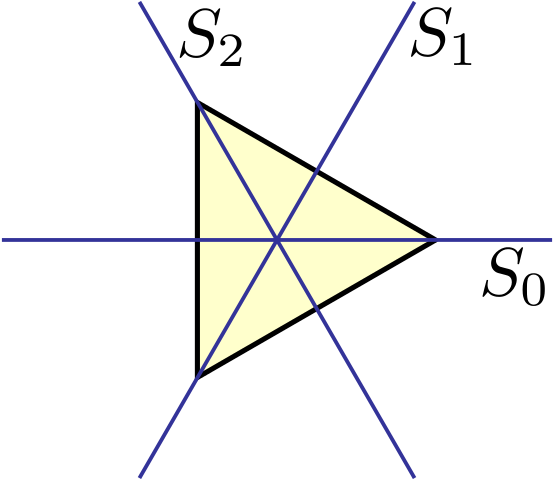
\includegraphics[width=0.2\textwidth]{images/chapter1/TriangleReflections.png}}
\end{wrapfigure}

For example, one may consider the collection of symmetries of an equilateral triangle. What actions could one perform to make the triangle ``look the same'' as before applying the action? Well, we could do nothing. That action is called the \textit{identity action}. We could also reflect the triangle about the line $S_0$ and observe that the triangle ``looks the same as before''. We may also reflect the triangle about the lines $S_1$ and $S_2$, and the triangle will still look the same as before. One may also consider rotating the triangle $120^\circ$ or $240^\circ$ about the centre in a clockwise manner (note that rotating the triangle $360^\circ$ is the same as the identity action, so we do not count it here).

So, in total, we can count 6 distinct actions:
\begin{itemize}
    \item 1 identity action
    \item 2 rotation actions
    \item 3 reflection actions
\end{itemize}
So we can say that the \textit{group of symmetries of the triangle} has 6 actions (or elements) in total.

\begin{wrapfigure}{r}{0.25\textwidth}
    \centering
    \fbox{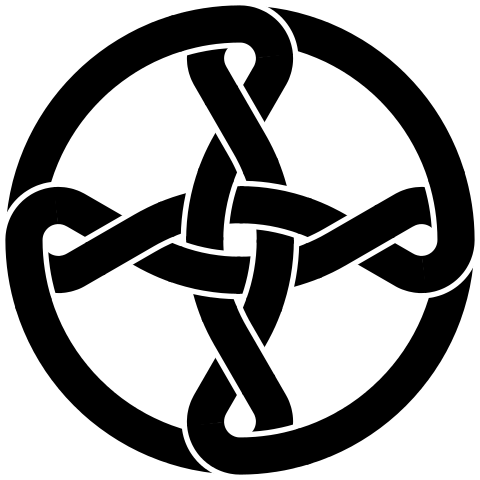
\includegraphics[width=0.2\textwidth]{images/chapter1/CircularCrossings.png}}
\end{wrapfigure}

Another set of groups that we can consider is \textit{groups of rotation}. For example, consider the image on the right. There are 4 actions that we can do to this image that makes it ``look the same as before'':
\begin{itemize}
    \item Do nothing (the identity action).
    \item Rotate the circle $90^\circ$ clockwise.
    \item Rotate the circle $180^\circ$ clockwise.
    \item Rotate the circle $270^\circ$ clockwise.
\end{itemize}
This image has \textbf{no} lines of symmetry. Due to the unique braiding on the knots, this image only has \textit{rotational symmetry} and not \textit{mirror} (or \textit{reflective}) \textit{symmetry}. Thus, this group has only 4 actions that are all rotations. One could say that this group is a \textit{cyclic group} and that it has \textit{order} 4 (we’ll formally define what these terms mean in later chapters).

\begin{wrapfigure}{r}{0.25\textwidth}
    \centering
    \fbox{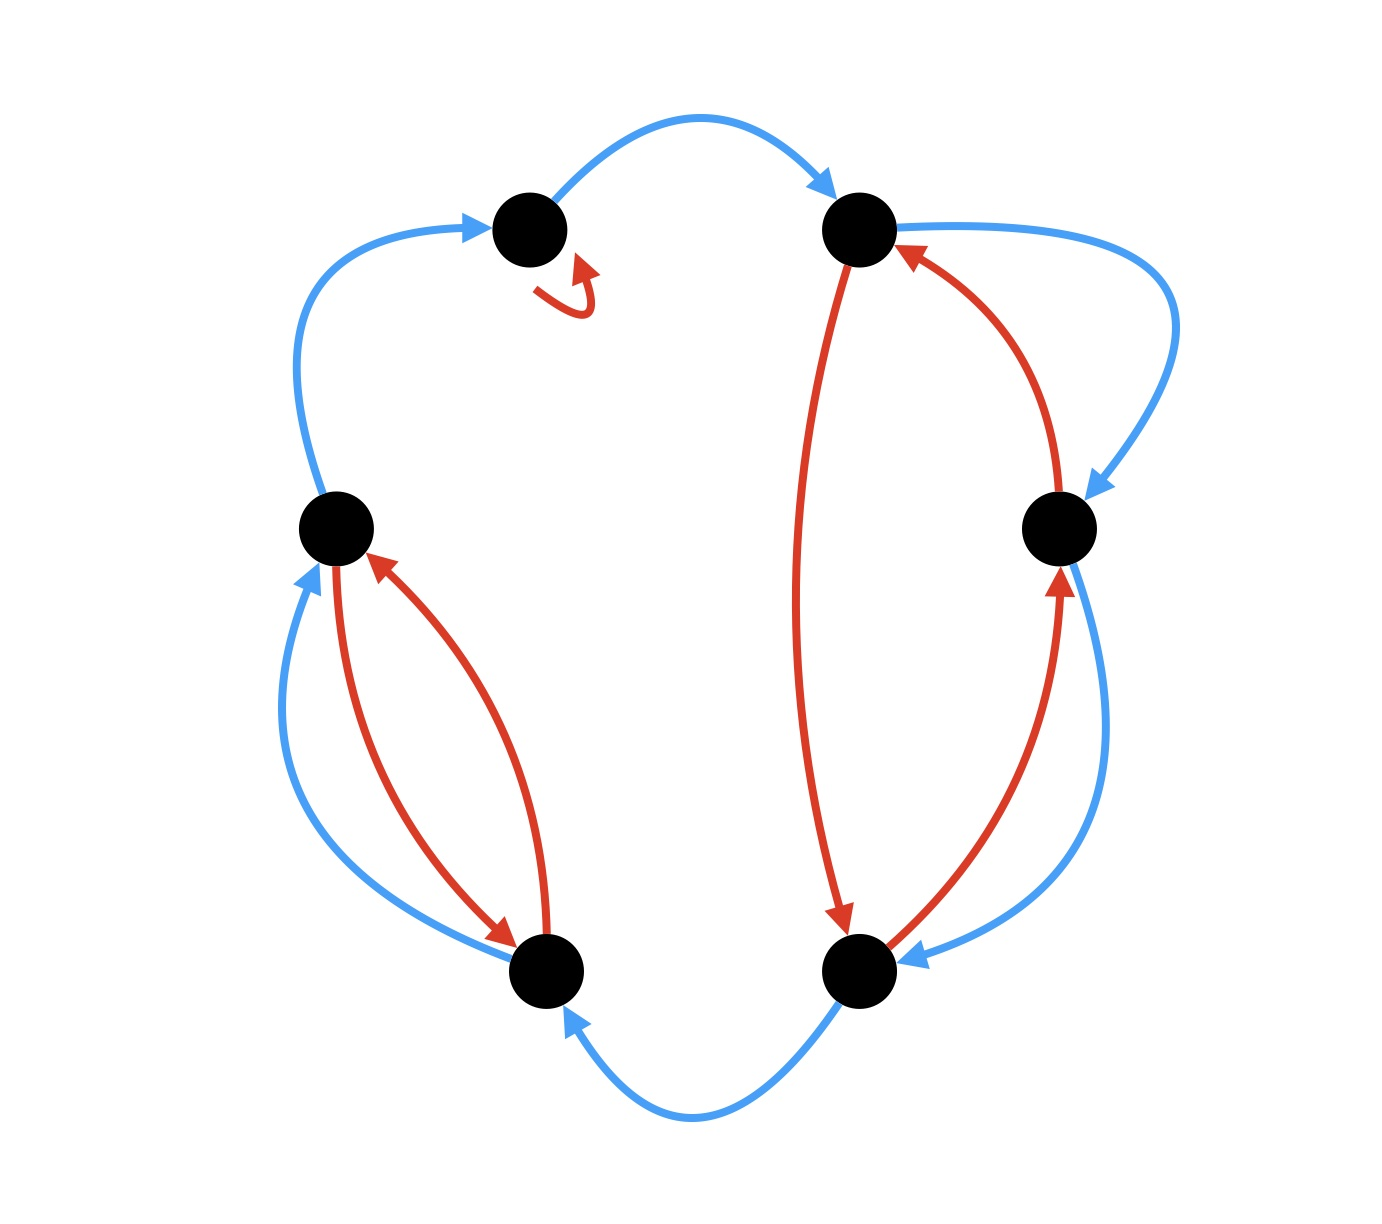
\includegraphics[width=0.2\textwidth]{images/chapter1/Permutations.jpg}}
\end{wrapfigure}

Let’s look at a more technical example: consider a set of points in a pane. We can consider the \textit{group of symmetries of a finite collection of points}. What are the symmetries of the points? Well, in this case, a \textit{symmetry} is a way to move one of these points to another point whilst making it ``look the same as before''.

\begin{itemize}
    \item One possible symmetry is given by the red arrows. In such a symmetry, we have a cycle of 3 points on the right, a cycle of 2 points on the left, and a point mapping to itself. Since the points ``look the same as before'', this is one valid symmetry.
    \item Another possible symmetry is given by the blue arrows. In this case, all points are shifted in a circle. Since the points ``look the same as before'', this is a valid symmetry.
\end{itemize}

One may notice that what each of the symmetries is doing is \textit{permuting} the points around. In this case, this is exactly what each of the symmetries is doing: generating a possible permutation of points and ensuring that their locations stay the same. This is thus called the \textit{symmetric group of degree 6}, and its group actions compose of \textit{bijections from the set to itself}.

\begin{exercise}
    How many symmetries are there in the symmetric group of degree 6? In other words, what is the order of the group above? (\textit{Hint: Consider the number of permutations in the group.})
\end{exercise}

\section{What Constitutes a Group?}
Now that we have taken a look at some examples of groups, we now ask: what properties do all groups satisfy? What properties do all collections of symmetries satisfy?

These properties are known as the \textbf{axioms of groups}. We motivate the `discovery’ of such properties with examples.

\begin{wrapfigure}{r}{0.25\textwidth}
    \centering
    \fbox{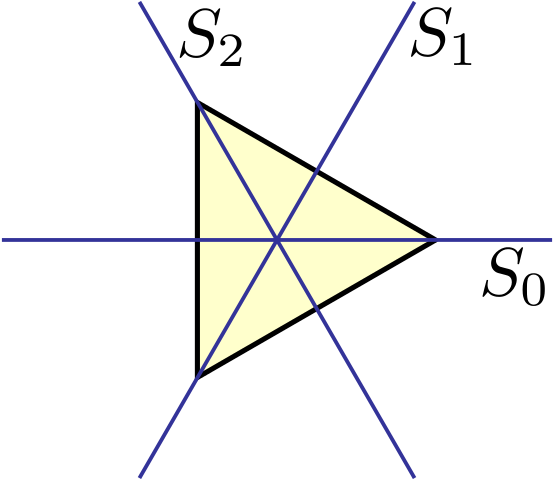
\includegraphics[width=0.2\textwidth]{images/chapter1/TriangleReflections.png}}
\end{wrapfigure}

Consider the group of symmetries of an equilateral triangle. One condition that the group of symmetries must satisfy is that performing group actions one after another should not make the underlying object ``non-symmetric''. We should not be able to apply group actions to other group actions until we obtain an action that results in the triangle being ``non-symmetric''. For example, we do not include rotating the triangle 90° clockwise about the line $S_0$ (into 3D space) as this immediately makes the triangle `different to how it began'.

This property can be called the \textbf{axiom of closure} and can be written like this:
\begin{quote}
    A group $(G, \ast)$ is a set $G$ together with a binary operation $\ast$ that ensures closure. That is, for any element $a$ and $b$ in the set $G$, we must ensure $a \ast b$ is in $G$.
\end{quote}
(Of course, this is not the full definition, but we'll get into the other properties later.)

In the above example, the set $G$ is the set of actions on the equilateral triangle that preserves symmetry. The binary operation $\ast$ is said to be the ``followed by'' operator. Thus:
\begin{quote}
    reflect about $S_0$ $\ast$ rotate the triangle 120° clockwise
\end{quote}
means
\begin{quote}
    rotate the triangle 120° clockwise, \textit{followed by} reflection about $S_0$
\end{quote}
in standard English. In later chapters, such actions will be replaced with symbols. It should also be noted that we read actions \textbf{from right to left}, as seen in the example above.

Another property that a group must have is the identity element. We emphasised this property numerous times in the above examples. This is called the \textbf{axiom of identity} and is phrased as follows:
\begin{quote}
    A group $(G, \ast)$ has an element $e$ where for any element $x$ in $(G, \ast)$, it satisfies $e \ast x = x \ast e = x$.
\end{quote}
This means that the identity action should do nothing. Applying the action before or after another action should just perform the action.

We would also like, for every action, to have an action that \textit{undoes} the previous action. For example, for rotation, we would like to \textit{un-rotate} the rotation. This action is called the \textit{inverse} of the action, and the \textbf{axiom of inverse} guarantees that every action in a group has an inverse:
\begin{quote}
    For every element $x$ in the group $(G, \ast)$, there exists an action in the group, called the inverse of $x$ and denoted by $x^{-1}$, such that $x \ast x^{-1} = x^{-1} \ast x = e$.
\end{quote}

\newpage

\begin{wrapfigure}{r}{0.25\textwidth}
    \centering
    \fbox{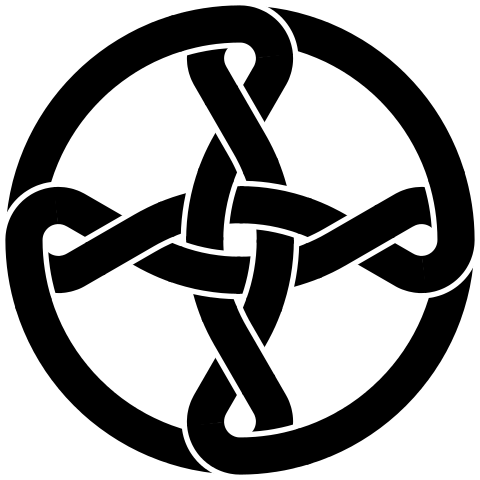
\includegraphics[width=0.2\textwidth]{images/chapter1/CircularCrossings.png}}
\end{wrapfigure}

The last axiom is hard to discover naturally and hard to motivate, but is absolutely necessary for the definition of a group. Consider again this braided circle, and let's say we want to perform 3 rotations (say, $r_1$, $r_2$ and $r_3$) in that sequence. We would not want to differentiate between performing ``$r_1$, then $r_2$ and $r_3$'' (i.e., $r_1 \ast (r_2 \ast r_3)$), and between performing ``$r_1$ then $r_2$, then $r_3$'' (i.e. $(r_1 \ast r_2) \ast r_3$). We are only concerned about the \textit{sequence} of the rotations. This is technically called the \textbf{axiom of associativity}:
\begin{quote}
    Let $x, y$, and $z$ be elements in $(G, \ast)$. Then $(x \ast y) \ast z = x \ast (y \ast z)$.
\end{quote}

So what is a group? A rigorous, careful, and mathematical definition of a group is as follows:
\begin{definition}
    A group is a set $G$ together with a operation on $G$, here denoted by $\ast$, satisfying the following conditions:
    \begin{enumerate}
        \item \textbf{Closure}: For all elements $a$ and $b$ in $G$, $a \ast b$ is also in $G$.
        \item \textbf{Associativity}: For all elements $a, b$, and $c$ in $G$, we have $a \ast (b \ast c) = (a \ast b) \ast c$.
        \item \textbf{Identity}: There exists an element $e$ in $G$ such that for any element $x$ in $G$ we have $e \ast x = x \ast e = x$.
        \item \textbf{Inverse}: For every element $x$ in $G$, there exists an element $x^{-1}$ in $G$ such that $x \ast x^{-1} = x^{-1} \ast x = e$.
    \end{enumerate}
\end{definition}

Usually, for the brevity of notation, we will write $a \ast b$ as $ab$. We will look at more properties of groups in later chapters. We would usually suppress the operation $\ast$ when defining a group, so instead of saying that the group is $(G, \ast)$, we just say that the group is $G$.

\newpage

\section{Problems}
\begin{problem}
Determine whether the following are groups. If they are, prove it. If not, explain why they are not groups.
\begin{enumerate}[label=(\alph*)]
    \item $(\mathbb{Z}, +)$.
    \item $(\mathbb{Z} \setminus \{0\}, \times)$ where $\times$ denotes regular multiplication.
    \item $(\mathbb{R} \setminus \{0\}, \times)$ where $\times$ denotes regular multiplication.
    \item $(\{0\}, \times)$ where $\times$ denotes regular multiplication.
    \item $(\{1\}, +)$ where $+$ denotes regular addition.
    \item $(\{1\}, \times)$ where $\times$ denotes regular multiplication.
\end{enumerate}
\end{problem}

%=========================================
\chapter{Basics of Groups}
\section{Basic Examples of Groups}
Recall that a group has 4 axioms:
\begin{enumerate}
    \item \textbf{Closure}: For all elements $a$ and $b$ in $G$, $a \ast b$ is also in $G$.
    \item \textbf{Associativity}: For all elements $a, b$, and $c$ in $G$, we have $a \ast (b \ast c) = (a \ast b) \ast c$.
    \item \textbf{Identity}: There exists an element $e$ in $G$ such that for any element $x$ in $G$ we have $e \ast x = x \ast e = x$.
    \item \textbf{Inverse}: For every element $x$ in $G$, there exists an element $x^{-1}$ in $G$ such that $x \ast x^{-1} = x^{-1} \ast x = e$.
\end{enumerate}

Recall also we write $a \ast b$ as $ab$, and say that the group $(G, \ast)$ is just $G$ (suppressing the $\ast$).

\begin{remark}
    If the group operation is additive, we write $a + b$ instead of $ab$.
\end{remark}

Let's look at some examples of groups:
\begin{example}
    Let $\mathbb{Z}$ be the set of integers and let $+$ denote regular addition. Then $(\mathbb{Z}, +)$ forms a group:
    \begin{enumerate}
        \item \textbf{Closure}: For all integers $a$ and $b$, we know $a + b$ is an integer.
        \item \textbf{Associativity}: We know $a + (b + c) = (a + b) + c$.
        \item \textbf{Identity}: The identity is 0, since $0 + x = x + 0 = x$.
        \item \textbf{Inverse}: The inverse of integer $x$ is $-x$, since $x + (-x) = (-x) + x = 0$.
    \end{enumerate}
\end{example}

An important thing to note about $(\mathbb{Z}, +)$ is that $+$ is \textit{commutative}: $a + b = b + a$. A group with a commutative operation is called a \textbf{commutative group}. However, it is more often called an \textbf{abelian group}, named after Norwegian mathematician Niels Henrik Abel.

We now look at the notion of $\mathbb{Z}_n$.
\begin{definition}
    The set $\mathbb{Z}_n = \{0, 1, 2, \dots, n-1\}$ where $n$ is a non-negative integer.
\end{definition}
\begin{remark}
    Some sources (e.g. \cite{clark_1984, humphreys_1996}) define $\mathbb{Z}_n$ as a set of congruence classes modulo $n$, i.e. $\mathbb{Z}/n\mathbb{Z}$. We will show that these two definitions are equivalent in a future chapter.
\end{remark}
\begin{proposition}
    The set $\mathbb{Z}_n$ with the operation $\oplus_n$ such that $a \oplus_n b = (a + b) \pmod{n}$ forms a group.
\end{proposition}
\begin{proof}
    We prove this by showing the group axioms hold.
    \begin{enumerate}
        \item \textbf{Closure}: For $a$ and $b$ in $\mathbb{Z}_n$, $a \oplus_n b = (a + b) \pmod{n}$ is a integer between 0 and $n - 1$. Thus $a \oplus b$ is inside $\mathbb{Z}_n$.
        \item \textbf{Associativity}: For $a$, $b$, and $c$ in $\mathbb{Z}_n$, since addition is associative, thus $a \oplus_n (b \oplus_n c) = (a + (b + c)) \pmod{n} = ((a + b) + c) \pmod{n} = (a \oplus_n b) \oplus_n c$.
        \item \textbf{Identity}: The identity is $0$ since for every $x$ in $\mathbb{Z}_n$, $0 \oplus_n x = (0 + x) \pmod{n} = (x + 0) \pmod{n} = x \oplus_n 0 = x$.
        \item \textbf{Inverse}: For inverses, \begin{itemize}
            \item $0$ is its own inverse since $0 \oplus_n 0 = 0$ which is the identity.
            \item For any other integer $x$ in $\mathbb{Z}_n$, the inverse is $n - x$. Since $1 \leq x \leq n - 1$, thus $1 \leq n - x \leq n - 1$ so $n - x$ is indeed in $\mathbb{Z}_n$. Also, $x \oplus_n (n - x) = (x + (n - x)) \pmod{n} = n \pmod{n} = 0$ and $(n - x) \oplus_n x = ((n-x) + x)\pmod{n} = n \pmod{n} = 0$.
        \end{itemize}
    \end{enumerate}
    Since the four group axioms are satisfied, this is a group.
\end{proof}

One could use a \textbf{Cayley table} (or \textbf{group table}) to show that a structure is a group.
\begin{example}
    We show that $(\mathbb{Z}_6, \oplus_6)$ is a group.
    \begin{table}[h]
        \centering
        \begin{tabular}{|l|l|l|l|l|l|l|}
        \hline
        \textbf{$\oplus_6$} & \textbf{0} & \textbf{1} & \textbf{2} & \textbf{3} & \textbf{4} & \textbf{5} \\ \hline
        \textbf{0}          & 0          & 1          & 2          & 3          & 4          & 5          \\ \hline
        \textbf{1}          & 1          & 2          & 3          & 4          & 5          & 0          \\ \hline
        \textbf{2}          & 2          & 3          & 4          & 5          & 0          & 1          \\ \hline
        \textbf{3}          & 3          & 4          & 5          & 0          & 1          & 2          \\ \hline
        \textbf{4}          & 4          & 5          & 0          & 1          & 2          & 3          \\ \hline
        \textbf{5}          & 5          & 0          & 1          & 2          & 3          & 4          \\ \hline
        \end{tabular}
    \end{table}
    Note that:
    \begin{enumerate}
        \item For all $x$ and $y$ in $\mathbb{Z}_6$, $x \oplus_6 y$ is in $\mathbb{Z}_6$ from the above table.
        \item For all $x, y$, and $z$ in $\mathbb{Z}_6$, $x \oplus_6 (y \oplus_6 z) = (x \oplus_6 y) \oplus_6 z$ from the above table.
        \item 0 is the identity since adding anything to it returns the original number.
        \item Every row has an integer that when added gives 0.
    \end{enumerate}
    Thus $(\mathbb{Z}_6, \oplus_6)$ is a group.
\end{example}

It should be noted that we use the convention of reading the \textbf{row before the column} in a group table. However, since this is an abelian group, the order does not matter. We will look at Cayley tables of non-abelian groups later.

\begin{exercise}
    Let $a \otimes_n b = (a \times b) \pmod{n}$. By using a group table, show that $(\mathbb{Z}_6, \otimes_6)$ does \textbf{not} form a group.
\end{exercise}

\newpage

\section{General Properties of Groups}
Before we get into the general properties of groups, we introduce a useful notation for repeated application of $\ast$ on a single element $a$ in the group $G$.
\begin{definition}
    Let $a$ be an element in $G$. Then
    \[
        a^n =
        \begin{cases}
        a\ast a\ast \cdots \ast a & \text{ if } n > 0 \ (n\text{ copies of }a)\\
        e & \text{ if } n=0 \\
        a^{-1}\ast a^{-1}\ast\cdots \ast a^{-1} & \text{ if } n<0 \ (|n|\text{ copies of }a^{-1})
        \end{cases}
    \]
\end{definition}

Note that some laws of exponents apply to the above operation:
\begin{itemize}
    \item $\left(a^{-1}\right)^m = \left(a^m\right)^{-1}$
    \item $a^{m+n} = a^m \ast a^n$
    \item $\left(a^m\right)^n = a^{mn}$
\end{itemize}
Proof of these properties are left as an exercise for the reader.

We are now ready to prove some properties of groups.
\begin{proposition}
    The identity of a group $G$ is unique.
\end{proposition}
\begin{proof}
    Suppose $e_1$ and $e_2$ are identities of the group $G$. Then, for all $x$ in $G$, we have
    \[
        e_1x = xe_1 = x \text{ and } e_2x = xe_2 = x,
    \]
    since they are identities. Thus,
    \begin{align*}
        e_1 &= e_1e_2 & (\text{since } e_2 \text{ is an identity, so } xe_2 = x)\\
        &= e_2 & (\text{since } e_1 \text{ is an identity, so } xe_1 = x)
    \end{align*}
    Therefore $e_1 = e_2$, meaning that the identity is unique.
\end{proof}

\newpage

\begin{proposition}
    $e^{-1} = e$
\end{proposition}
\begin{proof}
    Clearly $e = ee^{-1}$ since $xx^{-1} = e$ for all elements $x$ in $G$, including $x = e$. Also, $ee^{-1} = e^{-1}$ since $e$ is the identity. Thus $e = e^{-1}$.
\end{proof}

\begin{proposition}
    The inverse of an element $x$ of a group $G$ is unique.
\end{proposition}
\begin{proof}
    Suppose that $a$ and $b$ are inverses of $x$. Then we have
    \[
        ax = xa = e \text{ and } bx = xb = e,
    \]
    since $a$ and $b$ are inverses of $x$. Note that
    \begin{align*}
        a &= ae & (\text{since } e \text{ is the identity})\\
        &= a(xb) & (\text{since } b \text{ is an inverse, so } xb = e)\\
        &= (ax)b & (\text{by associativity})\\
        &= eb & (\text{since } a \text{ is an inverse, so } ax = e)\\
        &= b & (\text{since } e \text{ is the identity})
    \end{align*}
    Therefore $a = b$. Thus the inverse of $x$ is unique.
\end{proof}

\begin{proposition}[Shoes and Socks]
    For all elements $x$ and $y$ in $G$, $(ab)^{-1} = b^{-1}a^{-1}$.
\end{proposition}
\begin{proof}
    Recall that if $g^{-1}$ is the inverse of $g$ then $gg^{-1} = g^{-1}g = e$. We will show that $(ab)(b^{-1}a^{-1}) = e$ and $(b^{-1}a^{-1})(ab) = e$.
    \begin{align*}
        (ab)(b^{-1}a^{-1}) &= a(bb^{-1})a^{-1} & (\text{by associativity})\\
        &= a(e)a^{-1} & (\text{since } bb^{-1} = e)\\
        &= aa^{-1} & (\text{since } e \text{ is the identity})\\
        &= e & (\text{since } aa^{-1} = e),
    \end{align*}
    and,
    \begin{align*}
        (b^{-1}a^{-1})(ab) &= b^{-1}(a^{-1}a)b & (\text{by associativity})\\
        &= b^{-1}(e)b & (\text{since } a^{-1}a = e)\\
        &= b^{-1}b & (\text{since } e \text{ is the identity})\\
        &= e & (\text{since } b^{-1}b = e).
    \end{align*}
    Thus, $b^{-1}a^{-1}$ is the inverse of $ab$, so $(ab)^{-1} = b^{-1}a^{-1}$
\end{proof}

\begin{exercise}
Prove that for all $x$ in $G$, $\left(x^{-1}\right)^{-1} = x$.
\end{exercise}

We now prove an important property of groups: the \textbf{cancellation law}.
\begin{proposition}[Cancellation Law]
    Let $g$, $x$, and $y$ be elements in the group $G$. Then
    \begin{enumerate}
        \item if $gx=gy$ then $x = y$; and
        \item if $xg=yg$ then $x = y$.
    \end{enumerate}
\end{proposition}
\begin{proof}
    We prove the two cases separately.
    \begin{enumerate}
        \item Suppose $gx = gy$. Then
        \begin{align*}
            &g^{-1}(gx) = g^{-1}(gy) & (\text{left multiply by } g^{-1})\\
            &(g^{-1}g)x = (g^{-1}g)y & (\text{by associativity})\\
            &ex = ey & (\text{since } g^{-1}g = e)\\
            &x = y & (\text{since } e \text{ is the identity})
        \end{align*}
        \item Suppose $xg = yg$. Then
        \begin{align*}
            &(xg)g^{-1} = (yg)g^{-1} & (\text{right multiply by } g^{-1})\\
            &x(gg^{-1}) = y(gg^{-1}) & (\text{by associativity})\\
            &xe = ye & (\text{since } gg^{-1} = e)\\
            &x = y & (\text{since } e \text{ is the identity})
        \end{align*}
    \end{enumerate}
    This completes the proof.
\end{proof}

\section{Order of a Group and Order of an Element}
We look at the notion of \textit{order} with respect to groups and elements of a group.

\begin{definition}
    Let $G$ be a group. The order of a group, denoted by $|G|$, is the number of elements in the set $G$.
\end{definition}

If $|G| = n$ where $n$ is finite, we say that $G$ is a \textbf{finite group}. On the other hand, if $|G| = \infty$, then we say that $G$ is an \textbf{infinite group}.

\begin{example}
    The group $(\mathbb{Z}_4, \oplus_4)$ has order 4 since it has 4 elements: 0, 1, 2, and 3.
\end{example}

\begin{example}
    The group $(\mathbb{R}, +)$ is an infinite group since $\mathbb{R}$ has an uncountably infinite number of elements.
\end{example}

Let's now look at the order of an element:
\begin{definition}
    Let $g$ be an element of the group $G$. Then the order of $g$, denoted by $|g|$, is the least positive integer $n$ such that $g^n = e$.
\end{definition}
Note that if $n$ is infinite, we say that the order of $g$ is infinite.

\begin{example}
    Consider the group $(\mathbb{Z}_4, \oplus_4)$ and its 4 elements 0, 1, 2, and 3.
    \begin{itemize}
        \item The element $0$ has order 1 since $0 = 0$ which is the identity. Thus $|0| = 1$ in $(\mathbb{Z}_4, \oplus_4)$.
        \item The element $1$ has order 4 since $1 \oplus_4 1 \oplus_4 1 \oplus_4 1 = 0$ and no smaller $n$ than 4 exists. Thus $|1| = 4$ in $(\mathbb{Z}_4, \oplus_4)$.
        \item The element $2$ has order 2 since $2 \oplus_4 2 = 0$ and no smaller $n$ than 2 exists. Thus $|2| = 2$ in $(\mathbb{Z}_4, \oplus_4)$.
        \item The element $3$ has order 4 since $3 \oplus_4 3 \oplus_4 3 \oplus_4 3 = 0$ and no smaller $n$ than 4 exists. Thus $|3| = 4$ in $(\mathbb{Z}_4, \oplus_4)$.
    \end{itemize}
\end{example}

\newpage

We note a few things about the order of elements in a group.
\begin{itemize}
    \item The identity element always has order 1.
    \item A group in which every element has finite order is said to be \textbf{periodic}.
    \item A finite group is always periodic because all elements in a finite group has finite order.
    \item The order of any element in a group divides the order of the group.
\end{itemize}
The last point is actually a corollary of Lagrange's Theorem (\textbf{Theorem \ref{thrm-lagrange}}). We will look into the proof it in the next chapter.

\begin{exercise}
    Let $i$ be a number such that $i^2 = -1$. Let $\mathcal{S} = \{1, -1, i, -i\}$.
    \begin{enumerate}[label=(\roman*)]
        \item Find the identity of the group $(\mathcal{S}, \times)$ where $\times$ denotes regular multiplication.
        \item Find the orders of the elements of the above group.
    \end{enumerate}
\end{exercise}

\section{Cyclic Groups}
Now that we have gotten some basic terminology and properties of groups out of the way, let's introduce a very simple type of group: the cyclic groups.

Suppose we have an element $g$ belonging to a group $G$. Suppose that the entire set $G$ is \textit{generated} by $g$, that is, the set
\[
    G = \{g, g^2, g^3, g^4, \dots, g^n\}
\]
for some positive integer $n$. Then, we say that $G$ is a \textbf{cyclic group of order $n$} and has a \textbf{generator} of $g$. Notationally, we write $G = \langle g \rangle$.

\begin{example}
    Let $i$ be the imaginary unit, i.e. $i^2 = -1$. Let $\mathcal{S} = \{1, -1, i, -i\}$. Notice the group $(\mathcal{S}, \times)$ is completely generated by the element $i$ since
    \[
    i^1 = i, i^2 = -1, i^3 = -i, \text{ and } i^4 = 1.
    \]
    Thus, $\mathcal{S} = \{i, i^2, i^3, i^4\} = \langle i \rangle$.
\end{example}

\begin{exercise}
    Using the set $\mathcal{S}$ from the above example, find the other generator of the group $(\mathcal{S}, \times)$.
\end{exercise}

It should be noted that not every element in a cyclic group is a generator, and that a cyclic group may have more than 1 generator.

Cyclic groups may also be of \textbf{infinite order}. Such cyclic groups are called \textbf{cyclic groups of infinite order} or \textbf{infinite cyclic groups}.
\begin{example}
    The group $(\mathbb{Z}, +)$ is an infinite cyclic group with generators 1 and -1.
\end{example}

We now look at two results involving cyclic groups.

\begin{proposition}\label{prop-cyclic-group-is-abelian}
    Every cyclic group is abelian.
\end{proposition}
\begin{proof}
    Let $G$ be the cyclic group with a generator $g$. Suppose $x$ and $y$ are elements in $g$. Thus, $x = g^m$ and $y = g^n$ for some integers $m$ and $n$.

    Thus, we have the following:
    \begin{align*}
        xy &= (g^m)(g^n)\\
        &= g^mg^n\\
        &= g^{m+n}\\
        &= g^{n+m} & (\text{since + is commutative})\\
        &= g^ng^m\\
        &= (g^n)(g^m)\\
        &= yx
    \end{align*}
    so $xy = yx$. Therefore $G$ is abelian.
\end{proof}

\begin{theorem}\label{thrm-cyclic-group-has-element-with-same-order}
    A finite group $G$ is cyclic if and only if there exists an element $g$ in the group $G$ with the same order as the group.
\end{theorem}
\begin{proof}
    We first prove the forward direction: suppose $G$ is cyclic and $|G| = n$. Then there exists an element $g$ in $G$ such that
    \[
        G = \langle g \rangle = \{g^k \ | \ 1 \leq k \leq n, k \in \mathbb{Z}\},
    \]
    by definition (i.e. $g$ is a generator of $G$). We just need to show $|g| = n$.

    Suppose on the contrary there exists an integer $1 \leq m < n$ where $g^m = e$. Then $\langle g \rangle = \{g, g^2, \dots, g^m\}$. Thus $|\langle g \rangle| = m < n = |G|$. But by the hypothesis of the forward direction, $G = \langle g \rangle$ so $n = |G| = |\langle g \rangle| = m$. This is a contradiction, i.e. there does \textbf{not} exist an integer $1 \leq m < n$ where $g^m = e$. Therefore $g^n = e$, i.e. $|g| = n$.

    We now prove the reverse direction: suppose there exists an element $g$ in $G$ with order $n$. We claim that $g, g^2, \dots, g^n$ are all distinct.

    Suppose on the contrary that there exist integers $i$ and $j$ where $1 \leq i < j \leq n$ such that $g^i = g^j$. Then:
    \[
        g^i = g^ig^{j-i} \implies g^{j-i} = e
    \]
    by the cancellation law. Note that $1 \leq j - i < n$. Thus, since $g^{j-i} = e$, therefore $|g| = j - i < n$ which contradicts $|g| = n$.

    Hence, $g, g^2, \dots, g^n$ are all distinct. Therefore, $\langle g \rangle = \{g, g^2, \dots, g^n\}$ contain distinct elements of $G$. But there are only $n$ elements in $G$ and $\langle g \rangle$ contains $n$ distinct elements. Therefore, $G = \langle g \rangle$ which means that $G$ is cyclic with generator $g$.

    This completes the proof.
\end{proof}

There are more interesting properties of cyclic groups, but we will get to them when we develop more tools to explain and prove these properties.

\section{Dihedral Groups}
We motivate the definition of the dihedral groups by discussing the symmetries of an equilateral triangle.

\begin{figure}[h]
    \centering
    \fbox{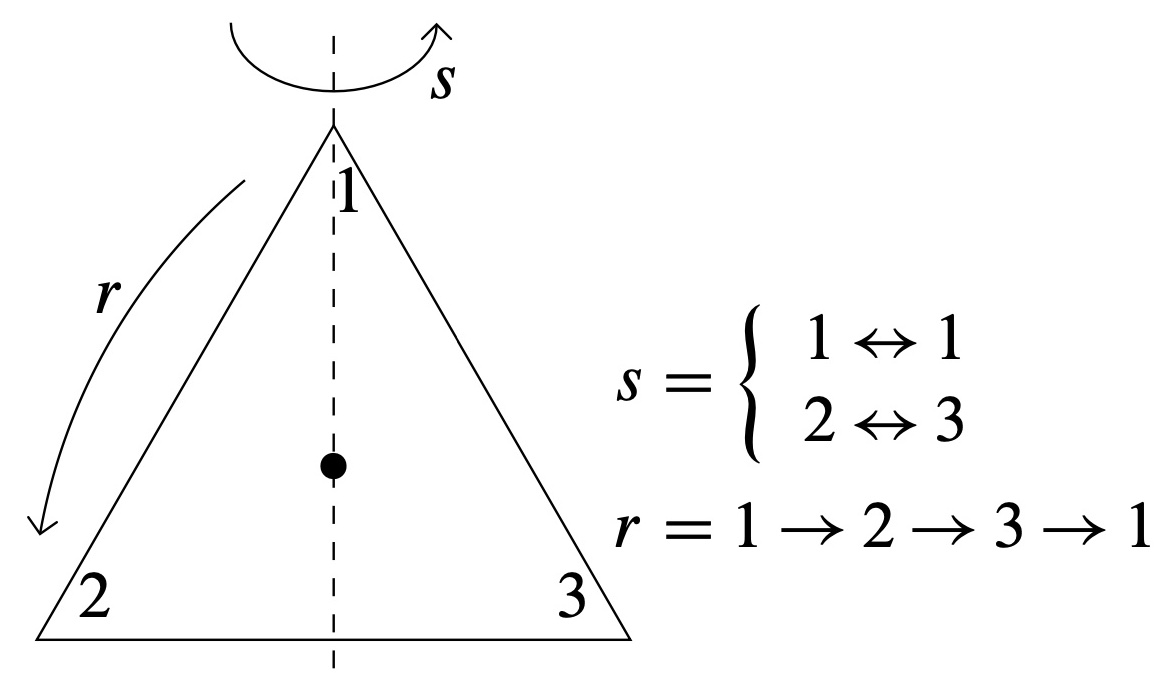
\includegraphics[width=6cm]{images/chapter2/GroupD3.jpg}}
    \caption{Symmetries of an Equilateral Triangle}
\end{figure}

Look at that equilateral triangle. What actions could we perform in order to maintain symmetry? Well, we could rotate the triangle in $120^\circ$ anti-clockwise increments about the center of the triangle. We denote this action by the symbol $r$. Another thing we could do is reflect the triangle about the line going through one of the vertices and the center, like we discussed in Chapter 1. This action is denoted by $s$.

Now, suppose we define $r$ to be the $120^\circ$ anti-clockwise rotation about the center and $s$ be the reflection of the triangle about the line going through vertex 1 and the center, like shown in the diagram. How do we obtain a $240^\circ$ anti-clockwise rotation? Well, we apply two $120^\circ$ anticlockwise rotations one after another. In other words, if $\ast$ means ``action composition'', then a $240^\circ$ rotation would be represented by $r^2$. Note that $r^3$, which represents a $360^\circ$ anti-clockwise rotation, is the same as doing nothing. Thus, $r^3 = e$. Similarly, applying the reflection $s$ twice in a row (i.e., $s^2$) is the same as doing nothing. Thus, we have
\[
    r^3 = s^2 = e
\]
for the case of an equilateral triangle.

There's another relationship governing $r$ and $s$. Consider this: how do we obtain a reflection about the line through vertex 3 and the center? Well, we apply $r$ first, followed by $s$. This means that a reflection about the line through vertex 3 and the center is given by $rs$. Notice that this is the same thing as reflecting first and then applying $r$ twice, i.e. $sr^2$. Thus, we have the second relationship:
\[
    rs = sr^2
\]
for the case of an equilateral triangle.

The group of symmetries of an equilateral triangle is called the \textbf{dihedral group of order 6} and is denoted by $D_3$. In general, the \textbf{dihedral group of order $2n$} is denoted by $D_n$ and can be thought of as the symmetries of a regular polygon of $n$ sides (a regular $n$-gon). For example, the symmetries of the square is given by the group $D_4$.

\begin{figure}[h]
    \centering
    \fbox{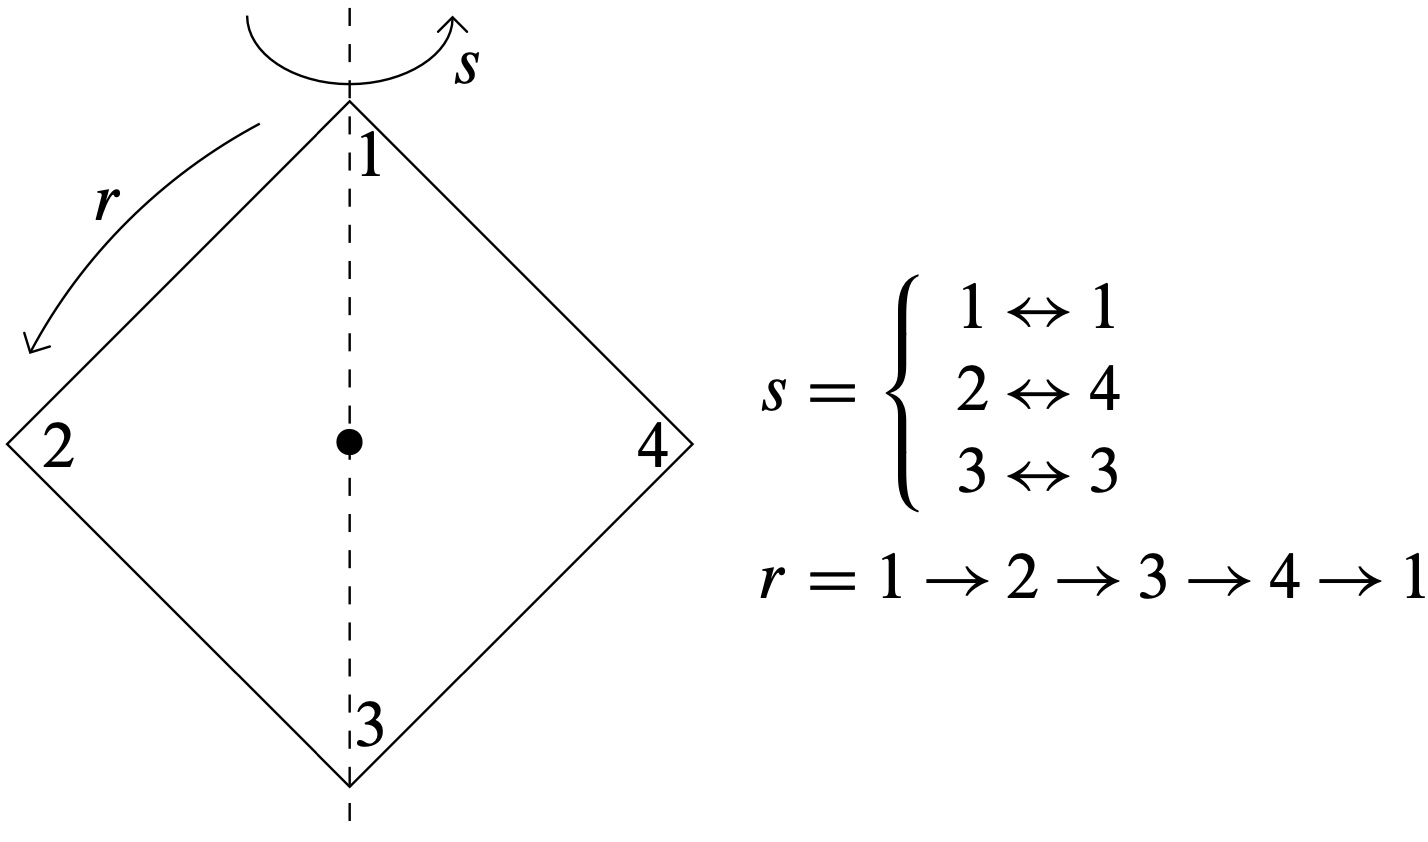
\includegraphics[width=6cm]{images/chapter2/GroupD4.jpg}}
    \caption{Symmetries of a Square}
\end{figure}

Thus, in general, the \textit{set} $D_n$ consists of the following elements.
\[
    D_n = \{e, r, r^2, \dots, r^{n-1}, s, rs, r^2s, \dots, r^{n-1}s\}
\]
with the relationship between $r$ and $s$ given by $r^n = s^2 = e$ and $rs = sr^{n-1}$.

\begin{remark}
    Some authors (e.g. \cite{humphreys_1996}) will write the reflections of $D_n$ with $s$ leading the $r$, i.e. $s, sr, sr^2, sr^3, \dots, sr^{n-1}$. However the underlying definition remains the same.
\end{remark}

These relationships are succinctly given by the \textit{presentation}
\[
    D_n = \langle r, s \ | \ r^n = s^2 = e, rs = sr^{n-1} \rangle
\]
where $r$ and $s$ can be thought of as `generators' and the conditions are given on the right side of the pipe ($|$).

\begin{example}\label{example-presentation-of-D3}
    We look at the group $D_3$ which has presentation
    \[
        D_3 = \langle r, s \ | \ r^3 = s^2 = e, rs = sr^2 \rangle.
    \]
    The Cayley table of the group is given below.

    \begin{table}[h]
        \centering
        \begin{tabular}{|l|l|l|l|l|l|l|}
        \hline
        $\ast$ & $e$    & $r$    & $r^2$  & $s$    & $rs$   & $r^2s$ \\ \hline
        $e$    & $e$    & $r$    & $r^2$  & $s$    & $rs$   & $r^2s$ \\ \hline
        $r$    & $r$    & $r^2$  & $e$    & $rs$   & $r^2s$ & $s$    \\ \hline
        $r^2$  & $r^2$  & $e$    & $r$    & $r^2s$ & $s$    & $rs$   \\ \hline
        $s$    & $s$    & $r^2s$ & $rs$   & $e$    & $r^2$  & $r$    \\ \hline
        $rs$   & $rs$   & $s$    & $r^2s$ & $r$    & $e$    & $r^2$  \\ \hline
        $r^2s$ & $r^2s$ & $rs$   & $s$    & $r^2$  & $r$    & $e$    \\ \hline
        \end{tabular}
    \end{table}

    It should be noted that we use the convention of reading the \textbf{row before the column}. So the action $rs \ast r^2$ (which is usually written as $rsr^2$) is given by the row of $rs$ and the column of $r^2$, which is $r^2s$.
\end{example}

The \textit{cannonical form} of an element in a dihedral group is of the form $r^ms^n$ where $m$ and $n$ are non-negative integers. So how do we find the canonical form of elements like $sr$ or $srs$? We have this useful proposition to help:
\begin{proposition}
    For the group $D_n$, we have $r^ms = sr^{n-m}$ for all integers $1 \leq m < n$.
\end{proposition}
\begin{proof}
    We prove this claim using induction on $m$.

    When $m = 1$, $rs = sr^{n-1}$ is given by the definition of the group $D_n$.

    Assume now that for some integer $1 \leq k < n$, we have $r^ks = sr^{n-k}$. We consider two cases.
    \begin{itemize}
        \item If $k = n - 1$, then $k + 1 = n$. Thus, $r^{k+1}s = r^ns = s$ since $r^n = e$. Note that $sr^{(k+1)-n} = sr^{n-n} = sr^0 = s$. Therefore $r^{k+1}s = sr^{(k+1)-n}$ for the case when $k = n - 1$.
        \item The other case is if $1 \leq k \leq n - 2$. Then we have:
        \begin{align*}
            r^{k+1}s &= r^k(rs)\\
            &= r^k(sr^{n-1}) & (\text{base case})\\
            &= (r^ks)r^{n-1} & (\text{associativity})\\
            &= (sr^{n-k})r^{n-1} & (\text{by Induction Hypothesis})\\
            &= sr^{2n - k - 1}\\
            &= sr^nr^{n-k-1}\\
            &= sr^{n-(k+1)} & (\text{since } r^n = e)
        \end{align*}
    \end{itemize}
    Therefore this applies to the subsequent case of $k+1$.

    Hence $r^ms = sr^{n-m}$ for all integers $1 \leq m < n$.
\end{proof}

\begin{exercise}
    Simplify $rsr^4sr^3$ in the group $D_6$.
\end{exercise}

\newpage

\section{Problems}
\begin{problem}
    Draw the Cayley table for $D_4$, the dihedral group of order 8, representing the symmetries of a square. By referring to the Cayley table,
    \begin{enumerate}[label=(\alph*)]
        \item explain why $D_4$ is \textbf{not} abelian;
        \item simplify $r^3srsr^3sr^3sr^2$.
    \end{enumerate}
\end{problem}

\begin{problem}
    Let $G$ be a group. If every element in $G$ is its own inverse, show that $G$ is abelian.
\end{problem}

\begin{problem}\label{problem-element-to-power-of-multiple-of-order-is-identity}
    Let $G$ be a group with identity $e$. Suppose an element $x$ in $G$ has finite order $k$. Prove that $n$ is a multiple of $k$ if and only if $a^n = e$.\newline
    (\textit{Hint: consider Euclid's division lemma (\textbf{Lemma \ref{lemma-euclid-division}}) to prove one direction of the claim.})
\end{problem}

\begin{problem}
    Let $G$ be a group.
    \begin{enumerate}[label=(\alph*)]
        \item Suppose $(gh)^2 = g^2h^2$ for all elements $g$ and $h$ in $G$. Prove that $G$ is abelian.
        \item Suppose $G$ is abelian. Prove that $(gh)^n = g^nh^n$ for all elements $g$ and $h$ in $G$ and for all positive integers $n$.
    \end{enumerate}
\end{problem}

\begin{problem}
    Prove that $(\mathbb{Z}_n, \oplus_n)$ is a cyclic group of order $n$. (It is given that $(\mathbb{Z}_n, \oplus_n)$ is a group.)
\end{problem}

\begin{problem}
    The set $S = \mathbb{R}^2$, that is,
    \[
        S = \{(x, y) \ | \ x, y \text{ are real numbers}\}.
    \]
    The transformation $T: S \to S$ is defined by
    \[
        T(x, y) = (-y, x+y).
    \]
    Let the set $A = \{T^r \ | \ r \in \mathbb{Z} \text{ and } r \geq 1\}$. Show that $A$ is a group under function composition $\circ$, and give the order of this group.
\end{problem}

%=========================================
\chapter{Subgroups}
\section{Definition and Examples}
We look at the notion of a subgroup of a group.
\begin{definition}
    Let $G$ be a group with operation $\ast$. Let $H \subseteq G$. Then $H$ is said to be a \textbf{subgroup} of $G$ if:
    \begin{enumerate}
        \item \textbf{Closure}: For all $x$ and $y$ in $H$, $x \ast y$ is also in $H$.
        \item \textbf{Identity}: The identity of the group $G$ is in $H$.
        \item \textbf{Inverse}: For all elements $x$ in $H$, there exists an element $x^{-1}$ in $H$ such that $x \ast x^{-1} = x^{-1} \ast x = e$.
    \end{enumerate}
\end{definition}
\begin{remark}
    Equivalently, $H$ is a subgroup of $G$ if $H \subseteq G$ and $H$ is a group under the group operation of $G$.
\end{remark}
We write $H \leq G$ if $H$ is a subgroup of $G$.

\begin{example}
    Let's look at all possible subgroups of the group $(\mathbb{Z}, +)$. Suppose $H \leq G = (\mathbb{Z}, +)$. Suppose also that $H$ is not the trivial subgroup containing only the identity in $(\mathbb{Z}, +)$, i.e. $H \neq \{0\}$.

    Let $n$ be the smallest \textit{positive} integer in $H$. Let $m$ be any \textit{other} number in $H$. Then by the division algorithm, $m = nq + r$ where $q$ and $r$ are integers such that $0 \leq r < n$. Hence,
    \[
        r = m + \underbrace{(-n) +(-n) +(-n) + \cdots + (-n)}_{q\text{ times}}
    \]
    Note that $m$ is in $H$, and $-n$ is also in $H$. Thus, $r = m + (-n) + \cdots + (-n)$ is also in $H$ since $H$ is closed under addition. But, $0 \leq r < n$ and $n$ is the \textit{smallest} positive integer in $H$. Thus, $r \not> 0$ which means $r = 0$. Hence, $m = nq$, i.e. every element in $H$ is a multiple of the smallest positive integer in $H$.

    Hence,
    \[
    H = \{nk \ | \ k \in \mathbb{Z}\},
    \]
    which is often written as the group $n\mathbb{Z}$.
\end{example}

\begin{exercise}
    Let $G$ be a group with operation $\ast$ and identity $e$. Prove that $\{e\} \leq G$.
\end{exercise}

We note that the group containing only the identity (i.e., $\{e\} \leq G$) is always present in every group. This is known as the \textbf{trivial subgroup}. We also note that the group itself is a subgroup of itself (that is, $G \leq G$). Any subgroup that are \textbf{not} these two groups is known as a \textbf{proper subgroup} of $G$, and we write $H < G$ if $H$ is a proper subgroup of $G$.

\section{Subgroup Test}
To prove that a subset of a group is a subgroup using the axioms is too tedious. Wouldn't it be nice if we have a simple test to determine if a subset is a subgroup? Well, there is; it is called the \textbf{subgroup test}.
\begin{proposition}[Subgroup Test]
    Let $G$ be a group and $H \subseteq G$ such that $H \neq \emptyset$ (i.e., $H$ is not the empty set). Then $H \leq G$ if and only if for all $x$ and $y$ in $H$, then $xy^{-1}$ is in $H$.
\end{proposition}
\begin{proof}
    We prove the forward direction first. Suppose $H \leq G$ and let $x$ and $y$ be elements in $H$. Since $H$ is a subgroup of $G$, inverses exist. Thus $y^{-1}$ is in $H$. Also, since $H$ is a subgroup of $G$, thus $H$ is closed under the group operation. Hence, $xy^{-1}$ is in $H$. Therefore, if $H \leq G$ then for all $x$ and $y$ in $H$, $xy^{-1}$ is in $H$.

    We now prove the reverse direction. Suppose for all $x$ and $y$ in $H$, $xy^{-1}$ is in $H$.
    \begin{itemize}
        \item Suppose $h$ is an arbitrary element in $H$. Set $x = h$ and $y = h$. Then $xy^{-1} = hh^{-1} = e$ is in $H$. Thus the identity of $G$ is present in $H$.
        \item Set $x = e$ and let $y = h$. Then $xy^{-1} = eh^{-1} = h^{-1}$ is in $H$. Hence every element in $H$ has an inverse in $H$.
        \item Let $a$ and $b$ be elements in $H$. Then by above point, $b^{-1}$ is in $H$. Set $x = a$ and $y = b^{-1}$. Then $xy^{-1} = a\left(b^{-1}\right)^{-1} = ab$ is in $H$. Hence $H$ is closed under the group operation.
    \end{itemize}
    Therefore, if for all $x$ and $y$ in $H$, $xy^{-1}$ is in $H$, then $H \leq G$.

    This completes the proof of the subgroup test.
\end{proof}

\begin{remark}
We usually show the `non-empty' and `subset' requirement by checking if the identity of $G$ is in $H$.
\end{remark}

We look at some examples of the use of the subgroup test.
\begin{example}\label{example-centralizer-of-a-subset}
    Let $G$ be a group and $S \subseteq G$ where $S \neq \emptyset$. The \textbf{centralizer} of $S$ in $G$ is the set
    \[
        \C{G}{S} = \left\{g \in G \ | \ \text{for all } s \in S \text{ we have } gs = sg\right\}.
    \]
    We claim that $\C{G}{S}$ is a subgroup of $G$.
    \begin{proof}
        We show that for all elements $x$ and $y$ in $\C{G}{S}$, $xy^{-1}$ is also in the centralizer. Note that the condition $gs = sg$ is equivalent to the condition $sg^{-1} = g^{-1}s$.

        Suppose $x$ and $y$ are in $\C{G}{S}$. Let $s$ be in $S$. Then
        \begin{align*}
            (xy^{-1})s &= x(y^{-1}s) & (\text{associativity})\\
            &= x(sy^{-1}) & (\text{since } sg^{-1} = g^{-1}s)\\
            &= (xs)y^{-1} & (\text{associativity})\\
            &= (sx)y^{-1} & (\text{since } gs = sg)\\
            &= s(xy^{-1}) & (\text{associativity})
        \end{align*}
        so $(xy^{-1})s = s(xy^{-1})$ for all $s$ in $S$. Thus, $xy^{-1}$ is in $\C{G}{S}$, so by subgroup test $\C{G}{S} \leq G$.
    \end{proof}
\end{example}
\begin{remark}
    In the case where $S$ has a single element, say $S = \{x\}$, we write $\C{G}{x}$.
\end{remark}

\begin{example}\label{example-center-of-group}
    Let $G$ be a group. The \textbf{center} of a group $G$ is given by the set
    \[
        \Z{G} = \{z \in G \ | \ gz = zg \text{ for all } g \in G\}.
    \]
    We claim that $\Z{G}$ is a subgroup of $G$ under the group operation of $G$.

    \begin{proof}
	    Note that $e \in \Z{G}$ since $ge = eg$ for all $g \in G$.

	    Let $x$ and $y$ be in $\Z{G}$, meaning that $gx = xg$ and $gy = yg$ for all $g \in G$. Note that $gy = yg$ implies $g = ygy^{-1}$ (by right multiplying by $y^{-1}$) which further means that $y^{-1}g = gy^{-1}$ (by left multiplying by $y^{-1}$). Therefore, $y^{-1} \in \Z{G}$. Now,
	    \begin{align*}
	        (xy^{-1})g &= x(y^{-1}g)\\
	        &= x(gy^{-1}) & (\text{since } y^{-1} \in \Z{G})\\
	        &= (xg)y^{-1} & (\text{associativity})\\
	        &= (gx)y^{-1} & (\text{since } x \in \Z{G})\\
	        &= g(xy^{-1}) & (\text{associativity})
	    \end{align*}
	    which means that $xy^{-1} \in \Z{G}$. Hence $\Z{G} \leq G$ by the subgroup test.
    \end{proof}
\end{example}

\begin{exercise}\label{exercise-conjugate-subgroup}
    Let $G$ be a group, $H \leq G$, and $g \in G$. Define the set
    \[
        S = \{ghg^{-1} \ | \ h \text{ is in } H\}.
    \]
    Prove that $S \leq G$ under the group operation of $G$.
\end{exercise}

\newpage

\section{Cosets}
We now introduce the idea of \textbf{cosets} of a group $G$.
\begin{definition}
    Let $G$ be a group, $H \leq G$, and $g$ be an element of $G$. Then define
    \begin{itemize}
        \item the \textbf{left coset} of $H$ in $G$ by $g$, $gH = \{gh \ | \ h \in H\}$
        \item the \textbf{right coset} of $H$ in $G$ by $g$, $Hg = \{hg \ | \ h \in H\}$
    \end{itemize}
\end{definition}

\begin{remark}
    The subgroup $H$ is both a left and right coset of $H$ in $G$. This is because the element $g$ in question is $g = e$, so $gH = eH = H$ and $Hg = He = e$.
\end{remark}

\begin{example}
    Let $G = D_3$, and $H = \{e, s\} \leq G$. The distinct left cosets of $H$ in $G$ are:
    \begin{itemize}
        \item $eH = \{e, s\} = H$
        \item $rH = \{r, rs\}$
        \item $r^2H = \{r^2, r^2s\}$
    \end{itemize}
    Since all the elements of $G$ have now appeared in one of these cosets, generating any more can not give new cosets, since a new coset would have to have an element in common with one of these and therefore be identical to one of these cosets. For example, $rsH = \{rs, rss\} = \{rs, r\} = rH$.

    The distinct right cosets of $H$ in $G$ are:
    \begin{itemize}
        \item $He = \{e, s\} = H$
        \item $Hr = \{r, sr\} = \{r, r^2s\}$
        \item $Hr^2 = \{r^2, sr^2\} = \{r^2, rs\}$
    \end{itemize}
    Thus, for $D_3$, no left coset is a right coset, except for $H = eH = He$.
\end{example}

\newpage

\begin{exercise}
    Let $G$ be the group $(\mathbb{Z}_8, \oplus_8)$. Let $H \leq G$ such that $H
 = \{0, 4\}$.
    \begin{enumerate}[label=(\alph*)]
        \item Explain why any left coset of $H$ in $G$ by an element $g$ is the same as the right coset of $H$ in $G$ by $g$.
        \item Find all \textit{distinct} left cosets of $H$ in $G$.
    \end{enumerate}
\end{exercise}

We now state and prove a result that relates the equality of cosets.
\begin{lemma}\label{lemma-coset-equality}(Coset Equality)
    Let $G$ be a group, $H \leq G$, and $g_1$ and $g_2$ be elements in $G$. Then the following statements are equivalent.
    \begin{enumerate}[label=$(\arabic*)$]
        \item $g_1H = g_2H$
        \item $Hg_1^{-1} = Hg_2^{-1}$
        \item $g_1H \subseteq g_2H$
        \item $g_2 \in g_1H$
        \item $g_1^{-1}g_2 \in H$
    \end{enumerate}
\end{lemma}
\begin{proof}
    We prove the statements in order.

    \begin{itemize}
        \item $\boxed{(1) \implies (2)}$ Suppose $g_1H = g_2H$. We will show $Hg_1^{-1} = Hg_2^{-1}$.

        Let $x \in Hg_1^{-1}$ Then $x = hg_1^{-1}$ for some $h$ in $H$. Thus $x^{-1} = \left(hg_1^{-1}\right)^{-1} = g_1h^{-1}$ by Shoes and Socks. Since $h^{-1}$ is in $H$ thus $x^{-1} = g_1h^{-1}$ is in $g_1H$.

        Since $g_1H = g_2H$ thus $x^{-1} \in g_2H$. Write $x^{-1} = g_2\hat{h}$ for some $\hat{h}$ in $H$. Thus $x = (g_2\hat{h})^{-1} = \hat{h}^{-1}g_2^{-1}$ by Shoes and Socks. Since $\hat{h}^{-1}$ is in $H$ thus $x = \hat{h}^{-1}g_2^{-1}$ is in $Hg_2^{-1}$.

        Hence, any element $x \in Hg_1^{-1}$ is also in $Hg_2^{-1}$, i.e. $Hg_1^{-1} \subseteq Hg_2^{-1}$. A similar argument shows that $Hg_2^{-1} \subseteq Hg_1^{-1}$. Thus $Hg_1^{-1} = Hg_2^{-1}$ as required.

        \item $\boxed{(2) \implies (3)}$ Suppose $Hg_1^{-1} = Hg_2^{-1}$ and take $x \in g_1H$. Thus $x = g_1h$ for some $h$ in $H$. Therefore $x^{-1} = (g_1h)^{-1} = h^{-1}g_1^{-1} \in Hg_1^{-1}$ since $h^{-1}$ is in $H$. By assumption $Hg_1^{-1} = Hg_2^{-1}$ so $x^{-1} \in Hg_2^{-1}$. Let $x^{-1} = \hat{h}g_2^{-1}$ for some $\hat{h}$ in $H$. Then $x = \left(\hat{h}g_2^{-1}\right)^{-1} = g_2\hat{h}^{-1} \in g_2H$ since $\hat{h}^{-1}$ is in $H$. Hence $x$ is in $g_2H$. Therefore, for any $x \in g_1H$, $x$ will also be in $g_2H$. Thus $g_1H \subseteq g_2H$.

        \item $\boxed{(3) \implies (4)}$
        Suppose $g_1H \subseteq g_2H$. Then for all $x$ in $g_1H$, $x$ is also in $g_2H$. Note that $g_1 = g_1e$. Since $e$ is in $H$ (as $H \leq G$) thus $g_1e \in g_1H \subseteq g_2H$ by assumption. Thus $g_1 \in g_2H$ as needed.

        \item $\boxed{(4) \implies (5)}$
        Suppose $g_1 \in g_2H$. Then $g_1 = g_2h$ for some $h$ in $H$. Then:
        \begin{align*}
            &g_1^{-1}g_1 = g_1^{-1}g_2h & (\text{left multiply by } g_1^{-1})\\
            &e = g_1^{-1}g_2h\\
            &h^{-1} = g_1^{-1}g_2hh^{-1} & (\text{right multiply by } h^{-1})\\
            &h^{-1} = g_1^{-1}g_2
        \end{align*}
        Since $h^{-1}$ is an element in $H$ thus $g_1^{-1}g_2 = h^{-1}$ is also in $H$, meaning $g_1^{-1}g_2 \in H$.

        \item $\boxed{(5) \implies (1)}$
        Suppose $g_1^{-1}g_2$ is an element of $H$. Thus, $g_1^{-1}g_2 = \hat{h}$ for some $\hat{h}$ in $H$. Let $x$ be an element from $g_1H$, so $x = g_1h$ for some $h$ in $H$. Then
        \begin{align*}
            x^{-1} &= (g_1h)^{-1}\\
            &= h^{-1}g_1^{-1} & (\text{Shoes and Socks})\\
            &= h_1^{-1}g_1^{-1}(g_2g_2^{-1}) & (\text{since }g_2g_2^{-1} = e)\\
            &= h_1{-1}(g_1^{-1}g_2)g_2^{-1}\\
            &= h^{-1}\hat{h}g_2^{-1}
        \end{align*}
        which means $x = \left(h^{-1}\hat{h}g_2^{-1}\right)^{-1} = g_2\hat{h}^{-1}h$ which is an element of $g_2H$ since $\hat{h}^{-1}h$ is in $H$.

        Thus, for all $x$ in $g_1H$, $x$ is also in $g_2H$ which means $g_1H \subseteq g_2H$. A similar argument can be used to show that $g_2H \subseteq g_1H$. Hence $g_1H = g_2H$.
    \end{itemize}

    Thus, $(1) \implies (2) \implies (3) \implies (4) \implies (5) \implies (1)$, completing the proof of this lemma.
\end{proof}

\begin{exercise}\label{exercise-intersection-of-cosets}
    Let $G$ be a group, $H \leq G$, and $g_1$ and $g_2$ be elements in $G$. Prove that if $g_1H \cap g_2H \neq \emptyset$ then $g_1H = g_2H$.
\end{exercise}

\section{Lagrange's Theorem}
Lagrange's theorem is an important result relating the order of a subgroup and the order of the group itself. Before that, though, we introduce the idea of the \textbf{index} of a subgroup.
\begin{definition}
    Let $G$ be a group and $H \leq G$. The \textbf{index} of $H$ in $G$, denoted by $[G : H]$, is the number of left cosets of $H$ in $G$.
\end{definition}
Note that since the number of left cosets is the number of right cosets, $[G : H]$ can be defined as the number of cosets of $H$ in $G$.

We also require two lemmas.
\begin{lemma}\label{lemma-left-coset-partition}
    Let $G$ be a group and $H \leq G$. Then distinct left cosets of $H$ in $G$ partition $G$.
\end{lemma}
\begin{proof}
    To prove that the distinct left cosets of $H$ in $G$ partition $G$, we need to show two things.
    \begin{itemize}
        \item The intersection of any 2 left cosets is either the empty set or is one of the left cosets (i.e., distinct left cosets are disjoint).
        \item The union of all left cosets is the group.
    \end{itemize}
    The first bullet point is proven by \textbf{Exercise \ref{exercise-intersection-of-cosets}}, so we omit its proof here. We work only on the second bullet point.

    Suppose $g$ is in $G$. We will find a left coset that $g$ is in. Clearly $g = ge$, and since $e$ is an element of $H$, thus $g = ge$ is an element of the left coset $gH$. So any element in $G$ belongs to a left coset of $H$ in $G$. Thus the union of all left cosets is the group.

    Hence, distinct left cosets of $H$ in $G$ partition $G$.
\end{proof}

\begin{lemma}\label{lemma-order-of-coset}
    Let $G$ be a group and $H \leq G$. Then $|H| = |gH|$ for all $g$ in $G$.
\end{lemma}
\begin{proof}
    Define the map $\phi: H \to gH$ such that $\phi(h) = gh$. To prove that $|H| = |gH|$ we need to show that $\phi$ is a bijection, i.e. $\phi$ is both injective (one-to-one) and surjective (onto).
    \begin{itemize}
        \item \textbf{Injective}: Let $h$ and $\hat{h}$ be elements in $H$ such that $\phi(h) = \phi(\hat{h})$. Then $gh = g\hat{h}$ by definition of $\phi$. By cancellation law, $h = \hat{h}$ which means $\phi$ is injective.
        \item \textbf{Surjective}: Let $x$ be in $gH$. Thus $x = gh$ for some $h$ in $H$. Clearly $\phi(h) = gh = x$ so a pre-image of $x$ exists in $H$. Thus $\phi$ is surjective.
    \end{itemize}
    Since $\phi$ is both injective and surjective, it is thus bijective. Hence $|H| = |gH|$.
\end{proof}

We are now ready to state and prove Lagrange's theorem.
\begin{theorem}[Lagrange]\label{thrm-lagrange}
    Let $G$ be a group and $H \leq G$. Then $|G| = [G:H]|H|$.
\end{theorem}
\begin{proof}
    Suppose $|G| = n$. Let the set $\mathcal{S} = \{g_1H, g_2H, g_3H, \dots, g_kH\}$ contain all distinct left cosets of $H$ in $G$. Thus $k = [G: H]$.

    By \textbf{Lemma \ref{lemma-left-coset-partition}},
    \[
        G = \bigcup_{i=1}^k g_iH = g_1H \cup g_2H \cup \cdots \cup g_kH
    \]
    with $g_iH \cap g_jH = \emptyset$ if $i \neq j$. Thus,
    \begin{align*}
        |G| &= \sum_{i=1}^k|g_iH|\\
        &=\sum_{i=1}^k|H| & (\text{by \textbf{Lemma \ref{lemma-order-of-coset}}})\\
        &= k|H|
    \end{align*}
    and since $k = [G: H]$, therefore $|G| = [G:H]|H|$, proving Lagrange's theorem.
\end{proof}

\begin{exercise}
    Let $G$ be the group $(\mathbb{Z}_{99}, \oplus_{99})$. It is given that $H = \{0, 33, 66\}$ is a subgroup of $G$. What is the index of $H$ in $G$?
\end{exercise}

Let's look at some corollaries of Lagrange's theorem.
\begin{corollary-thrm}\label{corollary-order-of-group-multiple-of-order-of-element}
    Let $G$ be a finite group and let $g$ be an element in $G$. Then $|G|$ is a multiple of $|g|$.
\end{corollary-thrm}
\begin{proof}
    We want to show that $|G| = m|g|$ for some positive integer $m$.

    Clearly $|e| = 1$ so $|G| = |G| \times 1 = |G||e|$. Thus for the identity, $m = |G|$.

    Now suppose $g \neq e$ and $|g| = n < \infty$. Let $\mathcal{S} = \langle g \rangle = \{g, g^2, g^3, \dots, g^n\}$. Note that $\mathcal{S}$ is a (cyclic) subgroup of $G$ and $|\mathcal{S}| = n$. By Lagrange's theorem (\textbf{Theorem \ref{thrm-lagrange}}), $|G| = [G:\mathcal{S}]|\mathcal{S}| = [G:\mathcal{S}]|g|$. Hence, in this case, $m = [G:\mathcal{S}]$, proving the claim.
\end{proof}

\begin{corollary-thrm}\label{corollary-group-with-prime-order-subgroups}
    A finite group $G$ with prime order $p$ has no proper subgroups.
\end{corollary-thrm}
\begin{proof}
    By Lagrange's theorem, the order of a subgroup must be a factor of the order of the group. Since the order of the group is prime, it only has 2 factors, namely 1 and $p$. The subgroup of order 1 is $\{e\}$ and the subgroup of order $p = |G|$ is clearly $G$ itself. Hence $G$ has no proper subgroups.
\end{proof}

\begin{exercise}\label{exercise-prime-order-element}
    Let $G$ be a finite group with prime order $p$. Let $x$ be a non-identity element in $G$. Prove that $|x| = p$.
\end{exercise}

\begin{corollary-thrm}\label{corollary-group-with-prime-order-is-cyclic}
    A finite group $G$ with prime order $p$ is cyclic.
\end{corollary-thrm}
\begin{proof}
    By \textbf{Exercise \ref{exercise-prime-order-element}}, any element $g$ in $G$ where $g \neq e$ has $|g| = p$. Thus $\langle g \rangle \neq \{e\}$.

    Note that $\langle g \rangle = \{g, g^2, g^3, \dots, g^p\} \leq G$. However, by \textbf{Corollary \ref{corollary-group-with-prime-order-subgroups}}, the only subgroups of $G$ are $\{e\}$ and $G$. Since $\langle g \rangle \neq \{e\}$ thus $\langle g \rangle = G$, meaning $G$ is cyclic with generator $g$.
\end{proof}

\section{Normal Subgroups}
We now look at a special type of subgroup, known as \textbf{normal subgroups}.
\begin{definition}
    Let $G$ be a group and $N \leq G$. We say that $N$ is a \textbf{normal subgroup} of $G$ if $gN = Ng$ for all $g$ in $G$.
\end{definition}
If $N$ is a normal subgroup of $G$, we write $N \unlhd G$. Furthermore if $N$ is a \textit{proper} normal subgroup of $G$, we write $N \lhd G$.

Note that $gN = Ng$ is equivalent to the following two statements:
\begin{itemize}
    \item $gNg^{-1} = N$ for all $g$ in $G$. (One may interpret $gNg^{-1}$ as either the left coset $g(Ng^{-1})$ or the right coset $(gN)g^{-1}$.)
    \item $gng^{-1}$ is in $N$ for all $g$ in $G$ and $n$ in $N$.
\end{itemize}

\newpage

\begin{proposition}\label{prop-subgroup-of-abelian-group-is-normal}
    Every subgroup of an abelian group is normal.
\end{proposition}
\begin{proof}
    Let $G$ be an abelian group and $H \leq G$. Let $g$ be in $G$ and $h$ be in $H$. Then
    \begin{align*}
        ghg^{-1} &= gg^{-1}h & (\text{since }G \text{ is commutative})\\
        &= eh\\
        &= h
    \end{align*}
    which is an element of $H$. Thus $ghg^{-1}$ is an element of $H$ for all $g$ in $G$ and $h$ in $H$, meaning $H \lhd G$.
\end{proof}

\begin{example}\label{example-normal-subgroups-of-d3}
    Let's consider normal subgroups of the dihedral group of order 6, $D_3$.

    Recall $D_3 = \{e, r, r^2, s, rs, r^2s\}$. Note that $|r| = 3$, $|s| = 2$, $\langle r \rangle = \{e, r, r^2\}$, and $\langle s \rangle = \{e, s\}$. We will show that $\langle r \rangle$ is a normal subgroup of $D_3$ but not $\langle s \rangle$. Note that since $r$ and $s$ are generators, we simply need to check $s\langle r\rangle$, $\langle r\rangle s$, $r\langle s\rangle$, and $\langle s\rangle r$ to check for normality.

    For $\langle r \rangle$,
    \begin{itemize}
        \item $s\langle r\rangle = \{s, sr, sr^2\} = \{s, r^2s, rs\}$
        \item $\langle r\rangle s = \{s, rs, r^2s\}$
    \end{itemize}
    so $s\langle r\rangle = \langle r \rangle s$ which means $\langle r \rangle \lhd D_3$.

    For $\langle s \rangle$,
    \begin{itemize}
        \item $r\langle s\rangle = \{r, rs\}$
        \item $\langle s \rangle r = \{r, sr\} = \{r, r^2s\}$
    \end{itemize}
    and since $rs \neq r^2s$ thus $r\langle s\rangle \neq \langle s \rangle r$. Hence, $\langle s \rangle$ is not a normal subgroup of $D_3$.
\end{example}

\section{Quotient Groups}
We end this chapter by looking at a special (and useful) group: the quotient group. But before we can do that, we look at the idea of the set of left cosets.

\begin{definition}
    Let $G$ be a group and $H \leq G$. The \textbf{set of left cosets} is denoted by
    \[
        G/H = \{gH \ | \ g \in G \}.
    \]
\end{definition}
\begin{remark}
    We may sometimes write $G/H$ using fractions, such as $\frac GH$, if it serves to improve readability.
\end{remark}

Note that the number of left cosets is $[G:H] = \frac{|G|}{|H|}$ by \textbf{Theorem \ref{thrm-lagrange}}. Also note that if $G/H$ is \textbf{not} a group, it is read ``$G$ by $H$''.

\begin{theorem}\label{thrm-quotient-group-requirement}
    Let $G$ be a group and $N \lhd G$. Then $G / N$ forms a group called the \textbf{quotient group} with group operation $\star$ such that
    \[
        (xN) \star (yN) = (xy)N.
    \]
\end{theorem}
Note that, as per usual, we suppress the operation $\star$ and just write $(xN)(yN) = (xy)N$. Also note that for the quotient group, $G / N$ is read ``$G$ mod $N$''.
\begin{proof}
    Before we can prove that it forms a group, we need to show that $\star$ is well defined. This is because we worry that if $x_1N = x_2N$ and $y_1N = y_2N$ there may be a situation that $(x_1y_1)N \neq (x_2y_2)N$ under this operation. Thus we need to check if such an operation is well defined.

    Suppose $x_1N = x_2N$ and $y_1N = y_2N$ where $x_1, x_2, y_1, y_2 \in G$. Then
    \begin{align*}
        (x_1N)(y_1N) &= (x_1y_1)N & (\text{by definition})\\
        &= x_1(y_1N) & (\text{left coset of } y_1N \text{ in } G \text{ by } x_1)\\
        &= x_1(y_2N) & (\text{since } y_1N = y_2N)\\
        &= x_1(Ny_2) & (\text{since } N \text{ is normal, so } y_2N=Ny_2)\\
        &= (x_1N)y_2 & (\text{right coset of } x_1N \text{ in } G \text{ by } y_2)\\
        &= (x_2N)y_2 & (\text{since } x_1N = x_2N)\\
        &= x_2(Ny_2) & (\text{left coset of } Ny_2 \text{ in } G \text{ by } x_2)\\
        &= x_2(y_2N) & (\text{since } N \text{ is normal, so } y_2N=Ny_2)\\
        &= (x_2y_2)N & (\text{left coset of } N \text{ in } G \text{ by } x_2y_2)\\
        &= (x_2N)(y_2N) & \text{(by definition)}
    \end{align*}
    so if $x_1N = x_2N$ and $y_1N = y_2N$ then $(x_1N)(y_1N) = (x_2N)(y_2N)$, meaning that $\star$ is well defined.

    We can now prove the four group axioms.
    \begin{enumerate}
        \item \textbf{Closure}: Assume $xN$ and $yN$ are in $G/N$. Then $(xN)(yN) = (xy)N$. Since $xy$ is in $G$ thus $(xy)N$ is in $G/N$, meaning that $G/N$ is closed under $\star$.
        \item \textbf{Associativity}: Take $xN$, $yN$, and $zN$ from $G/N$. Then
        \begin{align*}
            (xN)\left((yN)(zN)\right) &= (xN)\left((yz)N\right)\\
            &= (xyz)N\\
            &= \left((xy)z\right)N\\
            &= \left((xy)N\right)(zN)\\
            &= \left((xN)(yN)\right)(zN)
        \end{align*}
        so $\star$ is associative.
        \item \textbf{Identity}: Observe that $e$ is in $G$ so $eN = N$ is in $G / N$. Note that
        \[
        (eN)(xN) = (ex)N = xN \text{ and } (xN)(eN) = (xe)N = xN
        \]
        for $x$ in $G$, so $eN = N$ is the identity in $G/N$.
        \item \textbf{Inverse}: Observe that for $x$ in $G$, $x^{-1}$ is also in $G$. Note that
        \[
        (xN)(x^{-1}N) = (xx^{-1})N = eN = N
        \]
        and
        \[
        (x^{-1}N)(xN) = (x^{-1}x)N = eN = N
        \]
        so $(xN)^{-1}$ is $x^{-1}N$.
    \end{enumerate}
    Since the four group axioms are satisfied, thus $G/N$ is a group under the operation $\star$.
\end{proof}

\begin{example}
    Let's look at possible quotients of the group $D_3$, which has the underlying set of $\{e, r, r^2, s, rs, r^2s\}$. Recall from a previous example that $\langle r \rangle \lhd D_3$. Thus $D_3 / \langle r \rangle$ is a quotient group, with $|D_3 / \langle r \rangle| = \frac{|D_3|}{|\langle r\rangle|} = \frac63 = 2$.

    Let's now look at the elements of $D_3 / \langle r \rangle$.
    \begin{align*}
        D_3 / \langle r \rangle  &= \{x\langle r \rangle \ | \ x \in D_3\}\\
        &= \left\{\{x, xr, xr^2\} \ | \ x \in D_3\right\}\\
        &= \{\{e, r, r^2\}, \{r, r^2, r^3\}, \{r^2, r^3, r^4\}, \\ &\quad\quad \{s, sr, sr^2\}, \{rs, rsr, rsr^2\}, \{r^2s, r^2sr, r^2sr^2\}\}\\
        &= \{\{e, r, r^2\}, \{r, r^2, e\}, \{r^2, e, r\}, \\ &\quad\quad \{s, sr, sr^2\}, \{sr^2, s, sr\}, \{sr, sr^2, s\}\}\\
        &= \left\{\{e, r, r^2\}, \{s, sr, sr^2\}\right\}\\
        &= \left\{\langle r\rangle, s\langle r \rangle\right\}
    \end{align*}
    Note also that $(s\langle r \rangle)^2 = s^2\langle r \rangle = \langle r\rangle$, so in fact $D_3 / \langle r \rangle$ has generator $\langle r \rangle$, i.e. $D_3 / \langle r \rangle = \left\langle \langle r \rangle \right\rangle$.
\end{example}

\begin{exercise}\label{exercise-quotient-group-of-cyclic-group-is-cyclic}
    Let $G$ be a finite cyclic group. Let $H$ be a subgroup of $G$.
    \begin{enumerate}[label=(\roman*)]
        \item Explain why $G/H$ is a quotient group.
        \item Show that $G/H$ is cyclic.
    \end{enumerate}    
\end{exercise}

\newpage

\section{Problems}
\begin{problem}
    Let $G = D_4$, the dihedral group of order 8. By considering the subgroup axioms, determine if the following form subgroups of $G$.
    \begin{enumerate}[label=(\alph*)]
        \item $\{e\}$
        \item $\{e, r, s\}$
        \item $\{r, r^2, r^3\}$
        \item $\{r, r^3, r^4, r^6\}$
    \end{enumerate}
\end{problem}

\begin{problem}
    Let $G$ be a group and $H \leq G$. Let
    \[
        K = \{x \in G \ | \ xhx^{-1} \in H \text{ for all } h \in H \}.
    \]
    Prove the following statements.
    \begin{enumerate}[label=(\alph*)]
        \item $K \leq G$
        \item $H \leq K$
    \end{enumerate}
\end{problem}

\begin{problem}\label{problem-center-of-G}
    Let $G$ be a group.
    \begin{enumerate}[label=(\alph*)]
        \item Prove that $\Z{G}$ is a normal subgroup of $G$.
        \item Prove that $\Z{G} = G$ if and only if $G$ is abelian.
        \item Find the center of the group $D_4$.\newline
        (You may assume $|\Z{G}| < \frac12 |G|$. The reason becomes apparent with \textbf{Problem \ref{problem-quotient-of-group-mod-center-is-cyclic-implies-abelian}}'s solution.)
    \end{enumerate}
\end{problem}

\begin{problem}\label{problem-intersection-of-subgroups}
    Let $G$ be a group, $H \leq G$ and $K \leq G$. Prove or disprove the following statements.
    \begin{enumerate}[label=(\alph*)]
        \item $H \cap K \leq G$
        \item $H \cap K \leq H$
        \item $H \cup K \leq G$
        \item $H \cup K \leq H$
    \end{enumerate}
\end{problem}

\begin{problem}\label{problem-subgroup-of-cyclic-group-is-cyclic}
    Let $G$ be a cyclic group with generator $g$. Prove that any subgroup of $G$ must also be cyclic.
\end{problem}

\begin{problem}
    Let $G$ be a group of order 1024 and let $H$ be a proper subgroup of $G$. Determine the maximum order of $H$. Give an example of the groups $G$ and $H$ such that $H$ has this maximum order.
\end{problem}

\begin{problem}
    Let $G$ be a finite group with even order. Show that there exists an element with order 2 in $G$.
\end{problem}

\begin{problem}\label{problem-subgroup-of-index-2}
    Let $G$ be a finite group. Suppose $H < G$ such that the index of $H$ in $G$ is 2. Prove that
    \begin{enumerate}[label=(\roman*)]
        \item $H \lhd G$;
        \item $H$ contains the squares of all elements of $G$; and
        \item an element $x \in G$ is in $H$ if $x$ has odd order.
    \end{enumerate}
\end{problem}

\begin{problem}\label{problem-intersection-of-coprime-subgroups}
    Let $G$ be a finite group, $H \leq G$, and $K \leq G$. Suppose the greatest common divisor (GCD) of the order of $H$ and the order of $K$ is 1. Show that the intersection of the groups $H$ and $K$ contains only the identity.
\end{problem}

\begin{problem}\label{problem-smallest-nonabelian-group}
    Let $G$ be a finite group, and let its order be $m$.
    \begin{enumerate}[label=(\alph*)]
        \item Find the smallest value of $m$ such that $G$ is non-abelian.
        \item Prove that the value of $m$ found in (a) is the smallest value that allows $G$ to be non-abelian.
        \item Hence prove that there exists a non-abelian group of order $n$, where $n$ is even and $n \geq m$.
    \end{enumerate}
\end{problem}

\begin{problem}\label{problem-quotient-of-group-mod-center-is-cyclic-implies-abelian}
    Let $G$ be a group, and suppose $G / \Z{G}$ is cyclic. Prove that $G$ is abelian.
\end{problem}

%=========================================
\chapter{Homomorphisms and Isomorphisms}
\section{Homomorphisms}
Now that we have introduced the idea of a group, one wonders about how elements of one group can be mapped to elements of another group. Such a mapping can be defined between any two groups, but we look at a specific subset of the mapping between groups, called \textbf{homomorphisms}.

\begin{definition}
    Suppose $(G, \ast)$ and $(H, \star)$ are groups. A map $\phi: G \to H$ is a \textbf{homomorphism} if
    \[
        \phi(x \ast y) = \phi(x) \star \phi(y)
    \]
    for all $x$ and $y$ in $G$.
\end{definition}
\begin{remark}
    We usually suppress the binary operations of $\ast$ and $\star$ when working with homomorphisms. Thus, the above condition is usually written as
    \[
        \phi(xy) = \phi(x)\phi(y).
    \]
    It is important to note that $xy$ uses the group operation on $G$ (i.e., $\ast$) while $\phi(x)\phi(y)$ uses the group operation on $H$ (i.e., $\star$).
\end{remark}

Let's look at two examples of homomorphisms between groups.
\begin{example}
    Let $G$ be any group. Take $g$ from $G$. Let $\phi: \mathbb{Z} \to G$ (where $\mathbb{Z}$ is the additive group of integers) be such that $\phi(n) = g^n$ for all integers $n$. Then $\phi$ is a homomorphism, since
    \[
        \phi(m + n) = g^{m+n} = g^m g^n = \phi(m)\phi(n)
    \]
    which means that $\phi$ satisfies the homomorphism condition.
\end{example}

\begin{example}
    Let $S = \{z \in \mathbb{C} \ | \ |z| = 1\}$ (where $\mathbb{C}$ denotes the set of complex numbers) be a group under multiplication. Let $f: \mathbb{R} \to S$ (where $\mathbb{R}$ is the additive group of real numbers) be defined such that $f(x) = e^{\mathrm{i}x}$. Then $f$ is a homomorphism as
    \[
        f(x + y) = e^{\mathrm{i}(x+y)} = e^{\mathrm{i}x} e^{\mathrm{i}y} = f(x)f(y).
    \]
\end{example}

\begin{exercise}
    Let $S$ be the set of positive integers. Let $G = (S, +)$ and $H = (S, \times)$. Let $\phi: G \to H$. Determine if the following are homomorphisms:
    \begin{enumerate}[label=(\alph*)]
        \item $\phi(n) = n$
        \item $\phi(n) = 2^n$
    \end{enumerate}
\end{exercise}

\section{Properties of Homomorphisms}
With an understanding on what a homomorphism is, let's look at some properties that a homomorphism between two groups has.

Before stating (and proving) some properties of homomorphisms, let
\begin{itemize}
    \item $G_1$ and $G_2$ be groups;
    \item $H_1 \leq G_1$ and $H_2 \leq G_2$;
    \item $e_1$ and $e_2$ be the identities of $G_1$ and $G_2$ respectively; and
    \item $\phi: G_1 \to G_2$ be a homomorphism.
\end{itemize}

\begin{proposition}
    $\phi(e_1) = e_2$
\end{proposition}
\begin{proof}
    Let $x$ in $G_1$. Then $e_1x = x$. Thus $\phi(e_1x) = \phi(x)$ by applying $\phi$ on both sides. Hence $\phi(e_1)\phi(x) = \phi(x)$ by applying the definition of a homomorphism. Therefore, by cancellation law, $\phi(e_1) = e_2$.
\end{proof}

\newpage

\begin{proposition}
    For all $x$ in $G_1$, $\phi(x^{-1}) = \left(\phi(x)\right)^{-1}$.
\end{proposition}
\begin{proof}
    Note that $xx^{-1} = e_1$. Thus, $\phi(xx^{-1}) = \phi(e_1) = e_2$ by applying $\phi$ on both sides. Note also that $\phi(xx^{-1}) = \phi(x)\phi(x^{-1})$ by definition of homomorphism. Hence, $\phi(x)\phi(x^{-1}) = e_2$ which quickly implies $\phi(x^{-1}) = \left(\phi(x)\right)^{-1}$ after left-multiplying both sides by $\left(\phi(x)\right)^{-1}$.
\end{proof}

For the next few properties, define
\begin{gather*}
    \phi(H_1) = \{\phi(h) \ | \ h \in H_1\},\\
    \phi^{-1}(H_2) = \{g \in G_1 \ | \ \phi(g) \in H_2\}
\end{gather*}

\begin{exercise}
    Prove that $\phi(H_1) \leq G_2$.
\end{exercise}

\begin{proposition}\label{prop-homomorphism-inverse-is-subgroup}
    $\phi^{-1}(H_2) \leq G_1$.
\end{proposition}
\begin{proof}
    Clearly $e_1 \in \phi^{-1}(H_2)$ since $\phi(e_1) = e_2 \in H_2$. Now suppose that $x$ and $y$ are in $\phi^{-1}(H_2)$, meaning that $\phi(x)$ and $\phi(y)$ are in $H_2$. Since $H_2 \leq G_2$, therefore
    \[
        \phi(x)\left(\phi(y)\right)^{-1} \in H_2
    \]
    as $H_2$ is closed. Note that $\left(\phi(y)\right)^{-1} = \phi(y^{-1}$ by properties of homomorphism. Therefore,
    \[
        \phi(x)\phi(y^{-1}) = \phi(xy^{-1}) \in H_2
    \]
    which means that $xy^{-1} \in \phi^{-1}(H_2)$. By subgroup test, $\phi^{-1}(H_2) \leq G_1$.
\end{proof}

\begin{proposition}
    Suppose $H_2 \lhd G_2$. Then $\phi^{-1}(H_2) \lhd G_1$.
\end{proposition}
\begin{proof}
    By previous proposition, since $H_2 \leq G_2$, therefore $\phi^{-1}(H_2) \leq G_1$. All that needs to be done is to prove normality.

    Take $n \in \phi^{-1}(H_2)$ and $g \in G_1$. We will show that $gng^{-1} \in \phi^{-1}(H_2)$ which is sufficient to prove normality.

    Consider $\phi(gng^{-1})$.
    \begin{align*}
        \phi(gng^{-1}) &= \phi(g)\phi(n)\phi(g^{-1}) \\
        &= \underbrace{\phi(g)}_{\text{In }G_2} \underbrace{\phi(n)}_{\text{In }H_2} \underbrace{\left(\phi(g)\right)^{-1}}_{\text{In }G_2}\\
        &= g'n'(g')^{-1}
    \end{align*}
    where $g' = \phi(g)$ and $n' = \phi(n)$. Since $H_2$ is normal, so for all $g$ in $G_2$ and $n$ in $H_2$ we know $gng^{-1}$ is in $H_2$. Therefore $\phi(gng^{-1}) = g'n'(g')^{-1}$ is in $H_2$, meaning that $gng^{-1}$ is in $\phi^{-1}(H_2)$.

    This proves that $\phi^{-1}(H_2) \lhd G_1$.
\end{proof}

\begin{exercise}
    Prove or disprove: if $H_1 \lhd G_1$, then $\phi(H_1) \lhd G_2$.
\end{exercise}

\section{Isomorphisms}
We now look a special (and important) category of homomorphisms: \textbf{isomorphisms}.

\begin{definition}
    Let $(G, \ast)$ and $(H, \star)$ be groups. An \textbf{isomorphism} between $G$ and $H$ is a bijective homomorphism $\phi$.
\end{definition}

If there exists an isomorphism from the group $G$ to the group $H$, then we say that $G$ and $H$ are \textbf{isomorphic} and write $G \cong H$ (or $H \cong G$).

\begin{example}
    Let $G = (\mathbb{Z}_2, \oplus_2)$ and $H = \{1, -1\}$ be a group under regular multiplication. Define the map $\phi: G \to H$ such that $\phi(0) = 1$ and $\phi(1) = -1$. Then $\phi$ is an isomorphism.
    
    \newpage
    
    \begin{itemize}
        \item $\phi$ is clearly a bijection based on function mapping diagram shown.
        \begin{figure}[h]
            \centering
            \fbox{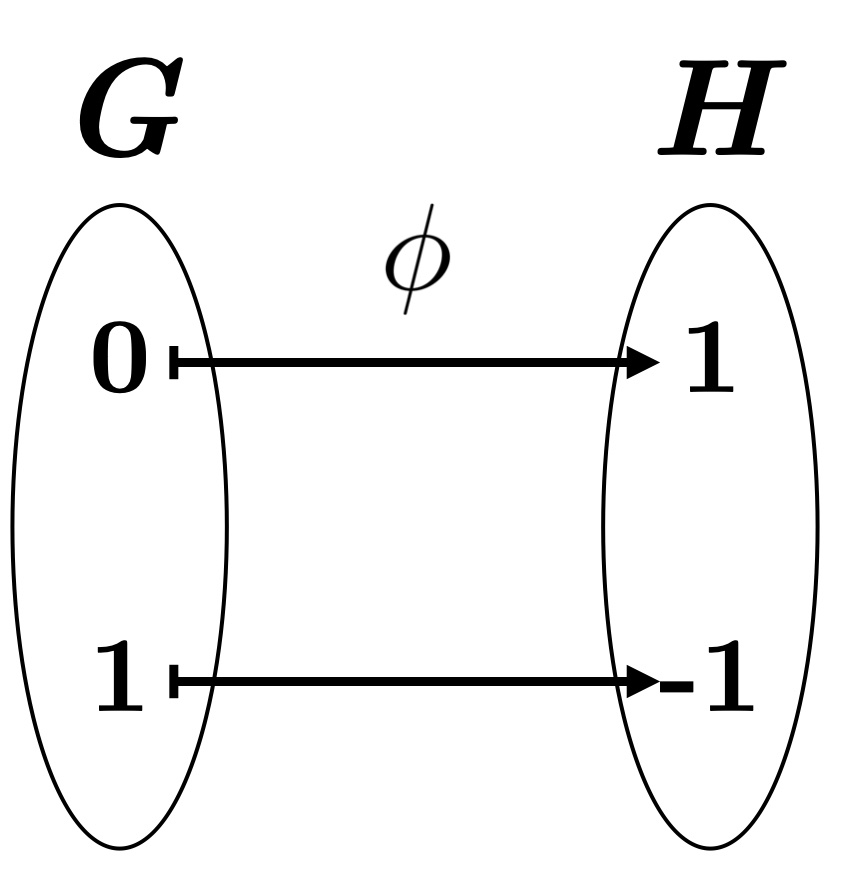
\includegraphics[width=3cm]{images/chapter4/IsomorphismFunctionMap.jpg}}
        \end{figure}
        \item $\phi$ is a homomorphism:\begin{itemize}
            \item $\phi(0\oplus_20) = \phi(0) = 1 = 1 \times 1 = \phi(0)\phi(0)$
            \item $\phi(0 \oplus_2 1) = \phi(1) = -1 = 1 \times (-1) = \phi(0)\phi(1)$
            \item $\phi(1 \oplus_2 0) = \phi(1) = -1 = (-1) \times 1 = \phi(1)\phi(0)$
            \item $\phi(1 \oplus_2 1) = \phi(0) = 1 = (-1) \times (-1) = \phi(1)\phi(1)$
        \end{itemize}
    \end{itemize}
    Thus, $G \cong H$.
\end{example}

\begin{example}
    We show that $(\mathbb{R}, +) \cong ((0, \infty), \times)$ by considering the map $\phi: \mathbb{R} \to (0, \infty), x \mapsto e^x$.
    \begin{itemize}
        \item \textbf{Homomorphism}:
        \[
            \phi(x+y) = e^{x+y} = e^xe^y = \phi(x)\phi(y)
        \]
        \item \textbf{Injective}: Suppose $x$ and $y$ are elements in $\mathbb{R}$ such that $\phi(x) = \phi(y)$. Therefore $e^x = e^y$ which quickly implies $x = y$ by applying natural logarithm ($\ln$) on both sides.
        \item \textbf{Surjective}: Suppose $y \in (0, \infty)$. Then $\ln y$ is a real number. So $\phi(\ln y) = e^{\ln y} = y$, meaning every element in the codomain $(0, \infty)$ has a preimage.
    \end{itemize}

    Thus, $\phi$ is an isomorphism, meaning that $(\mathbb{R}, +) \cong ((0, \infty), \times)$.
\end{example}

\begin{exercise}
    Let the groups $G = (\{1, 2, 3, 4\}, \otimes_5)$ and $H = (\{1, 3, 7, 9\}, \otimes_{10})$.
    \begin{enumerate}[label=(\roman*)]
        \item Show that $G = \langle 3 \rangle$ and $H = \langle 7 \rangle$.
        \item Prove that $G \cong H$ by considering the map $\phi: G \to H, 3^k \mapsto 7^k$.
    \end{enumerate}
\end{exercise}

\section{Consequences of Isomorphisms}
Isomorphisms between groups means that the two groups \textit{share the same structure}, in a manner of speaking. We look at a theorem that showcases the sharing of some of these properties.
\begin{theorem}\label{thrm-isomorphism-consequences}
    Let $\phi: G \to H$ be an isomorphism between the groups $G$ and $H$. Then
    \begin{enumerate}
        \item $|G| = |H|$;
        \item $\phi^{-1}: H \to G$ is an isomorphism;
        \item if $G$ is abelian then so is $H$;
        \item if $G$ is cyclic then so is $H$; and
        \item if $G$ has a subgroup of order $n$, then so does $H$.
    \end{enumerate}
\end{theorem}
\begin{proof}
    We prove each of these statements individually.
    \begin{enumerate}
        \item Follows immediately from properties of a bijective function.

        \item Since $\phi$ is an isomorphism, it is bijective, which means that $\phi^{-1}$ exists and is also bijective. All that remains is to show that $\phi^{-1}$ is a homomorphism.

        Let $u$ and $v$ be in $H$. Then there exist elements $x$ and $y$ in $G$ such that
        \[
            \phi(x) = u \text{ and } \phi(y) = v
        \]
        since $\phi$ is surjective. Hence,
        \begin{align*}
            \phi^{-1}(uv) &= \phi^{-1}\left(\phi(x)\phi(y)\right)\\
            &= \phi^{-1}\left(\phi(xy)\right) & (\text{since } \phi \text{ is a homomorphism})\\
            &= xy\\
            &= \phi^{-1}(u) \phi^{-1}(v).
        \end{align*}
        Thus $\phi^{-1}$ is an isomorphism.

        \item Suppose $u$ and $v$ are in $H$. Let $x$ and $y$ be elements in $G$ such that
        \[
            \phi(x) = u \text{ and } \phi(y) = v.
        \]
        Thus,
        \begin{align*}
            uv = &= \phi(x)\phi(y) \\
            &= \phi(\underbrace{xy}_{\text{In } G})\\
            &= \phi(yx) & (\text{since } G \text{ is abelian})\\
            &= \phi(y)\phi(x)\\
            &= vu
        \end{align*}
        which means that $uv = vu$. Hence $H$ is abelian.

        \item Suppose $u$ is in $H$. Let $x$ be in $G$ such that $\phi(x) = u$. Since $G$ is cyclic, suppose $g$ is the generator of $G$, so $x = g^n$ for some integer $n$. This means that
        \begin{align*}
            u &= \phi(x)\\
            &= \phi(g^n)\\
            &= \underbrace{\phi(g)\phi(g)\phi(g)\cdots\phi(g)}_{n \text{ times}}\\
            &= \left(\phi(g)\right)^n\\
            &\in \left\langle \phi(g) \right\rangle.
        \end{align*}
        Thus any element $u$ in $H$ is in $\left\langle \phi(g) \right\rangle$, meaning $H \subseteq \left\langle \phi(g) \right\rangle$.

        However, $\left\langle \underbrace{\phi(g)}_{\text{In }H} \right\rangle \leq H$ which means that $\left\langle \phi(g) \right\rangle \subseteq H$. Therefore, we have $H \subseteq \left\langle \phi(g) \right\rangle$ and $\left\langle \phi(g) \right\rangle \subseteq H$ simultaneously, meaning $H = \left\langle \phi(g) \right\rangle$, i.e. $H$ is a cyclic group.

        \item Let $K \leq G$ with $|K| = n$. Consider the subgroup $\phi(K)$. By properties of homomorphism, $\phi(K) \leq H = \phi(G)$. Now by property (1), $|K| = |\phi(K)| = n$, meaning that there is a subgroup of $H$ with order $n$, namely the subgroup $\phi(K)$.
    \end{enumerate}

    This proves the theorem.
\end{proof}

\begin{exercise}
    Let $\phi: G \to H$ be an isomorphism between the groups $G$ and $H$. Show that if $G$ has a normal subgroup with order $k$, then $H$ also has a normal subgroup of order $k$.
\end{exercise}

\section{Links to Cyclic Groups}
With the tool of isomorphism under our belt, we can prove two important theorems regarding cyclic groups. Before that, however, we need to introduce the idea of \textbf{infinite cyclic groups}.
\begin{definition}
    An infinite cyclic group $G$ generated by $g$ is denoted by $\langle g \rangle$ and has order $|G| = \infty$. So,
    \[
        G = \{\dots, g^{-2}, g^{-1}, e, g, g^2, \dots\}.
    \]
\end{definition}

For brevity, we also have notation regarding the integers under addition. When we write $\mathbb{Z}_n$, we mean the group $(\mathbb{Z}_n, \oplus_n)$; when we write $\mathbb{Z}$, we mean the group $(\mathbb{Z}, +)$.

\newpage

\begin{theorem}
    If $G = \langle g \rangle$ and $|G| = \infty$, then $G \cong \mathbb{Z}$.
\end{theorem}
\begin{proof}[Proof (see \cite{proofwiki_infinitecyclicgrp}, and {\cite[\S 3.4 Theorem 1]{cohn_1982}})]
    Consider the map $\phi: \mathbb{Z} \to G$ such that $\phi(n) = g^n$. We need to prove that $\phi$ is an isomorphism.
    \begin{itemize}
        \item \textbf{Homomorphism}:
        \[
            \phi(m+n) = g^{m+n} = g^mg^n = \phi(m)\phi(n)
        \]

        \item \textbf{Injective}: Let $m$ and $n$ be integers such that $\phi(m) = \phi(n)$. Without loss of generality, assume that $m \leq n$. Since $\phi(m) = \phi(n)$ we have $g^m = g^n = g^mg^{n-m}$ which implies that $g^{n-m} = e$ by cancellation law.

        If $m < n$, let $k = n - m$. Clearly $k$ is an integer. Thus, $g^k = e$ which means that $|g| = k$. However, $g$ is a generator of $G$, which means that $|g| = |G| = \infty$. Hence, $k = \infty$ which is absurd. Therefore we have a contradiction, meaning $m \not< n$.

        Therefore, $m = n$ which means $k = 0 \implies g^0 = e$ which is valid. Hence, $\phi(m) = \phi(n)$ implies that $m = n$ which proves that $\phi$ is injective.

        \item \textbf{Surjective}: Suppose $x \in G = \langle g\rangle$, so $x = g^n$ for some integer $n$. Then $\phi(n) = g^n = x$ which means that $x$ has a preimage of $n$. Hence $\phi$ is surjective.
    \end{itemize}

    Therefore, $\phi$ is a bijective homomorphism (i.e., isomorphism) which means that $G \cong \mathbb{Z}$.
\end{proof}

\newpage

\begin{theorem}\label{thrm-finite-cyclic-group-isomorphic-to-Zn}
    If $G = \langle g\rangle$ and $|G| = n < \infty$, then $G \cong \mathbb{Z}_n$.
\end{theorem}
\begin{proof}[Proof (cf. {\cite[\S 63]{clark_1984}})]
    Consider $\phi: \mathbb{Z}_n \to G$ such that $\phi(m) = g^m$. We prove that $\phi$ is an isomorphism.
    \begin{itemize}
        \item \textbf{Homomorphism}:
        \[
            \phi(l+m) = g^{l+m} = g^lg^m = \phi(l)\phi(m)
        \]

        \item \textbf{Injective}: Let $l$ and $m$ be integers such that $\phi(l) = \phi(m)$. Without loss of generality, assume that $l \leq m$. Since $\phi(l) = \phi(m)$ we have $g^l = g^m = g^lg^{m-l}$ which implies that $g^{m-l} = e$ by cancellation law.

        If $l < m$ then letting $k = m - l$ means that $k$ belongs to the set $\{1, 2, 3, \dots, n-1\}$. Therefore $g^k = e$ implies that $|g| = k \leq n - 1 < n$. But since $g$ is a generator of $G$, thus $|g| = |G| = n$. Therefore, we have $|g| < n$ and $|g| = n$ simultaneously, a contradiction. Thus $l \not< m$.

        Hence $l = m$, meaning $\phi$ is injective.
        \item \textbf{Surjective}: Suppose $x \in G = \langle g\rangle$, so $x = g^m$ for some integer $m$ in $\mathbb{Z}_n$. Then $\phi(m) = g^m = x$ which means that $x$ has a preimage of $m$. Hence $\phi$ is surjective.
    \end{itemize}

    Therefore, $\phi$ is a bijective homomorphism (isomorphism) which means that $G \cong \mathbb{Z}_n$.
\end{proof}

In summary:
\begin{itemize}
    \item All cyclic groups with \textbf{infinite} order are isomorphic to the group of integers under addition, $\mathbb{Z}$.
    \item All cyclic groups with \textbf{finite} order $n$ are isomorphic to the group of integers under addition modulo $n$, $\mathbb{Z}_n$.
\end{itemize}

\begin{exercise}
    Let $G = (\{1, 3, 7, 9\}, \otimes_{10})$ be a group. Show that $G$ is cyclic and hence find the integer $n$ such that $G \cong \mathbb{Z}_n$.
\end{exercise}

\newpage

\section{Problems}

\begin{problem}
    Let $G$ be a group and $g \in G$. Define the map $f: G \to G, x \mapsto gxg^{-1}$. Prove that $f$ is an isomorphism.
\end{problem}

\begin{problem}
    Let $\mathbb{Q}_{>0}$ denote the set of positive rational numbers. Let $G = (\mathbb{Q}, +)$ and $H = (\mathbb{Q}_{>0}, \times)$ be groups. Prove that $G \not\cong H$.
\end{problem}

\begin{problem}
    Let $G$ and $H$ \textbf{both} be the additive group of integers. Define a map $\phi: G \to H$ such that $\phi(n) = 2n$.
    \begin{enumerate}[label=(\alph*)]
        \item Prove that $\phi$ is a homomorphism.
        \item Prove that $\phi$ is injective.
        \item Prove that there does \textbf{not} exist a homomorphism $\psi: H \to G$ such that $\psi(\phi(n)) = n$.
    \end{enumerate}
\end{problem}

\begin{problem}
    Let $G$ be a group. Define a map $f: G \to G$ such that $f(g) = g^{-1}$ for all $g$ in $G$. Prove that $G$ is abelian if and only if $f$ is a homomorphism.
\end{problem}

\begin{problem}
    Let $G$ and $H$ be groups. Suppose that we have a surjective homomorphism $\phi: G \to H$. Prove that if $G$ is abelian, then so is $H$.
\end{problem}

\begin{problem}
    Let $G$ and $H$ be groups. Suppose that we have a surjective homomorphism $\phi: G \to H$. Let $N \lhd G$. Show that $\phi(N) \lhd H$. (That is, the image of $N$ under $\phi$ is a normal subgroup of $H$.)
\end{problem}

\begin{problem}\label{problem-Zn-isomorphic-to-Z-by-nZ}
    Let $G = (\mathbb{Z}_n, \oplus_n)$, and $H = \mathbb{Z}/(n\mathbb{Z})$ be under addition. Prove that $G \cong H$.
\end{problem}

\begin{problem}\label{problem-subgroup-of-quotient-group-is-quotient-group}
    Let $G$ be a group and $N \lhd G$. Let $B$ be a subgroup of the quotient group $G/N$. Prove that $B = A/N$, where $A$ is a subgroup of $G$ such that $N \subseteq A$.
\end{problem}

%=========================================
\chapter{Cayley's Theorem}
This chapter is central to the relevance and analysis of group theory. Cayley's theorem links our ideas of symmetry with the idea of groups, and how groups are a form of \textit{generalized symmetry}. It answers why group theory is oft called ``the study of symmetry'', and highlights the importance of bijections in our study of groups.

\section{Permutations}
A bijective function is too abstract an object. Such functions can take many forms. Thus, it is worth asking: what properties must a bijective function satisfy?

A bijective function is a function that maps all elements from one set to another set exactly. There are no leftovers (surjective), and each output has exactly one input that produces it (injective). In a sense, a bijective function \textit{rearranges} the elements in a set; it renames elements and shuffles them around, without destroying the relative relationships between the elements.

For bijections between finite groups, each group has the same number of elements, so it is reasonable to talk about the rearrangement and enumeration of elements in such groups.
\begin{itemize}
    \item What we mean by \textbf{rearrange} is to rename elements. We can give elements a new name and place it in the codomain.
    \item What we mean by \textbf{enumeration} is to assign each element in each finite group a unique `index number', per se. Each element can have a unique number identifying its original \textit{position} in the group, and its final position in the destination group.
\end{itemize}

Such bijections between finite groups are called \textbf{permutations}, since they simply permute the `index number' of the elements in the groups.

\begin{example}
    Consider the set $S = \{1, 2, 3, 4, 5\}$. A bijection $f: S \to S$ could perform the following mapping:
    \begin{itemize}
        \item $1 \mapsto 2$
        \item $2 \mapsto 4$
        \item $3 \mapsto 3$
        \item $4 \mapsto 5$
        \item $5 \mapsto 1$
    \end{itemize}
    In this case, the function $f$ is said to be a permutation because the ordered list $[2, 4, 3, 5, 1]$ is one rearrangement of the items in the set $\{1, 2, 3, 4, 5\}$.
\end{example}

\begin{remark}
    It is certainly confusing that the operation of rearranging the items is also called \textit{permuting} the items in the set, and one such rearrangement is called a permutation. In group theory, treat a ``permutation'' as a bijective function between finite groups.
\end{remark}

Permutations come in many different forms, but the core thing that they do is to rearrange items. From the above example, one could form a `cycle' of how each item is mapped to another:
\begin{itemize}
    \item $1 \mapsto 2 \mapsto 4 \mapsto 5 \mapsto 1$
    \item $3 \mapsto 3$
\end{itemize}
We can describe a permutation based on how it cycles elements. Consider this alternate mapping performed by the map $\phi: S \to S$:
\begin{itemize}
    \item $1 \mapsto 2$
    \item $2 \mapsto 4$
    \item $3 \mapsto 5$
    \item $4 \mapsto 1$
    \item $5 \mapsto 3$
\end{itemize}
How $\phi$ operates on an element can be described in \textbf{cycle notation}. Here's how to describe a permutation in cycle notation.
\begin{enumerate}
    \item Start by opening a bracket: ``(''.
    \item Write the first element that has not appeared yet in the cycle notation.
    \begin{itemize}
        \item Initially, we write the number 1, so it currently looks like: ``(1''.
    \end{itemize}
    \item Find out where that element is mapped to.
    \begin{itemize}
        \item For the case of the element 1, it is mapped to 2.
    \end{itemize}
    \item Write the mapped element next to the previous element.
    \begin{itemize}
        \item In this case, we will write ``(1 2''
    \end{itemize}
    \item Repeat previous two steps with the mapped element, until reaching an element that has already appeared in the cycle notation.
    \begin{itemize}
        \item Since 2 maps to 4, we will continue to write: ``(1 2 4''
        \item Since 4 maps to 1, we terminate this process.
    \end{itemize}
    \item Close the bracket.
    \begin{itemize}
        \item So our first cycle looks like ``(1 2 4)''
    \end{itemize}
    \item Repeat above steps until all elements are used.
    \begin{itemize}
        \item So our final cycle notation for $g$ is ``(1 2 4)(3 5)''
    \end{itemize}
\end{enumerate}
Some important things to note about this process:
\begin{itemize}
    \item Omit any elements that maps to itself. For example, if $1 \mapsto 3$, $2 \mapsto 6$, $3 \mapsto 4$, $4 \mapsto 1$, $5 \mapsto 5$, $6 \mapsto 2$, and $7 \mapsto 7$, then the corresponding cycle notation is ``(1 3 4)(2 6)'', ignoring the 5 and 7.
    \item If the permutation is the identity permutation, then it has cycle notation of ``(1)''.
\end{itemize}

\begin{example}
    Consider the permutation $\alpha$ which has cycle notation $\begin{pmatrix}1 & 3 & 5 & 2\end{pmatrix}$. This means that:
    \begin{itemize}
        \item $\alpha(1) = 3$
        \item $\alpha(2) = 1$
        \item $\alpha(3) = 5$
        \item $\alpha(4) = 4$
        \item $\alpha(5) = 2$
        \item $\alpha(n) = n$ for $n \geq 6$
    \end{itemize}
\end{example}

\begin{example}
    Consider the permutation $\beta$ which has cycle notation $\begin{pmatrix}1 & 6 & 2 & 9 & 7 & 4\end{pmatrix}$. This means that:
    \begin{itemize}
        \item $\beta(1) = 6$
        \item $\beta(2) = 9$
        \item $\beta(3) = 3$
        \item $\beta(4) = 1$
        \item $\beta(5) = 5$
        \item $\beta(6) = 2$
        \item $\beta(7) = 4$
        \item $\beta(8) = 8$
        \item $\beta(9) = 7$
        \item $\beta(n) = n$ for $n \geq 10$
    \end{itemize}
\end{example}

\begin{exercise}
    Write the cycle notation for these permutations:
    \begin{enumerate}[label=(\alph*)]
        \item $1 \mapsto 2$, $2 \mapsto 3$, $3 \mapsto 1$
        \item $1 \mapsto 3$, $2 \mapsto 2$, $3 \mapsto 1$
        \item $1 \mapsto 3$, $2 \mapsto 4$, $3 \mapsto 1$, $4 \mapsto 5$, $5 \mapsto 2$
    \end{enumerate}
\end{exercise}

We now look at composing permutations.
\begin{example}
    Let $f$ and $g$ be permutations. Let $f$ have cycle notation $\begin{pmatrix}1 & 3 & 5 & 2\end{pmatrix}$ and $g$ have cycle notation $\begin{pmatrix}2 & 4 & 3\end{pmatrix}$. Then $h = fg$ is a permutation with:
    \begin{itemize}
        \item $h(1) = f(g(1)) = f(1) = 3$
        \item $h(2) = f(g(2)) = f(4) = 4$
        \item $h(3) = f(g(3)) = f(2) = 1$
        \item $h(4) = f(g(4)) = f(3) = 5$
        \item $h(5) = f(g(5)) = f(5) = 2$
    \end{itemize}

    So $h$:
    \begin{itemize}
        \item $1 \mapsto 3$
        \item $2 \mapsto 4$
        \item $3 \mapsto 1$
        \item $4 \mapsto 5$
        \item $5 \mapsto 2$
    \end{itemize}
    and thus $h$ has cycle notation $\begin{pmatrix}1 & 3\end{pmatrix}\begin{pmatrix}2 & 4 & 5\end{pmatrix}$.
\end{example}

\begin{example}
    Consider $\begin{pmatrix}2 & 9 & 7 & 4\end{pmatrix}\begin{pmatrix}1 & 6 & 4\end{pmatrix}$. Then:
    \[\begin{pmatrix}2 & 9 & 7 & 4\end{pmatrix}\begin{pmatrix}1 & 6 & 4\end{pmatrix} = \begin{pmatrix}1 & 6 & 2 & 9 & 7 & 4\end{pmatrix}.\]
\end{example}

We now consider how to find the inverse of a permutation. Given a cycle notation for the permutation $f$, simply read the cycle notation backwards, ensuring that the smallest element remains at the front.

\begin{example}
    $\begin{pmatrix}1 & 8 & 4 & 2\end{pmatrix}^{-1} = \begin{pmatrix}2 & 4 & 8 & 1\end{pmatrix} = \begin{pmatrix}1 & 2 & 4 & 8\end{pmatrix}$.
\end{example}

\begin{example}
    $\begin{pmatrix}1 & 7 & 5 & 3 & 9\end{pmatrix}^{-1} = \begin{pmatrix}1 & 9 & 3 & 5 & 7\end{pmatrix}$.
\end{example}

\begin{exercise}
    Find the inverse of the permutation $\pi$, which has cycle notation
    \[
        \begin{pmatrix}1 & 5 & 2\end{pmatrix}\begin{pmatrix}2 & 5 & 3 & 4\end{pmatrix}.
    \]
\end{exercise}

\section{The Symmetric Group of a Set}
With the definition of permutations out of the way, we can finally introduce a very important type of group: the \textbf{symmetric group} of a set $X$.

\begin{definition}
    Let $X$ be a set. Define
    \[
        \Sym{X} = \{f: X \to X \ | \ f \text{ is a bijection}\}.
    \]
\end{definition}
\begin{proposition}
    $(\Sym{X}, \circ)$ is a group, where $\circ$ is the function composition operator.
\end{proposition}
\begin{proof}
    We prove the 4 group axioms.
    \begin{enumerate}
        \item \textbf{Closure}: Let $f$ and $g$ be functions in $\Sym{X}$, so $f: X\to X$ and $g:X \to X$ are bijective functions. Define $h:X \to X$ where $h = f\circ g$. We show that $h$ is bijective:
        \begin{itemize}
            \item \textbf{Injective}: Let $x$ and $y$ be elements in $X$ such that $h(x) = h(y)$. Then:
            \begin{align*}
                f(g(x)) &= f(g(y)) & (\text{by definition of } h)\\
                g(x) &= g(y) & (\text{since } f \text{ is bijective})\\
                x &= y & (\text{since } g \text{ is bijective})
            \end{align*}
            Therefore $h(x) = h(y)$ implies $x = y$.
            \item \textbf{Surjective}: Let $y$ be an element in $X$. Note that since $f$ and $g$ are bijective, therefore $f^{-1}(y)$ is in $X$ and so is $g^{-1}(f^{-1}(y))$. Note also that
            \[
                h(g^{-1}(f^{-1}(y))) = f(g(g^{-1}(f^{-1}(y)))) = y
            \]
            so a preimage of $y$ exists in the domain, meaning that $h$ is surjective.
        \end{itemize}
        Since $h$ is injective and surjective, it is hence bijective. Thus $\Sym{X}$ is closed under $\circ$.
        \item \textbf{Associativity}: Function composition is associative.
        \item \textbf{Identity}: Let $\id : X \to X$ be such that $\id(x) = x$. Clearly $\id$ is in $\Sym{X}$:
        \begin{itemize}
            \item \textbf{Injective}: If $x$ and $y$ are in $X$ such that $\id(x) = \id(y)$ then clearly $x = y$.
            \item \textbf{Surjective}: Let $y$ be in $X$. Since $\id(y) = y$ thus $y$ is its own pre-image under $\id$.
        \end{itemize}
        Now we show that $\id$ is indeed the identity in $\Sym{X}$. Let $x$ be an arbitrary element of $X$, and $f$ be any function in $\Sym{X}$. Then:
        \[
            (\id \circ f)(x) = \id(f(x)) = f(x)
        \]
        and
        \[
            (f \circ \id)(x) = f(\id(x)) = f(x)
        \]
        so $\id$ is the identity in $\Sym{X}$.
        \item \textbf{Inverse}: For all functions $f$ in $\Sym{X}$, $f^{-1}$ exists since $f$ is a bijection. Furthermore, $f^{-1}$ is a bijection from $X$ to $X$, so $f^{-1}$ is in $\Sym{X}$. By definition of $f^{-1}$,
        \[
            f \circ f^{-1} = f^{-1} \circ f = \id
        \]
        so $f^{-1}$ is indeed the inverse of $f$ in $\Sym{X}$.
    \end{enumerate}
    Therefore $(\Sym{X}, \circ)$ is a group.
\end{proof}

The group $(\Sym{X}, \circ)$ is called the \textbf{symmetric group} of $X$. We usually suppress the function composition operator and call $\Sym{X}$ the symmetric group of $X$.

The most relevant type of symmetric group we encounter when working with finite groups is the \textbf{symmetric group of degree $n$} (or symmetric group of $n$ letters).
\begin{definition}
    The \textbf{symmetric group of degree $n$} is denoted by $\Sn{n}$ and is equal to $\Sym{\{1, 2, 3, \dots, n\}}$.
\end{definition}

Let's look at a specific example of a symmetric group of degree $n$.
\begin{example}\label{example-symmetric-group-of-degree-3}
    Consider the symmetric group of degree 3, $\Sn{3}$. We show all function mappings of $\Sn{3}$.

    \begin{figure}[h]
        \centering
        \fbox{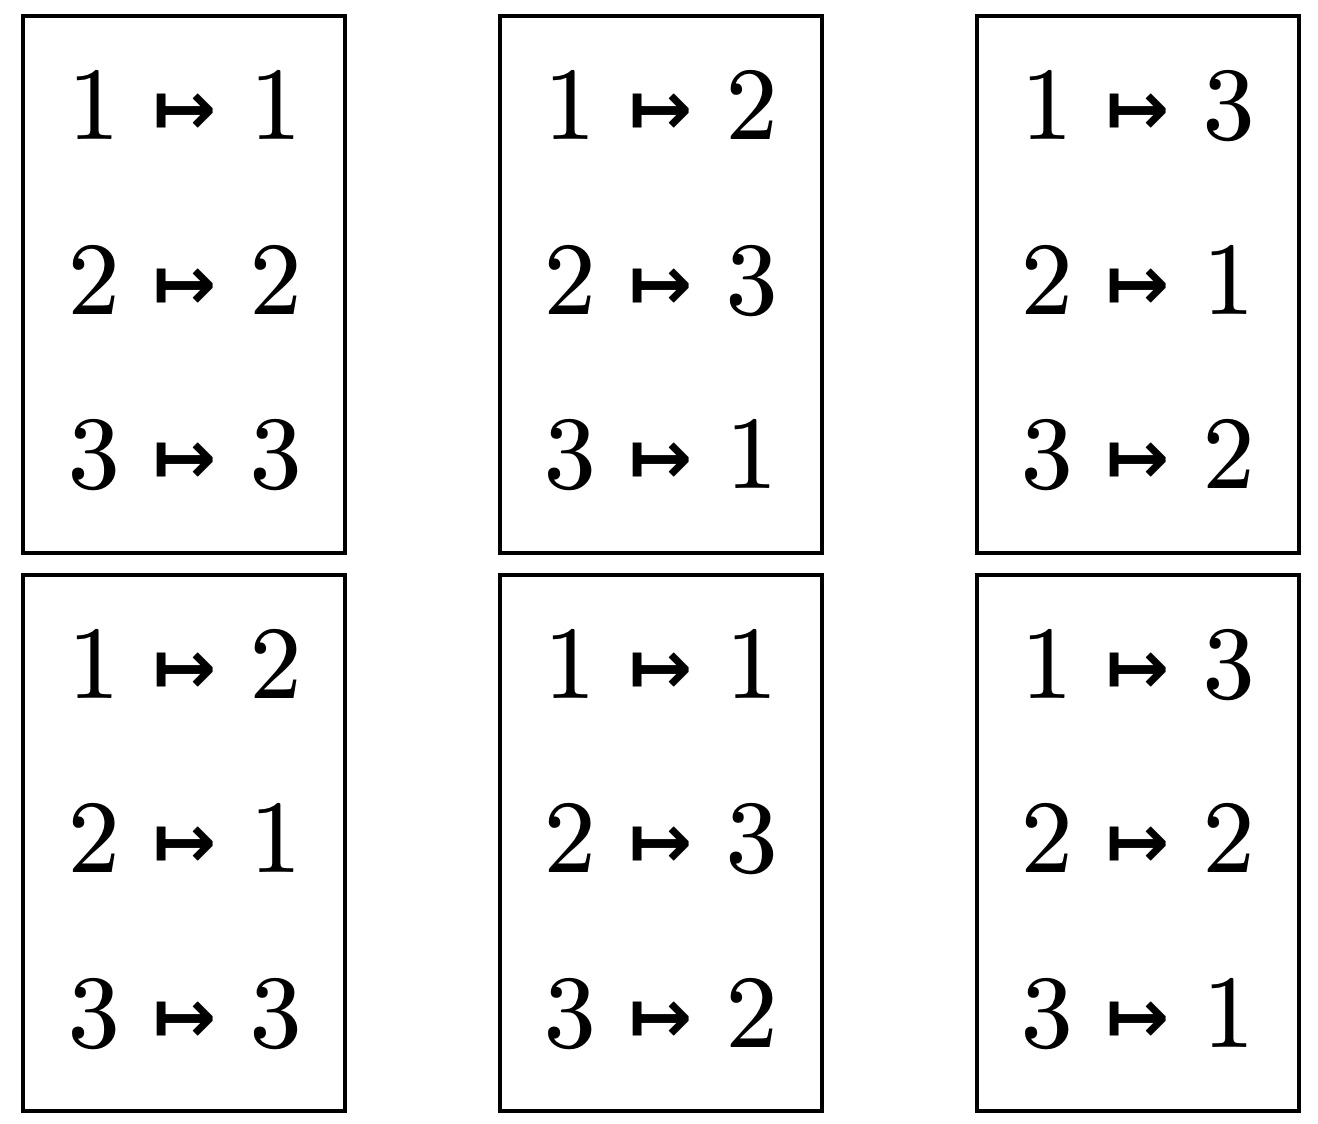
\includegraphics[width=5cm]{images/chapter5/MappingsOfS3.jpg}}
        \caption{All Mappings of $\Sn{3}$}
    \end{figure}

    Thus, $|\Sn{3}| = 6$.
\end{example}
\begin{exercise}\label{exercise-order-of-Sn}
    Explain why $|\Sn{n}| = n!$.
\end{exercise}

\begin{remark}
    Elements of $\Sn{n}$ are called permutations.
\end{remark}

It should also be noted that subgroups of $\Sym{X}$ (where $X$ is any set) are called \textbf{permutation groups}, primarily because they contain permutations. Since a group is its own subgroup, the symmetric group may sometimes be called \textit{the} permutation group.

Finally, we prove one important proposition regarding the symmetric group of a finite set and the symmetric group of a certain degree.
\begin{proposition}\label{prop-symmetric-group-of-finite-order}
    $\Sym{G} \cong \Sn{n}$ if $G$ is finite with order $n$.
\end{proposition}
\begin{proof}
    Since $G$ has $n$ elements, we can index them. Thus, let the set $G = \{x_1, x_2, \dots, x_n\}$.

    For brevity let $\sigma$ denote an arbitrary permutation in $\Sn{n}$. Let the map $\phi: \Sn{n} \to \Sym{G}$ be defined such that $\left(\phi(\sigma)\right)(x_i) = x_{\sigma(i)}$ for all $\sigma$ in $\Sn{n}$ and $x_i$ in $G$. We need to show that $\phi$ is an isomorphism.
    \begin{itemize}
        \item \textbf{Homomorphism}: Let $\sigma$ and $\pi$ be permutations in $\Sn{n}$. Let $x_i$ be an element of $G$. Then
        \begin{align*}
            \left(\phi(\sigma \pi)\right)(x_i) &= x_{\sigma(\pi(i))}\\
            &= \left(\phi(\sigma)\right)\left(x_{\pi(i)}\right)\\
            &= \left(\left(\phi(\sigma)\right)\left(\phi(\pi)\right)\right)(x_i)
        \end{align*}
        which means that $\phi$ is a homomorphism.

        \item \textbf{Injective}: Let $\sigma$ and $\pi$ be permutations in $\Sn{n}$ such that $\phi(\sigma) = \phi(\pi)$, i.e. for all $x_i$ in $G$, we have
        \[
            x_{\sigma(i)} = \left(\phi(\sigma)\right)(x_i) = \left(\phi(\pi)\right)(x_i) = x_{\pi(i)}.
        \]
        Therefore $x_{\sigma(i)} = x_{\pi(i)}$. Now each element of $G$ is uniquely indexed. Thus if two elements are equal, they have to have the same index. Hence, $\sigma(i) = \pi(i)$, for all \textit{valid} $i$. This means $\sigma = \pi$ which proves that $\phi$ is injective.

        \item \textbf{Surjective}: Since $|\Sym{G}| = |G|! = n! = |\Sn{n}|$ by \textbf{Exercise \ref{exercise-order-of-Sn}}, thus $\phi$ is surjective.
    \end{itemize}

    Therefore there exists an isomorphism $\phi$ from $\Sn{n}$ to $\Sym{G}$, meaning that $\Sym{G} \cong \Sn{n}$.
\end{proof}

\newpage

\section{Cayley's Theorem}
We now have sufficient background to state and prove Cayley's theorem.

\begin{theorem}[Cayley]\label{thrm-cayley}
    Every group is isomorphic to a permutation group.
\end{theorem}

The statement of the theorem, although simple, is the reason \textit{why} group theorists study group theory: to explore all the ways that a group can be symmetric.

The proof of this theorem is involved and technical, but we'll try and simplify its proof as much as possible.

\begin{proof}
    Let $G$ be any group. We want to prove that there exists a group of bijective functions from $G$ to $G$ that is isomorphic to $G$ (i.e., a permutation group).

    For any $g$ in $G$ define the map $\lambda_g: G \to G$ such that $x \mapsto gx$. We claim that $\lambda_g$ is a bijection.
    \begin{itemize}
        \item \textbf{Injective}: Let $x$ and $y$ be elements of $G$ such that $\lambda_g(x) = \lambda_g(y)$. Then $gx = gy$ by definition of $\lambda_g$ which immediately means $x = y$ by group cancellation law. Thus $\lambda_g(x) = \lambda_g(y)$ implies $x = y$, meaning $\lambda_g$ is injective.
        
        \item \textbf{Surjective}: Let $y$ be an element of $G$. Note that $g^{-1}y$ is an element of $G$ (since $G$ is closed), and that $\lambda_g(g^{-1}y) = g(g^{-1}y) = y$. Thus, a preimage of $y$ is $g^{-1}y$ and it exists in the domain $G$, meaning $\lambda_g$ is surjective.
    \end{itemize}
    Since $\lambda_g$ is both injective and surjective it is thus bijective.

    Now let $H = \{\lambda_g \ | \ g \in G\}$. Since $\lambda_g$ is a bijective function from $G$ to $G$, it thus is an element of $\Sym{X}$, meaning that $H \subseteq \Sym{G}$. It remains to show that $H \leq \Sym{G}$. We do this by using the subgroup test.

    We first note that $\lambda_e = \id$ since
    \[
        \lambda_e(x) = ex = x = \id(x)
    \]
    for all $x$ in $G$. Also, the inverse of any function $\lambda_g$ is $\lambda_{g^{-1}}$ since
    \[
        \lambda_g \circ \lambda_{g^{-1}}(x) = gg^{-1}x = x = \lambda_e(x)
    \]
    and
    \[
        \lambda_{g^{-1}} \circ \lambda_g(x) = g^{-1}gx = x = \lambda_e(x).
    \]
    Now suppose $\lambda_{g_1}, \lambda_{g_2} \in H$ (where $g_1, g_2 \in G$). Note $g_1g_2^{-1}$ is an element of $G$ since $G$ is closed. Therefore, for all $x$ in $G$,
    \begin{align*}
        \lambda_{g_1} \circ \left(\lambda_{g_2}\right)^{-1}(x) &= \lambda_{g_1}\circ\lambda_{g_2^{-1}}(x)\\
        &= g_1g_2^{-1}x\\
        &= \lambda_{g_1g_2^{-1}}(x)
    \end{align*}
    which is clearly an element of $H$. Thus if $\lambda_{g_1}$ and $\lambda_{g_2}$ are functions in $H$, then $\lambda_{g_1} \circ \left(\lambda_{g_2}\right)^{-1}$ is also a function in $H$. Since $H$ is non-empty, therefore by the Subgroup Test, we have shown $H \leq \Sym{G}$.

    We finally show that $G \cong H$ by considering the map $\phi: G\to H, g \mapsto \lambda_g$. We need to show that $\phi$ is an isomorphism:
    \begin{itemize}
        \item \textbf{Homomorphism}: For any $x$ in $G$,
            \begin{align*}
                \phi(gh)(x) &= \lambda_{gh}(x)\\
                &= ghx\\
                &= g(hx)\\
                &= \lambda_g\left(\lambda_h(x)\right)\\
                &= \lambda_g\circ\lambda_h(x)\\
                &= (\phi(g)\phi(h))(x).
            \end{align*}
            Thus, $\phi(gh) = \phi(g)\phi(h)$.
        
        \item \textbf{Injective}: Let $g_1$ and $g_2$ be elements in $G$ such that $\phi(g_1) = \phi(g_2)$. Then $\lambda_{g_1} = \lambda_{g_2}$. Therefore, $\lambda_{g_1}(x) = \lambda_{g_2}(x)$ for all $x$ in $G$, which means that $\lambda_{g_1}(e) = \lambda_{g_2}(e)$ when $x = e$. By definition of $\lambda_g$, we have $eg_1 = eg_2$ which ultimately means that $g_1=g_2$. Thus if $\phi(g_1) = \phi(g_2)$ then $g_1=g_2$.
        
        \item \textbf{Surjective}: The number of functions in $H$ equals the number of elements of $G$ by definition of $H$. Thus, since $\phi$ is surjective.
    \end{itemize}
    Therefore we have proven that $\phi$ is an isomorphism, which means that $G \cong H \leq \Sym{G}$, that is, any group $G$ is isomorphic to a subgroup of the symmetric group of $G$ (i.e., a permutation group).
\end{proof}

We note one corollary of this theorem.
\begin{corollary-thrm}
    Let $G$ be a finite group of order $n$. Then there exists a group $H \leq \Sn{n}$ such that $G \cong H$.
\end{corollary-thrm}
\begin{proof}
    By Cayley's theorem (\textbf{Theorem \ref{thrm-cayley}}), there exists a group $H \leq \Sym{G}$ such that $G \cong H$. Now since $G$ is finite with order $n$, thus by \textbf{Proposition \ref{prop-symmetric-group-of-finite-order}}, $\Sym{G} \cong \Sn{n}$. Thus, $H \leq \Sn{n}$, and $G \cong H$.
\end{proof}

One might ask what the use of Cayley's Theorem is in group theory. To put it simply, it is a sanity check on the definition of a group. Before anyone had the idea of writing down the axioms for groups, people studied collections of bijections of sets closed under composition and inverses. Cayley's Theorem tells us that every abstract group is a type of the above collection, so the axioms of group theory capture the concrete phenomenon that groups were designed to capture.

\newpage

\section{Problems}
\begin{problem}
    Let the permutations
    \begin{align*}
        &\alpha = \begin{pmatrix}1 & 5 & 2 & 3\end{pmatrix},\\
        &\beta  = \begin{pmatrix}1 & 5 & 2\end{pmatrix}\begin{pmatrix}3 & 4\end{pmatrix},\\
        &\gamma = \begin{pmatrix}1 & 2 & 5\end{pmatrix}\begin{pmatrix}3 & 4\end{pmatrix}, \text{ and}\\
        &\delta = \begin{pmatrix}1 & 3 & 2 & 5\end{pmatrix}.
    \end{align*}
    What is the cycle notation of the permutation $\alpha\beta\gamma\delta$?
\end{problem}

\begin{problem}
    Prove that the symmetric group of degree 3, $\Sn{3}$, is isomorphic to the dihedral group of order 6, $D_3$.
\end{problem}

\begin{problem}
    State the number of elements in $\Sn{4}$.
    \begin{enumerate}[label=(\alph*)]
        \item Let $G$ be the cyclic group of order 4. Cayley’s Theorem says that it is isomorphic to a subgroup of $\Sn{4}$. Find one such subgroup and prove that it is, indeed, isomorphic to $G$.
        \item Let $G$ be the group with presentation
        \[
            \langle a, b \ | \ a^2 = b^2 = (ab)^2 = e \rangle.
        \]
        Cayley’s Theorem says that it is isomorphic to a subgroup of $\Sn{4}$. Find one such subgroup and prove that it is, indeed, isomorphic to $G$.
    \end{enumerate}
\end{problem}

%=========================================
\chapter{Direct Products of Groups}
\section{External Direct Product}
The external direct product is one method of `combining' groups together.
\begin{definition}
    Let $(G, \ast)$ and $(H, \star)$ be groups. The \textbf{external direct product} of $G$ and $H$ is denoted by $G\times H$ and is the group $(G\times H, (\ast, \star))$, where $G\times H$ is the Cartesian product of $G$ and $H$, and $(\ast, \star)$ are the operators performed component-wise.
\end{definition}
Note that $|G \times H| = |G||H|$ by definition of the Cartesian product.

\begin{example}
    $\mathbb{Z}_5 \times \mathbb{Z} = \{(m,n) \ | \ m \in \mathbb{Z}_5 \text{ and } n \in \mathbb{Z}\}$.

    Thus, $(2, 5)(5, 9) = (2 \oplus_5 5, 5 + 9) = (2, 14)$.
\end{example}

\begin{example}
    Let $\mathcal{S} = \mathbb{R}\setminus\{0\}$ be a group under multiplication. Then $\mathcal{S} \times \mathbb{Z}_3 = \{ (x, n) \ | \ x \in \mathcal{S} \text{ and } n \in \mathbb{Z}_3\}$.

    So, $(3, 2)^{-1} = \left(\frac13, 1\right)$ since
    \begin{align*}
        (3, 2)\left(\frac13, 1\right) &= \left(3 \times \frac13, 2 \oplus_3 1\right)\\
        &= (1, 0)\\
        &= (\text{Identity in }\mathcal{S}, \text{Identity in }\mathbb{Z}_3)
    \end{align*}
\end{example}

\begin{exercise}
    What is $(s, rs)(r^2s, r^3)$ in the group $D_3 \times D_4$?
\end{exercise}

\newpage

We prove some results relating the external direct product.
\begin{proposition}\label{prop-order-of-element-in-external-direct-product}
    Let $G_1$ and $G_2$ be groups with identities $e_1$ and $e_2$ respectively. Let $(x, y) \in G_1 \times G_2$, $|x| = r$, $|y| = s$, and $e_{1,2}$ be the identity of $G_1\times G_2$. Then $|(x, y)| = \lcm(r, s)$.
\end{proposition}
\begin{proof}[Proof (see \cite{proofwiki_orderofgroupelementinexternaldirectproduct})]
    For brevity let $l = \lcm(r, s)$, so $l = \alpha r = \beta s$ for some positive integers $\alpha$ and $\beta$. Let $m = |(x, y)|$.

    Note that
    \begin{align*}
        (x, y)^l &= (x^l, y^l)\\
        &= (x^{\alpha r}, y^{\beta s})\\
        &= \left((x^r)^\alpha, (y^s)^\beta\right)\\
        &= (e_1^\alpha, e_2^\beta)\\
        &= (e_1, e_2)\\
        &= e_{1,2}.
    \end{align*}
    Therefore $l = k|(x, y)| = km$ for some positive integer $k$, i.e. $m | l$.

    Note also that $(x, y)^m = (x^m, y^m)$ and $(x, y)^m = e_{1,2} = (e_1, e_2)$. Therefore $x^m = e_1$ and $y^m = e_2$. Hence,
    \[
        m = p|x| = pr \text{ and } m = q|y| = qs
    \]
    for some positive integers $p$ and $q$, meaning that $r$ and $s$ both divide $m$. Therefore $\lcm(r, s) = l | m$.

    Since $m | l$ and $l | m$, thus $m = l$, meaning $|(x, y)| = \lcm(|x|, |y|)$.
\end{proof}

\begin{theorem}\label{thrm-Zm-cross-Zn-isomorphic-to-Zmn-condition}
    $\mathbb{Z}_m \times \mathbb{Z}_n \cong \mathbb{Z}_{mn}$ if and only if $\gcd(m,n) = 1$.
\end{theorem}
\begin{proof}[Proof (see {\cite[Proposition 13.1 (3)]{humphreys_1996}})]
    We prove the forward direction first. Suppose $\mathbb{Z}_m \times \mathbb{Z}_n \cong \mathbb{Z}_{mn}$. For brevity let $d = \gcd(m,n)$. Suppose on the contrary that $d > 1$.

    Take $(a, b) \in \mathbb{Z}_m \times \mathbb{Z}_n$. Note that $\frac{mn}{d} = \lcm(m,n)$ which is a positive integer. Then
    \begin{align*}
        \underbrace{(a,b)(a,b)(a,b)\cdots(a,b)}_{\frac{mn}{d}\text{ times}} &= \left(\frac{mn}{d}a, \frac{mn}{d}b\right)\\
        &= \left(m\frac{na}{d}, n\frac{mb}{d}\right) & (\text{since } d | m \text{ and } d | n)\\
        &= (\underbrace{0}_{\text{In } \mathbb{Z}_m}, \underbrace{0}_{\text{In } \mathbb{Z}_n})
    \end{align*}
    which implies $|(a, b)| \leq \underbrace{\frac{mn}{d} < mn}_{\text{Since } d > 1}$ for all $(a, b) \in \mathbb{Z}_m \times \mathbb{Z}_n$. Hence, this means that $\mathbb{Z}_m \times \mathbb{Z}_n$ is \textit{not} cyclic, since $|\mathbb{Z}_m \times \mathbb{Z}_n| = mn$ and no element in $\mathbb{Z}_m \times \mathbb{Z}_n$ has order $mn$.

    However, $\mathbb{Z}_m \times \mathbb{Z}_n \cong \mathbb{Z}_{mn}$ which is cyclic, a clear contradiction. Hence, $d \not>1 \implies d = 1$, meaning $\gcd(m,n) = 1$.

    We now work on the reverse direction. Suppose $\gcd(m,n) = 1$. Note that $|1| = m$ in $\mathbb{Z}_m$ and $|1| = n$ in $\mathbb{Z}_n$. Thus
    \begin{align*}
        |(1, 1)| &= \lcm(m, n) & (\text{\textbf{Proposition \ref{prop-order-of-element-in-external-direct-product}}})\\
        &= \frac{mn}{\gcd(m,n)}\\
        &= mn & (\text{since }\gcd(m,n) = 1).
    \end{align*}
    Since $|\mathbb{Z}_m \times \mathbb{Z}_n| = mn$ and $|(1,1)| = mn$, thus $\mathbb{Z}_m \times \mathbb{Z}_n$ is cyclic. By \textbf{Theorem \ref{thrm-finite-cyclic-group-isomorphic-to-Zn}}, $\mathbb{Z}_m \times \mathbb{Z}_n \cong \mathbb{Z}_{mn}$.

    This proves the theorem.
\end{proof}

\begin{exercise}
    Find all pairs of integers $(m, n)$ with $1 < m < n$ such that $\mathbb{Z}_m \times \mathbb{Z}_n \cong \mathbb{Z}_{180}$.
\end{exercise}

\section{Internal Direct Product}
Before we look at the internal direct product, we look at the \textbf{subgroup product}.
\begin{definition}
    Let $G$ be a group and $H, K \leq G$. Then
    \[
        HK = \{hk \ | \ h \in H, k \in K\}
    \]
    is called the \textbf{subgroup product of $H$ and $K$}.
\end{definition}

\begin{proposition}\label{prop-subgroup-product-is-subgroup}
    Let $G$ be a group and $H, K \leq G$. Then $HK \leq G$ if and only if $HK = KH$.
\end{proposition}
\begin{proof}
    We first prove the forward direction; assume that $HK \leq G$. First take an arbitrary $kh \in KH$. Then we note
    \begin{align*}
        kh &= \left(\left(kh\right)^{-1}\right)^{-1}\\
        &= (\underbrace{h^{-1}}_{\text{In } H}\underbrace{k^{-1}}_{\text{In } K})^{-1}\\
        &\in HK
    \end{align*}
    since $HK \leq G$ so the inverse of any element is in $HK$. Therefore any element in $KH$ is also in $HK$, meaning that $KH \subseteq HK$. Now take an arbitrary $hk \in HK$. Note that $k^{-1}h^{-1} = (hk)^{-1} \in HK$, so set $k^{-1}h^{-1} = \hat{h}\hat{k}$ for some $\hat{h} \in H$ and $\hat{k} \in K$. Hence $hk = \left(k^{-1}h^{-1}\right)^{-1} = \hat{k}^{-1}\hat{h}^{-1} \in KH$, meaning $HK \subseteq KH$. Therefore $HK = KH$ as needed.

    We now prove the reverse direction; assume that $HK = KH$. Clearly $e \in HK$ since $e \in H$ and $e \in K$. Now suppose $h_1k_1, h_2k_2 \in HK$. We note
    \begin{align*}
        (h_1k_1)(h_2k_2)^{-1} &= h_1k_1k_2^{-1}h_2^{-1}\\
        &= h_1(\underbrace{k_1k_2^{-1}h_2^{-1}}_{\text{In } KH = HK})\\
        &= h_1(h'k') & (\text{set }(k_1k_2^{-1})h_2^{-1} = h'k')\\
        &= (\underbrace{h_1h'}_{\text{In } H})k'\\
        &\in HK
    \end{align*}
    so by subgroup test, $HK \leq G$.
\end{proof}
An important point to note is that $HK = KH$ does not imply that $hk = kh$ for all $h \in H$ and $k \in K$. Finding a counterexample to this claim is left as an exercise to the reader.

We now look at the \textbf{internal direct product}, another way of combining elements of two groups.

\begin{definition}
    Let $G$ be a group and $H, K \leq G$ such that
    \begin{enumerate}
        \item $G = HK$,
        \item $H \cap K = \{e\}$, and
        \item for all $h \in H$ and $k \in K$, $hk = kh$.
    \end{enumerate}
    Then $G$ is said to be the \textbf{internal direct product} of $H$ and $K$.
\end{definition}

\begin{example}
    Consider $G = D_6$, $H = \langle r^3 \rangle$ and $K = \langle s, r^2 \rangle$. Note that
    \begin{align*}
        HK &= \{hk \ | \ h \in H, k \in K\}\\
        &= \{e, r^2, r^4, s, r^2s, r^4s, r^3, r^5, r^7, r^3s, r^5s, r^7s\}\\
        &= \{e, r^2, r^4, s, r^2s, r^4s, r^3, r^5, r, r^3s, r^5s, rs\}\\
        &= D_6\\
        &= G
    \end{align*}
    so $G = HK$. Note also that $hk = kh$ for all $h$ in $H$ and $k$ in $K$. Thus $G$ is indeed the internal direct product of $H$ and $K$.
\end{example}

\begin{exercise}
    Let $G = \{1, 5\}$ and $H = \{1, 7\}$ be groups under $\otimes_{12}$. Find the internal direct product of $G$ and $H$.
\end{exercise}

\section{The Isomorphism Between Them}
It is certainly tiring to remember that there is an \textit{external} direct product and an \textit{internal} direct product. One might rightly wonder whether we can simplify both into one unified ``direct product''. In fact, there exists and isomorphism between the external direct product and the internal direct product of two groups.

\begin{theorem}\label{thrm-direct-product-equivilance}
    If $G$ is the internal direct product of $H$ and $K$ then $G \cong H \times K$.
\end{theorem}
\begin{proof}
    Let $\phi: G \to H \times K$, $g \mapsto (h, k)$ where $g = hk$. We will show that $\phi$ is a well-defined isomorphism.
    \begin{itemize}
        \item \textbf{Well-defined}: Suppose $g = hk = h'k'$ where $h, h' \in H$ and $k, k' \in K$. Since $hk = h'k'$ thus $h^{-1}h' = k(k')^{-1}$.

        Note that $h^{-1}h' \in H$ and $k(k')^{-1} \in K$. So if $h^{-1}h' = k(k')^{-1}$ then $h^{-1}h' \in H \cap K$ and $k(k')^{-1} \in H \cap K$. But $H \cap K = \{e\}$. So $h^{-1}h' = e \implies h = h'$ and $k(k')^{-1} = e \implies k = k'$. Thus if $g = hk = h'k'$ then $h = h'$ and $k = k'$.
        
        \newpage
        
        \item \textbf{Homomorphism}: Let $g, g' \in G$, $h, h' \in H$, and $k, k' \in K$ such that $g = hk$ and $g' = h'k'$. Then
        \begin{align*}
            \phi(gg') &= \phi(hkh'k')\\
            &= \phi(h(kh')k')\\
            &= \phi(h(h'k)k') & (hk = kh \text{ for all } h \text{ and } k)\\
            &= \phi(\underbrace{hh'}_{\text{In }H}\underbrace{kk'}_{\text{In }K})\\
            &= (hh', kk') & (\text{by definition of }\phi)\\
            &= (h,k)(h',k')\\
            &= \phi(hk)\phi(h'k')\\
            &= \phi(g)\phi(g')
        \end{align*}
        
        \item \textbf{Injective}: Let $g, g' \in G$, $h, h' \in H$, and $k, k' \in K$ such that $g = hk$, $g' = h'k'$, and $\phi(g) = \phi(g')$. Then $\phi(hk) = \phi(h'k')$, meaning $(h,k) = (h',k')$. Thus $h = h'$ and $k = k'$ by equality of ordered pairs, meaning $g = hk = h'k' = g'$.
        
        \item \textbf{Surjective}: Let $(h, k) \in H \times K$. Note that $hk \in G$ since $G$ is the internal direct product of $H$ and $K$, so $\phi(hk) = (h, k)$. Thus a pre-image of $(h, k)$ is $hk$.
    \end{itemize}
    Therefore $\phi$ is a well-defined isomorphism from $G$ to $H \times K$, meaning $G \cong H \times K$.
\end{proof}

\begin{example}
    Consider again $G = D_6$, $H = \langle r^3 \rangle$ and $K = \langle s, r^2 \rangle$. As we have found before, $G = HK$; but we now know that $G \cong H \times K$.

    Note that $|H| = 2$ so $H \cong \mathbb{Z}_2$ and $K \cong D_3$ (we leave the latter as an exercise for the reader to prove). Thus,
    \[
        D_6 = G = HK \cong H \times K = \mathbb{Z}_2 \times D_3.
    \]
\end{example}

\begin{exercise}
    Let $\mathcal{S} = \{1, 5, 7, 11\}$, $G = \{1, 5\}$ and $H = \{1, 7\}$ be groups under $\otimes_{12}$. Find the value of $n$ such that $\mathcal{S} \cong (\mathbb{Z}_n)^2$.
\end{exercise}

\section{Problems}
\begin{problem}\label{problem-external-direct-product-of-abelian-groups-is-abelian}
    Let $G$ and $H$ be abelian groups. Prove that $G \times H$ is also an abelian group.
\end{problem}

\begin{problem}
    Let $G$ and $H$ be groups. Prove that $G \times H \cong H \times G$.
\end{problem}

\begin{problem}
    Let $G = \mathbb{Z}_6$, $H = \{0, 2, 4\}$, and $K = \{0, 3\}$. Determine if $G$ is the internal direct product of $H$ and $K$.
\end{problem}

\begin{problem}
    Consider the \textit{Klein four-group} $\mathrm{V}$ with presentation
    \[
        \langle a, b \ | \ a^2 = b^2 = (ab)^2 = e \rangle.
    \]
    Show that $\mathrm{V} \cong (\mathbb{Z}_2)^2$.
\end{problem}

%=========================================
\chapter{Further Properties of Homomorphisms}
\section{Image of a Homomorphism}
As a homomorphism is a mapping between two groups, it is worthy to look at the image (or range) of the homomorphism.
\begin{definition}
    The \textbf{image} (or \textbf{range}) of a homomorphism $\phi: G \to H$ is the set
    \[
        \im\phi = \{\phi(g) \ | \ g \in G\} \subseteq H.
    \]
\end{definition}
\begin{remark}
    Some authors (e.g. \cite{libretexts_imandker}) will use the notation $\phi(G)$ for the image of $\phi: G \to H$. The alternate notation $\mathrm{Im}\;\phi$ may also be used (e.g. by \cite{clark_1984, hungerford_1980}).
\end{remark}

\begin{example}
    Consider the simple homomorphism $f: \mathbb{Z} \to \mathbb{Z}, x \mapsto 0$. Clearly, all possible values of $x$ maps to 0, so $\im f = \{0\}$ (or, alternatively, $f(\mathbb{Z}) = \{0\}$).
\end{example}

We note that the image of a homomorphism is a sub\textit{set} of the codomain $H$. In fact, it is a sub\textit{group}.
\begin{proposition}\label{prop-image-is-subgroup-of-codomain}
    Let $\phi: G \to H$ be a homomorphism. Then $\im\phi \leq H$.
\end{proposition}
\begin{proof}
    We consider the subgroup test. Let $e_G$ and $e_H$ be the identities of $G$ and $H$ respectively. Note that $\phi(e_G) = e_H \in \im\phi$. Thus $\im\phi$ is non-empty.

    Now suppose $h_1$ and $h_2$ are in the image of $\phi$, meaning that there exists $g_1$ and $g_2$ such that $\phi(g_1) = h_1$ and $\phi(g_2) = h_2$. Note that $\phi(g_2^{-1}) = h_2^{-1}$ by homomorphism property. Hence $\phi(g_1g_2^{-1}) = h_1h_2^{-1} \in \im\phi$.

    Therefore, by subgroup test, $\im\phi \leq H$.
\end{proof}

\begin{exercise}
    Consider the map $\phi: \mathbb{Z}_3 \to \mathbb{Z}_6, n \mapsto 2n$. Determine whether $\phi$ is a homomorphism and, if so, find its image.
\end{exercise}

\section{Kernel of a Homomorphism}
\begin{definition}
    The \textbf{kernel} of a homomorphism $\phi: G \to H$ is
    \[
        \ker\phi = \{x \in G \ | \ \phi(x) = e_H\}
    \]
    where $e_H$ is the identity in $H$.
\end{definition}
Basically, the kernel of $\phi$ is the set of elements in $G$ which map to the identity in $H$.

\begin{remark}
    Some authors (e.g. \cite{libretexts_imandker}) will use the notation $\phi^{-1}(e_H)$ for the kernel of $\phi$. The alternate notation $\mathrm{Ker}\;\phi$ may also be used by some authors (e.g. \cite{clark_1984, hungerford_1980}).
\end{remark}

\begin{example}
    Let the groups $G = (\mathbb{Z}^2, (+, +))$ and $H = (\mathbb{Z}, +)$. Let the map $\phi: G \to H, (a, b) \mapsto a+b$. Then, $(a, b) \in \ker\phi$ if $\phi((a,b)) = 0$. This means that $a+b = 0 \implies b = -a$. Hence the kernel of $\phi$ is $\{(a, -a) \ | \ a \in \mathbb{Z}\}$.
\end{example}

\begin{exercise}
    Let $i$ be the imaginary unit, that is $i^2 = -1$. Let the group $G$ be the integers under addition and $H = \langle i \rangle$ be under multiplication. Let the map $\phi: G \to H, n \mapsto i^n$.  Show that $\phi$ is a homomorphism and hence find $\ker\phi$.
\end{exercise}

\newpage

Like the image of $\phi$, the kernel of $\phi$ is a subgroup of $H$. It is, in fact, a \textit{normal} subgroup of $H$.
\begin{proposition}\label{prop-kernel-is-normal-subgroup-of-domain}
    Let $\phi: G \to H$ be a homomorphism. Then $\ker\phi \lhd G$.
\end{proposition}
\begin{proof}
    We will first show $\ker\phi\leq G$. Clearly $e_G \in \ker\phi$ since $\phi(e_G) = e_H$, so $\ker\phi$ is non-empty. Now let $x, y \in \ker\phi$. This means that $\phi(x) = \phi(y) = e_H$. Note
    \begin{align*}
        \phi(xy^{-1}) &= \phi(x)\phi(y^{-1})\\
        &= \phi(x)\left(\phi(y)\right)^{-1}\\
        &= e_H(e_H)^{-1}\\
        &= e_H
    \end{align*}
    which means that $xy^{-1}\in\ker\phi$. By subgroup test $\ker\phi\leq G$.

    Now we prove normality. Let $x \in G$ and $n \in \ker\phi$. We need to show that $xnx^{-1}\in\ker\phi$ to prove normality. Observe that
    \begin{align*}
        \phi(xnx^{-1}) &= \phi(x)\phi(n)\phi(x^{-1})\\
        &= \phi(x)e_H\phi(x)^{-1} & \text{(since } n \in \ker\phi)\\
        &= \phi(x)\phi(x)^{-1}\\
        &= e_H,
    \end{align*}
    which means that $xnx^{-1} \in \ker\phi$. Hence, $\ker\phi \lhd G$.
\end{proof}

\begin{exercise}\label{exercise-trivial-kernel-means-injective}
    Prove that a homomorphism $\phi:G\to H$ is injective if and only if $\ker \phi$ is trivial, that is $\ker \phi = \{e_G\}$.
\end{exercise}

\newpage

\section{The Fundamental Homomorphism Theorem}
We are now ready to tackle the three most important theorems regarding homomorphisms. We first state the \textbf{Fundamental Homomorphism Theorem}, which is also sometimes called the \textbf{First Isomorphism Theorem}.
\begin{theorem}[Fundamental Homomorphism Theorem]\label{thrm-first-isomorphism}
    Let $G$ and $H$ be groups. Let $\phi: G \to H$ be a homomorphism, and let $\pi: G \to G/\ker\phi$ be a surjective homomorphism. Then there exists a unique isomorphism $\psi: G/\ker\phi \to \im\phi$ such that $\psi\pi = \phi$.
\end{theorem}
Equivalently, the Fundamental Homomorphism Theorem states that
\[
    G/\ker\phi \cong \im\phi
\]
for any homomorphism $\phi$.

We include the commutativity diagram of the homomorphisms stated above to aid clarity:

\begin{figure}[h]
    \centering
    \fbox{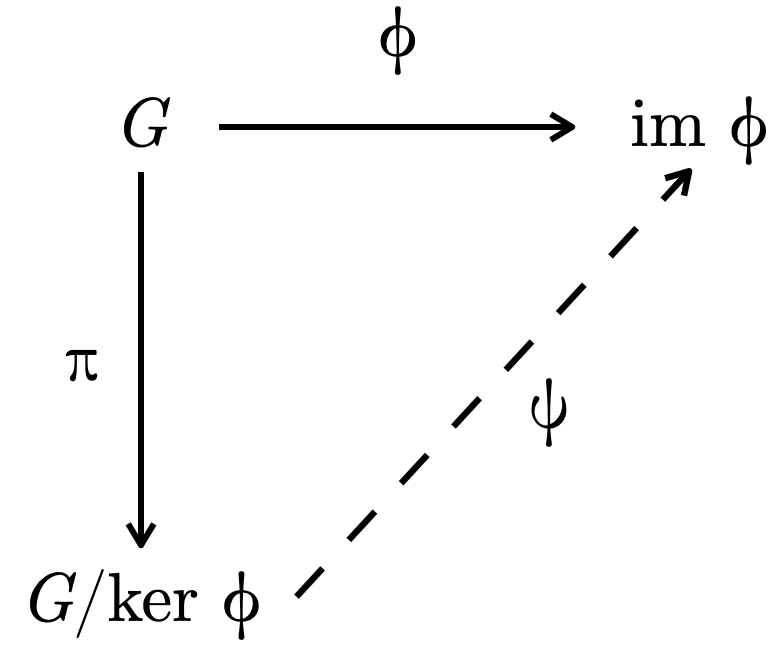
\includegraphics[width=4.5cm]{images/chapter7/FirstIsomorphismTheoremCommutivityDiagram.png}}
    \caption{Commutivity Diagram For \textbf{Theorem \ref{thrm-first-isomorphism}}}
\end{figure}

In the diagram, $\phi$ sends elements from $G$ to $\im\phi$ and $\pi$ sends elements from $G$ to $G/\ker\phi$. Then the map $\psi$ is a unique map that sends elements from $G/\ker\phi$ to the image of $\phi$.

\begin{proof}
    We know by \textbf{Proposition \ref{prop-image-is-subgroup-of-codomain}} that $\im\phi \leq H$. Let $\psi: G/\ker\phi \to \im\phi$ such that $\psi(x\ker\phi) = \phi(x)$. We are to check that $\psi$ is a well-defined isomorphism.
    \begin{itemize}
        \item \textbf{Well-defined}: Suppose $x\ker\phi = y\ker\phi$.
        \begin{align*}
            &\implies xy^{-1} \in \ker\phi & (\text{Coset Equality, \textbf{Lemma \ref{lemma-coset-equality}}})\\
            &\implies\phi(xy^{-1}) = e_H & (\text{Definition of kernel})\\
            &\implies\phi(x)\left(\phi(y)\right)^{-1} = e_H & (\text{Definition of homomorphism})\\
            &\implies\phi(x) = \phi(y)
        \end{align*}
        Thus,
        \[
            \underbrace{\psi(x\ker\phi) = \phi(x)}_{\text{Definition of } \psi} = \underbrace{\phi(y) = \psi(y\ker\phi)}_{\text{Definition of } \psi}
        \]
        so $\psi$ is well-defined.

        \item \textbf{Homomorphism}: Note that
        \begin{align*}
            \psi((x\ker\phi)(y\ker\phi)) &= \psi((xy)\ker\phi)\\
            &= \phi(xy)\\
            &= \phi(x)\phi(y)\\
            &= \psi(x\ker\phi)\psi(y\ker\phi)
        \end{align*}
        so $\psi$ is a homomorphism.
        \item \textbf{Injective}: By \textbf{Exercise \ref{exercise-trivial-kernel-means-injective}}, we check that $\psi$ is injective by showing that $\ker\psi$ is trivial, i.e. $\ker\psi = \{\ker\phi\}$.

        Suppose $x\ker\phi\in\ker\psi$. Then $\psi(x\ker\phi) = e_H$ by definition of kernel. Hence $\phi(x) = e_H$ by definition of $\psi$. Hence, $x \in \ker\phi$ by definition of kernel. This means that $xe^{-1} \in \ker\phi$. So $x\ker\phi = e\ker\phi = \ker\phi$ by Coset Equality (\textbf{Lemma \ref{lemma-coset-equality}}) meaning that $\ker\psi = \{\ker\phi\}$. Therefore $\psi$ is injective.

        \item \textbf{Surjective}: Suppose $y$ is in the image of $\phi$, meaning there exists a $x$ in $G$ such that $\phi(x) = y$. Note that $\psi(x\ker\phi) = \phi(x) = y$. Thus $\psi$ is surjective.
    \end{itemize}
    Thus $\psi$ is a well-defined isomorphism.

    We now check that $\psi$ satisfies the requirement that $\psi\pi = \phi$. Let $x \in G$. Note that $\pi(x) = x\ker\phi$, and
    \[
        \psi\pi(x) = \psi(x\ker\phi) = \phi(x)
    \]
    for all $x \in G$, so $\psi\pi = \phi$.

    Finally we show that $\psi$ is unique. Suppose $f: G/\ker\phi \to \im\phi$ is an isomorphism satisfying $f\pi=\phi$. Take $x\ker\phi \in G/\ker\phi$. Note that
    \begin{align*}
        f(x\ker\phi) &= f(\pi(x))\\
        &= (f\pi)(x)\\
        &= \phi(x)\\
        &= (\psi\pi)(x)\\
        &= \psi(\pi(x))\\
        &= \psi(x\ker\phi)
    \end{align*}
    for all $x \in G$, meaning that $f = \psi$. Therefore $\psi$ is unique.

    Hence, $\psi$ is a unique isomorphism satisfying $\psi\pi = \phi$.
\end{proof}

\begin{example}
    Let $R = \{x \ | \ x > 0\}$, $G = \{x \in \mathbb{R} \ | \ x \neq 0\}$, and $H = \{1, -1\}$ be groups under multiplication. We show $G / H \cong R$.

    Consider the map $\phi: G \to R$ where $x \mapsto |x|$. We show that $\phi$ is a homomorphism, then find the image of $\phi$, and finally find its kernel.
    \begin{itemize}
        \item \textbf{Homomorphism}: $\phi$ is a homomorphism since $\phi(xy) = |xy| = |x||y| = \phi(x)\phi(y)$.
        \item \textbf{Image}: We find the image of $\phi$.
        \begin{align*}
            \im\phi &= \{\phi(x) \ | \ x \in G\}\\
            &= \{|x| \ | \ x \neq 0\}\\
            &= \{x \ | \ x > 0\} & (\text{by definition of } |x|)\\
            &= R
        \end{align*}
        which actually means that $\phi$ is surjective.
        \item \textbf{Kernel}: We find the kernel of $\phi$.
        \begin{align*}
            \ker\phi &= \{x \in G \ | \ \phi(x) = 1\} & (\text{since } 1 \text{ is identity in } R)\\
            &= \{x \in G \ | \ |x| = 1\}\\
            &= \{1, -1\}\\
            &= H
        \end{align*}
    \end{itemize}
    Therefore, by the Fundamental Homomorphism Theorem (\textbf{Theorem \ref{thrm-first-isomorphism}}), $G/H \cong R$.
\end{example}

\begin{exercise}
    Let $\phi: G \to H$ be a homomorphism between finite groups $G$ and $H$. Prove that
    \[
        |G| = |\im \phi|\times|\ker \phi|.
    \]
\end{exercise}

\section{The Diamond Isomorphism Theorem}
We now look at the next theorem, called the \textbf{Diamond Isomorphism Theorem} or the \textbf{Second Isomorphism Theorem}.
\begin{theorem}[Diamond Isomorphism Theorem]\label{thrm-second-isomorphism}
    Let $G$ be a group and let $H$ and $K$ be subgroups of $G$. Then
    \begin{enumerate}
        \item $H \cap K \leq H$ and $H \cap K \leq K$; and
        \item $H \leq HK$ and $K \leq HK$.
    \end{enumerate}
    Furthermore, if $N \lhd G$, then
    \begin{enumerate}[start=3]
        \item $HN \leq G$;
        \item $H \cap N \lhd H$;
        \item $N \lhd HN$; and
        \item $H / (H\cap N) \cong HN / N$.
    \end{enumerate}
\end{theorem}
We can capture the overall relationships between the subgroups of $G$ using a \textbf{subgroup lattice}.
\begin{figure}[h]
    \centering
    \fbox{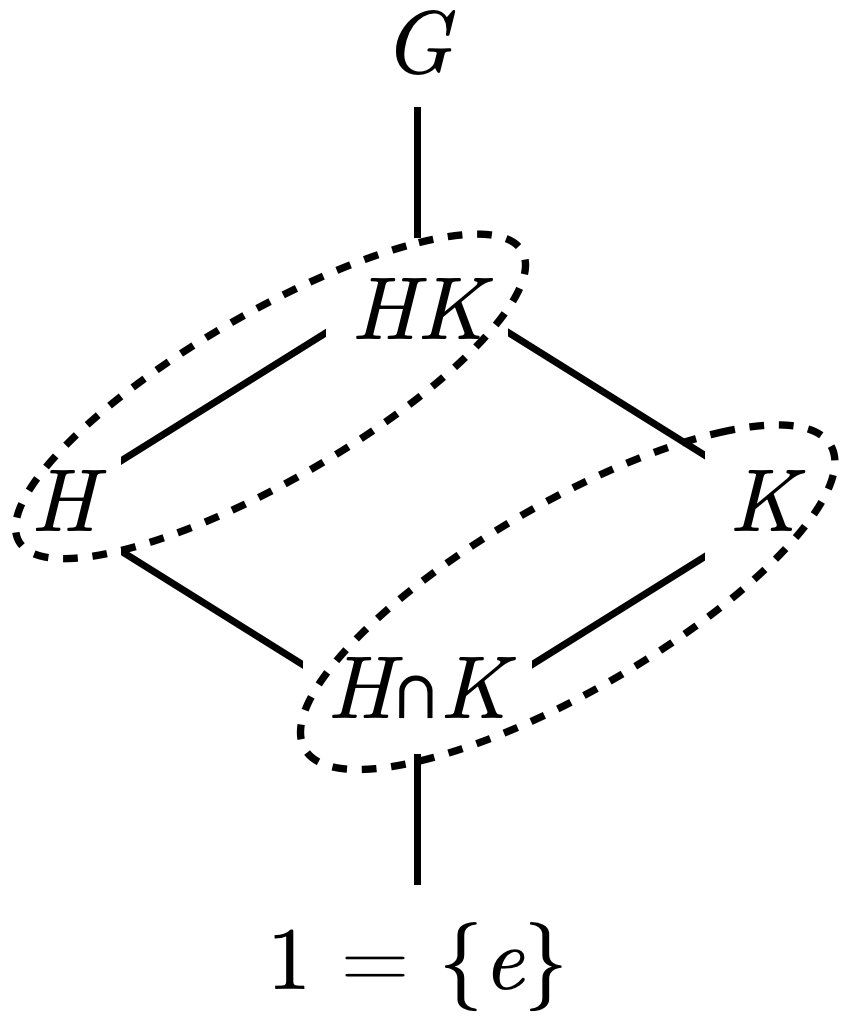
\includegraphics[width=4.5cm]{images/chapter7/SecondIsomorphismTheoremSubgroupDiagram.png}}
    \caption{Subgroup Diagram for \textbf{Theorem \ref{thrm-second-isomorphism}}}
\end{figure}

In the diagram, we only show subgroups that we care about. $G$ has a (direct) subgroup $HK$; $HK$ has subgroups $H$ and $K$; and $H$ and $K$ has a common subgroup $H\cap K$. In the case where $K \lhd G$, the two dotted quotient groups are isomorphic to each other.

\begin{proof}
    We prove each statement in sequence.

    \begin{enumerate}
        \item We only prove the first case (i.e., $H \cap K \leq H$) as the second follows symmetrically.
        
        Clearly $e_G \in H$ and $e_G \in K$ so $e_G \in H \cap K$.
        
        Take $x, y \in H \cap K$. To show that $xy^{-1} \in H \cap K$. Since $x, y \in H \cap K$, thus $x, y \in H$ and $x, y \in K$. Now since $H, K \leq G$, thus $xy^{-1} \in H$ and $xy^{-1} \in K$ by applying the subgroup test on $H$ and $K$ respectively. This thus means that $xy^{-1} \in H \cap K$. By the subgroup test, this means that $H \cap K \leq H$.
        
        \item We only prove the first case ($H \leq HK$) as the second follows symmetrically. Note that $H = \{he_G \ | \ h \in H\} \subseteq \{hk \ | \ h \in H, k \in K\} = HK$, so we consider the subgroup test. Clearly $e_G \in H$ since $H \leq G$. Also since $H \leq G$, for all $x, y \in N$, $xy^{-1} \in G$. Thus, by the subgroup test, $H \leq HN$.
        
        \item We note that, because $N$ is normal, hence $hN = Nh$ for all $h \in H \subseteq G$, meaning that $HN = NH$. Therefore by \textbf{Proposition \ref{prop-subgroup-product-is-subgroup}}, $HN \leq G$.

        \item We know $H \cap N \leq H$ by statement 1, so we only prove normality. Take $x \in H \cap N$, Since $H \leq G$, thus $x \in H \cap N \subseteq H$, meaning for all $g \in H$, $gxg^{-1} \in H$ (where we think of $g$ and $x$ as being in $H$). But since $x \in H \cap N \subseteq N$ and $N \lhd G$, thus $gxg^{-1} \in N$ (where we think of $g \in H$ and $x \in N$). Therefore $H \cap N \lhd H$.

        \item We know $N \leq HN$ by statement 2, so we only prove normality. Take $n \in N$ and $x \in HN$ such that $x = h_xn_x$. Then
        \begin{align*}
            xnx^{-1} &= (h_xn_x)n(h_xn_x)^{-1}\\
            &= (h_xn_x)n(n_x^{-1}h_x^{-1}) & (\text{Shoes and Socks})\\
            &= \underbrace{h_x}_{\text{In }G}\underbrace{n_xnn_x^{-1}}_{\text{In }N}\underbrace{h_x^{-1}}_{\text{In G}}\\
            &\in N
        \end{align*}
        since $N \lhd G$. This proves that $N \lhd HN$.

        \item This is the main result of this theorem.

        We define $\phi: H \to HN/N, h \mapsto hN$. Clearly $\phi$ is a homomorphism as
        \[
            \phi(xy) = (xy)N = (xN)(yN) = \phi(x)\phi(y).
        \]

        We show that $\phi$ is surjective to show that $\im\phi = HN/N$. Suppose $x \in HN$, meaning $x = hn$ where $h \in H$ and $n \in N$. Thus, $xN \in HN/N$. This implies that
        \[
            xN = (hn)N = h(nN) = hN
        \]
        meaning $\phi(h) = hN = xN$. Hence we have found a pre-image of the coset $xN$, meaning $\phi$ is surjective. Hence $\im \phi = HN/N$.

        We now claim that $\ker\phi = H \cap N$. Note that $\ker\phi = \{h \in H \ | \ \phi(h) = eN = N\}$ by definition of kernel. This means that if $h \in \ker\phi$ then $\phi(h) = N$. Hence,
        \[
            \phi(h) = hN = N \implies h \in N
        \]
        by Coset Equality (\textbf{Lemma \ref{lemma-coset-equality}}). Thus, $h \in H$ and $h \in n$, meaning $h \in H \cap N$. Therefore $\ker \phi \subseteq H \cap N$.

        Now suppose $x \in H \cap N$. This means that $x \in N$ necessarily, implying $xN = N$. Thus $\phi(x) = N$ which quickly implies $x \in \ker\phi$. Therefore $H \cap N \subseteq \ker\phi$.

        Since $\ker \phi \subseteq H \cap N$ and  $H \cap N \subseteq \ker\phi$ therefore $\ker\phi = H\cap N$.

        By Fundamental Homomorphism Theorem (\textbf{Theorem \ref{thrm-first-isomorphism}}),
        \[
            H / \ker\phi \cong \im \phi,
        \]
        which means
        \[
            H/(H\cap N) \cong HN/N.
        \]
    \end{enumerate}
    This completes the proof of the Diamond Isomorphism Theorem.
\end{proof}

\begin{corollary}\label{corollary-subgroup-product-is-normal-subgroup-if-subgroups-are-normal}
    Let $G$ be a group. Let $H$ and $K$ be proper normal subgroups of $G$. Then $HK \lhd G$.
\end{corollary}
\begin{proof}
    By the Diamond Isomorphism Theorem (\textbf{Theorem \ref{thrm-second-isomorphism}}), statement 3, we know that $HK \leq G$ since $H \lhd G$. We just need to prove normality. Suppose $hk \in HK$ and take $g \in G$. Then
    \begin{align*}
        g(hk)g^{-1} &= (gh)(kg^{-1})\\
        &= (hg)(g^{-1}k) & (\text{since } H, K \lhd G)\\
        &= h(gg^{-1})k\\
        &= hk \in HK
    \end{align*}
    which means that $HK \lhd G$.
\end{proof}

We look at a few examples for the use of the Diamond Isomorphism Theorem.
\begin{example}
    We say a group $G$ is \textbf{metabelian} if and only if there exists $A \lhd G$ such that $A$ and $G/A$ are both abelian. We will prove the fact that any subgroup of a metabelian group is also metabelian.

    Let $H \leq G$. Then by Diamond Isomorphism Theorem (\textbf{Theorem \ref{thrm-second-isomorphism}}), $H \cap A \lhd H$ (statement 4) and $H/(H \cap A) \cong HA / A$ (statement 6). We just need to prove that $H \cap A$ is abelian and prove that $H/(H \cap A)$ is abelian.
    \begin{itemize}
        \item Consider any two elements from $H \cap A$, say $x$ and $y$. Then $x \in A$ and $y \in A$, meaning $xy = yx$. Hence, elements from $H \cap A$ commute, meaning that $H \cap A$ is abelian.
        \item Consider $HA / A$. Note that $HA \leq G$ since $H \leq G$ and $A \leq G$. Thus, $HA / A \leq G / A$. Note that $G/A$ is abelian by definition of metabelian group. Hence, $H/(H \cap A) \cong HA / A$ is also abelian.
    \end{itemize}
    Therefore, we have found a subgroup of $H$ (in particular $H \cap A$) such that both $H \cap A$ and $H/(H\cap A)$ are both abelian. Hence, $H$ is metabelian.
\end{example}

We look at another application of the Diamond Isomorphism Theorem, which has application in Number Theory.
\begin{example}
    We will prove that $\lcm(m,n)\times\gcd(m,n) = mn$ by considering the Diamond Isomorphism Theorem. For brevity, let $d = \gcd(m,n)$ and $l = \lcm(m,n)$.

    Consider the groups $G = \mathbb{Z}$, $H = m\mathbb{Z}$, and $N = n\mathbb{Z}$ under addition. By Diamond Isomorphism Theorem (\textbf{Theorem \ref{thrm-second-isomorphism}}),
    \[
        m\mathbb{Z}/(m\mathbb{Z} \cap n\mathbb{Z}) \cong (m\mathbb{Z} + n\mathbb{Z})/(n\mathbb{Z}).
    \]

    Now $m\mathbb{Z} \cap n\mathbb{Z}$ is the set of integers that are both a multiple of $m$ and $n$. Hence, $m\mathbb{Z} \cap n\mathbb{Z} = \lcm(m,n)\mathbb{Z} = l\mathbb{Z}$. On the other hand, $m\mathbb{Z} + n\mathbb{Z}$ is the set of all integers of the form $mx+ny$ where $x$ and $y$ are integers. Bezout's identity tells us that this set consists of the multiples of $\gcd(m,n)$, i.e. $m\mathbb{Z} + n\mathbb{Z} = \gcd(m,n)\mathbb{Z} = d\mathbb{Z}$. Hence,
    \[
        m\mathbb{Z}/(l\mathbb{Z}) \cong (d\mathbb{Z})/(n\mathbb{Z}).
    \]

    We claim that
    \[
        m\mathbb{Z} / (l\mathbb{Z}) \cong \mathbb{Z}_{\frac lm} \text{ and } d\mathbb{Z} / (n\mathbb{Z}) \cong \mathbb{Z}_{\frac nd}.
    \]
    This is a specific case of \textbf{Problem \ref{problem-mZ/nZ-isomorphic-to-Zn/m}} which we have left as a problem for later.

    Hence, what we have shown is
    \[
    \mathbb{Z}_{\frac lm} \cong m\mathbb{Z}/(l\mathbb{Z}) \cong d\mathbb{Z}/(n\mathbb{Z}) \cong \mathbb{Z}_{\frac nd}
    \]
    which means that $\mathbb{Z}_{\frac lm} \cong \mathbb{Z}_{\frac nd}$. We can now finally take orders on both sides:
    \[
        \frac{l}{m} = \frac{n}{d},
    \]
    which means that $ld = mn$. Hence, $\lcm(m,n)\times\gcd(m,n) = mn$.
\end{example}

\begin{exercise}\label{exercise-order-of-subgroup-product}
    Let $G$ be a finite group, $H \leq G$, and $N \lhd G$. Prove that
    \[
        |HN| = \frac{|H||N|}{|H \cap N|}.
    \]
\end{exercise}

\newpage

\section{The Third Isomorphism Theorem}
We look at the last important theorem regarding homomorphisms and isomorphisms. This is often called the \textbf{Third Isomorphism Theorem} (e.g. \cite{cohn_1982, hungerford_1980}). It should be noted that there is no consistency with the numbering of these theorems in books (cf. \cite{clark_1984} as ``First Isomorphism Theorem" in \S 68, \cite{humphreys_1996} as Theorem 8.16 ``Second Isomorphism Theorem"), but the name ``Third Isomorphism Theorem'' is the easiest to research. Hence, we use that name here.

\begin{theorem}[Third Isomorphism Theorem]\label{thrm-third-isomorphism}
    Let $G$ be a group. Let $H \lhd G$ and $N \lhd G$. Suppose $N \subseteq H$. Then
    \begin{enumerate}
        \item $N \lhd H$;
        \item $H/N \lhd G/N$; and
        \item $\frac{G/N}{H/N} \cong G/H$
    \end{enumerate}
\end{theorem}
\begin{proof}
    Like with the Diamond Isomorphism Theorem, we will prove the statements in sequence.

    \begin{enumerate}
        \item We first prove that it is a subgroup using the subgroup test before proving normality.

        Since $H, N \leq G$, thus $e_G \in H$ and $e_G \in N$, meaning that $N$ is non-empty. Furthermore, since $N \leq G$, therefore $xy^{-1} \in N$ for all $x, y \in N$. Hence $N \leq H$.

        We now prove normality. Since $H$ and $N$ are normal subgroups of $G$, thus for all $g \in G$,
        \[
            gH = Hg \text{ and } gN = Ng.
        \]
        Now since $N \subseteq H \subseteq G$, thus for all $n$ in $N$, $nH = Hn$ (since $n \in G$). This means that $N \lhd H$.

        \item We first prove that it is a subgroup using the subgroup test, before proving normality.

        Clearly $N = eN \in H/N$. Let $x$ and $y$ be in $H/N$. Then $x=h_xN$ and $y=h_yN$ for some $h_x, h_y \in H$. Note that $y^{-1} = (h_y)^{-1}N$ by group operator on cosets. Hence,
        \begin{align*}
            xy^{-1} &= (h_xN)(h_y^{-1}N)\\
            &= (\underbrace{h_xh_y^{-1}}_{\text{In }H})N\\
            &\in H/N
        \end{align*}
        Hence, by subgroup test, $H/N \leq G/N$.

        Now let $gN \in G/N$ and $hN \in H/N$. We need to show that $(gN)(hN)(gN)^{-1} \in H/N$. Note $(gN)(hN)(gN)^{-1} = (ghg^{-1})N$. Since $H \lhd G$, thus $ghg^{-1} \in H$ which means that $(ghg^{-1})N \in H/N$.

        Therefore $H/N \lhd G/N$.

        \item This is the main result of the theorem.

        Define $\phi: G/N \to G/H, gN \mapsto gH$. We will check that $\phi$ is a well-defined surjective homomorphism and then find its kernel.
        \begin{itemize}
            \item \textbf{Well-defined}: Suppose $gN = g'N$. Then $g(g')^{-1} \in N$ by Coset Equality (\textbf{Lemma \ref{lemma-coset-equality}}). Since $N \subseteq H$ (assumption), thus $g(g')^{-1} \in H$ which implies $gH = g'H$ by \textbf{Lemma \ref{lemma-coset-equality}}. Hence $\phi(gN) = gH = g'H = \phi(g'N)$, i.e. $\phi$ is well-defined.
            \item \textbf{Homomorphism}: Take $gN, g'N \in G/N$. Then
            \begin{align*}
                \phi((gN)(g'N)) &= \phi((gg')N)\\
                &= (gg')H\\
                &= (gH)(g'H)\\
                &= \phi(gN)\phi(g'N)
            \end{align*}
            which means that $\phi$ is a homomorphism.
            
            \item \textbf{Surjective}: Suppose $gH \in G/H$. Then $\phi(gN) = gH$. Thus $gN$ is a pre-image of $gH$, meaning that $\phi$ is surjective.
            
            \item \textbf{Kernel}: Suppose $gN \in \ker\phi = \{gN \ | \ \phi(gN) = eH = H\}$. Thus $\phi(gN) = H \implies gH = H$. Therefore, $ge^{-1} = g \in H$ by \textbf{Lemma \ref{lemma-coset-equality}}. This means that $gN \in H/N$, further meaning that $\ker\phi \subseteq H/N$.

            Suppose now $hN \in H/N$. Since $H \lhd G \implies H\subseteq G$, thus $h \in G$. Therefore $hN \in G/N$ which means $\phi(hN) = hH = H$. Hence $hN \in \ker\phi$ which means $H/N \subseteq \ker\phi$.

            Since $\ker\phi \subseteq H/N$ and $H/N \subseteq \ker\phi$, we must have $\ker\phi = H/N$.
        \end{itemize}

        By Fundamental Homomorphism Theorem (\textbf{Theorem \ref{thrm-first-isomorphism}}), $\frac{G/N}{\ker\phi} \cong \im\phi$ which means
        \[
            \frac{G/N}{H/N} \cong G/H,
        \]
        hence proving statement 3.
    \end{enumerate}
    This proves the theorem.
\end{proof}

\begin{example}
    Take $G = \mathbb{Z}$, $H = m\mathbb{Z}$ and $N = mn\mathbb{Z}$. Note that clearly $H, N \leq G$, and since $G$ is abelian, we must also have $H \lhd G$ and $N \lhd G$. By the Third Isomorphism Theorem (\textbf{Theorem \ref{thrm-third-isomorphism}}),
    \[
        G/H \cong \frac{G/N}{H/N}.
    \]
    Note $G/H = \mathbb{Z}/(m\mathbb{Z}) \cong \mathbb{Z}_m$ by \textbf{Problem \ref{problem-Zn-isomorphic-to-Z-by-nZ}}. Note also
    \[
        \frac{G/N}{H/N} = \frac{\mathbb{Z}/(mn\mathbb{Z})}{m\mathbb{Z}/(mn\mathbb{Z})}
    \]
    and $\mathbb{Z}/(mn\mathbb{Z}) \cong \mathbb{Z}_{mn}$ by \textbf{Problem \ref{problem-Zn-isomorphic-to-Z-by-nZ}}.

    Consider now $\phi: m\mathbb{Z} \to \mathbb{Z}_{mn}, mx \mapsto mx \mod mn$. Clearly $\phi$ is a homomorphism. Note $\im \phi = \langle m \rangle$ and $\ker \phi = mn\mathbb{Z}$. We leave the proof of these claims as an exercise to the reader.

    By the Fundamental Homomorphism Theorem (\textbf{Theorem \ref{thrm-first-isomorphism}}),
    \[
        m\mathbb{Z} / (mn\mathbb{Z}) \cong \langle m \rangle.
    \]
    Thus,
    \[
        \mathbb{Z}_m \cong G/H \cong \frac{G/N}{H/N} \cong \mathbb{Z}_{mn}/\langle m \rangle
    \]
    which means $\mathbb{Z}_m \cong \mathbb{Z}_{mn} / \langle m \rangle$.

    In other words, if $d$ divides $n$, then
    \[
        \mathbb{Z}_n / \langle d \rangle \cong \mathbb{Z}_d.
    \]
\end{example}

From this example we can come up with a more general proposition.
\begin{proposition}\label{prop-Zn-mod-cyclic-subgroup-of-m}
    $\mathbb{Z}_n / \langle m \rangle \cong \mathbb{Z}_{\gcd(m,n)}$
\end{proposition}
\begin{proof}
    We want to show that $\langle m \rangle = \langle \gcd(m,n) \rangle$. For brevity let $\gcd(m,n) = d$.

    \begin{itemize}
        \item $\boxed{\langle m \rangle \leq \langle d \rangle}$ Since $d\;|\;m$, thus $m = dk$ for some integer $k$. Hence, $\langle m \rangle = \{mx \ | \ x \in \mathbb{Z}\} = \{dkx \ | \ x \in \mathbb{Z}\} \leq \langle d \rangle$. Hence, $\langle m \rangle \leq \langle d \rangle d$.
        \item $\boxed{\langle m \rangle \geq \langle d \rangle}$ By the Extended Euclidean Algorithm we may write $d = \alpha m + \beta n$ for some integers $\alpha$ and $\beta$. In $\mathbb{Z}_n$, $d = \alpha m$ which quickly implies that $\langle d \rangle = \langle \alpha m \rangle \leq \langle m \rangle$.
    \end{itemize}
    Therefore $\langle d \rangle = \langle m \rangle$.

    By previous example, the claim is proven.
\end{proof}

\begin{exercise}
    Suppose $x$ and $y$ are positive integers such that $x\;|\;y$. Let $H = x\mathbb{Z}$ and $N = y\mathbb{Z}$ be groups under addition.
    \begin{enumerate}[label=(\roman*)]
        \item Explain why $N \subseteq H$.
        \item Find a group $G$ such that $H \lhd G$ and $N \lhd G$.
        \item Hence find the order of $H/N$.
    \end{enumerate}
\end{exercise}

\newpage

\section{Problems}
\begin{problem}
    Let $G$ be a group. Prove that $G/G \cong \{e\}$.
\end{problem}

\begin{problem}
    Let $G = \mathbb{R}^2$ be a group under component-wise addition,
    \[
        H = \left\{(r\sqrt2, r\sqrt3)\; \vline\;r\in\mathbb{R}\right\}
    \]
    be a group under component-wise addition, and $R = \mathbb{R}$ be a group under addition. Prove that $G/H \cong R$.
\end{problem}

\begin{problem}
    Let $G = \mathbb{Z}^2$ under component-wise addition, $H = \mathbb{Z} \times \mathbb{Z}_5$ under $(+, \oplus_5)$, and $K = \langle(5, 5)\rangle \lhd G$.
    \begin{enumerate}[label=(\roman*)]
        \item Prove that $\phi: G \to H, (m,n) \mapsto (m-n, n \mod 5)$ is a group homomorphism.
        \item Prove that $\phi$ is surjective.
        \item Hence prove $G/K \cong H$.
    \end{enumerate}
\end{problem}

\begin{problem}\label{problem-subgroup-product-equal-to-subgroup-if-one-is-subgroup-of-another}
    Let $G$ be a group. Let $H$ and $K$ be subgroups of $G$ such that $K \subseteq H$. Prove that $HK = H$.
\end{problem}

\begin{problem}\label{problem-cartesian-product-of-group-by-group-isomorphic-to-group}
    Let $G$ be an abelian group under the operation $\ast$. Let $I = \{(g, g^{-1}) \ | \ g \in G\}$ be a group under component-wise application of $\ast$.
    \begin{enumerate}[label=(\roman*)]
        \item Show that $I \cong G$.
        \item Hence prove $G^2/G \cong G$ by considering a suitable homomorphism.
    \end{enumerate}
\end{problem}

\begin{problem}\label{problem-mZ/nZ-isomorphic-to-Zn/m}
    Let $G = m\mathbb{Z}$ and $H = n\mathbb{Z}$ be groups under addition, where $m\;|\;n$ and $m \neq n$. Let the map $\phi: G \to \mathbb{Z}_{\frac nm}$ be defined such that
    \[
        \phi(am) = a \mod \frac{n}{m}.
    \]
    Prove that $G/H \cong \mathbb{Z}_{\frac nm}$.
\end{problem}

%=========================================
\chapter{More Types of Groups}
\section{More About Cyclic Groups}
We previously covered several properties of cyclic groups:
\begin{itemize}
    \item Every cyclic group is abelian. (\textbf{Proposition \ref{prop-cyclic-group-is-abelian}})
    \item A finite group $G$ is cyclic if and only if there exists an element $g$ in the group $G$ with the same order as the group. (\textbf{Theorem \ref{thrm-cyclic-group-has-element-with-same-order}})
    \item If $G$ is cyclic and $H \leq G$ then $G/H$ is cyclic. (\textbf{Exercise \ref{exercise-quotient-group-of-cyclic-group-is-cyclic}})
    \item Any subgroup of a cyclic group is also cyclic. (\textbf{Problem \ref{problem-subgroup-of-cyclic-group-is-cyclic}})
    \item $\mathbb{Z} / (n\mathbb{Z}) \cong \mathbb{Z}_n$. (\textbf{Problem \ref{problem-Zn-isomorphic-to-Z-by-nZ}})
    \item $\mathbb{Z}_m \times \mathbb{Z}_n \cong \mathbb{Z}_{mn}$ if and only if $\gcd(m,n) = 1$. (\textbf{Theorem \ref{thrm-Zm-cross-Zn-isomorphic-to-Zmn-condition}})
    \item $\mathbb{Z}_n / \langle m \rangle \cong \mathbb{Z}_{\gcd(m,n)}$. (\textbf{Proposition \ref{prop-Zn-mod-cyclic-subgroup-of-m}})
    \item $m\mathbb{Z} / n\mathbb{Z} \cong \mathbb{Z}_{\frac nm}$. (\textbf{Problem \ref{problem-mZ/nZ-isomorphic-to-Zn/m}})
\end{itemize}

\begin{exercise}\label{exercise-Zmn-mod-Zn-cong-Zn}
    Prove that for any positive integers $m$ and $n$, we have
    \[
        \mathbb{Z}_{mn} / \mathbb{Z}_m \cong \mathbb{Z}_n.
    \]
\end{exercise}

Note that we may denote the finite cyclic group of order $n$ by $\Cn{n}$ instead of $\mathbb{Z}_n$. This may be sometimes used to distinguish (finite) cyclic subgroups of a group from the integers modulo $n$.

\newpage

We prove more facts about cyclic groups here.
\begin{lemma}\label{lemma-order-of-an-element-that-is-equivalent-to-identity}
    Let $\Cn{n}$ have generator $g$. Then $g^k = e$ if and only if $k$ is a multiple of $n$.\newline
    (Equivalently, this means that if $g^k = e$, then $n$ divides $k$, i.e. $n | k$.)
\end{lemma}
\begin{proof}
    We note that the order of $g$ is $n$, since $g$ is a generator of $G$. Thus by \textbf{Problem \ref{problem-element-to-power-of-multiple-of-order-is-identity}} the lemma is proven.
\end{proof}

\begin{exercise}
    The number 12 is equivalent to 0 in the group $\mathbb{Z}_n$ (under addition modulo $n$). What are the possible value(s) of $n$?
\end{exercise}

We are now ready to prove an important theorem on cyclic groups.
\begin{theorem}\label{thrm-order-of-element-in-cyclic-group}
    Let $\Cn{n}$ have generator $g$. Let $x = g^k$ for some integer $k$. Then the order of $x$ is $\frac{n}{\gcd(k,n)}$.
\end{theorem}
\begin{proof}
    For brevity let $m = |x|$ and suppose $k = \lambda \gcd(k, n)$ for some positive integer $\lambda$.

    Let $\mathcal{X} = \langle x \rangle = \{x, x^2, x^3, \dots, x^m\}$. Note that $\mathcal{X}$ is a cyclic group with order $m$ and generator $x$.

    Observe that
    \[
        x^m = \left(g^k\right)^m = g^{km}
    \]
    and since $|x| = m$, this means that $x^m = e$. Hence
    \[
        g^{km} = e.
    \]

    By \textbf{Lemma \ref{lemma-order-of-an-element-that-is-equivalent-to-identity}} on $\Cn{n}$, $n \vert km$. This implies that
    \[
        \frac{n}{\gcd(k,n)} \ \vline \ \frac{km}{\gcd(k,m)} = \lambda m.
    \]
    Note that $\gcd\left(\lambda, \frac{n}{\gcd(k,n)}\right) = \gcd\left(\frac{k}{\gcd(k,n)}, \frac{n}{\gcd(k,n)}\right) = 1$. This means that $\frac{n}{\gcd(k,n)}$ does not divide $\lambda$, meaning $\frac{n}{\gcd(k,n)} \ \vline \ m$.

    Also note that
    \begin{align*}
        x^{\frac{n}{\gcd(k,n)}} &= \left(g^k\right)^{\frac{n}{\gcd(k,n)}}\\
        &= \left(g^n\right)^{\frac{k}{\gcd(k,n)}}\\
        &= \left(g^n\right)^\lambda\\
        &= e^\lambda & (\text{since } |g| = n)\\
        &= e,
    \end{align*}
    implying $x^{\frac{n}{\gcd(k,n)}} = e$. By \textbf{Lemma \ref{lemma-order-of-an-element-that-is-equivalent-to-identity}} on group $\mathcal{X}$, we have $m \ \vline \ \frac{n}{\gcd(k,n)}$.

    Since $\frac{n}{\gcd(k,n)} \ \vline \ m$ and $m \ \vline \ \frac{n}{\gcd(k,n)}$ simultaneously, thus $m = \frac{n}{\gcd(k,n)}$, i.e. $|x| = \frac{n}{\gcd(k,n)}$.
\end{proof}

\begin{exercise}
    In the group $\mathbb{Z}_{210}$, find the order of 10, 42, 75, and 140.
\end{exercise}

\begin{corollary-thrm}
    Let $\Cn{n}$ have generator $g$. Then $g^m$ is also a generator if and only if $\gcd(m, n) = 1$.
\end{corollary-thrm}
\begin{proof}
    We prove the forward direction first. Suppose that $\Cn{n}$ has a generator of $g^m$. On one hand, $|g^m| = n$ since a generator of a group necessarily has to have an order equal to that of the group. On another hand, by \textbf{Theorem \ref{thrm-order-of-element-in-cyclic-group}}, $|g^m| = \frac{n}{\gcd(m, n)}$. Hence, $n = \frac{n}{\gcd(m, n)}$ which quickly implies $\gcd(m, n) = 1$.

    Now we prove the reverse direction. Suppose $\gcd(m,n) = 1$. Then $|g^m| = \frac{n}{\gcd(m,n)} = \frac{n}{1} = n$ by \textbf{Theorem \ref{thrm-order-of-element-in-cyclic-group}}. Hence $g^m$ is a generator of the group $\Cn{n}$ by \textbf{Theorem \ref{thrm-cyclic-group-has-element-with-same-order}}.
\end{proof}

\begin{exercise}
    Find all the generators of the following groups.
    \begin{enumerate}[label=(\alph*)]
        \item $\mathbb{Z}_{10}$
        \item $\mathbb{Z}_{101}$
    \end{enumerate}
\end{exercise}

\section{Quaternion Group}
We look at an interesting group that has use in computer graphics: the \textbf{Quaternion Group}. We present one definition here.
\begin{definition}
    The quaternion group is denoted by $\mathrm{Q}$ where
    \[
            \mathrm{Q} = \{1, -1, i, -i, j, -j, k, -k\}
    \]
    such that
    \begin{itemize}
        \item 1 is the identity;
        \item $(-1)^2 = 1$;
        \item $i^2 = j^2 = k^2 = -1$;
        \item $ij = k$ and $ji = -k$;
        \item $jk = i$ and $kj = -i$; and
        \item $ki = j$ and $ik = -j$.
    \end{itemize}
\end{definition}

Note that the proper subgroups of $\mathrm{Q}$ are
\begin{itemize}
    \item $\langle -1 \rangle = \{\pm1\}$;
    \item $\langle i \rangle = \{\pm1, \pm i\}$;
    \item $\langle j \rangle = \{\pm1, \pm j\}$; and
    \item $\langle k \rangle = \{\pm1, \pm k\}$.
\end{itemize}
The correctness of these proper subgroups are left as an exercise to the reader.

With these subgroups, we can write a presentation for $\mathrm{Q}$.

\begin{proposition}
    $\mathrm{Q} = \langle i, j \rangle$ (with relationships as given above).
\end{proposition}
\begin{proof}
    For brevity let $G = \langle i, j \rangle$. We are to prove $G = \mathrm{Q}$.

    We note that $i^0 = 1$, $i^4 = j^4 = 1$ and $ji = -k = -ij = i^3j$. Hence,
    \begin{align*}
        G &= \{1, i, i^2, i^3, j, ij, i^2j, i^3j\}\\
        &= \{1, i, -1, -i, j, ij, -j, -ij\}\\
        &= \{1, -1, i, -i, j, -j, ij, -ij\} & (\text{reordering})\\
        &= \{1, -1, i, -i, j, -j, k, -k\} & (\text{since } ij = k)\\
        &= \mathrm{Q}.
    \end{align*}
    Thus, $\mathrm{Q} = \langle i, j \rangle$.
\end{proof}

Thus, an alternate definition of $\mathrm{Q}$ is as follows:
\[
    \mathrm{Q} = \langle \alpha, \beta \ | \ \alpha^4 = e, \alpha^2 = \beta^2, \text{ and } \beta\alpha = \alpha^3\beta \rangle.
\]
One sees clearly that in this definition, $\alpha = i$ and $\beta = j$.

\begin{exercise}\label{exercise-normal-subgroups-of-quarternion-group}
    Find all the normal subgroups of the quaternion group $\mathrm{Q}$.\newline
    (\textit{Hint: consider \textbf{Problem \ref{problem-subgroup-of-index-2}}}.)
\end{exercise}

\section{Alternating Group}
The alternating group is a very important group in the field of group theory. However, before we can properly define it, we need to introduce the idea of \textbf{transpositions}.

\subsection{Transpositions}
\begin{definition}
    A \textbf{transposition} is a 2-cycle. That is, a transposition $\tau$ is represented as $(a\quad b)$ in cycle notation.
\end{definition}
For example, (1 5), (4 7), (3 6) etc. are transpositions, while (1 4 5), (3 4 6 5 9), (1 3 4 5) etc. are not. One clearly sees that every transposition is its own inverse.

We look at one lemma which can be said to help `decompose' transpositions. Note that line breaks are to be ignored in the following lemma.
\begin{lemma}\label{lemma-decompose-transposition}
    Let a transposition $\tau = (i\quad i+d)$ where $d$ is a positive integer. Then
    \begin{align*}
        & (i\quad i+1)(i+1\quad i+2)\cdots\\
        &\quad (i+d-2\quad i+d-1)(i+d-1\quad i+d)(i+d-2\quad i+d-1)\cdots\\
        &\quad (i+1\quad i+2)(i\quad i+1) = \tau.
    \end{align*}
\end{lemma}
\begin{proof}
    We induct on $d$.

    When $d = 1$, $\tau = (i\quad i+1)$ so it is true.

    Assume that the given representation of $\tau$ holds for some positive integer $d$. Note this means that it holds for all $i$, including $i+1$. We are to show that it works for $d + 1$.
    \begin{align*}
        (i\quad i+(d+1)) &= (i\quad i+1)(i+1\quad i+d+1)(i\quad i+1)\\
        &= (i\quad i+1)\underbrace{((i+1)\quad (i+d)+1)}_{\text{apply induction hypothesis}}(i\quad i+1)\\
        &= (i\quad i+1)((i+1)\quad(i+1)+1)\cdots\\
        &\quad\quad((i+1)\quad(i+1)+1)(i\quad i+1)\\
        &= (i\quad i+1)(i+1\quad i+2)\cdots(i+1\quad i+2)(i\quad i+1)
    \end{align*}
    which shows that $d+1$ works as well.
\end{proof}
\begin{remark}
    In the above `decomposition' of $\tau$, $2d-1$ compositions were used.
\end{remark}
\begin{example}
    As an example, let's look at the `decomposition' of the transposition (4 9):
    \[
        (4\quad 9) = (4\quad 5)(5\quad 6)(6\quad 7)(7\quad 8)(8\quad 9)(7\quad 8)(6\quad 7)(5\quad 6)(4\quad 5).
    \]
    We leave it as an exercise for the reader to verify this particular case.
\end{example}
\begin{exercise}
    `Decompose' the transposition (2 6).
\end{exercise}
\begin{remark}
    We call transpositions which take the form $\begin{pmatrix}i&i+1\end{pmatrix}$ \textbf{adjacent transpositions}, and we may denote them by $\alpha$.
\end{remark}

\subsection{Links with Permutations}
As mentioned before, transpositions are a 2-cycle permutation. However, transpositions are important as every permutation can be expressed as a product of transpositions.
\begin{lemma}\label{lemma-permutations-as-product-of-transpositions}
    Every permutation can be expressed as a product of transpositions.
\end{lemma}
\begin{proof}[Proof (see {\cite[\S 80 Corollary]{clark_1984}})]
    For the identity $\id$ it can be expressed as $(a\quad b)(a \quad b)$. For any permutation with length $k \geq 2$, say $\sigma = \begin{pmatrix}a_1 & a_2 & a_3 & \cdots & a_k\end{pmatrix}$, write
    \[
        \sigma = \begin{pmatrix}a_1 & a_k\end{pmatrix}\begin{pmatrix}a_1 & a_{k-1}\end{pmatrix}\begin{pmatrix}a_1 & a_{k-2}\end{pmatrix}\cdots\begin{pmatrix}a_1 & a_3\end{pmatrix}\begin{pmatrix}a_1 & a_2\end{pmatrix}
    \]
    and since every permutation is a product of cycles, thus every permutation is a product of transpositions.
\end{proof}

We now look at the idea of \textbf{inversions} inside permutations.
\begin{definition}
    Let $\sigma$ be a permutation. An \textbf{inversion} of $\sigma$ between $i$ and $j$ exists if $i > j$ and $\sigma(i) < \sigma(j)$.
\end{definition}
An inversion between $i$ and $j$ is denoted by either $(i, j)$ or $(\sigma(i), \sigma(j))$.
\begin{example}
    In the permutation $\sigma = \begin{pmatrix}1 & 3 & 2 & 4\end{pmatrix}$, we see that $3 \mapsto 2$ but $2 \mapsto 4$. Thus there is an inversion (3, 2) = (2, 4).
\end{example}

We now define the idea of \textbf{even} permutations and \textbf{odd} permutations.
\begin{definition}
    A permutation $\sigma$ is said to be \textbf{even} if there are an even number of inversions in $\sigma$. If $\sigma$ is not even then it is said to be \textbf{odd}.
\end{definition}

Counting the number of inversions in a permutation may be too hard to do, and so we have an alternative definition for the evenness or oddness of a permutation. This idea is recorded in the following theorem.

\begin{theorem}\label{thrm-parity-of-permutation}
    Let $\sigma$ be a permutation. Then $\sigma$ is even if and only if the number of transpositions that $\sigma$ is `decomposed' into is even.
\end{theorem}
\begin{proof}
    We only need to show that the \textit{parity} of the number of inversions and permutations are equal to prove this.

    By \textbf{Lemma \ref{lemma-permutations-as-product-of-transpositions}}, all permutations can be produced by a sequence of transpositions, say $\sigma = \tau_1\tau_2\tau_3\cdots\tau_k$.

    By \textbf{Lemma \ref{lemma-decompose-transposition}}, every transposition can be written as a product of $2d - 1$ adjacent transpositions. Decomposing each $\tau_1, \tau_2, \dots, \tau_k$ yields
    \[
        \sigma = \alpha_1\alpha_2\cdots\alpha_m
    \]
    where $\alpha_i$ is an adjacent transposition for $1 \leq i \leq m$. Note that the parity of $m$ is the same as that of $k$.

    It is clear that for any permutation $\pi$ and adjacent permutation $\alpha$, $\alpha\pi$ has either one more or one less inversion than $\pi$. Thus the parity of the number of inversions of a permutation is switched when composed with adjacent transpositions.

    One sees clearly that the identity permutation $\id$ is an even permutation. So $\alpha_1$ is odd, $\alpha_1\alpha_2$ is even, $\alpha_1\alpha_2\alpha_3$ is odd, etc., so $\alpha_1\alpha_2\cdots\alpha_m$ has parity of $m$. Therefore the parity of the number of inversions of $\sigma$ is the parity of $k$, proving the theorem.
\end{proof}

\begin{proposition}\label{prop-permutation-and-inverse-have-same-parity}
    Let $\sigma$ be a permutation. If $\sigma$ is even then $\sigma^{-1}$ is also even. Otherwise if $\sigma$ is odd then $\sigma^{-1}$ is also odd.
\end{proposition}
\begin{proof}
    One observes clearly that $\sigma\sigma^{-1} = \id$. Since $\id$ is even, thus $\sigma\sigma^{-1}$ must be composed of an even number of transpositions (by \textbf{Theorem \ref{thrm-parity-of-permutation}}).
    \begin{itemize}
        \item If $\sigma$ is even, then $\sigma$ is `made up of' an even number of transpositions. Hence $\sigma^{-1}$ must also be `made up of' an even number of transpositions in order for $\sigma\sigma^{-1} = \id$ to be `made up of' an even number of transpositions.
        \item If $\sigma$ is odd, then $\sigma$ is `made up of' an odd number of transpositions. Hence $\sigma^{-1}$ must also be `made up of' an odd number of transpositions in order for $\sigma\sigma^{-1} = \id$ to be even.
    \end{itemize}
    Thus, the proposition is proven.
\end{proof}

We look at one final useful construct: the sign of a permutation.
\begin{definition}
    The \textbf{sign of a permutation} is $+1$ if the permutation is even and $-1$ if the permutation is odd.
\end{definition}
If $\sigma$ is the permutation, $N(\sigma)$ denotes the number of inversions in $\sigma$ and $m$ the number of transpositions in the decomposition of $\sigma$, then the sign of $\sigma$ is given by the signum function:
\[
    \sgn(\sigma) = (-1)^{N(\sigma)} = (-1)^m.
\]
\begin{exercise}
    Find the sign of the permutation (1 3 2 5 4).
\end{exercise}

As a final note, one observes that the number of inversions in $\sigma\tau$ is the same as the sum of inversions in $\sigma$ and $\tau$ separately, meaning
\[
    N(\sigma\tau) = N(\sigma) + N(\tau)
\]
which hence means that the sign of a permutation $\sigma\tau$ is
\begin{align*}
    \sgn(\sigma\tau) &= (-1)^{N(\sigma\tau)}\\
    &= (-1)^{N(\sigma) + N(\tau)}\\
    &= (-1)^{N(\sigma)}(-1)^{N(\tau)}\\
    &= \sgn(\sigma)\sgn(\tau),
\end{align*}
meaning that $\sgn$ is a \textit{multiplicative map}. One can then quickly verify \textbf{Proposition \ref{prop-permutation-and-inverse-have-same-parity}} by noting
\[
    1 = \sgn(\id) = \sgn(\sigma\sigma^{-1}) = \sgn(\sigma)\sgn(\sigma^{-1})
\]
which means $\sgn(\sigma)$ and $\sgn(\sigma^{-1})$ have the same parity.

\newpage

\subsection{The Alternating Group}
We are now ready to look at the alternating group.
\begin{definition}
    The \textbf{alternating group of degree $n$} (where $n \geq 2$), denoted by $\An{n}$, is given by
    \[
        \An{n} = \left\{\sigma \in \Sn{n} \ | \ \sigma \text{ is even}\right\}
    \]
\end{definition}

\begin{proposition}\label{prop-An-normal-subgroup-of-Sn}
    $\An{n} \lhd \Sn{n}$ where $n > 1$.
\end{proposition}
\begin{proof}
    Clearly from definition $\An{n} \subseteq \Sn{n}$ so we consider the subgroup test. Note that the identity function $\id \in \An{n}$ since $\id \in \Sn{n}$ and the identity is even.

    Suppose now that $\mu$ and $\sigma$ are in $\An{n}$. We are to show that $\mu\sigma^{-1} \in \An{n}$. By \textbf{Lemma \ref{lemma-permutations-as-product-of-transpositions}}, we may write
    \[
        \mu = \tau_1\tau_2\cdots\tau_{2k} \text{ and } \sigma = \tau_1'\tau_2'\cdots\tau_{2m}'.
    \]
    We note that any transposition is its own inverse, i.e. $\tau = \tau^{-1}$. Hence by Shoes and Socks, $\sigma^{-1} = \tau_{2m}'\tau_{2m-1}'\cdots\tau_2'\tau_1'$. Therefore,
    \[
        \mu\sigma^{-1} = \underbrace{\tau_1\cdots\tau_{2k}\tau_{2m}'\cdots\tau_1'}_{2(k+m) \text{ transpositions}}
    \]
    is an even permutation, meaning $\mu\sigma^{-1} \in \An{n}$. By subgroup test, $\An{n} \leq \Sn{n}$.
    
    Now take $\sigma \in \Sn{n}$ and $\mu \in \An{n}$. Note that
    \[
        \sgn(\sigma\mu\sigma^{-1}) = \sgn(\sigma)\sgn(\mu)\sgn(\sigma^{-1}).
    \]
    As above, we note $\sgn(\sigma)\sgn(\sigma^{-1}) = 1$ and $\sgn(\mu) = 1$ since $\mu$ is even. Hence $\sgn(\sigma\mu\sigma^{-1}) = 1$ which means that $\sigma\mu\sigma^{-1}$ is an even permutation. Therefore $\sigma\mu\sigma^{-1} \in \An{n}$, meaning that $\An{n} \lhd \Sn{n}$.
\end{proof}

\newpage

\begin{proposition}\label{prop-order-of-An}
    The order of $\An{n}$ is $\frac{n!}{2}$ for $n > 1$.
\end{proposition}
\begin{proof}
    For brevity, let
    \[
        \mathrm{O}_n = \left\{\sigma \in \Sn{n} \ | \ \sigma \text{ is odd}\right\} = \Sn{n} \setminus \An{n}.
    \]
    Clearly $A_n \cup \mathrm{O}_n = \Sn{n}$ and $A_n \cap \mathrm{O}_n = \emptyset$.

    Define a map $f: \An{n} \to \mathrm{O}_n$ such that $\sigma \mapsto \begin{pmatrix}1 & 2\end{pmatrix}\sigma$. We will show that this is a bijective map.
    \begin{itemize}
        \item \textbf{Injective}: Let $\mu$ and $\sigma$ be in $\An{n}$ such that $f(\mu) = f(\sigma)$. This means that $\begin{pmatrix}1 & 2\end{pmatrix}\mu = \begin{pmatrix}1 & 2\end{pmatrix}\sigma$. Now by left-applying $\begin{pmatrix}1 & 2\end{pmatrix}$ on both sides yields $\mu = \sigma$.
        \item \textbf{Surjective}: Take $\mu \in \mathrm{O}_n$, say $\mu = \tau_1\tau_2\cdots\tau_{2k-1}$. Clearly,
        \[
            \mu = \underbrace{\begin{pmatrix}1 & 2\end{pmatrix}\begin{pmatrix}1 & 2\end{pmatrix}}_{\id}\tau_1\tau_2\cdots\tau_{2k-1}.
        \]
        Consider $\sigma = \begin{pmatrix}1 & 2\end{pmatrix}\tau_1\tau_2\cdots\tau_{2k-1}$, which is an even bijective function and thus is in $\An{n}$. Observe that
        \begin{align*}
            f(\sigma) &= \begin{pmatrix}1 & 2\end{pmatrix}\sigma\\
            &= \begin{pmatrix}1 & 2\end{pmatrix}\left(\begin{pmatrix}1 & 2\end{pmatrix}\tau_1\tau_2\cdots\tau_{2k-1}\right)\\
            &= \tau_1\tau_2\cdots\tau_{2k-1}\\
            &= \mu
        \end{align*}
        which means that $\mu \in \mathrm{O}_n$ has a pre-image $\sigma$ in $\An{n}$.
    \end{itemize}
    This proves that $f$ is bijective. Therefore $|\An{n}| = |\mathrm{O}_n|$. Since $A_n \cup \mathrm{O}_n = \Sn{n}$ and $A_n \cap \mathrm{O}_n = \emptyset$, thus $|\Sn{n}| = |\An{n}| + |\mathrm{O}_n| = 2|\An{n}|$. Now because $|\Sn{n}| = n!$ by \textbf{Exercise \ref{exercise-order-of-Sn}}, therefore $|\An{n}| = \frac{n!}2$.
\end{proof}

\begin{exercise}
    List all elements of $\An{3}$.
\end{exercise}

\newpage

\section{Group of Units Modulo \texorpdfstring{$n$}{n}}
We look at a useful group in number theory: the \textbf{group of units modulo $n$}.

\begin{definition}
    For a positive integer $n \geq 2$, the \textbf{group of units modulo $n$}, denoted by $\Un{n}$, is the set
    \[
        \Un{n} = \{m \in \mathbb{Z} \ | \ 1 \leq m < n \text{ and } \gcd(m, n) = 1\}
    \]
    together with the operation $\otimes_n$ (multiplication modulo $n$).
\end{definition}
\begin{proposition}
    $\Un{n}$ is an abelian group.
\end{proposition}
\begin{proof}
    We note that multiplication modulo $n$ is commutative. So, we only need to prove that $\Un{n}$ satisfies the four group axioms to show that $\Un{n}$ is an abelian group.
    \begin{enumerate}
        \item \textbf{Closure}: Let $x, y \in \Un{n}$. Then $\gcd(x, n) = \gcd(y, n) = 1$. Hence $\gcd(xy, n) = 1$ which means that $\gcd(x\otimes_ny,n)=1$. Thus $x\otimes_ny \in \Un{n}$.
        \item \textbf{Associativity}: Since multiplication is associative, this is true.
        \item \textbf{Identity}: Note that 1 is the identity in $\Un{n}$ since $1 \otimes_n x = x$.
        \item \textbf{Inverse}: Let $x$ be in $\Un{n}$, meaning $\gcd(x, n) = 1$. Thus there exists integers $p$ and $q$ such that $px + qn = 1$. Note that $qn$ is a multiple of $n$, so $px \equiv 1 \pmod{n}$, which implies that $p \otimes_n x = 1$. Thus $p$ is the left-inverse of $x$. Since multiplication is commutative, $p$ is also the right-inverse of $x$. Hence $p$ is the inverse of $x$.
    \end{enumerate}
    This thus shows that $\Un{n}$ is an abelian group under $\otimes_n$.
\end{proof}

\begin{exercise}
    List the elements of $\Un{10}$.
\end{exercise}

There is, of course, another representation of $\Un{n}$, but we leave it to later in this section.

A useful number theory function that will occur frequently in this section is \textbf{Euler's totient function}.
\begin{definition}
    The \textbf{Euler totient function} $\totient$ gives the number of numbers which are smaller than and coprime to a number $x$. That is,
    \[
        \totient(x) = |\{n \in \mathbb{Z} \ | \ 1 \leq n < x \text{ and } \gcd(n, x) = 1\}|.
    \]
\end{definition}
In particular, if $x = p_1^{n_1}p_2^{n_2}\cdots p_k^{n_k}$ where $p_1, p_2,\dots,p_k$ are distinct primes and $n_1,n_2,\dots,n_k$ are positive integers, then
\[
    \totient(x) = x \left(1 - \frac1{p_1}\right)\left(1 - \frac1{p_2}\right)\cdots\left(1 - \frac1{p_k}\right).
\]
Note by definition of $\Un{n}$, $|\Un{n}| = \phi(n)$.

\begin{exercise}\label{exercise-order-of-a-divides-phi-a}
    Let $a$ be in $\Un{n}$. Prove that $|a|$ divides $\totient(n)$.
\end{exercise}

We look at the specific case where $|a| = \totient(n)$.
\begin{definition}
    If $\gcd(a, n) = 1$ we say that $a$ is a \textbf{primitive root modulo $n$} if $|a| = \totient(n)$ in $\Un{n}$.
\end{definition}
We state the following fact without proof:
\begin{quote}
    There is a primitive root modulo $n$ if and only if $n$ is 1, 2, 4, $p^k$, or $2p^k$ where $p$ is an odd prime.
\end{quote}

\begin{proposition}\label{prop-Un-cyclic-only-if-exists-primitive-root}
    $\Un{n}$ is cyclic if and only if there is a primitive root modulo $n$.
\end{proposition}
\begin{proof}
    We first prove the forward direction. Let $\Un{n}$ be cyclic. Then there exists an element $r \in \Un{n}$ such that $|r| = |\Un{n}| = \totient(n)$. By definition of a primitive root, this means that $r$ is a primitive root modulo $n$.

    We prove the reverse direction. Let $r \in \Un{n}$ be a primitive root modulo $n$. Then $\langle r \rangle \cong \mathbb{Z}_{\totient(n)}$. Note that since $|\langle r \rangle| = \phi(n) = |\Un{n}|$, therefore $r$ is a generator of $\Un{n}$, proving that $\Un{n}$ is cyclic.
\end{proof}
\begin{remark}
    In fact, what \textbf{Proposition \ref{prop-Un-cyclic-only-if-exists-primitive-root}} shows is that $\Un{n} \cong \mathbb{Z}_{\totient(n)}$ if there exists a primitive root modulo $n$.
\end{remark}

We look at some results about the structure of the group of units.
\begin{proposition}\label{prop-group-of-units-multiplicative-isomorphism}
    If $\gcd(m, n) = 1$ then $\Un{m} \times \Un{n} \cong \Un{mn}$.
\end{proposition}

\begin{proof}
    Let $(x, y) \in \Un{m} \times \Un{n}$. Set $a = n^{-1}$ in $\Un{m}$ and $b = m^{-1}$ in $\Un{n}$.

    Define $\sigma: \Un{m} \times \Un{n} \to \Un{mn}$, where $(x, y) \mapsto xmb + yna$. We show that $\sigma$ is an isomorphism:
    \begin{itemize}
        \item \textbf{Homomorphism}: Consider two pairs $(x_1, y_1)$ and $(x_2, y_2)$.
            \begin{align*}
                \sigma((x_1, y_1)(x_2, y_2)) &= \sigma((x_1x_2, y_1y_2))\\
                &= \underbrace{x_1x_2mb + y_1y_2na}_{\text{In } \Un{mn}}\\
                &= x_1x_2mb + y_1y_2na + \underbrace{x_1y_2mnab + x_2y_1mnab}_{\equiv 0 \pmod{mn}}\\
                &= (x_1mb + y_1na) \otimes_{mn} (x_2mb + y_2na)\\
                &= \sigma((x_1,y_1))\sigma((x_2,y_2))
            \end{align*}
            which shows that $\sigma$ is a homomorphism.
        \item \textbf{Injective}: Suppose $(x_1, y_1)$ and $(x_2, y_2)$ are pairs in $\Un{m}\times\Un{n}$ such that $\sigma((x_1, y_1)) = \sigma((x_2, y_2))$. Then
        \[
            x_1mb + y_1na = x_2mb + y_2na
        \]
        Reducing both sides by modulo $m$ yields $0 + y_1na \equiv 0 + y_2na$. Note that $a = n^{-1}$ in $\Un{m}$, which quickly means $y_1 = y_2$ since $1 \leq y_1, y_2 < n$. Similar argument by reducing both sides by modulo $n$ yields $x_1 = x_2$. This means that $\phi$ is injective.
        \item \textbf{Surjective}: Note that a property of Euler's totient function is that $\totient(mn) = \totient(m)\totient(n)$. Thus
        \[
            |\Un{mn}| = \totient(mn) = \totient(m)\totient(n) = |\Un{m}||\Un{n}| = |\Un{m} \times \Un{n}|.
        \]
        Since $\sigma$ is injective, and since $\Un{mn}$ is equinumerous with $\Un{m} \times \Un{n}$, $\sigma$ has to be surjective.
    \end{itemize}
    This proves that $\sigma$ is an isomorphism between $\Un{m} \times \Un{n}$ and $\Un{mn}$, i.e. $\Un{m} \times \Un{n} \cong \Un{mn}$.
\end{proof}

\begin{proposition}\label{prop-Un-2^m}
    For $m \geq 3$, $\Un{2^m} \cong \mathbb{Z}_{2^{m-2}} \times \mathbb{Z}_2$.
\end{proposition}
\begin{proof}
    We first claim that $|5| = 2^{m-2}$ in $\Un{2^m}$. We induct on $m$ using two-step induction.

    We first consider the case $m = 3$; we are to show that $|5| = 2$ in $\Un{2^3} = \Un{8}$. Since $5^2 = 25 = 24 + 1 \equiv 1 \pmod{8}$, thus $|5| = 2$ in $\Un{8}$, meaning the case where $m = 3$ is true.

    We next consider the case where $m = 4$; we are to show that $|5| = 4$ in $\Un{2^4} = \Un{16}$. Note that $5^1 = 5$, $5^2 = 25 \equiv 9 \pmod{16}$, $5^3 = 125 \equiv 13 \pmod{16}$, and $5^4 = 625 \equiv 1 \pmod{16}$, so $|5| = 4$ in $\Un{16}$, meaning the case where $m = 4$ is true.

    Now assume that the cases where $m = k$ and $m = k+1$ are true for $k \geq 3$, meaning $|5| = 2^{k-2}$ for $\Un{2^k}$ and $|5| = 2^{k-1}$ for $\Un{2^{k+1}}$. To prove that the case where $m=k+2$ is true, that is $|5| = 2^k$ for $\Un{2^{k+2}}$.

    By induction hypothesis, since $|5| = 2^{k-1}$ for $\Un{2^{k+1}}$,
    \[
        5^{2^{k-1}} \equiv 1 \pmod{2^{k+1}} \text{ and } 5^{2^{k-2}} \not\equiv 1 \pmod{2^{k+1}}
    \]
    since $2^{k-1} > 2^{k-2}$ and by definition of the order of the element 5. But since $|5| = 2^{k-2}$ for $\Un{2^k}$, thus
    \[
        5^{2^{k-2}} \equiv 1 \pmod{2^k}.
    \]
    This implies that $5^{2^{k-2}} \equiv 1 + 2^k \pmod{2^{k+1}}$. Now if we reduce modulo $2^{k+2}$ instead,
    \[
            5^{2^{k-2}} \equiv 1 + 2^k + b2^{k+1} \pmod{2^{k+2}}
    \]
    where $b \in \{0, 1\}$. Squaring both sides,
    \begin{align*}
        5^{2^{k-1}} &\equiv \left(1+2^k+b2^{k+1}\right)^2\\
        &\equiv 1 + 2\left(2^k + b2^{k+1}\right) + \left(2^k + b2^{k+1}\right)^2\\
        &\equiv 1 + 2^{k+1} + 2b(2^{k+1}) + 2^{2k}(1+4b+4b^2)\\
        &\equiv 1 + 2^{k+1} + 2^{k+2}b + 2^{k+2}\left(2^{k-2}(1+4b+4b^2)\right) & (\text{since } k\leq 3)\\
        &\equiv 1+2^{k+1} \pmod{2^{k+2}}\\
        &\not\equiv 1 \pmod{2^{k+2}}
    \end{align*}
    which means that, in summary, $5^{2^{k-1}} \not\equiv 1 \pmod{2^{k+2}}$.

    Now, by \textbf{Exercise \ref{exercise-order-of-a-divides-phi-a}}, $|5|$ divides $\totient(2^{k+2}) = 2^{k+1}$ in $\Un{2^{k+2}}$, meaning that $2^{k+1} = a|5|$ for some integer $a$, i.e. $|5| = \frac1a2^{k+1}$.

    Note that $|5| < 2^{k-1}$ for $\Un{2^{k+2}}$ since $|5| = 2^{k-1}$ for $\Un{2^{k+1}}$. Thus, $|5| \geq 2^{k-1}$.

    But since $5^{2^{k-1}} \not\equiv 1 \pmod{2^{k+2}}$, thus $|5| > 2^{k-1}$. Now because $|5| = \frac1a2^{k+1}$ and $|5| > 2^{k-1}$, thus $|5| = 2^k$ (with $a = 2$) or $|5| = 2^{k+1}$ (with $a = 1$).

    Suppose $|5| = 2^{k+1}$. Then $|5| = 2^{k+1} = |\Un{2^{k+2}}|$, meaning that $\Un{2^{k+2}}$ is cyclic. By \textbf{Proposition \ref{prop-Un-cyclic-only-if-exists-primitive-root}} there must be a primitive root modulo $2^{k+2}$ in this case. However, by the ``fact'' about primitive roots, there is \textbf{not} a primitive root modulo $2^{k+2}$. Thus, $|5| \neq 2^{k+1}$ in $\Un{2^{k+2}}$, meaning that $|5| = 2^k$ in $\Un{2^{k+2}}$. This completes the proof of the claim that $|5| = 2^{m-2}$ in $\Un{2^m}$.

    We can finally prove the main result. Let $H = \langle 5 \rangle$ and let $K = \langle -5^{2^{m-3}} \rangle$. Note that:
    \begin{itemize}
        \item $|\mathbb{Z}_{2^{m-2}}| = 2^{m-2} = |\langle 5 \rangle|$ so $\mathbb{Z}_{2^{m-2}} \cong \langle 5 \rangle \leq \Un{2^m}.$
        \item $|-5^{2^{m-1}}| = 2$ since $\left(-5^{2^{m-3}}\right) \times \left(-5^{2^{m-3}}\right) = 5^{2^{m-2}}$ and $|5| = 2^{m-2}$ in $\Un{2^m}$. Thus $\mathbb{Z}_2 \cong \langle -5^{2^{m-3}} \rangle$.
    \end{itemize}
     We see that $\Un{2^m} = HK$ since $\Un{2^m} = HK$, $H \cap K = \{1\}$ (the identity), and $HK = KH$. By \textbf{Theorem \ref{thrm-direct-product-equivilance}}, $HK \equiv H \times K$ so $\Un{2^m} \equiv H \times K$. But $H \cong \mathbb{Z}_{2^{m-2}}$ and $K \cong \mathbb{Z}_2$. Thus, $\Un{2^m} \cong \mathbb{Z}_{2^{m-2}} \times \mathbb{Z}_2$ for $m \geq 3$.
\end{proof}

\begin{corollary}
    Let $p_1, p_2, \dots, p_k$ be distinct odd primes. Then if $m \geq 3$,
    \[
        \Un{2^mp_1^{n_1}p_2^{n_2}\cdots p_k^{n_k}} \cong \mathbb{Z}_2\times\mathbb{Z}_{2^{m-2}}\times\mathbb{Z}_{p_1^{n_1} - p_1^{n_1-1}}\times\cdots\times\mathbb{Z}_{p_k^{n_k} - p_k^{n_k-1}}.
    \]
\end{corollary}

\begin{proof}
    We use the previously proved propositions to establish this result. For brevity let $G = \Un{2^mp_1^{n_1}p_2^{n_2}\cdots p_k^{n_k}}$.
    \begin{align*}
        G &\cong \Un{2^m} \times \Un{p_1^{n_1}} \times\cdots\times \Un{p_k^{n_k}} & \text{(\textbf{Prop. \ref{prop-group-of-units-multiplicative-isomorphism}})}\\
        &\cong (\mathbb{Z}_2 \times \mathbb{Z}_{2^{m-2}}) \times \Un{p_1^{n_1}} \times\cdots\times \Un{p_k^{n_k}} & \text{(\textbf{Prop. \ref{prop-Un-2^m}})}\\
        &\cong (\mathbb{Z}_2 \times \mathbb{Z}_{2^{m-2}}) \times \mathbb{Z}_{\totient(p_1^{n_1})} \times\cdots\times \mathbb{Z}_{\totient(p_k^{n_k})} & \text{(\textbf{Prop. \ref{prop-Un-cyclic-only-if-exists-primitive-root}})}\\
        &\cong \mathbb{Z}_2\times\mathbb{Z}_{2^{m-2}}\times\mathbb{Z}_{p_1^{n_1} - p_1^{n_1-1}}\times\cdots\times\mathbb{Z}_{p_k^{n_k} - p_k^{n_k-1}}
    \end{align*}
    proving the result.
\end{proof}
\begin{example}
    Consider $\Un{600}$. Note that $600 = 2^3 \times 3 \times 5^2$. Thus,
    \[
        \Un{600} \cong \mathbb{Z}_2\times\mathbb{Z}_2    \times\mathbb{Z}_2\times\mathbb{Z}_{20},
    \]
    i.e., $\Un{600} \cong (\mathbb{Z}_2)^3 \times \mathbb{Z}_{20}$.
\end{example}

\begin{exercise}
    Find an isomorphism for $\Un{1680}$ in terms of ``$\mathbb{Z}_n$''s.
\end{exercise}

We end this section by looking at an alternate representation of $\Un{n}$. Define the group
\[
    \left(\mathbb{Z}/(n\mathbb{Z})\right)^{\times} = \left\{m + n\mathbb{Z} \ \vert \ m \in \mathbb{Z}, 1 \leq m < n, \text{ and } \gcd(m, n)=1\right\}
\]
under the operation $\ast$ where $(a+n\mathbb{Z})\ast(b+n\mathbb{Z}) = (a\otimes_n b) + n\mathbb{Z}$ for $n \geq 2$. We will show that $\Un{n}$ is isomorphic to this group.
\begin{proof}
    Define the map $\phi: \Un{n} \to \left(\mathbb{Z}/(n\mathbb{Z})\right)^{\times}$ such that $m \mapsto m + n\mathbb{Z}$. We show that $\phi$ is an isomorphism.

    \begin{itemize}
        \item \textbf{Homomorphism}: Let $x, y \in \Un{n}$. Then $\phi$ is a homomorphism since
        \begin{align*}
            \phi(x \otimes_n y) &= (x \otimes_n y) + n\mathbb{Z}\\
            &= (x + n\mathbb{Z}) \ast (y + n\mathbb{Z})\\
            &= \phi(x) \ast \phi(y).
        \end{align*}

        \item \textbf{Injective}: Suppose we have $x, y \in \Un{n}$ such that $\phi(x) = \phi(y)$. Then this means that $x + n\mathbb{Z} = y + n\mathbb{Z}$. Thus
        \[
            \{x + pn \ | \ p \in \mathbb{Z} \} = \ \{y + qn \ | \ q \in \mathbb{Z} \}.
        \]
        Hence we conclude that $x \equiv y \pmod{n}$. But since $1 \leq x, y < n$, therefore we must have $x = y$. Hence, $\phi(x) = \phi(y)$ implies $x = y$, meaning $\phi$ is injective.

        \item \textbf{Surjective}: Let $x + n\mathbb{Z} \in \left(\mathbb{Z}/(n\mathbb{Z})\right)^{\times}$; thus $\gcd(x, n) = 1$. Performing division algorithm on $x$ yields
        \[
            x = qn + r, \text{ where } 0 \leq r < n.
        \]
        Note that
        \begin{align*}
            x + n\mathbb{Z} &= \{x + kn \ | \ k \in \mathbb{Z}\}\\
            &= \{(qn + r) + kn \ | \ k \in \mathbb{Z}\}\\
            &= \{r + n(\underbrace{q+k}_{\text{In } \mathbb{Z}}) \ | \ k \in \mathbb{Z}\}\\
            &= r + n\mathbb{Z}
        \end{align*}
        with $0 \leq r < n$. Note that if $r = 0$, this means that $x = qn$, which means that $\gcd(x, n) = \gcd(qn, n) = n \neq 1$. Thus, $r \neq 0$, meaning $1 \leq r < n$ so $r \in \Un{n}$.

        Observing that $\phi(r) = r + n\mathbb{Z} = x + n\mathbb{Z}$ shows that $x + n\mathbb{Z}$ has a pre-image $r$ in $\Un{n}$, which means that $\phi$ is surjective.
    \end{itemize}

    Thus $\phi$ is an isomorphism, meaning $\Un{n} \cong \left(\mathbb{Z}/(n\mathbb{Z})\right)^{\times}$.
\end{proof}

\section{Groups of Matrices}
\subsection{Introduction to Matrices}
Before we can introduce the groups of matrices, we need to understand what they are, and to learn some operations that can be applied to matrices.

A matrix is a rectangular array numbers, symbols, or expressions, arranged in rows and columns. They are used to represent mathematical objects or properties of objects.

For example,
\[
    \textbf{M} = \begin{pmatrix}
    1 & 2\\
    3 & 4\\
    5 & 6
    \end{pmatrix}
\]
is a matrix. We consider only square matrices, which have the same number of rows as columns. For example,
\[
    \textbf{A} = \begin{pmatrix}
    1 & 2 & 3\\
    4 & 5 & 6\\
    7 & 8 & 9
    \end{pmatrix}, \textbf{B} = \begin{pmatrix}
    -1 & 0 & 1 & 1\\
    1 & 0 & -1 & 1\\
    1 & 1 & 1 & 1\\
    2 & 3 & 3 & 3
    \end{pmatrix}, \textrm{ and } \textbf{C} = \begin{pmatrix}
    x & x^2\\
    x^3 & x^4\\
    \end{pmatrix}
\]
are square matrices. For brevity, for a matrix \textbf{M}, we denote the element in the $i$th row and the $j$th column as $m_{i,j}$ (where $1 \leq i, j \leq n$ with $n$ being the number of rows and columns in \textbf{M}). For example, using the above matrices, $a_{2,2} = 5$, $b_{2,4}=1$, and $c_{1,1} = x$.

We now need to introduce the idea of \textbf{matrix multiplication}. Consider two square matrices \textbf{A} and \textbf{B} with the same number of rows and columns (say, $n$ rows and columns). Let their product, \textbf{AB}, be the matrix \textbf{C}. Then
\[
    c_{i,j} = \sum_{k=1}^n a_{i,k}b_{k,j}
\]
for $1 \leq i, j \leq n$. For example,
\[
    \begin{pmatrix}1 & 2\\3 & 4\end{pmatrix}\begin{pmatrix}5 & 6\\7 & 8\end{pmatrix}
= \begin{pmatrix}1\times5+2\times7 & 1\times6+2\times8\\3\times5+4\times7 & 3\times6+4\times8\end{pmatrix}
= \begin{pmatrix}19 & 22\\43 & 50\end{pmatrix}.
\]
Note that matrix multiplication is \textbf{not} commutative. For example,
\[
\begin{pmatrix}1 & 2\\3 & 4\end{pmatrix}\begin{pmatrix}5 & 6\\7 & 8\end{pmatrix} = \begin{pmatrix}19 & 22\\43 & 50\end{pmatrix} \text{, but } \begin{pmatrix}5 & 6\\7 & 8\end{pmatrix}\begin{pmatrix}1 & 2\\3 & 4\end{pmatrix} = \begin{pmatrix}23 & 34\\31 & 46\end{pmatrix}
\]

\begin{exercise}
    Find the matrix given by the product
    \[
        \begin{pmatrix}1&1&0\\0&1&0\\0&1&1\end{pmatrix}\begin{pmatrix}1&1&1\\1&0&1\\1&1&1\end{pmatrix}.
    \]
\end{exercise}

Matrices can also be `multiplied' by real numbers (known as scalar multiplication). For example,
\[
    1.23\begin{pmatrix}1 & 2\\3 & 4\end{pmatrix} = \begin{pmatrix}1.23 & 2.46\\3.69 & 4.92\end{pmatrix}.
\]

We look at a special kind of square matrix: the \textbf{identity matrix of order $n$}. It is denoted by $\textbf{I}_n$ and it is a matrix with $n$ rows and columns with 1s on the main diagonal and 0s everywhere else. Thus,
\[
    \textbf{I}_2 = \begin{pmatrix}1 & 0\\0 & 1\end{pmatrix},
\textbf{I}_3 = \begin{pmatrix}1 & 0 & 0\\0 & 1 & 0\\0 & 0 & 1\end{pmatrix}, \text{ and }
\textbf{I}_4 = \begin{pmatrix}1 & 0 & 0 & 0\\0 & 1 & 0 & 0\\0 & 0 & 1 & 0\\0 & 0 & 0 & 1\end{pmatrix}.
\]
We note that for any matrix \textbf{M} with $n$ rows and columns,
\[
    \textbf{MI}_n = \textbf{I}_n\textbf{M} = \textbf{M}.
\]

A square matrix may have an \textbf{inverse}. Consider a square matrix \textbf{A} with $n$ rows and columns. Then \textbf{B} is an inverse of \textbf{A} if
\[
    \textbf{AB} = \textbf{BA} = \textbf{I}_n.
\]
For example, consider the matrices
\[
    \textbf{A} = \begin{pmatrix}1&1&0\\ 0&1&0\\ 0&1&1\end{pmatrix} \text{ and } \textbf{B} = \begin{pmatrix}1&-1&0\\ 0&1&0\\ 0&-1&1\end{pmatrix}.
\]
Note that
\[
    \textbf{AB} = \textbf{BA} = \textbf{I}_3
\]
so \textbf{B} is the inverse of \textbf{A} (and \textbf{A} is the inverse of \textbf{B}). We leave the verification of this claim as an exercise. We denote the inverse of a square matrix \textbf{M} by $\textbf{M}^{-1}$. We note that $\textbf{I}_n^{-1} = \textbf{I}_n$ but not prove it here.

One last thing we introduce here is the idea of a \textbf{matrix determinant} (or simply the \textbf{determinant}). The determinant is only well defined for square matrices. The determinant of a square matrix \textbf{A} is denoted by $\det(\textbf{A})$ or just $\det \textbf{A}$. The rule for the determinant changes as we increase the number of rows and columns in the square matrix, so we only look at small cases.
\begin{itemize}
    \item If the square matrix only has one row, then its determinant is the only element in the matrix. Thus, if $\textbf{A} = (a_{1,1})$ then $\det \textbf{A} = a_{1,1}$.
    \item If the square matrix has two rows, such as the matrix $\begin{pmatrix}a & b\\c & d\end{pmatrix}$, then its determinant is $ad-bc$.
    \item If the square matrix has three rows, for example $\begin{pmatrix}a & b & c \\ d & e & f \\ g & h & i\end{pmatrix}$, then its determinant is $aei+bfg+cdh-ceg-bdi-afh$.
\end{itemize}
An important property of the determinant is that it is a \textit{multiplicative map}: for two square matrices \textbf{A} and \textbf{B},
\[
    \det (\textbf{AB}) = \det(\textbf{A}) \times \det(\textbf{B}).
\]
Finally, not all square matrices has an inverse. The necessary and sufficient condition that determines whether a square matrix \textbf{M} has an inverse is whether $\det \textbf{M} \neq 0$. That is,
\[
    \textbf{M}^{-1} \text{ exists if and only if } \det \textbf{M} \neq 0.
\]

\newpage

We leave this subsection with a few properties of the determinant that we state but not prove:
\begin{itemize}
    \item $\det(\textbf{I}_n) = 1$;
    \item $\det(\textbf{M}^{-1}) = \left(\det \textbf{M}\right)^{-1}$; and
    \item $\det(k\textbf{M}) = k^n \det\textbf{M}$ for a matrix \textbf{M} with $n$ rows and columns.
\end{itemize}

\subsection{General Linear Group over the Real Numbers}
With an introduction of matrices out of the way, we can introduce the first of two important matrix groups: the \textbf{General Linear Group of degree $n$} over the real numbers.
\begin{definition}
    The \textbf{General Linear Group of degree $n$} over the real numbers is denoted by $\GL{n}{\mathbb{R}}$ and is the group with set
    \[
        \left\{\textbf{M} \ | \ \text{\textbf{M} is a matrix with } n \text{ rows and columns, and } \det \textbf{M} \neq 0\right\}
    \]
    under matrix multiplication.
\end{definition}
In other words, $\GL{n}{\mathbb{R}}$ is the group of real-valued matrices with $n$ rows and columns that has an inverse. We show that $\GL{n}{\mathbb{R}}$ is in fact a group under matrix multiplication.
\begin{proof}
    We need to prove the four group axioms.
    \begin{enumerate}
        \item \textbf{Closure}: Consider two matrices \textbf{A} and \textbf{B} that are in $\GL{n}{\mathbb{R}}$. Then that necessarily means that $\det \textbf{A} \neq 0$ and $\det \textbf{B} \neq 0$. Since $\det(\textbf{AB}) = (\det \textbf{A})(\det \textbf{B})$, thus $\det(\textbf{AB}) \neq 0$. Therefore $\textbf{AB}$ is also in $\GL{n}{\mathbb{R}}$, meaning that it is closed under matrix multiplication.
        \item \textbf{Associativity}: Consider three matrices \textbf{A}, \textbf{B}, and \textbf{C} in $\GL{n}{\mathbb{R}}$.
        \begin{itemize}
            \item Consider $(\textbf{AB})\textbf{C}$. Let $\textbf{R} = \textbf{AB}$ and $\textbf{S} = (\textbf{AB})\textbf{C}$. Then
            \[
                r_{i,k} = \sum_{l=1}^n a_{i,l}b_{l,k} \text{ and } s_{i,j} = \sum_{k=1}^n r_{i,k}c_{k,j}
            \]
            which means that
            \[
                s_{i,j} = \sum_{k=1}^n \left(\sum_{l=1}^n a_{i,l}b_{l,k}\right)c_{k,j} = \sum_{k=1}^n \sum_{l=1}^n (a_{i,l}b_{l,k})c_{k,j}.
            \]
            \item Now consider $\textbf{A}(\textbf{BC})$. Let $\textbf{R} = \textbf{BC}$ and $\textbf{S} = \textbf{A}(\textbf{BC})$. Then
            \[
                r_{l,j} = \sum_{k=1}^nb_{l,k}c_{k,j} \text{ and } s_{i,j} = \sum_{l=1}^n a_{i,l}r_{l,j}
            \]
            which means that
            \[
                s_{i,j} = \sum_{l=1}^n a_{i,l}\left(\sum_{k=1}^nb_{l,k}c_{k,j}\right) = \sum_{l=1}^n\sum_{k=1}^n a_{i,l}(b_{l,k}c_{k,j}).
            \]
        \end{itemize}
        Now, multiplication is associative. Thus,
        \[
                (a_{i,l}b_{l,k})c_{k,j} = a_{i,l}(b_{l,k}c_{k,j})
        \]
        which means
        \[
            \sum_{k=1}^n \sum_{l=1}^n (a_{i,l}b_{l,k})c_{k,j} = \sum_{l=1}^n\sum_{k=1}^n a_{i,l}(b_{l,k}c_{k,j}),
        \]
        thereby proving that matrix multiplication is associative.
        \item \textbf{Identity}: We note that $\det \textbf{I}_n = 1 \neq 0$, so $\textbf{I}_n$ is in $\GL{n}{\mathbb{R}}$. Since $\textbf{MI}_n = \textbf{I}_n\textbf{M} = \textbf{M}$ for any matrix $\textbf{M}$ in $\GL{n}{\mathbb{R}}$, thus $\textbf{I}_n$ is indeed the identity of $\GL{n}{\mathbb{R}}$.
        \item \textbf{Inverse}: Let \textbf{M} be a matrix in $\GL{n}{\mathbb{R}}$. Consider the matrix $\textbf{M}^{-1}$. By determinant property, we know that $\det \textbf{M}^{-1} = \left(\det \textbf{M}\right)^{-1}$ and since $\det \textbf{M} \neq 0$ thus $\det \textbf{M}^{-1} \neq 0$. Hence $\textbf{M}^{-1}$ is in $\GL{n}{\mathbb{R}}$. Now because $\textbf{MM}^{-1} = \textbf{M}^{-1}\textbf{M} = \textbf{I}_n$, thus $\textbf{M}^{-1}$ is the inverse of \textbf{M} in $\GL{n}{\mathbb{R}}$.

    \end{enumerate}
    Thus $\GL{n}{\mathbb{R}}$ is a group since all four group axioms are satisfied.
\end{proof}

\subsection{Special Linear Group over the Real Numbers}
We look at another group of matrices: the \textbf{Special Linear Group of degree $n$} over the real numbers.
\begin{definition}
    The \textbf{Special Linear Group of degree $n$} over the real numbers is denoted by $\SL{n}{\mathbb{R}}$ and is the group with set
    \[
        \left\{\textbf{M} \ | \ \text{\textbf{M} is a matrix with } n \text{ rows and columns, and } \det \textbf{M} = 1\right\}
    \]
    under matrix multiplication.
\end{definition}
One sees clearly that $\SL{n}{\mathbb{R}}$ is a sub\textit{set} of $\GL{n}{\mathbb{R}}$: the set of $\GL{n}{\mathbb{R}}$ requires non-zero determinant while the set of $\SL{n}{\mathbb{R}}$ requires the determinant to be 1, which obviously satisfies the non-zero determinant requirement. What we want to prove here is that $\SL{n}{\mathbb{R}}$ is a sub\textit{group} of $\GL{n}{\mathbb{R}}$. In fact, $\SL{n}{\mathbb{R}}$ is a \textit{normal} subgroup of $\GL{n}{\mathbb{R}}$.

\begin{proof}
    We consider the subgroup test. Clearly $\textbf{I}_n$ is in $\SL{n}{\mathbb{R}}$ since its determinant is 1. Hence all we have to check the second condition of the subgroup test.

    Let \textbf{A} and \textbf{B} be matrices in the set $\SL{n}{\mathbb{R}}$. This means that
    \[
        \det \textbf{A} = 1 \text{ and } \det \textbf{B} = 1.
    \]
    Note that $\det \textbf{B}^{-1} = (\det \textbf{B})^{-1} = 1^{-1} = 1$. Thus, $\det \textbf{AB}^{-1} = (\det \textbf{A})(\det \textbf{B}^{-1}) = 1 \times 1  = 1$ which means that $\textbf{AB}^{-1}$ is also in $\SL{n}{\mathbb{R}}$. Hence by the subgroup test, $\SL{n}{\mathbb{R}} \leq \GL{n}{\mathbb{R}}$.
    
    Now let $\textbf{M}$ be a matrix in $\GL{n}{\mathbb{R}}$ and $\textbf{N}$ be a matrix in $\SL{n}{\mathbb{R}}$. We are to show that $\textbf{MNM}^{-1}$ is in $\SL{n}{\mathbb{R}}$. Since $\textbf{M} \in \GL{n}{\mathbb{R}}$ thus $\det \textbf{M} \neq 0$, meaning $\det \textbf{M}^{-1} = (\det \textbf{M})^{-1} \neq 0$. Also, $\textbf{N} \in \SL{n}{\mathbb{R}}$ implies $\det \textbf{N} = 1$. Hence,
    \[
        \det \textbf{MNM}^{-1} = (\det \textbf{M})(\det \textbf{N})(\det \textbf{M})^{-1} = \det \textbf{N} = 1
    \]
    which means that $\textbf{MNM}^{-1}$ is in $\SL{n}{\mathbb{R}}$.

    Therefore $\SL{n}{\mathbb{R}} \lhd \GL{n}{\mathbb{R}}$.
\end{proof}

\subsection{A Consequence of the Fundamental Homomorphism Theorem}
We end this section with a corollary of the Fundamental Homomorphism Theorem regarding these groups of matrices. 

For brevity denote $\mathbb{R}^\times$ as the group of non-zero real numbers under multiplication.

\begin{proposition}
    $\GL{n}{\mathbb{R}} / \SL{n}{\mathbb{R}} \cong \mathbb{R}^\times$.
\end{proposition}
\begin{proof}
    Define the map $\phi: \GL{n}{\mathbb{R}} \to \mathbb{R}^\times$ where $\textbf{M} \mapsto \det\textbf{M}$.
	\begin{itemize}
	    \item \textbf{Homomorphism}: Take $\textbf{M}, \textbf{N} \in \GL{n}{\mathbb{R}}$. Then we have
	    \[
	        \phi(\textbf{MN}) = \det \textbf{MN} = \det(\textbf{M})\det(\textbf{N}) = \phi(\textbf{M})\phi(\textbf{N})
	    \]
	    which means that $\phi$ is a homomorphism.

	    \item \textbf{Image}: We prove that $\phi$ is surjective to show that $\im \phi = \mathbb{R}^\times$.

	    Suppose $r \in \mathbb{R}^\times$. Then $r^{\frac1n} \in \mathbb{R}^\times$, and a matrix with $r^{\frac1n}$ on its main diagonal (written as $r^{\frac1n}\textbf{I}_n$ where $\textbf{I}_n$ is the identity matrix with $n$ rows and columns) is in $\GL{n}{\mathbb{R}}$. Note that $\det(r^{\frac1n}\textbf{I}_n) = \left(r^{\frac1n}\right)^n\det(\textbf{I}_n) = r$. Thus there is a pre-image of $r$ inside the codomain $\mathbb{R}^\times$, meaning that $\phi$ is surjective.

	    Hence, $\im \phi = \mathbb{R}^\times$.

	    \item \textbf{Kernel}: Note that 1 is the identity in $\mathbb{R}^\times$. Thus
	    \begin{align*}
	        \ker\phi &= \{\textbf{M} \in \GL{n}{\mathbb{R}} \vert \phi(\textbf{M}) = 1\} \\
	        &= \{\textbf{M} \in \GL{n}{\mathbb{R}} \vert \det(\textbf{M}) = 1\}\\
	        &= \SL{n}{\mathbb{R}}
	    \end{align*}
	    by definition of the group $\SL{n}{\mathbb{R}}$.
	\end{itemize}
	By the Fundamental Homomorphism Theorem (\textbf{Theorem \ref{thrm-first-isomorphism}}), we have
	\[
	    \GL{n}{\mathbb{R}} / \SL{n}{\mathbb{R}} \cong \mathbb{R}^\times,
	\]
	proving the claim.
\end{proof}

\section{Automorphism Groups}
\subsection{Group of Automorphisms of \texorpdfstring{$G$}{G}}
We look at automorphisms, an important type of map that we look in Group Theory.
\begin{definition}
    An \textbf{automorphism} of a group $G$ is an isomorphism from a group $G$ to itself. That is, $\phi: G \to G$ is an automorphism if $\phi$ is an isomorphism.
\end{definition}
Clearly, from this definition, the identity function $\id$ is an automorphism.

We now look at the group of automorphisms of a group $G$.
\begin{definition}
    Let $G$ be a group. The \textbf{group of automorphisms of $G$}, denoted $\Aut{G}$, is given by
    \[
        \Aut{G} = \{\phi: G \to G \ | \ \phi \text{ is an isomorphism}\}
    \]
    under function composition (denoted by $\circ$).
\end{definition}
We prove that $\Aut{G}$ is indeed a group.
\begin{proof}
    We look at the four group axioms.
    \begin{itemize}
        \item \textbf{Closure}: If $f, g \in \Aut{G}$, and $h = fg$, then $h: G \to G$ is a bijection. Furthermore $h$ is a homomorphism since
        \[
            h(xy) = f(g(xy)) = f(g(x)g(y)) = f(g(x))f(g(y)) = h(x)h(y)
        \]
        so $h$ is an isomorphism, meaning $h = fg \in \Aut{G}$.

        \item \textbf{Associativity}: Function composition is associative.

        \item \textbf{Identity}: As mentioned above, the identity isomorphism $\id: G \to G, g \mapsto g$ is in $\Aut{G}$. By definition of $\id$, $f \circ \id = f$ and $\id \circ f = f$, so $\id$ is indeed the identity in $\Aut{G}$.

        \item \textbf{Inverse}: Suppose $f \in \Aut{G}$. Then $f$ is an isomorphism. By \textbf{Theorem \ref{thrm-isomorphism-consequences}}, $f^{-1}: G \to G$ is also an isomorphism, so $f^{-1} \in \Aut{G}$. Recall also that
        \[
            f\circ f^{-1} = \id \text{ and } f^{-1}\circ f = \id
        \]
        so $f^{-1}$ is indeed the identity of $f$.
    \end{itemize}
    Since the four group axioms are satisfied, thus $\Aut{G}$ is a group under function composition.
\end{proof}

\subsection{Group of Inner Automorphisms of \texorpdfstring{$G$}{G}}
We now look at inner automorphisms and its group.
\begin{definition}
    An \textbf{inner automorphism} of a group $G$ is an automorphism $\iota: G \to G$ such that $\iota(x) = gxg^{-1}$ for some fixed $g \in G$.
\end{definition}
\begin{definition}
    Let $G$ be a group. The \textbf{group of inner automorphisms of $G$}, $\Inn{G}$, is given by
    \[
        \Inn{G} = \{\iota_g: G \to G \ | \ \iota_g(x) = gxg^{-1}, g \in G\}
    \]
    under function composition (denoted by $\circ$).
\end{definition}
We prove that $\Inn{G}$ is a subgroup of $\Aut{G}$.
\begin{proof}
    Clearly $\id \in \Inn{G}$ since $\id = \iota_e$ and $\id(x) = \iota_e(x) = exe^{-1} = x$. Hence $\Inn{G}$ is non-empty and, furthermore, $\Inn{G} \subseteq \Aut{G}$.

    Now take $\iota_x, \iota_y \in \Inn{G}$. Note that $\left(\iota_y\right)^{-1} = \iota_{y^{-1}}$ since
    \[
        \left(\iota_y\right)\left(\iota_{y^{-1}}\right)(g) = \left(\iota_y\right)\left(y^{-1}gy\right) = y\left(y^{-1}gy\right)y^{-1} = g
    \]
    which means $\left(\iota_y\right)\left(\iota_{y^{-1}}\right) = \id$. Therefore $\iota_x\left(\iota_y\right)^{-1} = \iota_{xy^{-1}}$ since
    \begin{align*}
        \iota_x\left(\iota_y\right)^{-1}(g) &= \iota_x\iota_{y^{-1}}(g)\\
        &= \iota_x\left(y^{-1}gy\right)\\
        &= xy^{-1}gyx^{-1}\\
        &= xy^{-1}g(xy^{-1})^{-1}\\
        &= \iota_{xy^{-1}}
    \end{align*}
    which means that $\iota_x\left(\iota_y\right)^{-1} = \iota_{xy^{-1}} \in \Inn{G}$.

    Hence, by subgroup test, $\Inn{G} \leq \Aut{G}$.
\end{proof}

\begin{exercise}
    Let $G$ be a group. Prove that $\Inn{G} \lhd \Aut{G}$.
\end{exercise}

\subsection{A Consequence of the Fundamental Homomorphism Theorem}
Before we can state the consequence, we revisit the idea of the center of a group as introduced in \textbf{Example \ref{example-center-of-group}}.
\begin{quote}
    The center of a group $G$ is the normal subgroup
    \[
        \Z{G} = \{z \in G \ | \ gz = zg \text{ for all } g \in G\}.
    \]
    In other words, $\Z{G} = \{z \in G \ | \ z = gzg^{-1} \text{ for all } g \in G\}$.
\end{quote}

\begin{proposition}
    $G/\Z{G} \cong \Inn{G}$.
\end{proposition}
\begin{proof}
    We define $\phi: G \to \Inn{G}, g \mapsto \iota_g$ where $\iota_g(x) = gxg^{-1}$.
    \begin{itemize}
        \item \textbf{Homomorphism}: Let $g, h \in G$. Then for any $x \in G$,
        \begin{align*}
            (\phi(gh))(x) = \iota_{gh}(x) &= (gh)x(gh)^{-1}\\
            &= ghxh^{-1}g^{-1}\\
            &= g(hxh^{-1})g^{-1}\\
            &= g(\iota_h(x))g^{-1}\\
            &=\iota_g(\iota_h(x))\\
            &=(\iota_g\circ\iota_h)(x)\\
            &=(\phi(g)\phi(h))(x)
        \end{align*}
        which means that $\phi$ is a homomorphism.

        \item \textbf{Image}: We show that $\phi$ is surjective to prove that $\im \phi = \Z{G}$. Suppose $\iota_g \in \Inn{G}$. Clearly $\phi(g) = \iota_g$  which means that $\phi$ is surjective.

        \item \textbf{Kernel}: Note that $\ker\phi = \{g \in G \ | \ \phi(g) = \id\}$. So, if $g \in \ker\phi$ then $(\phi(g))(x) = \iota_g(x) = \id(x) = x$ for all $x \in G$. This means that $gxg^{-1} = x \implies gx = xg$ for all $x \in G$, so $g \in \Z{G}$. Hence $\ker\phi = \Z{G}$.
    \end{itemize}
    Therefore, ones sees that by the Fundamental Homomorphism Theorem (\textbf{Theorem \ref{thrm-first-isomorphism}}),
    \[
        G/\ker\phi \cong \im\phi \implies G/\Z{G} \cong \Inn{G}
    \]
    which proves the result.
\end{proof}

\newpage

\section{Problems}
\begin{problem}
    By considering the group $\mathbb{Z}_{10101}$, find the smallest positive integers $a$ and $b$ such that
    \begin{enumerate}[label=(\alph*)]
        \item $1870a$ is a multiple of 10101.
        \item $3774b$ is a multiple of 10101.
    \end{enumerate}
\end{problem}

\begin{problem}
    Find the largest integer $n$ such that $\An{n}$ is abelian, proving your claim. Hence find all integers $k$ such that $\An{k}$ is cyclic.
\end{problem}

\begin{problem}
    Suppose $r$ is an odd primitive root modulo $p^k$, where $p$ is an odd prime and $k \geq 1$. Prove that $r$ is also a primitive root modulo $2p^k$.
\end{problem}

\begin{problem}
    Let $G$ be a finite cyclic group of order $n$ and generator $g$.
    \begin{enumerate}[label=(\roman*)]
        \item Suppose $f: G \to G$ and $h: G \to G$ are homomorphisms. Prove that $f = h$ if and only if $f(g) = h(g)$.
        \item Let $f: G \to G$ be a homomorphism. Explain why $f(g) = g^{m_f}$ where $m_f$ is a integer unique to $f$.
        \item Suppose $f: G \to G$ and $h: G \to G$ are homomorphisms. Prove that $m_{f\circ h} = m_f \otimes_n m_h$, where $\circ$ denotes function composition and $\otimes_n$ denotes multiplication modulo $n$.
        \item Let $f: G \to G$ be a homomorphism. Prove that $f$ is an automorphism if and only if $m_f$ has a multiplicative inverse modulo $n$. That is, there exists $k \in \Un{n}$ such that $m_fk \equiv 1 \pmod n$ if and only if $f$ is an automorphism.\newline
        (\textit{Hint: consider \textbf{Proposition \ref{prop-multiplicative-inverse-exists-iff-coprime}}, where $ab \equiv 1 \pmod m$ if and only if $\gcd(a, m) = 1$.})
        \item Hence, by considering the map $\phi: \Aut{G} \to \Un{n}$ where $f \mapsto m_f$, prove $\Aut{G} \cong \Un{n}$. 
    \end{enumerate}
\end{problem}

%=========================================
\chapter{Group Actions}
\section{Definition and Examples}
A group action is a representation of the elements of a group as symmetries of a set. Many groups have a `natural' group action coming from their construction. For example, the dihedral group of order 6, $D_3$, acts on the vertices of an equilateral triangle because the group is given as a set of symmetries of the equilateral triangle, by definition. A group action of a group on a set is a generalization of this idea, which can be used to derive useful facts about the group and the set it acts on.

\begin{definition}\label{definition-group-action}
    Let $G$ be a group, $e$ be the identity in $G$, and $X$ be a set. A \textbf{group action of $G$ on $X$} is a function $\alpha: G \times X \to X$ satisfying the following conditions.
    \begin{itemize}
        \item \textbf{Identity}: $\alpha(e, x) = x$ for all $x \in X$.
        \item \textbf{Compatibility}: $\alpha(g, \alpha(h, x)) = \alpha(gh, x)$ for all $g, h \in G$ and $x \in X$.
    \end{itemize}
\end{definition}
\begin{remark}
    Some sources will use $f$ (e.g. \cite{brilliant_groupactions}) or $\phi$ (e.g. \cite{rowland_groupaction}) as the group action.
\end{remark}
In this case, the group $G$ is called a \textbf{transformation group} and $X$ is called a \textbf{$G$-set}.

When the action is `obvious', the function $\alpha(g, x)$ is often written as $g \cdot x$ instead. Note that we \textbf{will} write the dot in this book. With this notation, the axioms above become:
\begin{itemize}
    \item $e \cdot x = x$ for all $x \in X$; and
    \item $g \cdot (h \cdot x) = (gh) \cdot x$ for all $g, h \in G$ and $x \in X$.
\end{itemize}

\begin{example}
    Consider $G = \Sn{n}$ and the set $X = \{1, 2, 3, \dots, n\}$. Then $G$ acts on $X$ by the function $\alpha$ such that $\alpha(g, x) = g(x)$. That is, $g \cdot x = g(x)$ in this case. We note that the axioms are satisfied:
    \begin{itemize}
        \item \textbf{Identity}: $\id \cdot x = \id(x) = x$.
        \item \textbf{Compatibility}: $g \cdot (h \cdot x) = g(h(x)) = (g \circ h)(x) = (gh) \cdot x$.
    \end{itemize}
\end{example}

\begin{example}
    Let $G$ be any group and the function $\alpha: G\times G \to G$ be defined such that $\alpha(g, x) = gx$. We show that $\alpha$ is a group action of $G$ on $G$:
    \begin{itemize}
        \item \textbf{Identity}: $e\cdot x = ex = x$.
        \item \textbf{Compatibility}: $g \cdot (h\cdot x) = g \cdot (hx) = ghx = (gh)x = (gh) \cdot x$.
    \end{itemize}
\end{example}

\begin{exercise}\label{exercise-conjugacy-is-group-action}
    Let $G$ be a group and the function $\alpha: G\times G \to G$ be defined such that $\alpha(g, x) = gxg^{-1}$. Show that $\alpha$ is a group action of $G$ on $G$.
\end{exercise}

We note that there is an equivalent definition of a group action from $G$ to $X$.
\begin{definition}\label{definition-group-action-alt}
    Let $G$ be a group and $X$ be a set. Then a group action of $G$ on $X$ is a homomorphism $\phi: G\to \Sym{X}$.
\end{definition}
\begin{theorem}\label{thrm-group-action-definition-equivalence}
    \textbf{Definition \ref{definition-group-action}} and \textbf{Definition \ref{definition-group-action-alt}} are equivalent.
\end{theorem}
\begin{proof}
    We first work forwards, assuming \textbf{Definition \ref{definition-group-action}} holds and proving \textbf{Definition \ref{definition-group-action-alt}} holds as well. Assume $\alpha: G \times X \to X$ is a group action. Define $\psi: G \to \Sym{X}$ by $g \mapsto f_g$ where $f_g: X \to X, x \mapsto \alpha(g, x)$. We show that $f_g$ is in fact a bijection.
    
    \newpage
    
    \begin{itemize}
        \item \textbf{Injective}: Suppose there exists $x, y \in X$ such that $f_g(x) = f_g(y)$. Then,
        \begin{align*}
            x &= \alpha(e, x)\\
            &= \alpha(g^{-1}g, x)\\
            &= \alpha(g^{-1}, \alpha(g, x))\\
            &= \alpha(g^{-1}, f_g(x))\\
            &= \alpha(g^{-1}, f_g(y))\\
            &= \alpha(g^{-1}, \alpha(g, y))\\
            &= \alpha(g^{-1}g, y)\\
            &= \alpha(e, y)\\
            &= y,
        \end{align*}
        which proves that $f_g$ is injective.
        \item \textbf{Surjective}: Suppose $y \in X$. We note that $\alpha(g^{-1}, y) \in X$ by definition of $\alpha$. Hence observe that $f_g(\alpha(g^{-1}, y)) = \alpha(g, \alpha(g^{-1}, y)) = y$, which means that any element $y \in X$ has a pre-image in $X$. This shows that $f_g$ is surjective.
    \end{itemize}
    Hence $f_g$ is a bijection from $X$ to $X$, which means $f_g \in \Sym{X}$. We just need to show that $\psi$ is a homomorphism. Take $x \in X$, and let $g, h \in G$. Then
    \begin{align*}
        (\psi(gh))(x) &= f_{gh}(x)\\
        &= \alpha(gh, x)\\
        &= \alpha(g, \alpha(h, x))\\
        &= \alpha(g, f_h(x))\\
        &= f_g(f_h(x))\\
        &= (f_g \circ f_h)(x)\\
        &= (\psi(g)\psi(h))(x)
    \end{align*}
    for any $x \in X$, which means $\psi(gh) = \psi(g)\psi(h)$. Hence $\phi$ is indeed a homomorphism, satisfying \textbf{Definition \ref{definition-group-action-alt}}.

    We now work in the reverse direction, assuming \textbf{Definition \ref{definition-group-action-alt}} holds and proving \textbf{Definition \ref{definition-group-action}} holds as well. Suppose $\phi: G \to \Sym{X}$ is a group homomorphism. We define $\beta: G \times X \to X$ where $\beta(g, x) = (\phi(g))(x)$. We verify \textbf{Definition \ref{definition-group-action}} holds for $\beta$.
    \begin{itemize}
        \item \textbf{Identity}: Since $\phi$ is a homomorphism, it must map the identity in $G$ to the identity in $\Sym{X}$, which is $\id$. Hence, $\beta(e, x) = (\phi(e))(x) = \id(x) = x$.
        \item \textbf{Compatibility}: Let $g, h \in G$ and $x \in X$. Then
        \begin{align*}
            \beta(g, \alpha(h, x)) &= \beta(g, (\phi(h))(x))\\
            &= (\phi(g))((\phi(h))(x))\\
            &= (\phi(g) \circ \phi(h))(x)\\
            &= (\phi(gh))(x)\\
            &= \beta(gh, x).
        \end{align*}
    \end{itemize}
    Therefore \textbf{Definition \ref{definition-group-action}} holds for $\beta$.

    The final thing to prove equivalence of the definitions is to show that the above processes are `inverses' of each other. That is, we want to show that
    \begin{itemize}
        \item if we start with $\alpha$, derive $\psi$ based on $\alpha$, and then derive $\beta$ based off $\psi$, then $\alpha = \beta$; and
        \item if we start with $\phi$, derive $\beta$, and then derive $\psi$ based off $\beta$, then $\phi = \psi$.
    \end{itemize}

    Suppose we have an $\alpha$ that is used to derive a $\psi$ which is in turn used to derive $\beta$. Then the above processes yields
    \[
        \psi(g) = f_g \text{ and } \beta(g, x) = (\psi(g))(x)
    \]
    where $f_g(x) = \alpha(g, x)$. Hence $\alpha(g, x) = f_g(x) = (\psi(g))(x) = \beta(g, x)$ for any $g \in G$ and $x \in X$. Hence $\alpha = \beta$.

    Now suppose we have a $\phi$ that is used to derive a $\beta$ which is in turn used to derive a $\psi$. Then the above processes yields
    \[
        \beta(g, x) = (\phi(g))(x) \text{ and } \psi(g) = f_g
    \]
    where $f_g(x) = \beta(g, x)$ in this case. Hence $(\phi(g))(x) = \beta(g, x) = f_g(x) = (\psi(g))(x)$ for any $g \in G$ and $x \in X$. Hence $\phi = \psi$.

    Therefore, this shows that the maps $\alpha \mapsto \phi$ and $\phi \mapsto \alpha$ are inverses of each other, so we have a one-to-one correspondence between \textbf{Definition \ref{definition-group-action}} and \textbf{Definition \ref{definition-group-action-alt}}.
\end{proof}
\begin{remark}
    What this theorem also shows is that a group action $\alpha$ induces a group homomorphism $\phi: G \to \Sym{X}$. In addition, if $X$ is finite with $n$ elements, a homomorphism $\phi: G \to \Sn{n}$ exists (since $\Sym{X} \cong \Sn{n}$ by \textbf{Proposition \ref{prop-symmetric-group-of-finite-order}}).
\end{remark}

\section{Fixed Points, Stabilizers, and Orbits}
We first look at the definition of a \textbf{fixed point} in relation to group actions.

\begin{definition}
    Let $G$ be a group acting on a set $X$. A \textbf{fixed point of $g \in G$} is an element $x \in X$ such that $g\cdot x = x$.
\end{definition}

\begin{example}
    Consider the group $G = \{\id, g\}$ (where $g^2 = \id$) and the set $X = \mathbb{Z}$. Let $G$ act on $X$ by the formulae $\id\cdot x = x$ and $g\cdot x = -x$. We find the fixed points of every element in $G$.
    \begin{itemize}
        \item For $\id$, every element in $X$ is a fixed point of it.
        \item For $g$, there is only one fixed point 0 since $g\cdot 0 = -0 = 0$.
    \end{itemize}
\end{example}

\begin{exercise}
    Let $X = \{1, 2, 3\}$, and let $\Sn{3}$ act on $X$. What are the fixed points of each of the 6 actions in $\Sn{3}$?
\end{exercise}

With an understanding of fixed points, we can now look at the \textbf{stabilizer} of an element in $X$.

\begin{definition}
    Let $G$ be a group acting on a set $X$, and suppose $x \in X$. The \textbf{stabilizer of $x$ by $G$}, denoted $\Stab{G}{x}$, is the set of $g \in G$ such that $x$ is a fixed point of $g$.
\end{definition}
\begin{remark}
    Some authors will denote the stabilizer of $x$ by $G$ by $G_x$ (e.g. \cite{clark_1984, humphreys_1996, brilliant_groupactions}).
\end{remark}

\begin{example}
    Consider again the group $G = \{\id, g\}$ and the set $X = \mathbb{Z}$ with relations defined in the above example.
    \begin{itemize}
        \item Let's find the stabilizer of 0, $\Stab{G}{0}$. Thus we are finding the set of $f \in G$ such that 0 is a fixed point of $f$. Note that $\id \cdot 0 = 0$ and $g \cdot 0 = -0 = 0$, so the entirety of $G$ forms the stabilizer of 0, i.e. $\Stab{G}{0} = G$.
        \item Now consider the stabilizer of any non-zero integer in $X$, say $x \in X$. We are finding the set of $f \in G$ such that $x$ is a fixed point of $f$. Note that $g \cdot x = -x \neq x$. Thus, the only element in $G$ such makes $x$ a fixed point is $\id$, i.e. $\Stab{G}{x} = \{e\}$ if $x \neq 0$.
    \end{itemize}
    To summarise, $\Stab{G}{0} = G$ and $\Stab{G}{x} = \{e\}$ if $x \neq 0$.
\end{example}

\begin{exercise}
    Let $X = \{1, 2, 3\}$, and let $\Sn{3}$ act on $X$. What are the stabilizers of each of the 3 elements in $X$?
\end{exercise}

What you might notice from the above example and exercise is that the stabilizers are subsets of the original group $G$. In fact, we will prove that the stabilizer is a subgroup of $G$.

\begin{lemma}\label{lemma-stabilizer-is-subgroup}
    Let $G$ be a group that acts on a set $X$. Then for any $x \in X$, $\Stab{G}{x} \leq G$.
\end{lemma}
\begin{proof}
    We consider the subgroup test.

    We note $e \in G$. From the group action axiom of \textbf{Identity}, we know that $e \cdot x = x$. Thus, for an element $x$, $e \in \Stab{G}{x}$. Hence $\Stab{G}{x}$ is non-empty.

    Now consider $g, h \in \Stab{G}{x}$. This means that $g\cdot x = x$ and $h \cdot x = x$. We note that $h^{-1} \in \Stab{G}{x}$ since
    \begin{align*}
        h^{-1} \cdot x &= h^{-1} \cdot (h \cdot x) & (\text{since } h \in \Stab{G}{x}, \text{ thus } h\cdot x = x)\\
        &= (h^{-1}h) \cdot x & (\text{by \textbf{Compatibility} Axiom})\\
        &= e \cdot x\\
        &= x.
    \end{align*}
    Now consider $gh^{-1}$.
    \begin{align*}
        (gh^{-1}) \cdot x &= g \cdot (h^{-1} \cdot x) & (\text{by \textbf{Compatibility} Axiom})\\
        &= g \cdot x & (\text{since } h^{-1} \in \Stab{G}{x})\\
        &= x & (\text{since } g \in \Stab{G}{x})
    \end{align*}
    which means that $gh^{-1} \in \Stab{G}{x}$.

    Thus, by subgroup test, $\Stab{G}{x} \leq G$ for any $x \in X$.
\end{proof}

\begin{exercise}\label{exercise-group-action-equivalence}
    Let $G$ be a group that acts on a set $X$. Prove that $g \cdot x = h \cdot x$ if and only if $g^{-1}h \in \Stab{G}{x}$.
\end{exercise}

We finally look at the definition of the \textbf{orbit} of an element in $X$.
\begin{definition}
    Let $G$ be a group acting on a set $X$, and suppose $x \in X$. The \textbf{orbit of $x$ in $G$}, denoted $\Orb{G}{x}$, is the set of elements $y \in X$ such that $g \cdot x = y$ for some $g \in G$.
\end{definition}
\begin{remark}
    Some authors will denote the orbit of $x$ in $G$ by $G \cdot x$ (e.g. \cite{clark_1984}) or simply by $Gx$ (e.g. \cite{milne_2021}).
\end{remark}

\begin{example}
    Consider again the group $G = \{\id, g\}$ and let $G$ act on the set $X = \mathbb{Z}$ with $g^2 = \id$, $\id \cdot x = x$ and $g \cdot x = -x$. Note that the orbit for any non-zero element $x \in X$ is the set $\{x, -x\}$, while the orbit for 0 is $\{0\}$ itself.
\end{example}

We say that a group action is \textbf{transitive} if and only if it has one orbit. That is to say, the group action is transitive if there exists $x \in X$ such that $\Orb{G}{x} = X$.

\begin{exercise}
    Let $G$ be a group that acts on a non-empty set $X$. Show that if the group action is transitive if and only if $\Orb{G}{x} = X$ for \textbf{all} $x \in X$.
\end{exercise}

\begin{exercise}\label{exercise-distinct-orbits-partition-set}
    Let $G$ be a group that acts on a non-empty set $X$. Prove that
    \begin{enumerate}[label=(\alph*)]
        \item every element in $X$ is in some orbit; and
        \item if $\Orb{G}{x_1} \cap \Orb{G}{x_2} \neq \emptyset$ where $x_1, x_2 \in X$, then $\Orb{G}{x_1} = \Orb{G}{x_2}$.
    \end{enumerate}
    \textit{(That is, prove that distinct orbits partition $X$.)}
\end{exercise}

\section{The Orbit-Stabilizer Theorem}
There is a natural relationship between orbits and stabilizers of a group action. We give the intuition of the theorem before stating it formally.

Let's think about the symmetric group of a cube (let's call it $G$) and suppose $G$ acts on the set of faces of the cube, $F$. How many elements are there in $G$? We could do the following:
\begin{enumerate}
    \item Fix one face (say the top face). There are 4 ways to move the cube because you can only rotate the cube now. These are the stabilizers.
    \item Now there are 6 possible choices for which face to be fixed. This is the `orbit'.
\end{enumerate}
Thus, the total number of elements in the symmetric group of a cube, $|G| = 4 \times 6$. Generally, the number of elements of a transformation group $G$ is the product of the orders of the stabilizer and orbit of an element $x$ in the $G$-set.

Formally, this is captured in the \textbf{Orbit-Stabilizer Theorem}.
\begin{theorem}[Orbit-Stabilizer]\label{thrm-orbit-stabilizer}
    Let $G$ be a group that acts on a finite set $X$. Take $x \in X$. Then
    \[
        |G| = |\Stab{G}{x}| \times |\Orb{G}{x}|,
    \]
    that is, the order of the group $G$ is the product of the order of the stabilizer of $x$ and the number of elements in the orbit of $x$.
\end{theorem}

\begin{proof}[Proof (see \cite{humphreys_1996})]
    We consider $f_x: G/\Stab{G}{x} \to \Orb{G}{x}$ given by $g\Stab{G}{x} \mapsto g \cdot x$ (note that $f_x$ is \textit{not} a homomorphism as $\Orb{G}{x}$ is not a group). We prove that $f_x$ is a well-defined bijection.
    \begin{itemize}
        \item \textbf{Well-defined}: Suppose we have $g, h \in G$ such that $g\Stab{G}{x} = h\Stab{G}{x}$. By Coset Equality (\textbf{Lemma \ref{lemma-coset-equality}}), this means that $g^{-1}h \in \Stab{G}{x}$. Furthermore, by \textbf{Exercise \ref{exercise-group-action-equivalence}}, this means that $g\cdot x = h\cdot x$. Hence, $f_x(g\Stab{G}{x}) = f_x(h\Stab{G}{x})$, meaning that $f_x$ is well-defined.
        \item \textbf{Injective}: Suppose we have $g, h \in G$ such that $f_x(g\Stab{G}{x}) = f_x(h\Stab{G}{x})$, meaning $g\cdot x = h\cdot x$. By \textbf{Exercise \ref{exercise-group-action-equivalence}}, this means that $g^{-1}h \in \Stab{G}{x}$. Hence $g\Stab{G}{x} = h\Stab{G}{x}$ by Coset Equality lemma (\textbf{Lemma \ref{lemma-coset-equality}}). Thus $f_x$ is injective.
        \item \textbf{Surjective}: Suppose $y \in \Orb{G}{x}$. This means that there exists $g \in G$ such that $g\cdot x = y$. Note $f_x(g\Stab{G}{x}) = g\cdot x = y$ by definition of $f_x$. Hence, the pre-image of $y$ is $g\Stab{G}{x}$, meaning that $f_x$ is surjective.
    \end{itemize}
    Hence $f_x$ is a bijection from $G/\Stab{G}{x}$ to $\Orb{G}{x}$. Therefore we must have $|\Orb{G}{x}| = |G/\Stab{G}{x}| = \frac{|G|}{|\Stab{G}{x}|}$ by Lagrange's Theorem (\textbf{Theorem \ref{thrm-lagrange}}). This quickly implies $|G| = |\Stab{G}{x}|\times|\Orb{G}{x}|$.
\end{proof}

\begin{exercise}
    Let $G = \Sn{n}$ be a transformation group and $X = \{1, 2, 3, \dots, n\}$ be a $G$-set.
    \begin{enumerate}[label=(\roman*)]
        \item Show that the group action is transitive.
        \item Find the order of the stabilizer of $n$ by $G$.
    \end{enumerate}
\end{exercise}

\section{Burnside's Lemma}
Burnside's lemma gives a way to count the number of orbits of a finite set acted on by a finite group. Before we get into it, we look at the \textbf{set of orbits of $X$}.

\begin{definition}
    The \textbf{set of orbits} acted upon by the group $G$ is the set
    \[
        X / G = \{\Orb{G}{x} \ | \ x \in X\}.
    \]
    In other words, $X/G$ is the set of distinct orbits over all elements of $X$.
\end{definition}
\begin{remark}
    The number of orbits is given by the number of elements of the set $X/G$, i.e. $|X/G|$.
\end{remark}

We are now ready to state and prove Burnside's lemma.
\begin{lemma}[Burnside]\label{lemma-burnside}
    Let $G$ be a finite group acting on a set $X$. Let the set $\Fix{X}{g}$ denotes the set of all elements in $X$ which is fixed by $g$, that is,
    \[
        \Fix{X}{g} = \{x \in X \ | \ g\cdot x = x\}.
    \]
    Then
    \[
        |X/G| = \frac{1}{|G|}\sum_{g\in G} |\Fix{X}{g}|.
    \]
\end{lemma}
In other words, the number of orbits equals the average number of fixed elements.
\begin{proof}[Proof (see \cite{proofwiki_burnsideslemma})]
    We start by noting that
    \begin{align*}
        \sum_{g\in G} |\Fix{X}{g}| &= \sum_{g\in G} |\{x \in X \ | \ g\cdot x = x\}|\\
        &= |\{(g, x) \ | \ g \in G,\; x \in X \text{ such that } g\cdot x = x\}|\\
        &= \sum_{x\in X} |\{g \in G \ | \ g\cdot x = x\}|\\
        &= \sum_{x\in X} |\Stab{G}{x}|.
    \end{align*}
    One sees that $|\Stab{G}{x}| = \frac{|G|}{|\Orb{G}{x}|}$ by the Orbit-Stabilizer theorem (\textbf{Theorem \ref{thrm-orbit-stabilizer}}). Thus,
    \begin{align*}
        \sum_{x\in X} |\Stab{G}{x}| &= \sum_{x\in X} \frac{|G|}{|\Orb{G}{x}|}\\
        &= |G|\sum_{x\in X} \frac{1}{|\Orb{G}{x}|}.
    \end{align*}
    We notice that $X$ is the disjoint union of all its orbits in $X/G$ (by \textbf{Exercise \ref{exercise-distinct-orbits-partition-set}}), which means the sum over $X$ may be broken up into separate sums over each individual orbit. Thus,
    \begin{align*}
        \sum_{x\in X} \frac{1}{|\Orb{G}{x}|} &= \sum_{\Orb{G}{x} \in X/G}\left(\sum_{x \in \Orb{G}{x}} \frac{1}{|\Orb{G}{x}|}\right)\\
        &= \sum_{\Orb{G}{x} \in X/G} 1\\
        &= |X/G|.
    \end{align*}
    Putting everything together,
    \[
        \sum_{g\in G} |\Fix{X}{g}| = |G||X/G|
    \]
    which the result follows immediately.
\end{proof}

\newpage

\begin{example}
    We consider the number of distinct possible colourings of the corners on a square with $n$ colours (up to rotation) using Burnside's Lemma.

    \begin{figure}[h]
	    \centering
	    \fbox{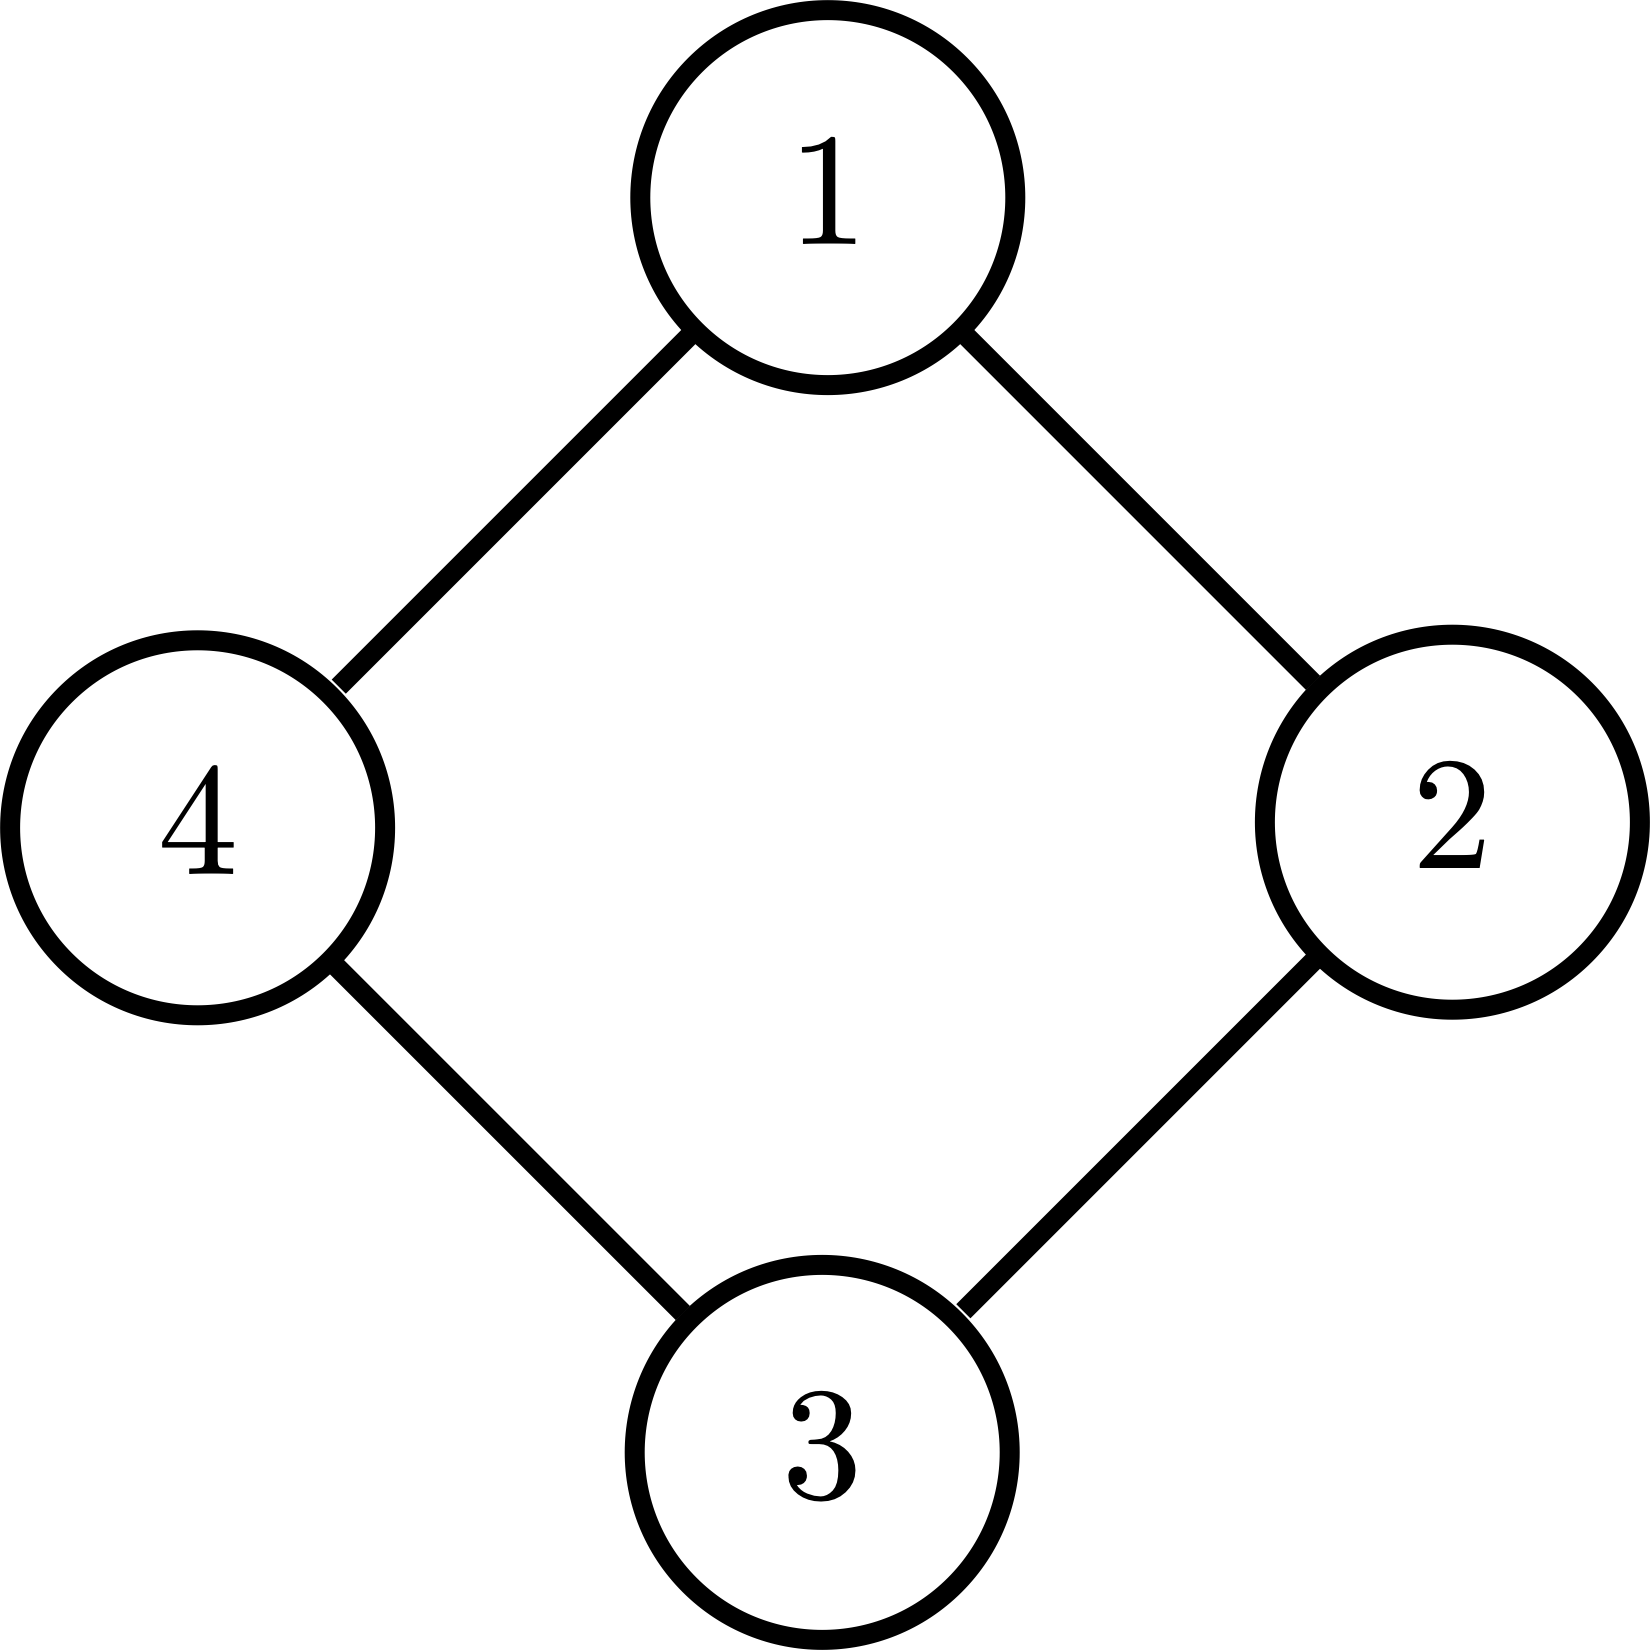
\includegraphics[width=3.5cm]{images/chapter9/LabelledSquare.png}}
	    \caption{Square With Labelled Corners}
	\end{figure}

    Let $X$ denote the set of colourings of the corners of the square, and let $G$ denote the rotation group acting on $X$. Then two elements of $X$ belong to the same orbit precisely when one is simply a rotation of the other. We note that $G$ consists of 4 rotations.
    \begin{enumerate}
        \item Rotating the square $0^\circ$ does not change the colourings at all, which means that the number of fixed points is the total number of possible colourings, which is $n^4$.
        \item Rotating the square $90^\circ$ results in all points affecting one another, so the only fixed points would be colourings of all the same color. Since there are $n$ different colours, thus the number of fixed points is $n$.
        \item Rotating the square $180^\circ$ swaps two pairs of vertices that are across from each other. Thus, a fixed point will occur if the two pairs have the same colour. hence, there are $n^2$ fixed points.
        \item Finally, rotating the square $270^\circ$ is similar to rotating $90^\circ$, so there are $n$ fixed points.
    \end{enumerate}
    Now there are 4 elements in $G$, so $|G| = 4$. By Burnside's Lemma,
    \[
        |X/G| = \frac{1}{|G|}\sum_{g\in G} |\Fix{X}{g}| = \frac14 (n^4 + n + n^2 + n),
    \]
    i.e., the number of distinct possible colourings of the corners on a square with $n$ colours (up to rotation) is $\frac n4 (n^3 + n + 2)$.
\end{example}

\section{Conjugacy Classes}
Before we look at the most important part of this chapter, the Class Equation, we look at the idea of conjugacy as a group action.
\begin{definition}
    Let $G$ be a group, and suppose $a, b \in G$. Then we say that $b$ is a \textbf{conjugate} of $a$ if there is an element $g \in G$ such that $b = gag^{-1}$ (or, alternatively, $a=g^{-1}bg$).
\end{definition}
We can frame this idea in terms of group actions.

Consider the function $\phi: G\times G\to G$ such that $\phi(g, x) = gxg^{-1}$. We showed that $\phi$ is a group action in \textbf{Exercise \ref{exercise-conjugacy-is-group-action}}. Let's look at the orbit and stabilizer of an arbitrary element $x \in G$ under this group action.
\begin{itemize}
    \item For orbits, we are to find $y \in G$ such that there exists a $g \in G$ such that $gxg^{-1} = y$. Hence, the orbit of $x$ under this group action are the conjugates of $x$.
    \item For the stabilizer, we are to find elements $g \in G$ such that $gxg^{-1} = x$. Hence we find $gx = xg$. Therefore, $g \in \C{G}{x}$ where $\C{G}{x}$ is the centralizer of $x$ (recall how it is defined in \textbf{Example \ref{example-centralizer-of-a-subset}}).
\end{itemize}

Hence, under the action of conjugation, $\Orb{G}{x} = \text{Conjugates of }x$, and $\Stab{G}{x} = \C{G}{x}$.

We can now look at conjugacy classes.
\begin{definition}
    Let $G$ be a group and take $x \in G$. The \textbf{conjugacy class of $x$} is the set
    \[
        \Cl{x} = \{gxg^{-1} \ | \ g \in G\}.
    \]
    In other words, the set $\Cl{x}$ is a subset of $G$ where all elements inside it are conjugates of each other.
\end{definition}
\begin{remark}
    We omit having the subscript of $G$ for the conjugacy class since $x \in G$. Also, under the group action of conjugation, $\Orb{G}{x} = \Cl{x}$.
\end{remark}

\begin{example}\label{example-conjugacy-classes-of-Sn3}
    We look at conjugacy classes of the group $\Sn{3}$.
    \begin{itemize}
        \item The first is the conjugacy class of the identity, $\id$.
        \[
            \Cl{\id} = \{g\circ\id\circ g^{-1} \ | \ g \in G \} = \{\id\}.
        \]
        Thus the conjugacy class of the identity consists of only the identity.
        \item The second is the conjugacy class of transpositions. Let $\tau = \begin{pmatrix}a & b\end{pmatrix}$ be a transposition in $\Sn{3}$. Then
        \[
            \Cl{\tau} = \{g\circ\tau\circ g^{-1} \ | \ g \in G\}.
        \]
        Running through all 6 elements of $\Sn{3}$ reveals that $\Cl{\tau}$ is the set of all transpositions, i.e. the conjugacy class of transpositions is the set of transpositions.
        \item The third is the conjugacy class of 3-cycles. Let $\sigma = \begin{pmatrix}a & b & c\end{pmatrix}$ be a 3-cycle in $\Sn{3}$. One can see that $\Cl{\sigma}$ is the set of all 3-cycles.
    \end{itemize}
\end{example}

\begin{exercise}\label{exercise-order-of-conjugacy-class}
    Let $G$ be a group and $x \in G$. Prove that
    \[
        |\Cl{x}| = [G : \C{G}{x}].
    \]
\end{exercise}

\section{The Class Equation}
The example of the previous section illustrates that the sum of the sizes of the conjugacy classes must be equal to the size of the group. This fact, along with the Orbit-Stabilizer theorem (\textbf{Theorem \ref{thrm-orbit-stabilizer}}), can be used to derive an important equation known as \textbf{the class equation}.

Before we state and prove the class equation, we recall the idea of the center of a group as introduced in \textbf{Example \ref{example-center-of-group}}.
\begin{quote}
    The center of a group $G$ is the normal subgroup
    \[
        \Z{G} = \{z \in G \ | \ gz = zg \text{ for all } g \in G\}.
    \]
    In other words, $\Z{G} = \{z \in G \ | \ z = gzg^{-1} \text{ for all } g \in G\}$.
\end{quote}

We now state and prove the class equation.
\begin{theorem}[Class Equation]\label{thrm-class-equation}
    Let $G$ be a finite group. Suppose $G$ has $k$ conjugacy classes, with $l$ of them having more than 1 element. Suppose $g_1, g_2, \dots, g_l$ are representatives of the conjugacy classes with more than 1 element. Then
    \[
        |G| = |\Z{G}| + \sum_{i=1}^l [G : \C{G}{g_i}],
    \]
    which is known as \textbf{the class equation}.
\end{theorem}

\begin{proof}
    We know by \textbf{Exercise \ref{exercise-distinct-orbits-partition-set}} that distinct orbits partitions the set that the group is acting on. Hence, using the group action of conjugation, orbits under conjugation partition $G$. Hence,
    \[
        G = \bigcup_{i=1}^k \Orb{G}{\hat{g_i}} = \bigcup_{i=1}^k \Cl{\hat{g_i}}
    \]
    where $\hat{g_i}$s are representatives of the $k$ conjugacy classes (including those with only 1 element).

    Suppose now that an element $x$ has a conjugacy class with one element. This means that $gxg^{-1} = x$ for all $g \in G$. Hence, this means that $x \in \Z{G}$.

    Therefore, one concludes that
    \[
        G = \left(\Z{G}\right) \cup \left(\bigcup_{i=1}^l \Cl{g_i}\right).
    \]
    Since this is a disjoint union, hence
    \[
        |G| = |\Z{G}| + \sum_{i=1}^l |\Cl{g_i}|.
    \]

    Finally, by \textbf{Exercise \ref{exercise-order-of-conjugacy-class}}, $|\Cl{g_i}| = [G : \C{G}{g_i}]$ which means that
    \[
        |G| = |\Z{G}| + \sum_{i=1}^l [G:\C{G}{g_i}],
    \]
    proving the theorem.
\end{proof}

We look at one application of the class equation. Before that, we introduce the idea of \textbf{$p$-groups}.
\begin{definition}
    A \textbf{$p$-group} $G$ is a finite group with order $p^n$ where $p$ is prime and $n$ is a positive integer.
\end{definition}
An immediate consequence of this is that every element must have an order that is a power of $p$, i.e. for any element $x \in G$, $|x| = p^k$ where $1 \leq k \leq n$.

\begin{example}\label{example-group-with-prime-power-order-has-non-trivial-center}
    Let $G$ be a finite $p$-group, meaning $|G| = p^n < \infty$. We will show that $G$ has a non-trivial center using the class equation.

    We recall that $|\Cl{x}| = \frac{|G|}{|\C{G}{x}|}$ by \textbf{Exercise \ref{exercise-order-of-conjugacy-class}}. Hence, the order of the group must divide the order of any conjugacy class, i.e. $\frac{|G|}{|\C{G}{x}|} \mid |G|$. Since $|G| = p^n$, it follows that $|\Cl{x}| = p^k$ for some $1 \leq k \leq n$ (assuming $x \notin \Z{G}$).

    If $g_1, g_2, \dots, g_l$ are representatives from the conjugacy classes with more than 1 element, then this means that
    \[
        p^n = |G| = |\Z{G}| + \sum_{i=1}^l |\Cl{g_i}| = |\Z{G}| + \sum_{i=1}^l p^{k_i}
    \]
    where $1 \leq k_1, k_2, \dots, k_l < n$. From this, we conclude that $p$ must divide $|\Z{G}|$, meaning $|\Z{G}| > 1$.
\end{example}
\begin{example}
    We look at the class equation of the symmetric group of degree 3, $\Sn{3}$.

    We recall from \textbf{Example \ref{example-conjugacy-classes-of-Sn3}} that the conjugacy classes of $\Sn{3}$ are
    \begin{align*}
        &\Cl{\id} = \{\id\}\\
        &\Cl{\tau} = \{\begin{pmatrix}1 & 2\end{pmatrix}, \begin{pmatrix}1 & 3\end{pmatrix}, \begin{pmatrix}2 & 3\end{pmatrix}\}\\
        &\Cl{\sigma} = \{\begin{pmatrix}1 & 2 & 3\end{pmatrix}, \begin{pmatrix}1 & 3 & 2\end{pmatrix}\}
    \end{align*}
    where $\tau$ is a 2-cycle (transposition) and $\sigma$ is a 3-cycle. Thus, the class equation of $\Sn{3}$ is
    \[
        6 = 1 + 2 + 3
    \]
    where $|\Z{\Sn{3}}| = |\{e\}| = 1$.
\end{example}

\begin{exercise}
    The Cayley table of $D_3$ is in \textbf{Example \ref{example-presentation-of-D3}}.
    \begin{enumerate}[label=(\alph*)]
        \item Find $\Z{D_3}$, the center of $D_3$.
        \item Find the conjugacy classes of $D_3$ with more than 1 element.
        \item Find the class equation of $D_3$.
    \end{enumerate}
\end{exercise}

\newpage

\section{Cauchy's Theorem}
To end this chapter, we prove \textbf{Cauchy's Group Theorem}.
\begin{theorem}[Cauchy]\label{thrm-cauchy}
    Let $G$ be a finite group such that $|G| = np$ where $p$ is a prime and $n$ is a positive integer. Then $G$ contains an element of order $p$.
\end{theorem}
\begin{proof}
    We proceed with strong induction on $n$.

    For the case where $n = 1$, $|G| = p$. Then by \textbf{Exercise \ref{exercise-prime-order-element}}, every element of the group has order $p$. Hence we proved the base case.

    We now assume that the statement holds for all $n \leq k$ for some positive integer $k$. We need to prove the case for $k+1$, that is, assuming that $|G| = (k+1)p$. We split the proof into two cases.

    The first case is when $G$ is abelian. Take any non-identity element $x$, and define $H = \langle x \rangle \leq G$.
    \begin{itemize}
        \item If $p$ divides $|H|$, say $|H| = mp$ where $m$ is a positive integer, then $x^m$ is an element of order $p$ (since $\left(x^m\right)^p = x^{|H|} = e$). Hence we find an element with order $p$.
        \item If $p$ does not divide $|H|$, then $p$ must divide $[G:H] = |G/H| = \frac{|G|}{|H|}$ since $p$ divides $|G| = kp$. Note that $H \lhd G$ since $G$ is abelian (\textbf{Proposition \ref{prop-subgroup-of-abelian-group-is-normal}}). Hence $G/H$ is a group. If $|x| = m$, then $(xH)^m = (x^m)H = eH = H \in G/H$. Thus, $m$ is a multiple of $|G/H|$ (\textbf{Corollary \ref{corollary-order-of-group-multiple-of-order-of-element}}) which is in turn a multiple of $p$. Hence $p$ divides $m$. As before, $x^{\frac mp}$ is an element with order $p$ (since $\left(x^{\frac mp}\right)^p = x^m = e$).
    \end{itemize}
    Therefore, for the abelian case, there exists an element with order equal to $p$.

    We now consider the case when $G$ is non-abelian. We assume by contradiction that $G$ does not have an element of order $p$. Let $H \leq G$ be a proper subgroup. By the assumption, $H$ has no element with order $p$. Therefore the contrapositive of the induction hypothesis means that $|H|$ is not a multiple of $p$. Note that Lagrange's Theorem (\textbf{Theorem \ref{thrm-lagrange}}) further explains that $|G| = [G:H]|H|$. Since $|H|$ is not divisible by $p$ and $|G|$ is divisible by $p$, we conclude that $p$ divides $[G:H]$ for every proper subgroup $H$.

    Since $G$ is non-abelian, $G \neq \Z{G}$ meaning that there are conjugacy classes with more than 1 element. Suppose there are $l$ such classes and let them be represented by $g_1, g_2, \dots, g_l$. By the class equation (\textbf{Theorem \ref{thrm-class-equation}}),
    \[
        |G| = |\Z{G}| + \sum_{i=1}^l [G:\C{G}{g_i}].
    \]
    Note that $|\Cl{g_i}| = [G:\C{G}{g_i}] = \frac{|G|}{|\C{G}{g_i}|} > 1$, which means that $|G| > |\C{G}{g_i}|$. Thus $\C{G}{g_i} \neq G$ for all $i$ since their orders are different. Recall that $\C{G}{g_i}$ is a proper subgroup of $G$, so by the above observation, $p$ divides $[G:\C{G}{g_i}]$.

    In the class equation, $p$ divides $|G|$ and $p$ divides $[G:\C{G}{g_i}]$, which means that $p$ must divide $|\Z{G}|$. But $\Z{G} \leq G$ and by above observation, $p$ does not divide any proper subgroup of $G$. Hence, $\Z{G} = \{e\}$ or $\Z{G} = G$. Note $\Z{G} \neq \{e\}$ because that would imply $p$ divides $1$ which is a contradiction. So $\Z{G} = G$, but that means that $G$ is abelian (\textbf{Problem \ref{problem-center-of-G}}) which is a contradiction. We thus conclude that there exists an element of order $p$.
\end{proof}

\begin{exercise}\label{exercise-group-of-order-multiple-of-prime-has-subgroup-of-prime-order}
    Let $G$ be a finite group with $|G| = np$, $n$ is a positive integer, and $p$ prime. Prove that $G$ has a \textbf{subgroup} of order $p$.
\end{exercise}

\newpage

\section{Problems}
\begin{problem}
    Let $G = D_5$, the dihedral group of order 10.
    \begin{enumerate}[label=(\alph*)]
        \item Suppose $H$ is a proper subgroup of $G$. What are the possible order(s) of $H$?
        \item For each of the possible order(s) identified, find such a subgroup.
    \end{enumerate}
\end{problem}

\begin{problem}
    Let $G$ be a group of order 25 and $X$ be a $G$-set of 24 elements. Show that every $g \in G$ has a fixed point.
\end{problem}

\begin{problem}
    Suppose $G$ is a finite group with order $n > 1$ where, for all $g \in G$, $g^2 = e$. Prove that $n = 2^k$ where $k$ is a positive integer.
\end{problem}

\begin{problem}
    A group action is said to be \textbf{free} if $g\cdot x = x$ implies that $g$ is the identity (i.e., only the identity fixes any $x$).\newline
    Let $G$ be a group and $S$ be a non-empty $G$-set. Suppose $G$ acts on $S$ freely and transitively. Prove that $G$ and $S$ have the same number of elements.
\end{problem}

\begin{problem}
    A bracelet consists of 3 beads that each can be one of $n$ colours. Two bracelets are considered to be identical if the rotation of one yields the other, or if one can be obtained via reflecting about a line, or any combination of these two actions. How many distinct bracelets are there?
\end{problem}

\begin{problem}\label{problem-group-of-order-prime-squared-is-abelian}
    Let $p$ be a prime number. Prove that a group of order $p^2$ must be abelian.\newline
    \textit{(Hint: Consider \textbf{Problem \ref{problem-center-of-G}} and \textbf{Problem \ref{problem-quotient-of-group-mod-center-is-cyclic-implies-abelian}})}
\end{problem}

\begin{problem}
    Let $G$ be a finite $p$-group, and $X$ be a $G$-set. Denote the set of points of $X$ that are fixed under the action of $G$ by $\Omega$. Prove that $|X| \equiv |\Omega| \pmod p$.\newline
    \textit{(Hint: $\Omega = \{x \in X \vert g\cdot x = x \textrm{ for all } g \in G\}$)}
\end{problem}

%=========================================
\chapter{Sylow Theorems}
The Sylow theorems are a collection of theorems named after the Norwegian mathematician Peter Ludwig Sylow that give detailed information about the number of subgroups of fixed order that a given finite group contains. The Sylow theorems form a fundamental part of finite group theory and have very important applications in the classification of finite simple groups.

\section{First Sylow Theorem}
Before we can state the First Sylow Theorem, we introduce some terminology.

Recall that a group with order $p^k$ for some $k \geq 0$ is called a $p$-group. If $G$ is a group with a subgroup of order $p^k$, then that subgroup is called a \textbf{$p$-subgroup}.
\begin{definition}\label{definition-sylow-p-subgroup}
    Let $G$ be a finite group. Write the order of the group $G$ as $p^k m$ where $p$ is prime, $k \geq 0$, and $p \nmid m$. Then a subgroup $H$ with order $p^k$ is called a \textbf{Sylow $p$-subgroup} of $G$.
\end{definition}
We denote the set of all Sylow $p$-subgroups of the group $G$ for a given prime $p$ by $\Syl{p}{G}$.

\begin{exercise}
    Find the Sylow 2-subgroup of $\mathbb{Z}_{12}$.
\end{exercise}

\newpage

We are now ready to state and prove the \textbf{First Sylow Theorem}.
\begin{theorem}[Sylow I]\label{thrm-sylow-1}
    Let $G$ be a finite group with order $p^k m$ where $p$ is prime, $k \geq 0$, and $p \nmid m$. Then $\Syl{p}{G} \neq \emptyset$.
\end{theorem}
\begin{remark}
    Equivalently, for a finite group $G$, for every prime factor $p$ with multiplicity $k$ of its order, there is a Sylow $p$-subgroup of $G$.
\end{remark}
\begin{proof}[Proof (see {\cite[pp.~1--3]{mann_2011}})]
    We induct on the order of $G$.

    When the order of $G$ is 1, $|G| = p^0$ for any prime $p$, so $G$ is clearly a Sylow $p$-subgroup of itself.

    We assume now that the theorem holds for all groups of order strictly less than $n$, meaning that for any group $H$ with order $p^k m < n$, $\Syl{p}{H} \neq \emptyset$. We need to prove the case where the group has order $n$. We write $n = p^k m$ where $p$ is prime, $k \geq 1$, and $p \nmid m$. We split the argument into two separate cases.

    The first case is when $p$ divides the order of the center of $G$, $|\Z{G}|$. By Cauchy's Theorem (\textbf{Theorem \ref{thrm-cauchy}}), $\Z{G}$ contains a subgroup of order $p$, say $N$. We note that $N \lhd G$ since for all $x \in N \subseteq \Z{G}$ and $g \in G$, $gxg^{-1} = (gx)g^{-1} = x(gg^{-1}) = x \in N$. Hence $G/N$ is a group, and it has order $\frac np = \frac{p^km}{p} = p^{k-1}m$. Since $p^{k-1}m < p^km = n$, thus by the Inductive Hypothesis $G/N$ has a Sylow $p$-subgroup, say $\bar{S}$, meaning that $\bar{S} \leq G/N$ has order $p^{k-1}$.

    We now construct the group $S = \{g \in G \vert gN \in \bar{S}\}$ under the group operation of $G$. Clearly $S$ is non-empty since $e \in S$ (as $eN = N \in \bar{S} \leq G/N$). Suppose $g_1, g_2 \in S$, meaning that $g_1N, g_2N \in \bar{S}$. Therefore $(g_1g_2^{-1})N = (g_1N)(g_2N)^{-1} \in \bar{S}$ which implies that $g_1g_2^{-1} \in S$. By the subgroup test, $S \leq G$. Also, $N \leq S$ since for all $n \in N$, $nN = N \in \bar{S}$.

    We construct the homomorphism $\phi: S \to \bar{S}$ such that $g \mapsto gN$. By construction one sees clearly that $\phi$ is surjective, meaning that $\im \phi = \bar{S}$. Furthermore,
    \begin{align*}
        \ker\phi &= \{s \in S \vert \phi(s) = N\}\\
        &= \{s \in S \vert sN = N \}\\
        &= \{s \in S \vert s \in N \}\\
        &= S \cap N\\
        &= N & (\text{since } N \leq S).
    \end{align*}
    By the Fundamental Homomorphism Theorem (\textbf{Theorem \ref{thrm-first-isomorphism}}), $S/N \cong \bar{S}$, meaning that $p^{k-1} = |\bar{S}| = \frac{|S|}{|N|} = \frac{|S|}{p}$ which quickly implies that $|S| = p^k$. Hence, there exists a $S \leq G$ such that $|S| = p^k$, meaning that $S$ is a Sylow $p$-subgroup of $G$.

    We can now start on the second case where $p$ does not divide the order of the center of $G$. We recall the class equation (\textbf{Theorem \ref{thrm-class-equation}})
    \[
        |G| = |\Z{G}| + \sum_{i=1}^l [G:\C{G}{g_i}].
    \]
    where $g_1, g_2, \dots, g_l$ are representatives of the $l$ distinct conjugacy classes with more than one element. We note that $p$ divides $|G|$. Since $p$ does not divide $|\Z{G}|$ in this case, thus $\sum_{i=1}^l [G:\C{G}{g_i}]$ must also not divide $p$ in order for their sum to be divisible by $p$. Hence, there is at least one conjugacy class with more than one element such that $p$ does not divide $[G:\C{G}{g_i}]$. We note that $[G:\C{G}{g_i}] = \frac{|G|}{|\C{G}{g_i}|}$ by Lagrange's Theorem (\textbf{Theorem \ref{thrm-lagrange}}). Therefore, if $p$ does not divide $\frac{|G|}{|\C{G}{g_i}|} = \frac{p^k m}{|\C{G}{g_i}|}$, then we conclude that $|\C{G}{g_i}| = p^ka$ for some $a$.

    We now argue that $a < m$ (recalling that $|G| = p^km$). Clearly $a \leq m$ since if $a > m$ then $\frac{p^k m}{|\C{G}{g_i}|}$ is not an integer. If instead $a = m$ then $|\C{G}{g_i}| = p^km = |G|$, and since $\C{G}{g_i} \leq G$ with them having equal orders, we conclude $G = \C{G}{g_i}$. This means that every element in $G$ commutes with $g_i$, which quickly implies $g_i \in \Z{G}$. But an element is in $\Z{G}$ if its conjugacy class has only one element, which is not the case. Hence $a \neq m$, meaning that $a < m$.

    In summary, $\C{G}{g_i} \leq G$ with $|\C{G}{g_i}| = p^ka < p^km = n$. Therefore we apply the Induction Hypothesis on $\C{G}{g_i}$ to say that $\C{G}{g_i}$ has a Sylow $p$-subgroup of order $p^k$. Clearly a subgroup of $\C{G}{g_i}$ has to also be a subgroup of $G$, meaning that $G$ has a Sylow $p$-subgroup.

    Therefore, any finite group $G$ with order written as $p^k m$ has a Sylow $p$-subgroup, meaning that $\Syl{p}{G} \neq \emptyset$.
\end{proof}

\begin{exercise}
    Find the set of primes $p$ such that $\Syl{p}{\Sn{5}} \neq \emptyset$.
\end{exercise}

\section{Conjugate Subgroup}
Before we look at the next Sylow theorem, we need to introduce two more things. The first is the notion of the \textbf{conjugate subgroup}.
\begin{definition}
    Let $G$ be a group, $H \leq G$, and $g \in G$. Then the \textbf{conjugate subgroup of $H$ by $g$} is
    \[
        gHg^{-1} = \{ghg^{-1} \vert h \in H\}.
    \]
    under the group operation of $G$.
\end{definition}
We proved that $gHg^{-1}$ is a subgroup of $G$ in \textbf{Exercise \ref{exercise-conjugate-subgroup}}.

\begin{exercise}\label{exercise-conjugate-subgroup-isomorphic-to-subgroup}
    Let $G$ be a group and $H \leq G$. Prove that $gHg^{-1} \cong H$ for any $g \in G$.
\end{exercise}

We prove some results regarding the conjugate subgroup here.
\begin{proposition}\label{prop-power-of-conjugate-equals-conjugate-of-power}
    Let $G$ be a group, and let $x$ and $y$ be elements in $G$ such that there exists an element $a \in G$ such that $y = axa^{-1}$. Then $y^n = ax^na^{-1}$ for all integers $n$.
\end{proposition}
\begin{proof}
    Trivially, when $n = 0$, $y^0 = e = y^0 = x^0 = ax^0a^{-1}$.

    We consider a proof by induction for positive integers $n$ and then prove the negative case.

    When $n = 1$, $y = axa^{-1}$ is given. Now assume $n = k$ holds true for some positive integer $k$, meaning that $y^k = ax^ka^{-1}$. We will prove that $y^{k+1} = ax^{k+1}a^{-1}$.
    \begin{align*}
        y^{k+1} &= y(y^k)\\
        &= (axa^{-1})(ax^ka^{-1}) & (\text{Induction Hypothesis})\\
        &= axa^{-1}ax^ka^{-1}\\
        &= axx^ka^{-1}\\
        &= ax^{k+1}a^{-1}
    \end{align*}
    which completes this induction for positive integers $n$.

    Now suppose $n$ is a non-negative integer. Then
    \begin{align*}
        y^{-n} &= (y^n)^{-1}\\
        &= (ax^na^{-1})^{-1} & (\text{by above result})\\
        &= a(x^n)^{-1}a^{-1}\\
        &= ax^{-n}a^{-1}
    \end{align*}
    which completes the proof for all integers.
\end{proof}

\begin{proposition}\label{prop-order-of-conjugate-element equals-order-of-element}
    Let $G$ be a group. Then for all $g, x \in G$, we have $|gxg^{-1}| = |x|$.
\end{proposition}
\begin{proof}
    The proposition trivially holds true for $g = e$ so we assume $g \neq e$.

    Suppose $|x| = n$, meaning $x^n = e$ and $x^k \neq e$ for all $1 \leq k < n$. Note we have
    \begin{align*}
        (gxg^{-1})^n  &= gx^ng^{-1} & (\textbf{Proposition \ref{prop-power-of-conjugate-equals-conjugate-of-power}})\\
        &= geg^{-1} & (\text{since } |x| = n)\\
        &= e
    \end{align*}
    which means that $|gxg^{-1}| \leq n = |x|$.

    Now consider $(gxg^{-1})^k = gx^kg^{-1}$. Suppose $k$ is a positive integer such that $x^k = h$ where $h \neq e$. Then $gx^kg^{-1} = ghg^{-1}$. We argue that $ghg^{-1} \neq e$.
    \begin{itemize}
        \item If $gh = e$ then $gx^kg^{-1} = g^{-1} \neq e$ since $g \neq e$.
        \item If instead $hg^{-1} = e$ then $gx^kg^{-1} = g \neq e$.
    \end{itemize}
    Hence, if $x^k \neq e$, then $(gxg^{-1})^k = gx^kg^{-1} \neq e$, meaning that $|x| \leq |gxg^{-1}|$.

    Therefore $|gxg^{-1}| = |x|$.
\end{proof}

\begin{exercise}
    Prove that for any group $G$, $|gh| = |hg|$ for all $g, h \in G$.
\end{exercise}

We note an important result with regards to the conjugate subgroup.
\begin{theorem}\label{thrm-unique-subgroup-of-given-order-is-normal}
    Let $G$ be a group. Suppose $H$ is the only subgroup of $G$ with a given order. Then $H \lhd G$.
\end{theorem}
\begin{proof}
    Suppose $g \in G$. By \textbf{Exercise \ref{exercise-conjugate-subgroup-isomorphic-to-subgroup}} we know $gHg^{-1} \cong H$ which means that $|gHg^{-1}| = |H|$. Furthermore, by \textbf{Exercise \ref{exercise-conjugate-subgroup}} we know that $gHg^{-1} \leq G$. Since $H$ is the only subgroup of that order (by assumption), we conclude that $gHg^{-1} = H$, which quickly means that $H \lhd G$ by definition of a normal subgroup.
\end{proof}

\newpage

\section{The Normalizer}
We now look at the definition of the \textbf{normalizer}.
\begin{definition}
    Let $G$ be a group and $S$ be a subset of $G$. The \textbf{normalizer of $S$ in $G$} is given by
    \[
        \N{G}{S} = \{g \in G \vert gS = Sg \}.
    \]
\end{definition}
\begin{remark}
    Equivalently, $\N{G}{S} = \{g \in G \vert gSg^{-1} = S \}$.
\end{remark}
\begin{exercise}\label{exercise-normalizer-is-subgroup-of-main-group}
    Let $G$ be a group and $S$ be a subset of $G$. Prove that $\N{G}{S} \leq G$.
\end{exercise}

We prove some properties of the normalizer here.
\begin{proposition}\label{prop-subgroup-is-a-normal-subgroup-of-normalizer}
    Let $G$ be a group, and $H \leq G$. Then $H \lhd \N{G}{H}$.
\end{proposition}
\begin{proof}
    We first prove $H \leq \N{G}{H}$ and then prove normality.

    We know that both $H$ and $\N{G}{H}$ are subgroups of $G$, so both are groups. We just need to check that $H \subseteq \N{G}{H}$ to prove that $H \leq \N{G}{H}$.

    Consider any $h \in H$. We note that $hH = H$ and $Hh^{-1} = H$ since $h^{-1} \in H$. Thus, if $h \in H$, then
    \[
        hHh^{-1} = h(Hh^{-1}) = hH = H
    \]
    which means that $h \in \N{G}{H}$ by definition of the normalizer. Hence any element in $H$ is also an element of $\N{G}{H}$, meaning $H \subseteq \N{G}{H}$.

    It follows then that $H \leq \N{G}{H}$ since $H \subseteq \N{G}{H}$ and $H$ is a group.

    Now we prove normality. Consider any $n \in \N{G}{H}$, which means that $nHn^{-1} = H$. This immediately implies that $H \lhd \N{G}{H}$.
\end{proof}
\begin{remark}
    Combining the results from \textbf{Exercise \ref{exercise-normalizer-is-subgroup-of-main-group}} and \textbf{Proposition \ref{prop-subgroup-is-a-normal-subgroup-of-normalizer}} means that $H \lhd \N{G}{H} \leq G$.
\end{remark}

\begin{proposition}\label{prop-normalizer-of-subgroup-is-largest-subgroup-containing-that-subgroup-as-a-normal-subgroup}
    Let $G$ be a group, and $H \leq G$. Then $\N{G}{H}$ is the largest subgroup of $G$ containing $H$ as a normal subgroup.
\end{proposition}
\begin{remark}
    What we mean by ``largest'' here is that if there was another subgroup of $G$, say $K$, that permits $H \lhd K$, then it must be the case that $K \subseteq \N{G}{H}$.
\end{remark}
\begin{proof}
    By \textbf{Proposition \ref{prop-subgroup-is-a-normal-subgroup-of-normalizer}} we know that $H \lhd \N{G}{H}$. We just need to prove that any subgroup in which $H$ is normal inside it must be a subset of $\N{G}{H}$.

    Consider any subgroup $N \leq G$ such that $H \lhd N \leq G$. Then for any $n \in N$ we have $nHn^{-1} = H$ by definition of normality, which immediately means that $n \in \N{G}{H}$ by definition of the normalizer of $H$ in $G$. Hence any element in $N$ also belongs in $\N{G}{H}$, meaning $N \subseteq \N{G}{H}$.

    This completes the proof that $\N{G}{H}$ is the largest subgroup of $G$ that contains $H$ as a normal subgroup.
\end{proof}

\begin{proposition}\label{prop-normalizer-of-sylow-p-subgroup}
    Let $G$ be a finite group. Let $P$ be a Sylow $p$-subgroup of $G$, and $Q$ be a $p$-subgroup of $\N{G}{P}$. Then $Q \subseteq P$. In particular, if $Q$ is a Sylow $p$-subgroup of $\N{G}{P}$, then $P = Q$.
\end{proposition}
\begin{proof}[Proof (see {\cite[Proposition 11.9]{humphreys_1996}})]
    For brevity, write the order of $G$ as $xp^n$ where $p \nmid x$, $|P| = p^n$, and $|Q| = p^m$.

    Recall by the Diamond Isomorphism Theorem (\textbf{Theorem \ref{thrm-second-isomorphism}}), statement 3, we have $PQ \leq \N{G}{P}$ since $P \lhd \N{G}{P}$ by \textbf{Proposition \ref{prop-subgroup-is-a-normal-subgroup-of-normalizer}}. As $\N{G}{P} \leq G$ thus $PQ \leq G$. In addition, by \textbf{Exercise \ref{exercise-order-of-subgroup-product}},
    \[
        |PQ| = \frac{|P||Q|}{|P \cap Q|} = p^{n+m-s}
    \]
    where we define $|P \cap Q| = p^s$. By Lagrange's Theorem (\textbf{Theorem \ref{thrm-lagrange}}) we know that $|G| = a|PQ|$ so $p^n = ap^{n+m-s}$ which implies $1 = ap^{m-s}$. Since $a$ is a positive integer, thus $p^{m-s} = \frac 1a$ which means $m \leq s$.

    We note by \textbf{Problem \ref{problem-intersection-of-subgroups}}, $P \cap Q \leq Q$, meaning $|Q| = b|P\cap Q|$ by Lagrange's Theorem. Thus $p^m = bp^s$ which implies $p^{m-s} = b \geq 1$ so $m \geq s$.

    Hence $m = s$ which means $|P \cap Q| = |Q|$, i.e. $P \cap Q = Q$. Therefore $Q \subseteq P$ which is the first part of the proposition proved.

    Now suppose $Q$ is, in particular, a Sylow $p$-subgroup of $\N{G}{P}$. Since $\N{G}{P} \leq G$ by \textbf{Exercise \ref{exercise-normalizer-is-subgroup-of-main-group}}, one concludes that $|G| = y|\N{G}{P}|$ by Lagrange's Theorem. Hence $xp^n = y|\N{G}{P}|$ which implies $|\N{G}{P}| = \frac{x}{y} p^n = zp^n$ where $z = \frac xy$ and one observes $p \nmid z$. Therefore, if $Q$ is a Sylow $p$-subgroup, then $|Q| = p^n = |P|$ which implies $P = Q$ as $Q \subseteq P$.
\end{proof}

\section{Second Sylow Theorem}
We can now look at the \textbf{Second Sylow Theorem}.
\begin{theorem}[Sylow II]\label{thrm-sylow-2}
    Let $G$ be a finite group and $p$ be a prime number. Suppose $H$ and $K$ are both Sylow $p$-subgroups of $G$. Then there exists an element $g \in G$ such that $gHg^{-1} = K$.
\end{theorem}
\begin{proof}[Proof (see {\cite[Theorem 11.10]{humphreys_1996}} and {\cite[pp.~3--5]{mann_2011}})]
    Let $H$ be a Sylow $p$-subgroup of $G$. Define the set
    \[
        \mathcal{X} = \{gHg^{-1} \vert g \in G\}
    \]
    and denote an element from $\mathcal{X}$ by $X$.

    Let the Sylow $p$-subgroup $H$ act on $\mathcal{X}$ by conjugation, meaning $h \cdot X = hXh^{-1}$. We prove that this is, in fact, a group action.
    
    \begin{itemize}
        \item \textbf{Closure}: We have to prove closure because it is not implicit in the definition of this action.

        Let $X = gHg^{-1}$ for some $g \in G$. Then
        \[
            h\cdot X = hHh^{-1} = hgHg^{-1}h^{-1} = (hg)H(hg)^{-1}.
        \]
        Since $h \in H \leq G$, then $hg \in G$, which thus means that $h \cdot X = (hg)H(hg)^{-1} \in \mathcal{X}$.
        \item \textbf{Identity}: $e \cdot X = eXe^{-1} = X$.
        \item \textbf{Compatibility}: Let $h_1, h_2 \in H$. Then
        \begin{align*}
            h_1 \cdot (h_2 \cdot X) &= h_1 \cdot (h_2Xh_2^{-1})\\
            &= h_1h_2Xh_2^{-1}h_1^{-1}\\
            &= (h_1h_2)X(h_1h_2)^{-1}\\
            &= (h_1h_2) \cdot X.
        \end{align*}
    \end{itemize}

    We consider the orbits of this group action. We note that $\Orb{H}{H} = \{X \in \mathcal{X} \vert h \cdot H = H \text{ for some } h \in H\}$ and $h\cdot H = hHh^{-1} = P$ since $h \in H$. Thus $\Orb{H}{H} = \{H\}$, meaning $|\Orb{H}{H}| = 1$. We now show that $X = H$ is the only element in $\mathcal{X}$ such that $|\Orb{H}{X}| = 1$. If $X$ has one element in its orbit, then for all $h \in H$, $h\cdot X = hXh^{-1} = X$. Since $X = gHg^{-1}$ for some $g$, thus
    \begin{align*}
        &h(gHg^{-1})h^{-1} = gHg^{-1}\\
        \iff&hgHg^{-1} = gHg^{-1}h\\
        \iff&hgH = gHg^{-1}hg\\
        \iff&(g^{-1}hg)H = H(g^{-1}hg)\\
        \iff&g^{-1}hg \in \N{G}{H}.
    \end{align*}
    By \textbf{Proposition \ref{prop-order-of-conjugate-element equals-order-of-element}}, $|g^{-1}hg| = |h|$, and since the order of $H$ is $p^k$, thus for all elements $g^{-1}hg \in X$, they have order $p^k$. By definition of a $p$-group, one sees that $g^{-1}Hg$ is a $p$-subgroup of $\N{G}{H}$. Now clearly $g^{-1}Hg \cong H$ (by making the substitution $h = g^{-1}$ and then using \textbf{Exercise \ref{exercise-conjugate-subgroup-isomorphic-to-subgroup}} result) which means that $g^{-1}Hg$ has the same number of elements as $H$. Hence, $g^{-1}Hg$ is a Sylow $p$-subgroup of $\N{G}{H}$. Therefore by \textbf{Proposition \ref{prop-normalizer-of-sylow-p-subgroup}},  $H = g^{-1}Hg$, which means $X = gHg^{-1} = H$. Hence $H$ is the only element of $\mathcal{X}$ with $|\Orb{H}{X}| = 1$. Therefore for any $g \notin H$, $|\Orb{H}{gHg^{-1}}| > 1$. In fact, by Orbit-Stabilizer Theorem (\textbf{Theorem \ref{thrm-orbit-stabilizer}}), one sees that
    \[
        |\Stab{H}{gHg^{-1}}| = \frac{|H|}{|\Orb{H}{gHg^{-1}}|}
    \]
    and since $|H|$ is a power of $p$ and $|\Stab{H}{gHg^{-1}}|$ is an integer, thus $|\Orb{H}{gHg^{-1}}|$ has to be a power of $p$, meaning $|\Orb{H}{gHg^{-1}}| \equiv 0 \pmod p$. Because distinct orbits partition $\mathcal{X}$ (\textbf{Exercise \ref{exercise-distinct-orbits-partition-set}}), thus $|\mathcal{X}| \equiv 1 \pmod p$.

    Now let the Sylow $p$-subgroup $K$ act on $\mathcal{X}$ by conjugation, meaning $k \star X = kXk^{-1}$. This is a group action as proven before, and the above conclusion means that there is at least one orbit of length 1. Hence there exists a $g \in G$ such that for all $k \in K$, we have $k(gHg^{-1})k^{-1} = gHg^{-1}$. Hence $g^{-1}kg \in \N{G}{H}$ which means $g^{-1}Kg \subset \N{G}{H}$. Therefore, since $|K| = |g^{-1}Kg|$ and by \textbf{Proposition \ref{prop-normalizer-of-sylow-p-subgroup}}, $g^{-1}Kg \subseteq H$, meaning $K \subseteq gHg^{-1}$. But because $|H| = |K|$ as they are both Sylow $p$-subgroups, therefore $K = gHg^{-1}$.
\end{proof}
\begin{remark}
    What part of this proof shows is that if $P$ is a Sylow $p$-subgroup but $Q$ is only a $p$-subgroup, then $Q \subseteq gPg^{-1}$ for some $g \in G$.
\end{remark}

We note one important corollary of the Second Sylow Theorem.
\begin{corollary-thrm}\label{corollary-sylow-subgroup-is-normal-if-it-is-unique}
    Let $G$ be a finite group and $P$ be a Sylow $p$-subgroup for some prime $p$. Then $P$ is a normal subgroup of $G$ if and only if $P$ is the only Sylow $p$-subgroup of $G$.
\end{corollary-thrm}
\begin{proof}
    The reverse direction is easy to prove. Since $P$ is the only Sylow $p$-subgroup of $G$, this means that $P$ is the only subgroup of order $p^k$. By \textbf{Theorem \ref{thrm-unique-subgroup-of-given-order-is-normal}}, this means that $P \lhd G$.

    We work on the forward direction now and suppose $P$ is a normal subgroup of $G$. Let $\hat{P}$ be a normal Sylow $p$-subgroup. By the Second Sylow Theorem (\textbf{Theorem \ref{thrm-sylow-2}}), there exists $g \in G$ such that $g\hat{P}g^{-1} = P$. But since $\hat{P}$ is normal, thus $g^{-1}\hat{P}g = \hat{P}$ by definition of normality. Hence, $P = \hat{P}$, meaning that there is only one Sylow $p$-subgroup.
\end{proof}

\begin{exercise}
    Let $G$ be a finite group, $p$ be a prime number, and $H$ and $K$ be distinct Sylow $p$-subgroups of $G$. Prove that $H \cong K$.
\end{exercise}

\section{Third Sylow Theorem}
We now state and prove the \textbf{Third Sylow Theorem}.
\begin{theorem}[Sylow III]\label{thrm-sylow-3}
    Let $G$ be a finite group with order $p^k m$ where $p$ is prime, $k \geq 1$, and $p \nmid m$. Let $n_p$ denote the number of Sylow $p$-subgroups in $G$, i.e. $n_p = |\Syl{p}{G}|$. Then,
    \begin{enumerate}
        \item $n_p = [G:\N{G}{P}]$, where $P$ is a Sylow $p$-subgroup of $G$;
        \item $n_p$ divides $m$; and
        \item $n_p \equiv 1 \pmod p$.
    \end{enumerate}
\end{theorem}
\begin{proof}[Proof (adapted from \cite{wielandt_1959})]
    We prove the three statements in order.
    \begin{enumerate}
        \item Let $G$ act on $\Syl{p}{G}$ by conjugation, meaning that for any $g \in G$ and $P \in \Syl{p}{G}$, $g\cdot P = gPg^{-1}$. By the Second Sylow Theorem (\textbf{Theorem \ref{thrm-sylow-2}}), all Sylow $p$-subgroups are conjugates of each other, so the orbit of any $P \in \Syl{p}{G}$ is the set of all Sylow $p$-subgroups, meaning $|\Orb{G}{P}| = |\Syl{p}{G}| = n_p$. Now consider $\Stab{G}{P}$; note
        \[
            \Stab{G}{P} = \{g \in G \vert gPg^{-1} = P\} = \N{G}{P}
        \]
        by definition of the normalizer. By the Orbit-Stabilizer Theorem (\textbf{Theorem \ref{thrm-orbit-stabilizer}}),
        \[
            n_p = |\Orb{G}{P}| = \frac{|G|}{|\Stab{G}{P}|} = \frac{|G|}{|\N{G}{P}|} = [G : \N{G}{P}]
        \]
        by Lagrange's Theorem (\textbf{Theorem \ref{thrm-lagrange}}) and we are done.

        \item Let $P$ be a Sylow $p$-subgroup. We recall that $P \lhd \N{G}{P} \leq G$. Note that by Lagrange's Theorem we know $|\N{G}{P}| = [\N{G}{P} : P]|P| = ap^k$ where $a \leq m$ (since $\N{G}{P} \leq G$). Furthermore
        \[
            mp^k = |G| = [G: \N{G}{P}]|\N{G}{P}| = n_p(ap^k)
        \]
        which means $m = an_p$. In other words, $n_p$ divides $m$.

        \item Let $H$ be a Sylow $p$-subgroup and let it act on $\Syl{p}{G}$ by conjugation, meaning that for any $h \in H$ and $P \in \Syl{p}{G}$, $h \cdot P = hPh^{-1}$. Let $\Omega$ denote the set of fixed points of $\Syl{p}{G}$ under this action.

        Suppose $Q \in \Omega$, which means that $hQh^{-1} = Q$ for all $h \in H$. Thus $H \subseteq \N{G}{Q}$ as $\N{G}{Q} = \{g \in G \vert gQg^{-1} = Q\}$. In fact, since $H$ is a Sylow $p$-subgroup, $H \leq \N{G}{Q}$. We note $Q \lhd \N{G}{Q}$ by \textbf{Proposition \ref{prop-subgroup-is-a-normal-subgroup-of-normalizer}}. Hence $H$ and $Q$ are Sylow $p$-subgroups of $\N{G}{Q}$, which means there exists $n \in \N{G}{Q}$ such that $nQn^{-1} = H$ by the Second Sylow Theorem (\textbf{Theorem \ref{thrm-sylow-2}}). Furthermore $nQn^{-1} = Q$ since $Q \lhd \N{G}{Q}$. Hence $Q = H$ which means that the only element in $\Omega$ is $H$.

        By a similar argument posed in the proof of the Second Sylow Theorem, for any $Q \in \Syl{p}{G}$ where $Q \neq H$ we must have $|\Orb{H}{Q}| \equiv 0 \pmod p$. Note $|\Orb{H}{H}| = 1$. Now since distinct orbits partition $\Syl{p}{G}$, we must have $n_p = |\Syl{p}{G}| \equiv 1 \pmod p$.
    \end{enumerate}
    This completes the proof of the Third Sylow Theorem.
\end{proof}

\begin{example}
    We will show that a group of order 4225 is abelian by using the Third Sylow Theorem and other results.

    Note that $4225 = 5^2 \times 13^2$. Let $G$ be a group of order 4225. By the Third Sylow Theorem (\textbf{Theorem \ref{thrm-sylow-3}}), we know that
    \begin{itemize}
        \item $n_5 \mid 13^2 = 169$ and $n_{13} \mid 5^2 = 25$, which means $n_5 \in \{1, 13, 169\}$ and $n_{13} \in \{1, 5, 25\}$; and
        \item $n_5 \equiv 1 \pmod 5$ and $n_{13} \equiv 1 \pmod{13}$, which means $n_5 \in \{1, 6, 11, \dots\}$ and $n_{13} \in \{1, 14, 27, \dots\}$.
    \end{itemize}
    Hence, $n_5 = 1$ and $n_{13} = 1$, meaning that there is only one Sylow 5-subgroup and one Sylow 13-subgroup.

    Let $P$ be the Sylow 5-subgroup and $Q$ be the Sylow 13-subgroup. By \textbf{Corollary \ref{corollary-sylow-subgroup-is-normal-if-it-is-unique}}, $P \lhd G$ and $Q \lhd G$, so $pq = qp$ for any $p \in P$ and $q \in Q$. Furthermore, by \textbf{Problem \ref{problem-intersection-of-coprime-subgroups}}, $P \cap Q = \{e\}$. Finally, notice that
    \[
        |PQ| = \frac{|P||Q|}{|P\cap Q|} = |P||Q| = 5^2\times13^2 = |G|
    \]
    which means that $PQ$ and $G$ have the same number of elements. Hence, $G$ is the internal direct product of $P$ and $Q$. We note that
    \[
        G = PQ \cong P\times Q
    \]
    by direct product equivalence (\textbf{Theorem \ref{thrm-direct-product-equivilance}}). In addition, since $P$ and $Q$ are groups of prime-squared order, they are abelian (\textbf{Problem \ref{problem-group-of-order-prime-squared-is-abelian}}), meaning that their external direct product $P\times Q$ is also abelian (\textbf{Problem \ref{problem-external-direct-product-of-abelian-groups-is-abelian}}). Hence $G$ is also abelian since $G \cong P \times Q$.
\end{example}

\begin{exercise}
    Let $G$ be a group of order 784, and let $P$ be a Sylow 7-subgroup that is \textbf{not} a normal subgroup of $G$. Find the order of $\N{G}{P}$.
\end{exercise}

\section{Testing Non-Simplicity Of Groups}
To end this chapter, we look at the idea of \textbf{simple groups} and devise a test to prove the non-simplicity of groups.
\begin{definition}
    Let $G$ be a non-trivial group. Then $G$ is \textbf{simple} if the only normal subgroups of $G$ are the identity and $G$ itself.
\end{definition}
\begin{remark}
    Equivalently, $G$ is simple if $G$ has no proper normal subgroups.
\end{remark}

We may use part of the Third Sylow Theorem to create a test for non-simplicity.
\begin{theorem}[Sylow's Test]
    Let $n$ be a non-prime integer and let $p$ be a prime divisor of $n$. If 1 is the only divisor of $n$ that is congruent 1 modulo $p$, then there does not exist a simple group of order $n$.
\end{theorem}
\begin{proof}
    We first suppose $n = p^k$ where $k > 1$. Let $G$ be a group of order $n$. We consider two cases.
    \begin{itemize}
        \item Suppose $G$ is abelian. By writing $p^k$ as $p \times p^{k-1}$, a corollary of Cauchy's Theorem (\textbf{Exercise \ref{exercise-group-of-order-multiple-of-prime-has-subgroup-of-prime-order}}) tells us that there exists a subgroup of order $p$. Since every subgroup of an abelian group is normal (\textbf{Propopsition \ref{prop-subgroup-of-abelian-group-is-normal}}), thus there exists a proper normal subgroup of $G$, meaning $G$ is non-simple.
        \item Suppose now $G$ is non-abelian. By \textbf{Example \ref{example-group-with-prime-power-order-has-non-trivial-center}}, $G$ has a non-trivial center. Furthermore, $G \neq \Z{G}$ because $G$ is non-abelian (\textbf{Problem \ref{problem-center-of-G}}). Since the center is a normal subgroup of $G$, it is thus a proper normal subgroup of $G$, meaning $G$ is non-simple.
    \end{itemize}
    Hence any group of order $p^k$ where $k > 1$ is non-simple.

    Now suppose $n$ is not a prime power. By the Third Sylow Theorem (\textbf{Theorem \ref{thrm-sylow-3}}), the number of Sylow $p$-subgroups, $n_p$, is congruent to 1 modulo $p$ and divides $n$. Since 1 is the only such number by our assumption, thus $n_p = 1$, meaning that there is only one Sylow $p$-subgroup. By \textbf{Corollary \ref{corollary-sylow-subgroup-is-normal-if-it-is-unique}} this means that that Sylow $p$-subgroup (which is non-trivial) is normal, which thus means that any group of order $n$ is non-simple.
\end{proof}
\begin{example}
    Consider a group with order 15. Note $15 = 3 \times 5$, and consider $p = 5$. The divisors of 15 are 1, 3, 5, and 15, and clearly only 1 is congruent to 1 modulo 5. Hence by Sylow's Test we know that a group of order 15 cannot be simple.
\end{example}

For some groups of orders that do not satisfy the condition in Sylow's Test, we can still can prove that they cannot be simple.

\newpage

\begin{example}
    We will show that a group of order 2552 is non-simple.

    We note first that $2552 = 2^3 \times 11 \times 29$. By the Third Sylow Theorem (\textbf{Theorem \ref{thrm-sylow-3}}), we know $n_p \mid m$ and $n_p \equiv 1 \pmod p$.

    The divisors of the $m$ given the following primes are listed below.
    \begin{itemize}
        \item $p = 2$: $m = 319$ and so divisors are $\{1. 11, 29, 319\}$.
        \item $p = 11$: $m = 232$ and so divisors are $\{1, 2, 4, 8, 29, 58, 116, 232\}$.
        \item $p = 29$: $m = 88$ and so divisors are $\{1, 2, 4, 8, 11, 22, 44, 88\}$.
    \end{itemize}
    Thus, since $n_p \equiv 1 \pmod p$, we must have $n_2 \in \{1, 11, 29, 319\}$, $n_{11} \in \{1, 232\}$, and $n_{29} \in \{1, 88\}$.

    Suppose first that all $n_2, n_{11}, n_{29}$ are not equal to 1. Then $n_{11} = 232$ and $n_{29} = 88$. Recall that one element in a Sylow $p$-subgroup has order 1 (i.e., the identity). Thus, the number of elements of order 11 is $232 \times (11 - 1) = 2320$ and the number of elements of order 29 is $88 \times (29 - 1) = 2464$. Hence, the total number of elements in the group of order 2552 must be at least $2320 + 2464 = 4764$, a contradiction.

    Hence, we conclude that at least one of $n_2, n_{11}, n_{29}$ must be 1, meaning that there is a non-trivial normal subgroup, which therefore means that any group of order 2552 is non-simple.
\end{example}

\begin{example}\label{example-using-kernel-to-show-non-simple}
    We show that any group of order 36 is non-simple by considering the kernel of a homomorphism.

    We note $36 = 2^2 \times 3^2$. Let $G$ be a group of order 36 and let $P$ be a Sylow 3-subgroup of the group of order 36. Let $G$ act on the set of cosets $G/P$ by left multiplication, meaning $g \cdot xP = (gx)P$. Then by \textbf{Theorem \ref{thrm-group-action-definition-equivalence}} this induces a homomorphism $\phi: G \to \Sn{4}$ since there are 4 cosets in $G/P$. We note $\phi(g) = \sigma_g$ where $\sigma_g(xP) = g\cdot xP = (gx)P$.

    We consider the kernel of $\phi$.
    \begin{align*}
        \ker\phi &= \{g \in G \vert \phi(g) = \id\}\\
        &= \{g \in G \vert \sigma_g = \id\}\\
        &= \{g \in G \vert \sigma_g(xP) = xP \text{ for all } x \in G\}\\
        &= \{g \in G \vert (gx)P = xP \text{ for all } x \in G\}\\
        &= \{g \in G \vert x^{-1}gx \in P \text{ for all } x \in G\} & (\text{by Coset Equality})\\
        &= \{g \in G \vert g \in xPx^{-1} \text{ for all } x \in G\}\\
        &= \bigcap_{x \in G} xPx^{-1}.
    \end{align*}
    We note that $\ker\phi \neq \{e\}$ since that would imply that $\phi$ is injective (\textbf{Exercise \ref{exercise-trivial-kernel-means-injective}}), which would mean $36 = |G| \leq |\Sn{4}| = 4! = 24$. We also note $\ker\phi \neq G$ otherwise
    \[
        36 = |G| = |\ker\phi| = \left|\bigcap_{x \in G} xPx^{-1}\right| \leq |xPx^{-1}| = |P| = 9,
    \]
    a contradiction. Hence $\ker\phi$ is a proper subgroup of $G$. We note that $\ker\phi \lhd G$, so we have found a proper normal subgroup of $G$, meaning that $G$ is non-simple.
\end{example}

\begin{exercise}
    Show that any group of order $130$ is non-simple.
\end{exercise}

\newpage

\section{Problems}
\begin{problem}
    Show that a group of order 200 has a normal Sylow 5-subgroup.
\end{problem}

\begin{problem}
    Show that any Sylow $p$-subgroup of a group of order 33 must be normal.
\end{problem}

\begin{problem}
    A perfect number is a positive integer that is equal to the sum of its positive divisors, excluding the number itself. All even perfect numbers are of the form $2^{p-1}\left(2^p-1\right)$ where both $p$ and $2^p-1$ are primes. Prove that any group with an order that is an even perfect number is not simple.
\end{problem}

\begin{problem}
    Let $p$ and $q$ be primes such that $p < q$. Let $G$ be a group of order $pq$.
    \begin{enumerate}[label=(\roman*)]
        \item Prove that there is only one subgroup $H$ of $G$ of order $q$. Deduce that $H \lhd G$.
        \item Prove also that if $q \not\equiv 1 \pmod p$ then $G$ is cyclic.
    \end{enumerate}
\end{problem}

\begin{problem}
    Show that any group of order 3325 is abelian.
\end{problem}

\begin{problem}
    Let $G$ be a finite group, and write the order of $G$ as $p^km$ where $k \geq 0$ and $p \nmid m$. Let $N \lhd G$ such that $p$ does not divide the index of $N$ in $G$.
    \begin{enumerate}[label=(\roman*)]
        \item Prove that any Sylow $p$-subgroup of $N$ is also in $G$.
        \item Prove that any Sylow $p$-subgroup of $G$ is also in $N$.
    \end{enumerate}
\end{problem}

\begin{problem}
    Let $G$ be a finite group such that $|G| = p^km$ where $k \geq 1$,  $m > 1$, and $p \nmid m$. Prove that if $m! < |G|$ then $G$ is non-simple.
\end{problem}

\begin{problem}
    Let $p, q$, and $r$ be distinct primes such that $p < q < r$. Let $G$ be a group of order $pqr$. Prove that $G$ is non-simple.
\end{problem}

%=========================================
\chapter{Composition Series}
\section{Subgroup Series and Subnormal Series}
We introduce the idea of a \textbf{subgroup series} of a group.
\begin{definition}
    Let $G$ be a group. A \textbf{subgroup series without repetition} of $G$ is a chain of subgroups $H_0, \dots, H_n$ such that
    \[
        1 = H_0 < H_1 < H_2 < \cdots < H_n = G,
    \]
    where 1 is the trivial group $\{e\}$, and where $H_i \neq H_{i+1}$ (for $0 \leq i < n$). The \textbf{length} of such a series is $n$, or is infinite if there is no end.
\end{definition}
\begin{remark}
    It is more often useful to consider subgroup series without repetition than it is to consider the weaker form of subgroup series, which requirement is only
    \[
        1 = H_0 \leq H_1 \leq H_2 \leq \cdots \leq H_n = G,
    \]
    meaning that $H_i$ can be equal to $H_{i+1}$.
\end{remark}
\begin{remark}
    The above definition gives an \textbf{ascending} subgroup series without repetition. A \textbf{descending} subgroup series without repetition is
    \[
        G = K_0 > K_1 > K_2 > \cdots > K_n = 1,
    \]
    where the indexing is reversed.
\end{remark}

Subgroup series can simplify the study of a group to the study of simpler subgroups and their relations.

\begin{example}
    Consider the dihedral group of order 8, $D_4$. One sees clearly that $H = \{e, r, r^2, r^3\}$ is a subgroup of $D_4$, and that $K = \{e, r^2\}$ is a subgroup of $H$. Thus a possible (ascending) subgroup series (without repetition) is
    \[
        1 < \{e, r^2\} < \{e, r, r^2, r^3\} < D_4.
    \]
\end{example}

We now consider the definition of a \textbf{subnormal series} of a group $G$.
\begin{definition}
    Let $G$ be a group. A \textbf{subnormal series} of $G$ is a sequence of subgroups $H_0, \dots, H_n$ such that
    \[
        1 = H_0 \lhd H_1 \lhd H_2 \lhd \cdots \lhd H_n = G.    
    \]
    The quotient groups $H_{i+1}/H_i$ are called the \textbf{factor groups} of the subnormal series.
\end{definition}
\begin{remark}
    Note that there is no requirement that $H_i \lhd G$, only that $H_i \lhd H_{i+1}$. If all subgroups are such that $H_i \lhd G$ (where $i \in \{0, 1, 2, \dots, n-1\}$) then such a series is called a \textbf{normal series} of $G$.
\end{remark}
\begin{remark}
    Similar to subgroup series, there are ascending subnormal series and descending subnormal series.
\end{remark}

\begin{example}
    We consider the dihedral group of order 8 again. One may verify that $H = \{e, r, r^2, r^3\} \lhd D_4$ and $K = \{e, r^2\} \lhd H$. Hence a possible subnormal series of $D_4$ is
    \[
        1 \lhd \{e, r^2\} \lhd \{e, r, r^2, r^3\} \lhd D_4.
    \]
    In fact,
    \[
        1 \lhd D_4, \ 1 \lhd \{e, r^2\} \lhd D_4, \text{ and } 1 \lhd \{e, r, r^2, r^3\} \lhd D_4
    \]
    are valid subnormal series of $D_4$.
\end{example}

\begin{exercise}
    Let the group $G = \mathbb{Z}_4$.
    \begin{enumerate}[label=(\roman*)]
        \item Find a subnormal series of length 2 for $G$.
        \item Hence find the factors of that subnormal series.
        \item Explain whether the subnormal series found in (i) is a normal series.
    \end{enumerate}
\end{exercise}

\section{Maximal Normal Subgroup}
Before looking at a more interesting category of subnormal series, we have to introduce the idea of a \textbf{maximal normal subgroup}.
\begin{definition}
    Let $G$ be a group and $N \lhd G$. Then $N$ is said to be a \textbf{maximal (proper) normal subgroup} of $G$ if there does \textbf{not} exist a $H \lhd G$ such that $N < H < G$.
\end{definition}
\begin{remark}
    This means that if $N$ is a maximal normal subgroup of $G$ and there exists a subgroup $H$ such that $N \leq H \leq G$, then either $H = N$ or $H = G$.
\end{remark}

There is an important consequence that we examine here.
\begin{theorem}\label{thrm-maximal-normal-subgroup-iff-quotient-is-simple}
    Let $G$ be a group and $N \lhd G$. Then $N$ is a maximal normal subgroup of $G$ if and only if $G/N$ is simple.
\end{theorem}

\begin{proof}
    We prove the forward direction first; assume that $N$ is a maximal normal subgroup of $G$. Suppose there exists a normal subgroup of $G/N$. Then by \textbf{Problem \ref{problem-subgroup-of-quotient-group-is-quotient-group}} we know that subgroup takes the form of $H/N$, where $N \leq H \leq G$, such that $H/N \unlhd G/N$. Since $N$ is a maximal normal subgroup this means that $H = N$ or $H = G$. In the first case $H/N \cong 1$ and in the second $H / N = G/N$. Hence $G/N$ only has two normal subgroups, the identity and itself, meaning that it has no proper normal subgroups and is hence simple.
    
    We now prove the reverse direction; assume that $N \unlhd G$ and $G/N$ is simple. Suppose there exists a $H \leq G$ such that $N \leq H \leq G$. By \textbf{Problem \ref{problem-subgroup-of-quotient-group-is-quotient-group}} we know $H/N \leq G/N$. In fact, since $N \leq H \leq G$ we know $N \unlhd H \unlhd G$ which means $H/N \unlhd G/N$. As $G/N$ is simple, thus $H/N \cong 1$ or $H/N = G/N$. The case where $H/N \cong 1$ occurs if and only if $H = N$ and the case where $H/N = G/N$ occurs when $H = G$. Hence, this means that $N$ is a maximal normal subgroup of $G$.
\end{proof}

\begin{exercise}
    Find the order of the maximal normal subgroup of $\mathbb{Z}_{120}$.
\end{exercise}

\section{Composition Series}
We can now look at a more interesting type of subnormal series: the titular \textbf{composition series} of a group.
\begin{definition}
    Let $G$ be a group. A \textbf{composition series} of $G$ is a subnormal series of finite length
    \[
        1 = H_0 \lhd H_1 \lhd H_2 \lhd \cdots \lhd H_n = G  
    \]
    such that $H_i$ is a maximal normal subgroup of $H_{i+1}$ (for $0 \leq i < n$). The factor groups $H_{i+1}/H_i$ are called the \textbf{composition factors}, and the length $n$ above is called the \textbf{composition length}.
\end{definition}
\begin{remark}
    Some authors (e.g. \cite{cohn_1982, clark_1984, proofwiki_compositionseriesdefinition}) require composition series to be a normal series. However we follow \cite{hungerford_1980, humphreys_1996, milne_2021} and others and only require it to be a subnormal series.
\end{remark}
\begin{remark}
    An equivalent definition of a composition series is a normal series where the factor groups $H_{i+1}/H_i$ are simple, as guaranteed by \textbf{Theorem \ref{thrm-maximal-normal-subgroup-iff-quotient-is-simple}}.
\end{remark}
\begin{remark}
    For composition series, we often write a group that is isomorphic to the subgroup rather than the actual subgroup. For example, instead of the subgroup $\{0, 3\}$ in $\mathbb{Z}_6$, we may write $\mathbb{Z}_2$ or $\Cn{2}$ instead.
\end{remark}

\begin{example}
    Consider the group $\mathbb{Z}_{12}$. Three composition series of it are
    \begin{align*}
        &1 \lhd \mathbb{Z}_2 \lhd \mathbb{Z}_6 \lhd \mathbb{Z}_{12},\\
        &1 \lhd \mathbb{Z}_2 \lhd \mathbb{Z}_4 \lhd \mathbb{Z}_{12},\\
        &1 \lhd \mathbb{Z}_3 \lhd \mathbb{Z}_6 \lhd \mathbb{Z}_{12},
    \end{align*}
    
    and the factors in each of the cases (up to isomorphism) are as follows:
    \begin{itemize}
        \item $\mathbb{Z}_2$, $\mathbb{Z}_3$, $\mathbb{Z}_2$;
        \item $\mathbb{Z}_2$, $\mathbb{Z}_2$, $\mathbb{Z}_3$;
        \item $\mathbb{Z}_3$, $\mathbb{Z}_2$, $\mathbb{Z}_2$.
    \end{itemize}
    Each of the composition series has composition length 3.
\end{example}

\begin{example}
    Consider the dihedral group of order 12, $D_6$, the symmetry group of the regular hexagon. The three composition series of $D_6$, up to isomorphism, are
    \begin{align*}
        &1 \lhd \Cn{2} \lhd \Cn{6} \lhd D_6,\\
        &1 \lhd \Cn{3} \lhd \Cn{6} \lhd D_6 \text{ and}\\
        &1 \lhd \Cn{3} \lhd D_3 \lhd D_6.
    \end{align*}
    We note that the subgroup that is isomorphic to
    \begin{itemize}
        \item $\Cn{2}$ is $\{e, s\} = \langle s \rangle$;
        \item $\Cn{3}$ is $\{e, r^2, r^4\} = \langle r^2\rangle$;
        \item $\Cn{6}$ is $\{e, r, r^2, r^3, r^4, r^5\} = \langle r\rangle$; and
        \item $D_3$ is $\{e, r^2, r^4, s, r^2s, r^4s\}$.
    \end{itemize}
    All composition series' lengths are all 3.
\end{example}
\textbf{Important note}: It is crucial to remember that all of the groups written in the composition series (except for the trivial group and the group itself) represent \textbf{subgroups} of the group itself (up to isomorphism), not the actual groups themselves. We say that the above composition series is \textbf{up to isomorphism}.

\begin{exercise}
    Find the two composition series for $\Cn{6}$ (up to isomorphism), their composition lengths, and their factors (up to isomorphism).
\end{exercise}

\newpage

One might wonder which groups have a composition series. As mentioned, not all groups have a composition series (e.g., $\mathbb{Z}$). However, finite groups will definitely have a composition series, as noted by the following theorem.
\begin{theorem}\label{thrm-finite-group-has-composition-series}
    Any finite group has a composition series.
\end{theorem}
\begin{proof}[Proof (see \cite{hungerford_1980, proofwiki_finitegrouphascompositionseries})]
    Let $G$ be a finite group. If $G$ does not have a proper normal subgroup then it has composition series $\{e\} \lhd G$.
    
    Otherwise, $G$ has a proper normal subgroup, at least one of which has maximal order. Let that subgroup be $G_1$. By \textbf{Theorem \ref{thrm-maximal-normal-subgroup-iff-quotient-is-simple}} this means that $G/G_1$ is simple. If $G_1$ does not have a proper normal subgroup then $G$ has composition series $\{e\} \lhd G_1 \lhd G$. Otherwise let $G_2$ be the maximal normal subgroup of $G_1$, and so on. 
    
    Now Lagrange's Theorem (\textbf{Theorem \ref{thrm-lagrange}}) says that the order of the subgroup must divide the order of the group. Since $G_1$, $G_2$, etc. are proper subgroups of $G$, the orders of the found subgroups can be at most half the order of the preceding group. Hence the orders of the groups are strictly decreasing, meaning
    \[
        |G| > |G_1| > |G_2| > \cdots > |G_n| = 1,
    \]
    with the process terminating at some integer $n$ where $G_n = \{e\}$. Now set $H_i = G_{n-i}$. Note $H_{i+1}/H_i = G_i/G_{i+1}$ is simple as discussed above. Hence
    \[
        \{e\} = H_0 \lhd H_1 \lhd H_2 \lhd \cdots \lhd H_n = G    
    \]
    is a composition series of $G$.
\end{proof}

\newpage

\section{Zassenhaus' Lemma}
Before we continue, we look at \textbf{Zassenhaus' Lemma}, which is sometimes called the Fourth Isomorphism Theorem.
\begin{lemma}[Zassenhaus]\label{lemma-zassenhaus}
    Let $G$ be a group. Let $H, H', K, K'$ be subgroups of $G$ such that $H' \lhd H$ and $K' \lhd K$. Then
    \begin{enumerate}
        \item $H'(H \cap K') \lhd H' (H \cap K)$;
        \item $K'(H' \cap K) \lhd K' (H \cap K)$; and
        \item $\frac{H'(H\cap K)}{H'(H\cap K')} \cong \frac{H\cap K}{\mathcal{A}}$,
    \end{enumerate}
    where an expression like $H'(H \cap K')$ denotes the subset product of $H'$ and $H \cap K'$.
\end{lemma}
\begin{proof}[Proof (see {\cite[p.~110]{hungerford_1980}})]
    We quickly note that $H' \lhd H \cap K$ as $H' \lhd H$, meaning $H'$ is a normal subgroup of any subset of $H$, including $H \cap K$. Thus $H' \cap (H \cap K) \lhd H \cap K$ by the Diamond Isomorphism Theorem (\textbf{Theorem \ref{thrm-second-isomorphism}}), statement 4. Since $H'\lhd H$ we know $H' \subset H$, and so $H' \cap (H \cap K) = H' \cap K$, meaning $H' \cap K \lhd H \cap K$. Similarly, $H \cap K' \lhd H \cap K$ by interchanging $H'$ with $K'$. By a corollary of the Diamond Isomorphism Theorem (\textbf{Corollary \ref{corollary-subgroup-product-is-normal-subgroup-if-subgroups-are-normal}}), we know that $(H' \cap K)(H \cap K') \lhd H \cap K$. For brevity, denote $(H' \cap K)(H \cap K')$ by $\mathcal{A}$.
    
    Denote the map $\phi: H'(H\cap K) \to (H\cap K)/\mathcal{A}$ as follows. If $h \in H'$ and $c \in H \cap K$ then $\phi(hc) = c\mathcal{A}$. We show that $\phi$ is a well-defined homomorphic surjection with a goal to use the Fundamental Homomorphism Theorem to finish the proof.
    
    \begin{itemize}
        \item \textbf{Well-defined}: Suppose $h_1, h_2 \in H'$ and $c_1, c_2 \in H \cap K$ such that $h_1h_2 = c_1c_2$. Then $c_1c_2^{-1} = h_2^{-1}h_1$. We note that
        \[
            (H \cap K) \cap H' = H' \cap K \leq \mathcal{A}    
        \]
        by Diamond Isomorphism Theorem statement 2, and that $c_1c_2^{-1} \in (H \cap K) \cap H'$ since $c_1c_2^{-1} \in H \cap K$ and $c_1c_2^{-1} = h_2^{-1}h_1 \in H'$. Thus $c_1c_2^{-1} \in \mathcal{A}$, meaning $c_1\mathcal{A} = c_2\mathcal{A}$ by Coset Equality lemma (\textbf{Lemma \ref{lemma-coset-equality}}). Hence
        \[
            \phi(h_1c_1) = c_1\mathcal{A} = c_2\mathcal{A} = \phi(h_2c_2)        
        \]
        which means $\phi$ is well-defined.
        
        \item \textbf{Homomorphism}: We first remark that $H \cap K \leq H$ by Diamond Isomorphism Theorem statement 1. Since $H' \lhd H$ (given), thus $H'(H\cap K) \leq H$. By \textbf{Proposition \ref{prop-subgroup-product-is-subgroup}}, since $H'(H\cap K) \leq H$, thus $H'(H\cap K) = (H\cap K)H'$. So, for any $c_1h_2 \in (H\cap K)H' = H'(H\cap K)$ we have $c_1h_2 = h_3c_1$ for some $h_3 \in H'$. Therefore for $h_1, h_2 \in H'$ and $c_1, c_2 \in H \cap K$ we have
        \begin{align*}
            \phi((h_1c_1)(h_2c_2)) &= \phi(h1(c_1h_2)c_2)\\
            &= \phi(h_1(h_3c_1)c_2)\\
            &= \phi((h_1h_3)(c_1c_2))\\
            &= (c_1c_2)\mathcal{A}\\
            &= (c_1\mathcal{A})(c_2\mathcal{A})\\
            &= \phi(h_1c_1)\phi(h_2c_2)
        \end{align*}
        which shows that $\phi$ is a homomorphism.
        
        \item \textbf{Image}: We prove that $\phi$ is surjective to show $\im \phi = (H\cap K)/\mathcal{A}$.
        
        Take any $c\mathcal{A} \in (H\cap K) / \mathcal{A}$. Clearly $\phi(hc) = c\mathcal{A}$ where $h \in H'$, meaning $\phi$ is surjective. Hence $\im \phi = (H\cap K)/\mathcal{A}$.
        
        \item \textbf{Kernel}: Let $hc \in \ker\phi$ where $h \in H'$ and $c \in H \cap K$. Then $\phi(hc) = \mathcal{A}$, meaning $c\mathcal{A} = \mathcal{A}$. Hence $c \in \mathcal{A}$. Let $c = xy$ where $x \in H'\cap K$ and $y \in H \cap K'$. So $hc \in \ker\phi$ if $hc = hxy = (hx)y$. Note $h \in H'$, $x \in H' \cap K \subseteq H'$ meaning $x \in H'$, and $y \in H \cap K'$, so $hc = (hx)y \in H'(H \cap K')$. Thus if $hc \in \ker\phi$ then $hc \in H'(H \cap K')$, meaning $\ker\phi \subseteq H'(H \cap K')$.
        
        Now take $hy \in H'(H \cap K')$ where $h \in H'$ and $y \in H \cap K'$. Then $\phi(hy) = y\mathcal{A}$. Since $y \in H \cap K' \leq (H' \cap K)(H \cap K') = \mathcal{A}$ by Diamond Isomorphism Theorem statement 2, so $y \in \mathcal{A}$ meaning $y\mathcal{A} = \mathcal{A}$. Hence $\phi(hy) = \mathcal{A}$, so $hy \in \ker\phi$. Therefore any $hy \in H'(H \cap K')$ also belongs in $\ker\phi$, meaning $H'(H \cap K') \subseteq \ker\phi$.
        
        Hence, $\ker\phi = H'(H \cap K')$.
    \end{itemize}
    
    Now finding that $\ker\phi = H'(H \cap K')$, and knowing that $\ker\phi \lhd H'(H\cap K)$ (\textbf{Proposition \ref{prop-kernel-is-normal-subgroup-of-domain}}), means that $H'(H \cap K') \lhd H'(H\cap K)$, proving statement 1 of this lemma.
    
    A similar argument follows for a similar map $\psi: K'(H\cap K) \to (H\cap K)/\mathcal{A}$, yielding $\im\psi = (H\cap K)/\mathcal{A}$ and $\ker\psi = K'(H\cap K)$ which proves statement 2.
    
    The final step is to apply the Fundamental Homomorphism Theorem (\textbf{Theorem \ref{thrm-first-isomorphism}}) to both $\phi$ and $\psi$. This yields
    \[
        \frac{H'(H\cap K)}{H'(H\cap K')} \cong \frac{H\cap K}{\mathcal{A}} 
        \text{ and }
        \frac{K'(H\cap K)}{K'(H'\cap K)} \cong \frac{H\cap K}{\mathcal{A}}
    \]
    whence statement 3 immediately follows.
\end{proof}

\section{Schreier Refinement Theorem and Jordan-H\"older Theorem}
This next section proves fundamental theorems about composition series, but will be fairly technical.

Before we look at them, we introduce \textbf{refinements}.
\begin{definition}
    Let $G$ be a group. Let $\mathcal{H} = \langle H_i \rangle_{i\in\{0,\dots,m\}}$ be a subnormal series for $G$, where
    \[
        1 = H_0 \lhd H_1 \lhd H_2 \lhd \cdots \lhd H_m = G,
    \]
    and let $\mathcal{K} = \langle K_j \rangle_{j\in\{0,\dots,n\}}$ be a subnormal series for $G$, where
    \[
        1 = K_0 \lhd K_1 \lhd K_2 \lhd \cdots \lhd K_n = G.
    \]
    If $\mathcal{H}$ is a subsequence of $\mathcal{K}$, meaning that every $H_i$ appears in $\mathcal{K}$, then $\mathcal{K}$ is a \textbf{refinement} of $\mathcal{H}$.
\end{definition}
\begin{example}
    We previously found that
    \[
        1 \lhd \{e, r^2\} \lhd D_4 \text{ and } 1 \lhd \{e, r^2\} \lhd \{e, r, r^2, r^3\} \lhd D_4.    
    \]
    Thus $1 \lhd \{e, r^2\} \lhd \{e, r, r^2, r^3\} \lhd D_4$ is a refinement of $1 \lhd \{e, r^2\} \lhd D_4$.
\end{example}

We can now introduce the \textbf{Schreier Refinement Theorem}.
\begin{theorem}[Schreier's Refinement Theorem]\label{thrm-schreier}
    Let $G$ be a finite group. Two (sub)normal series for $G$ have refinements of equal length whose factor groups are isomorphic.
\end{theorem}
\begin{remark}
    This theorem is also called the \textbf{Schreier-Zassenhaus Theorem} (e.g. in \cite{clark_1984}) due to the use of Zassenhaus' Lemma in the proof.
\end{remark}

\begin{proof}[Proof (see {\cite[\S 72]{clark_1984}})]
    Suppose that
    \begin{equation}\label{eqn:thrm-schreier-eqn-a}
        1 = H_0 \lhd H_1 \lhd H_2 \lhd \cdots \lhd H_m = G    
        \tag{A}
    \end{equation}
    and
    \begin{equation}\label{eqn:thrm-schreier-eqn-b}
        1 = K_0 \lhd K_1 \lhd K_2 \lhd \cdots \lhd K_n = G    
        \tag{B}
    \end{equation}
    are two subnormal series of $G$. We shall refine the subnormal series (\ref{eqn:thrm-schreier-eqn-a}) to a series (\ref{eqn:thrm-schreier-eqn-a-prime}) and show that it is isomorphic to a refinement (\ref{eqn:thrm-schreier-eqn-b-prime}) of (\ref{eqn:thrm-schreier-eqn-b}).
    
    Let a new series be formed
    \begin{equation}\label{eqn:thrm-schreier-eqn-a-prime}
        1 = \hat{H}_0 \subseteq \hat{H}_1 \subseteq \hat{H}_2 \subseteq \cdots \subseteq \hat{H}_{mn - 1} \subseteq \hat{H}_{mn} = G
        \tag{A'}
    \end{equation}
    such that
    \[
        \hat{H}_k = H_q(H_{q+1}\cap K_r)
    \]
    for $k = qn + r$, where $0 \leq q < m$ and $0 \leq r \leq n$. It needs to be demonstrated that $\hat{H}_k$ is well-defined. Consider the ambiguity of the $k = qn + r$ in the case where $r = n$, so $k = qn + n = (q+1)n + 0$. For (\ref{eqn:thrm-schreier-eqn-a-prime}) to be well defined, we require
    \[
        H_q(H_{q+1} \cap K_n) = H_{q+1}(H_{q+2} \cap K_0).
    \]
    The left-hand side is
    \begin{align*}
        H_q(H_{q+1} \cap K_n) &= H_q(H_{q+1} \cap G) & (\text{since } K_n = G)\\
        &= H_qH_{q+1}\\
        &= H_{q+1} & (\text{by \textbf{Problem \ref{problem-subgroup-product-equal-to-subgroup-if-one-is-subgroup-of-another}}})
    \end{align*}
    while the right-hand side is
    \begin{align*}
        H_{q+1}(H_{q+2} \cap K_0) &= H_{q+1}(H_{q+2} \cap \{e\})\\
        &= H_{q+1}\{e\}\\
        &= H_{q+1},
    \end{align*}
    so this is well-defined.
    
    We next need to demonstrate that $\hat{H}_k \lhd \hat{H}_{k+1}$. Write $k$ as $qn+r$ in which $0 \leq q < m$ and $0 \leq r < n$. Hence
    \[
        \hat{H}_{k+1} = \hat{H}_{qn+(r+1)} = H_q(H_{q+1}\cap K_{r+1}). 
    \]
    Since $K_r \lhd K_{r+1}$ we have
    \[
        \hat{H}_k = H_q(H_{q+1}\cap K_r) \lhd H_q(H_{q+1}\cap K_{r+1}) = \hat{H}_{k+1}
    \]
    so $\hat{H}_k \lhd \hat{H}_{k+1}$, which is what we wanted to prove. However we note that (\ref{eqn:thrm-schreier-eqn-a-prime}) may not be a subnormal series, as it is possible for $\hat{H}_k = \hat{H}_{k+1}$ for some $k$. We will address this concern near the end.
    
    Having created series (\ref{eqn:thrm-schreier-eqn-a-prime}), use the same procedure to form
    \begin{equation}\label{eqn:thrm-schreier-eqn-b-prime}
        1 = \hat{K}_0 \subseteq \hat{K}_1 \subseteq \hat{K}_2 \subseteq \cdots \subseteq \hat{K}_{mn - 1} \subseteq \hat{K}_{mn} = G
        \tag{B'}
    \end{equation}
    such that
    \[
        \hat{K}_l = H_q(H_{q+1}\cap K_r)
    \]
    for $l = qm + r$, where $0 \leq q < n$ and $0 \leq r \leq m$. The same statements made for (\ref{eqn:thrm-schreier-eqn-a-prime}) apply to (\ref{eqn:thrm-schreier-eqn-b-prime}).
    
    Now let $k = un + v$ and let $l = vm + u$. It follows that
    \begin{align*}
        \hat{H}_{k+1}/\hat{H}_k &= \frac{H_u(H_{u+1}\cap K_{v+1})}{H_u(H_{u+1}\cap K_v)}\\
        &\cong \frac{K_v(K_{v+1}\cap H_{u+1})}{K_v(K_{v+1}\cap H_u)}\\
        &= \hat{K}_{l+1}/\hat{K}_l
    \end{align*}
    with the isomorphism achieved by the Zassenhaus Lemma (\textbf{Lemma \ref{lemma-zassenhaus}}). Thus (\ref{eqn:thrm-schreier-eqn-a-prime}) and (\ref{eqn:thrm-schreier-eqn-b-prime}) have isomorphic factors.
    
    We return to the concern about the possibility that $\hat{H}_k = \hat{H}_{k+1}$ for some $k$. Eliminating redundancies in both (\ref{eqn:thrm-schreier-eqn-a-prime}) and (\ref{eqn:thrm-schreier-eqn-b-prime}) would yield two refinements of equal length, whose factor groups are isomorphic.
    
    Finally, observe that if both original series (\ref{eqn:thrm-schreier-eqn-a}) were normal series of $G$, then each $\hat{H}_k$ and $\hat{K}_l$ would be a normal subgroup of $G$, so their respective refined series would also be a normal series.
\end{proof}

We can now introduce and prove the Jordan-H\"older Theorem.
\begin{theorem}[Jordan-H\"older]\label{thrm-jordan-holder}
    Two composition series for a finite group have the same length and composition factors.
\end{theorem}
\begin{proof}
    By the Schreier Refinement Theorem (\textbf{Theorem \ref{thrm-schreier}}), two subnormal series have refinements of equal length whose factors are isomorphic. Now a composition series has no proper refinements since all subgroups inside a composition series are maximal normal subgroups. Hence any refinements must be identical to the composition series themselves.
    
    Therefore, any two composition series (which are their own refinements) for a finite group have the same length and composition factors.
\end{proof}

\newpage

\begin{example}
    We found in an earlier example the 3 distinct composition series for $D_6$:
    \begin{align*}
        &1 \lhd \Cn{2} \lhd \Cn{6} \lhd D_6,\\
        &1 \lhd \Cn{3} \lhd \Cn{6} \lhd D_6 \text{ and}\\
        &1 \lhd \Cn{3} \lhd D_3 \lhd D_6.
    \end{align*}
    The factors in each case (in order) are:
    \begin{itemize}
        \item $\Cn{2}/1 \cong \Cn{2}$, $\Cn{6}/\Cn{2} \cong \Cn{3}$ (\textbf{Exercise \ref{exercise-Zmn-mod-Zn-cong-Zn}}), $D_6 / \Cn{6}$;
        \item $\Cn{3}/1 \cong \Cn{3}$, $\Cn{6}/\Cn{3} \cong \Cn{2}$, $D_6 / \Cn{6}$; and
        \item $\Cn{3}/1 \cong \Cn{3}$, $D_3 / \Cn{3} \cong \Cn{2}$ (since $|D_3 / \Cn{3}| = \frac{6}{3} = 2$ which is prime), $D_6 / D_3$.
    \end{itemize}
    By the Jordan-H\"older theorem, the factors must be isomorphic to each other. Looking at the last 2 factor lists, only one factor from each is unaccounted for, namely the factors $D_6 / \Cn{6}$ and $D_6 / D_3$. Since Jordan-H\"older guarantees that they are isomorphic to each other, hence, technically,
    \[
            D_6 / \Cn{6} \cong D_6 / D_3.
    \]
    \textbf{Important note}: The $\Cn{6}$ and $D_3$ written above represent \textbf{subgroups} of $D_6$ (up to isomorphism), not the actual groups themselves. The subgroup of $D_6$ that is isomorphic to $\Cn{6}$ is $\langle r \rangle = \{e, r, r^2, r^3, r^4, r^5\}$, while the subgroup isomorphic to $D_3$ is $\langle r^2, s\rangle = \{e, r^2, r^4, s, sr^2, sr^4\}$. Therefore the more \textit{correct} statement is that
    \[
        D_6 / \langle r \rangle \cong D_6 / \langle r^2, s\rangle.
    \]
\end{example}

\begin{exercise}
    Let $p$ be a prime. Show that any group with order $p^2$ has only one composition series.
\end{exercise}
    
\newpage

\section{Problems}
\begin{problem}
    Let the \textit{Klein four-group} with presentation
    \[
        \langle a, b \ | \ a^2 = b^2 = (ab)^2 = e \rangle
    \]
    be denoted by $\mathrm{V}$. Recall that $\mathrm{V} \cong (\mathbb{Z}_2)^2$.
    \begin{enumerate}[label=(\roman*)]
        \item Find the unique composition series for $\mathrm{V}$ up to isomorphism.
        \item Let $\mathrm{Q}$ denote the quaternion group. Find the two unique composition series for $\mathrm{Q}$ up to isomorphism.\newline
        (\textit{Hint: consider the alternate definition of the quaternion group.})
        \item Let $H$ be the subgroup of $\mathrm{Q}$ that is isomorphic to $\Cn{4}$, and $K$ be a subgroup of $\mathrm{Q}$ that is isomorphic to $\mathrm{V}$. Prove that
        \[
            \mathrm{Q}/H \cong \mathrm{Q}/K.
        \]
        (\textit{Hint: consider \textbf{Problem \ref{problem-cartesian-product-of-group-by-group-isomorphic-to-group}}.})
    \end{enumerate}
\end{problem}

\begin{problem}
    Find the unique composition series of $\Sn{4}$ (up to isomorphism).\newline
    (\textit{Hint: consider the orders of elements in $\An{4}$ and \textbf{Problem \ref{problem-subgroup-of-index-2}} to prove why a particular subgroup with a particular order cannot exist.})
\end{problem}

%=========================================
\chapter{Simple Groups}
Simple groups can be thought of as the `building blocks' of all types of (finite) groups. We look at the classification of some of the families of these simple groups here.

\section{Cyclic Groups of Prime Order}
The first infinite family of simple groups we will look at is the family of \textbf{Cyclic Groups of Prime Order}.

\begin{lemma}\label{lemma-cyclic-group-simple-iff-order-is-prime}
    $\Cn{n}$ is simple if and only if $n$ is prime.
\end{lemma}

\begin{proof}
    We prove the forward direction. Suppose $\Cn{n}$ is simple with generator $g$. Then the only normal subgroups of $\Cn{n}$ are the trivial group and the group itself. Seeking a contradiction, assume $n$ is not prime; write $n = ab$ where $a$ and $b$ are positive integers that are both smaller than $n$. Then clearly $\langle g^a\rangle$ is a subgroup of $\Cn{n}$. Now $\Cn{n}$ is abelian (\textbf{Proposition \ref{prop-cyclic-group-is-abelian}}) which means all subgroups are normal (\textbf{Proposition \ref{prop-subgroup-of-abelian-group-is-normal}}). Hence we have found another normal subgroup of $\Cn{n}$, contradicting that $\Cn{n}$ only has two normal subgroups. Therefore $n$ is prime.
    
    We prove the reverse direction. Suppose $n$ is a prime. Then by a corollary of Lagrange's Theorem (\textbf{Corollary \ref{corollary-group-with-prime-order-subgroups}}), $\Cn{n}$ has no proper subgroups. So, the only subgroup with order smaller than $n$ is the trivial group, $\{e\}$. Clearly $\Cn{n}$ is normal in itself, and the trivial group is always a normal subgroup. Hence, as the only normal subgroups of $\Cn{n}$ is the trivial group and itself, $\Cn{n}$ is simple. Therefore, if $n$ is prime then $\Cn{n}$ is simple.
\end{proof}

In fact, we have a much stronger result which we prove here.
\begin{theorem}\label{thrm-abelian-group-simple-iff-cylic-group-of-prime-order}
    An abelian group is simple if and only if it has prime order.
\end{theorem}
Note that we do not assume that the abelian group is finite; we will show that the group is, in fact, finite in the proof.
\begin{proof}
    The reverse direction of the claim follows immediately from \textbf{Lemma \ref{lemma-cyclic-group-simple-iff-order-is-prime}}, so we prove the forward direction only.
    
    Suppose $G$ is a simple abelian group; we show that $G$ is finite. Suppose $g \in G$ such that $g \neq e$. Then the group $H = \langle g \rangle \leq G$. In fact, since $G$ is abelian, $H \unlhd G$ (\textbf{Proposition \ref{prop-subgroup-of-abelian-group-is-normal}}), therefore $H = G$ as $G$ is simple. Now if $G$ is an infinite group, then $\langle g^2 \rangle < G$ which implies $\langle g^2 \rangle \lhd G$, contradicting the fact that $G$ is simple. Hence $G$ is a finite abelian group with generator $g$, meaning $G$ is cyclic. Result follows directly from \textbf{Lemma \ref{lemma-cyclic-group-simple-iff-order-is-prime}}.
\end{proof}

From this, we have found that the only family of simple abelian groups is the family of cyclic groups of prime order.

\section{Alternating Group with Degree of More Than 4}
The other family of simple groups that are relatively easy to find is the family of \textbf{alternating groups with degree of above 4}.

However, to prove this claim, we need several preliminary lemmas. We will leave some of the details of the lemmas' proofs as exercises or as problems.

\begin{lemma}\label{lemma-permutation-in-An-is-product-of-3-cycles-for-n>=3}
    For $n \geq 3$, any permutation in $\An{n}$ can be expressed as a product of 3-cycles.
\end{lemma}
\begin{proof}[Proof (see {\cite[pp.~1--2]{conrad_2022}})]
    Suppose $n \geq 3$. One sees clearly that $\id = \begin{pmatrix}1&2&3\end{pmatrix} \begin{pmatrix}1&3&2\end{pmatrix}$ so $\id$ is a product of 3-cycles.
    
    Now suppose $\sigma$ is a non-identity element of $\An{n}$. By \textbf{Lemma \ref{lemma-permutations-as-product-of-transpositions}}, we may write $\sigma$ as a product of transpositions in $\Sn{n}$:
    \[
        \sigma = \tau_1\tau_2\tau_3\cdots\tau_r. 
    \]
    As $\sigma \in \An{n}$, we know $\sigma$ is an even permutation, meaning $\sgn(\sigma) = 1$. The right hand side has sign $(-1)^r$, so $r$ is even. Hence we may collect the products on the right as successive transpositions $\tau_i\tau_{i+1}$ where $i = 1, 3, 5,\cdots,r-1$ is odd.
    
    We now show that $\tau_i\tau_{i+1}$ is a product of two 3-cycles.
    \begin{itemize}
        \item The first case is when $\tau_i = \tau_{i+1}$. Then $\tau_i\tau_{i+1} = \id$, which can be expressed as a product of 3-cycles as above.
        \item The second case is when $\tau_i$ and $\tau_{i+1}$ have exactly one element in common. Suppose the common element is $x$. Write $\tau_i = \begin{pmatrix}x&a\end{pmatrix}$ and $\tau_{i+1} = \begin{pmatrix}x&b\end{pmatrix}$ where $a\neq b$. Then
        \[
            \tau_i\tau_{i+1}
            = \begin{pmatrix}x&a\end{pmatrix}\begin{pmatrix}x&b\end{pmatrix} 
            = \begin{pmatrix}x&b&a\end{pmatrix}
            = \begin{pmatrix}x&a&b\end{pmatrix}\begin{pmatrix}x&a&b\end{pmatrix}
        \]
        so we may replace $\tau_i\tau_{i+1}$ with a product of two 3-cycles.
        \item The third and final case is when $\tau_i$ and $\tau_{i+1}$ have no elements in common. Write $\tau_i = \begin{pmatrix}a&b\end{pmatrix}$ and $\tau_{i+1} = \begin{pmatrix}c&d\end{pmatrix}$ where $a$, $b$, $c$, and $d$ are disjoint (and $n \geq 4$). Then
        \begin{align*}
            \tau_i\tau_{i+1} &= \begin{pmatrix}a&b\end{pmatrix}\begin{pmatrix}c&d\end{pmatrix}\\
            &= \begin{pmatrix}a&b\end{pmatrix} \underbrace{\begin{pmatrix}b&c\end{pmatrix}\begin{pmatrix}b&c\end{pmatrix}}_{\text{identity}} \begin{pmatrix}c&d\end{pmatrix}\\
            &= \begin{pmatrix}b&c&a\end{pmatrix}\begin{pmatrix}c&d&b\end{pmatrix}\\
            &= \begin{pmatrix}a&b&c\end{pmatrix}\begin{pmatrix}b&c&d\end{pmatrix} 
        \end{align*}
        so we may replace $\tau_i\tau_{i+1}$ with a product of two 3-cycles.
    \end{itemize}
    Therefore, in any case, $\tau_i\tau_{i+1}$ can be replaced with a product of two 3-cycles, meaning $\sigma$ can be expressed as a product of 3-cycles.
\end{proof}

\newpage

\begin{lemma}\label{lemma-An-generated-by-(2,2)-for-n>=5}
    For $n \geq 5$, any permutation in $\An{n}$ can be expressed as a product of permutations of the form $\begin{pmatrix}a&b\end{pmatrix} \begin{pmatrix}c&d\end{pmatrix}$, where $a$, $b$, $c$, and $d$ are all distinct.
\end{lemma}
\begin{proof}    
    Exercise.
\end{proof}
\begin{exercise}
    Prove \textbf{Lemma \ref{lemma-An-generated-by-(2,2)-for-n>=5}}.
\end{exercise}

\begin{lemma}
    Let $n \geq 5$, and suppose $\sigma$ and $\sigma'$ are 3-cycles in $\An{n}$. Then there exists $\pi \in \An{n}$ such that $\sigma' = \pi\sigma\pi^{-1}$.
\end{lemma}
\begin{proof}[Proof (cf. {\cite[p.~2]{conrad_2022}})]
    For brevity denote the set $\{1, 2, \dots, n\}$ by $\mathcal{N}_n$. Recall that $\Sn{n}$ and $\An{n}$ acts on $\mathcal{N}_n$ naturally.
    
    Suppose $\sigma = \begin{pmatrix}x_1&x_2&x_3\end{pmatrix}$ and $\sigma' = \begin{pmatrix}y_1&y_2&y_3\end{pmatrix}$, where $x_1$, $x_2$, and $x_3$ are distinct and $y_1$, $y_2$, and $y_3$ are distinct. Choose $x_4$ and $x_5$ such that they are distinct and are from one of the $n-3$ remaining elements of $\mathcal{N}_n$; do the same for $y_4$ and $y_5$. Note $x_i, y_i \in \mathcal{N}_n$ for all $i = 1, 2, \dots, n$, just `renamed' per se.
    
    Observe that, since $\Sn{n}$ is the set of permutations from $\mathcal{N}_n$ to $\mathcal{N}_n$, there exists a permutation $\pi \in \Sn{n}$ such that $\pi(x_i) = y_i$ for all $i=1,2,\dots,n$. We note $\pi\sigma\pi^{-1} = \sigma'$ since
    \begin{itemize}
        \item $(\pi\sigma\pi^{-1})(y_1) = y_2$;
        \item $(\pi\sigma\pi^{-1})(y_2) = y_3$;
        \item $(\pi\sigma\pi^{-1})(y_3) = y_1$; and
        \item $(\pi\sigma\pi^{-1})(y_i) = y_i$ if $i \notin \{1, 2, 3\}$.
    \end{itemize}
    (Remember that $y_i \in \mathcal{N}_n$, just that it has a different name.)
    
    Now if $\pi \in \An{n}$ we are done. Otherwise, this means that $\pi$ is an odd permutation; the permutation $\pi' = \begin{pmatrix}x_4&x_5\end{pmatrix}\pi$ would then be even and hence be in $\An{n}$. One can then verify that the above relations hold for $\pi'$.
\end{proof}
\begin{exercise}
    Verify that $\begin{pmatrix}1&2&3\end{pmatrix}$ and $\begin{pmatrix}1&3&2\end{pmatrix}$ are conjugates in $\An{5}$ by finding the permutation $\pi$ that makes them conjugates.
\end{exercise}

We also state and prove a fairly obvious proposition.
\begin{proposition}\label{prop-An-stabilizer-of-i-is-isomorphic-to-A(n-1)}
    Let the integer $n \geq 3$. Let $\{1, 2, 3, \dots, n\}$ be denoted by $\mathcal{N}_n$. Suppose $\An{n}$ acts on $\mathcal{N}_n$ naturally. Then $\Stab{\An{n}}{r} \cong \An{n-1}$.
\end{proposition}
\begin{proof}
    We note that elements of $\Stab{\An{n}}{r}$ are permutations that fix $r$, thereby permuting the $n - 1$ other elements. Therefore elements of $\Stab{\An{n}}{r}$ are even permutations on $n - 1$ elements, i.e. $\Stab{\An{n}}{r} \cong \An{n-1}$.
\end{proof}

With these results, we are ready to prove that an alternating group with degree more than 4 is simple.
\begin{theorem}
    The group $\An{n}$ is simple if $n \geq 5$.
\end{theorem}
\begin{proof}[Proof (see {\cite[p.~4]{conrad_2022}} and {\cite[pp.149-150]{dummit_foote_2004}})]
    We proceed by induction on $n$.

    We start with the base case of $n = 5$.
\end{proof}

%=========================================
\appendix
\chapter{Exercise Solutions}

\section{Introduction to Groups}
\begin{enumerate}
    \item There are 6! = 720 possible permutations of 6 points, so there are 720 symmetries in the group given. That is, the order of the symmetric group of degree 6 is 720.
\end{enumerate}

\section{Basics of Groups}
\begin{enumerate}
    \item The group table of $(\mathbb{Z}_6, \otimes_n)$ is as follows:

    \begin{table}[h]
        \centering
        \begin{tabular}{|l|l|l|l|l|l|l|}
        \hline
        \textbf{$\otimes_n$} & \textbf{0} & \textbf{1} & \textbf{2} & \textbf{3} & \textbf{4} & \textbf{5} \\ \hline
        \textbf{0}       & 0          & 0          & 0          & 0          & 0          & 0          \\ \hline
        \textbf{1}       & 0          & 1          & 2          & 3          & 4          & 5          \\ \hline
        \textbf{2}       & 0          & 2          & 4          & 0          & 2          & 4          \\ \hline
        \textbf{3}       & 0          & 3          & 0          & 3          & 0          & 3          \\ \hline
        \textbf{4}       & 0          & 4          & 2          & 0          & 4          & 2          \\ \hline
        \textbf{5}       & 0          & 5          & 4          & 3          & 2          & 1          \\ \hline
        \end{tabular}
    \end{table}

    Notice that $0$ does not have an inverse. Since the identity is $1$, and the row (and column) of 0 does not have a $1$, thus $0$ does not have an inverse.
    \item Note that $(xx^{-1})^{-1} = (x^{-1})^{-1}x^{-1}$ by the Shoes and Socks and $(xx^{-1})^{-1} = e^{-1} = e$. Thus $(x^{-1})^{-1}x^{-1} = e$. Multiplying both sides on the right by $x$ yields $(x^{-1})^{-1} = ex = x$, i.e. $(x^{-1})^{-1} = x$.
    \item \begin{enumerate}[label=(\roman*)]
        \item The identity is $1$ since:
        \begin{itemize}
            \item $1 \times 1 = 1$
            \item $1 \times (-1) = (-1) \times 1 = -1$
            \item $1 \times i = i \times 1 = i$
            \item $1 \times (-i) = (-i) \times 1 = -i$
        \end{itemize}
        \item The order of the identity $1$ is 1, so we look at the other elements:
        \begin{itemize}
            \item $|-1| = 2$ since $-1 \neq 1$ and $(-1)^2 = -1 \times -1 = 1$
            \item $|i| = 4$ since $i \neq 1$, $i^2 = -1 \neq 1$, $i^3 = -i \neq 1$, but $i^4 = 1$
            \item $|-i| = 4$ since $-i \neq 1$, $(-i)^2 = -1 \neq 1$, $(-i)^3 = i \neq 1$, but $(-i)^4 = 1$
        \end{itemize}
    \end{enumerate}

    \item $-i$ is the other generator since $(-i)^1 = -i$, $(-i)^2 = -1$, $(-i)^3 = i$, and $(-i)^4 = 1$.

    \item We work slowly:
    \begin{align*}
        rsr^4sr^3 &= r(sr^4)(sr^3)\\
        &= r(r^2s)(r^3s)\\
        &= r^3sr^3s\\
        &= r^3(sr^3)s\\
        &= r^3(r^3s)s\\
        &= r^6s^2\\
        &= e
    \end{align*}
\end{enumerate}

\section{Subgroups}
\begin{enumerate}
    \item We will prove this claim by using the 3 axioms. For brevity let $H = \{e\}$. Clearly $H \subseteq G$.
    \begin{itemize}
        \item The only element in $H$ is $e$, and $e \ast e = e$ which is in $H$. Hence $H$ is closed.
        \item The identity of the group $G$ is $e$ which is in $H$ by definition of $H$.
        \item The only element in $H$ is $e$ and the inverse of $e$ is $e$.
    \end{itemize}
    Hence, $\{e\} \leq G$.

    \item Clearly $e$ is in $S$ since $e$ is in $H$ and $geg^{-1} = gg^{-1} = e$, so $S$ is non-empty.

    Now suppose $x$ and $y$ are in $S$. Then there exist elements $h_x$ and $h_y$ in $H$ such that $x = gh_xg^{-1}$ and $y = gh_yg^{-1}$. Note that
    \begin{align*}
        xy^{-1} &= (gh_xg^{-1})(gh_yg^{-1})^{-1}\\
        &= (gh_xg^{-1})(g{h_y}^{-1}g^{-1}) & \text{(Shoes and Shocks)}\\
        &= gh_xg^{-1}g{h_y}^{-1}g^{-1} & \text{(associativity)}\\
        &= gh_x{h_y}^{-1}g^{-1} & \text{(}g^{-1}g = e\text{)}.
    \end{align*}
    Note that since $H \leq G$ thus $h_x{h_y}^{-1}$ is an element of $H$ (by forward direction of subgroup test). Hence $xy^{-1} = g(h_x{h_y}^{-1})g^{-1}$ is in $S$. By subgroup test, $S \leq G$.

    \item \begin{enumerate}[label=(\alph*)]
        \item Since $\oplus_8$ is commutative, thus $gH = Hg$.\newline(Actually, since $G$ is an additive group, we really should be writing $g \oplus_4 H = H \oplus_4 g$.)
        \item There are 4 distinct left cosets of $H$ in $G$.
        \begin{itemize}
            \item $0 \oplus_4 H = \{0, 4\} = H$
            \item $1 \oplus_4 H = \{1, 5\}$
            \item $2 \oplus_4 H = \{2, 6\}$
            \item $3 \oplus_4 H = \{3, 7\}$
        \end{itemize}
    \end{enumerate}

    \item Let $x$ be in $g_1H \cap g_2H$. Then $x \in g_1H$ and $x \in g_2H$ simultaneously. Hence, $x = g_1h = g_2\hat{h}$ for some $h$ and $\hat{h}$ in $H$. Thus by rearrangement, $g_2^{-1}g_1 = \hat{h}h^{-1} \in H$. By Coset Equality lemma (\textbf{Lemma \ref{lemma-coset-equality}}), statements 1 and 5, $g_1H = g_2H$.

    \item Note that $|G| = 99$ and $|H| = 3$, so $[G:H] = 99 \div 3 = 33$ by Lagrange's theorem.

    \item Let $x$ be an element of $G$ with $x \neq e$. Then $|x| > 1$. By \textbf{Corollary \ref{corollary-order-of-group-multiple-of-order-of-element}}, the order of $x$ is a factor of $|G| = p$. Since $p$ is prime $|x| = 1$ (which is not possible) or $|x| = p$. Hence $|x| = p$.
    
    \item \begin{enumerate}[label=(\roman*)]
        \item By \textbf{Proposition \ref{prop-subgroup-of-abelian-group-is-normal}} every subgroup of $G$ is normal. Hence $H$ is a normal subgroup of $G$, meaning $G/H$ is a quotient group by \textbf{Theorem \ref{thrm-quotient-group-requirement}}.
        \item Let $g$ be the generator of $G$. Consider $xH \in G/H$. Since $x \in G$, thus there exists an integer $k$ such that $x = g^k$ since $G$ is cyclic. Hence, $xH = g^kH = (gH)^k$ which means that $gH$ generates any element in $G/H$. Therefore $gH$ is a generator of $G/H$, meaning $G/H$ is cyclic.
    \end{enumerate}
\end{enumerate}

\section{Homomorphisms and Isomorphisms}
\begin{enumerate}
    \item \begin{enumerate}[label=(\alph*)]
        \item Is \textbf{not} a homomorphism, since $\phi(m+n) = m + n$ while $\phi(m)\phi(n) = mn \neq m+n$.
        \item Is a homomorphism, since $\phi(m+n) = 2^{m+n} = 2^m2^n = \phi(m)\phi(n)$.
    \end{enumerate}

    \item Clearly $e_2 \in \phi(H_1)$ since $e_2 = \phi(e_1)$ and $e_1 \in H_1$. Now suppose $x$ and $y$ are in $\phi(H_1)$, meaning that $\phi(h_x) = x$ and $\phi(h_y) = y$ for some $h_x$ and $h_y$ in $H$. So, $h_xh_y^{-1}$ is in $H$. Furthermore,
    \begin{align*}
    \phi(h_xh_y^{-1}) &= \phi(h_x)\phi(h_y^{-1}) & \text{(definition of homomorphism)}\\
    &= \phi(h_x)\left(\phi(h_y)\right)^{-1} & \text{(property of homomorphism)}\\
    &= xy^{-1}
    \end{align*}
    meaning that $xy^{-1}$ is in $\phi(H_1)$. Therefore, by subgroup test, $\phi(H_1) \leq G_2$.

    \item Disprove. Let $G_1 = H_1 = \mathbb{Z}$ be the additive group of integers and let $G_2 = H_2 = D_n$, the dihedral group of order $2n$. Consider the map $\phi: G_1 \to G_2$ where $\phi(m) = s^m$. Clearly, $H_1 \leq G_1$. Note that $\phi(H_1) = \{e, s\} = \langle s \rangle$. From \textbf{Example \ref{example-normal-subgroups-of-d3}}, we know that $\langle s \rangle$ is not a normal subgroup of $D_3 = G_2$, so $\phi(H_1)$ is not a normal subgroup of $G_2$.

    \item \begin{enumerate}[label=(\roman*)]
        \item Since $3^0 = 1$, $3^1 = 3$, $3^2 = 9 \equiv 4 \pmod{5}$, and $3^3 = 27 \equiv 2 \pmod{5}$, thus $G = \langle 3 \rangle$. Since $7^0 = 1$, $7^1 = 7$, $7^2 = 49 \equiv 9 \pmod{10}$, and $7^3 = 343 \equiv 3 \pmod{10}$, thus $H = \langle 7 \rangle$.
        \item We need to prove that it is a bijection and a homomorphism.
        \begin{itemize}
            \item \textbf{Homomorphism}:
            \[
                \phi(3^m3^n) = \phi(3^{m+n}) = 7^{m+n} = 7^m7^n = \phi(3^m)\phi(3^n)
            \]
            \item \textbf{Bijection}: Note that $1 \mapsto 1$, $3 \mapsto 7$, $4 \mapsto 9$, $2 \mapsto 3$ which clearly shows that $\phi$ is bijective.
        \end{itemize}
        Therefore $\phi$ is an isomorphism, meaning $G \cong H$.
    \end{enumerate}

    \item Suppose $N \lhd G$ such that $|N| = k$. Then $\phi(N) \leq H$ with order $k$ by the theorem. All that remains to prove is that $\phi(N)$ is normal.

    Let $n$ be in $N$ and $\hat{n} \in \phi(N)$ such that $\hat{n} = \phi(n)$. Let $h \in H$ be an arbitrary element. To prove that $h\hat{n}h^{-1}$ is in $N$.

    Let $g$ be in $G$ such that $\phi(g) = h$. Then
    \begin{align*}
        h\hat{n}h^{-1} &= \phi(g)\phi(n)\phi(g^{-1})\\
        &= \phi(\underbrace{gng^{-1}}_{\text{In } N})
        \in \phi(N)
    \end{align*}
    which proves that $\phi(N)$ is normal. Hence there exists a normal subgroup of order $k$, namely $\phi(N)$.

    \item Since $7^0 = 1$, $7^1 = 7$, $7^2 = 49 \equiv 9 \pmod{10}$, and $7^3 = 343 \equiv 3 \pmod{10}$, thus $G = \langle 7 \rangle$. Note $|7| = 4$ so $G \cong \mathbb{Z}_4$, i.e. $n = 4$.
\end{enumerate}

\section{Cayley's Theorem}
\begin{enumerate}
    \item \begin{enumerate}[label=(\alph*)]
        \item $\begin{pmatrix}1 & 2 & 3\end{pmatrix}$
        \item $\begin{pmatrix}1 & 3\end{pmatrix}$
        \item $\begin{pmatrix}1 & 3\end{pmatrix}\begin{pmatrix}2 & 4 & 5\end{pmatrix}$
    \end{enumerate}

    \item This exercise can be solved in two ways.
    \begin{itemize}
        \item Notice that
        \[
            \pi = \begin{pmatrix}1 & 5 & 2\end{pmatrix}\begin{pmatrix}2 & 5 & 3 & 4\end{pmatrix} =     \begin{pmatrix}1 & 5 & 3 & 4 \end{pmatrix}
        \]
        and so $\pi^{-1} = \begin{pmatrix}4 & 3 & 5 & 1\end{pmatrix} = \begin{pmatrix}1 & 4 & 3 & 5\end{pmatrix}$.
        \item Using Shoes and Socks,
        \begin{align*}
            \pi^{-1} &= \left(\begin{pmatrix}1 & 5 & 2\end{pmatrix}\begin{pmatrix}2 & 5 & 3 & 4\end{pmatrix}\right)^{-1}\\
            &= \begin{pmatrix}2 & 5 & 3 & 4\end{pmatrix}^{-1} \begin{pmatrix}1 & 5 & 2\end{pmatrix}^{-1}.
        \end{align*}
        Now, $\begin{pmatrix}2 & 5 & 3 & 4\end{pmatrix}^{-1} = \begin{pmatrix}4 & 3 & 5 & 2\end{pmatrix} = \begin{pmatrix}2 & 4 & 3 & 5\end{pmatrix}$ and $\begin{pmatrix}1 & 5 & 2\end{pmatrix}^{-1} = \begin{pmatrix}2 & 5 & 1\end{pmatrix} = \begin{pmatrix}1 & 2 & 5\end{pmatrix}$. Therefore $\pi^{-1} = \begin{pmatrix}2 & 4 & 3 & 5\end{pmatrix}\begin{pmatrix}1 & 2 & 5\end{pmatrix} = \begin{pmatrix}1 & 4 & 3 & 5\end{pmatrix}$.
    \end{itemize}

    \item To see why, consider the fact that elements of $\Sn{n}$ are permutations. Each element is only able to permute the elements of the set $X = \{1, 2, 3, \dots, n\}$. For a set of $n$ elements, there are $n!$ permutations. Thus, $|\Sn{n}| = n!$ since $\Sn{n}$ is the set of all permutations of $n$ letters.
\end{enumerate}

\section{Direct Products of Groups}
\begin{enumerate}
    \item We work component-wise:
    \begin{align*}
        (s, rs)(r^2s, r^3) &= (sr^2s, rsr^3)\\
        &= (s(r^2s), r(sr^3))\\
        &= (s(sr), r(rs))\\
        &= ((ss)r, (rr)s)\\
        &= (r, r^2s)
    \end{align*}

    \item Note that $180 = 2^2 \times 3^2 \times 5$. By \textbf{Theorem \ref{thrm-Zm-cross-Zn-isomorphic-to-Zmn-condition}}, we must have $mn = 180$ and $\gcd(m, n) = 1$. Thus, the valid pairs of $(m,n)$ are (4, 45), (5, 36), and (9, 20).

    \item Note that $5 \otimes_{12} 7 = 11$. Hence $GH = \{1, 5, 7, 11\}$.

    \item From above exercise, $GH = \mathcal{S}$. Now $G = \langle 5 \rangle \cong \mathbb{Z}_2$ and $H \langle 7 \rangle \cong \mathbb{Z}_2$. Thus, $\mathcal{S} = GH = \cong G \times H \cong \mathbb{Z}_2 \times \mathbb{Z}_2 = (\mathbb{Z}_2)^2$, meaning $n = 2$.
\end{enumerate}

\section{Further Properties of Homomorphisms}
\begin{enumerate}
    \item $\phi$ is a homomorphism since
    \begin{align*}
        \phi(a \oplus_3 b) &= 2(a+b) \pmod{6}\\
        &= 2a + 2b \pmod{6}\\
        &= 2a \oplus_6 2b\\
        &= \phi(a) \oplus_6 \phi(b).
    \end{align*}
    The image is $\{0, 2, 4\}$.

    \item $\phi$ is a homomorphism since
    \begin{align*}
        \phi(a+b) &= i^{a+b}\\
        &=i^ai^b\\
        &=\phi(a)\phi(b).
    \end{align*}
    The kernel is the set of values which map to the identity of $H$, i.e. $\{n \in \mathbb{Z} \vert \phi(n) = 1\}$. Now note $H$ is a cyclic group and $|i| = 4$. Thus $i^4 = 1$. Furthermore $i^8 = (i^4)^2 = 1, i^{12} = 1, \dots, i^{4k} = 1$. Thus $\ker\phi = \{4n \vert n \in \mathbb{Z}\} = 4\mathbb{Z}$ (by using coset notation).

    \item We prove the forward direction first. Suppose that $\phi$ is injective. Clearly $\phi(e_G) = e_H$. Let $x$ be an element which is in the kernel of $\phi$, meaning $\phi(x) = e_H$. Then, $\phi(x) = \phi(e_G) = e_H$ which means $x = e_G$ by injectivity of $\phi$. Hence the kernel is trivial.

    Now we prove the reverse direction. Suppose the kernel of $\phi$ is trivial, i.e. $\ker \phi = \{e_G\}$. Suppose now there exists elements $x$ and $y$ in $G$ such that $\phi(x) = \phi(y)$. This means that $(\phi(x))^{-1} = \phi(x^{-1}) = \phi(y^{-1}) = (\phi(y))^{-1}$. Hence,
    \[
        \phi(xy^{-1}) = \phi(x)\phi(y^{-1}) = \phi(x)\left(\phi(y)\right)^{-1} = e_H.
    \]
    Now since the kernel is trivial, this must mean that $xy^{-1} = e_G$ which immediately leads the $x=y$. Hence $\phi$ is injective.

    \item The Fundamental Homomorphism Theorem (\textbf{Theorem \ref{thrm-first-isomorphism}}) states that $G / \ker \phi \cong \im \phi$. Lagrange's Theorem states that $|G / \ker \phi| = \frac{|G|}{|\ker\phi|}$. Hence, $\frac{|G|}{|\ker\phi|} = |\im\phi|$ which leads to the result quickly.

    \item The Diamond Isomorphism Theorem (statement 6) states that $H / (H\cap N) \cong HN / N$. Taking orders on both sides yields $\frac{|H|}{|H \cap N|} = \frac{|HN|}{|N|}$. Rearranging yields required result.

    \item \begin{enumerate}[label=(\roman*)]
        \item Since $x\;|\;y$, $y$ is a multiple of $x$, say $y = kx$. Thus $H = x\mathbb{Z} = \{ax \vert a \in \mathbb{Z}\}$ and $N = kx\mathbb{Z} = \{a(kx) \vert a \in \mathbb{Z}\}$, which necessarily means $N \subseteq H$.
        \item Let $G = \mathbb{Z}$. Then both $H$ and $N$ are clearly subgroups of $G$. Now since $G$ is abelian (since addition is commutative), therefore $H$ and $N$ are normal by \textbf{Proposition \ref{prop-subgroup-of-abelian-group-is-normal}}.
        \item By Third Isomorphism Theorem (\textbf{Theorem \ref{thrm-third-isomorphism}}),
        \[
            (G/N)/(H/N) \cong G/H.
        \]
        Now by \textbf{Problem \ref{problem-Zn-isomorphic-to-Z-by-nZ}} we have $|G/H| = |\mathbb{Z}/(x\mathbb{Z})| = x$ and $|G/N| = |\mathbb{Z}/(y\mathbb{Z})| = y$. Hence
        \[
            \frac{x}{|H/N|} = y
        \]
        which quickly implies $|H/N| = \frac yx$.
    \end{enumerate}
\end{enumerate}

\section{More Types of Groups}
\begin{enumerate}
    \item Consider $G = \mathbb{Z}_{mn}$. Clearly $H = \{0, n, 2n, \dots, (m-1)n\}$ is a subgroup of $\mathbb{Z}_{mn}$ of order $m$. By \textbf{Problem \ref{problem-subgroup-of-cyclic-group-is-cyclic}} we know $H$ is normal and cyclic with order $m$ and by \textbf{Exercise \ref{exercise-quotient-group-of-cyclic-group-is-cyclic}} we know $G/H$ is cyclic. The order of $G/H$ is $\frac{|G|}{|H|} = \frac{mn}{m} = n$ by Lagrange's Theorem (\textbf{Theorem \ref{thrm-lagrange}}), meaning that $G/H \cong \mathbb{Z}_n$. Hence, $\mathbb{Z}_{mn}/\mathbb{Z}_m \cong G/H \cong \mathbb{Z}_n$.
    
    \item Note 0 is the identity in $\mathbb{Z}_n$. By \textbf{Lemma \ref{lemma-order-of-an-element-that-is-equivalent-to-identity}}, we know that if $12$ is equivalent to the identity in $\mathbb{Z}_n$, then $12 = mn$ for some integer $m$. Since $n > 0$ we restrict $m$ to positive integers. Now $12 = 2^2 \times 3$. Thus the possible cases are:
    \begin{itemize}
        \item $n = 1$ with $m = 12$
        \item $n = 2$ with $m = 6$
        \item $n = 3$ with $m = 4$
        \item $n = 4$ with $m = 3$
        \item $n = 6$ with $m = 2$
        \item $n = 12$ with $m = 1$
    \end{itemize}

    \item $|10| = \frac{210}{\gcd(10, 210)} = \frac{210}{10} 21$, $|42| = \frac{210}{\gcd(42, 210)} = \frac{210}{42} = 5$, $|75| = \frac{210}{\gcd(75, 210)} = \frac{210}{15} = 14$, and $|140| = \frac{210}{\gcd(140, 210)} = \frac{210}{70} = 3$.

    \item \begin{enumerate}[label=(\alph*)]
        \item Note that $10 = 2 \times 5$. Generators of the group $\mathbb{Z}_n$ (which has order 10) has to satisfy $\gcd(m,n) = 1$ by corollary. The positive integers that satisfy this requirement (and which are less than 10) are 1, 3, 7, 9. Thus they are the generators of $\mathbb{Z}_10$.
        \item Note that 101 is prime. Hence all positive integers from 1 to 100 (inclusive) are generators.
    \end{enumerate}

    \item We show that all subgroups of $\mathrm{Q}$ are, in fact, normal. We consider the first definition of the quaternion group.
    \begin{itemize}
        \item Clearly $\{1\} \lhd \mathrm{Q}$ and $\mathrm{Q} \lhd \mathrm{Q}$.
        \item The subgroups $\langle i\rangle$, $\langle j\rangle$, and $\langle k\rangle$ have order 4, so they have index 2 by Lagrange's Theorem (\textbf{Theorem \ref{thrm-lagrange}}). Hence by \textbf{Problem \ref{problem-subgroup-of-index-2}} these subgroups are normal.
        \item Consider the subgroup $\langle -1 \rangle = \{1, -1\}$. \begin{itemize}
            \item $1\langle -1 \rangle = \langle -1 \rangle1$, since 1 is the identity;
            \item $-1\langle -1 \rangle = \{1, -1\} = \langle -1 \rangle(-1)$;
            \item $i\langle -1 \rangle = \{-i, i\} = \langle -1 \rangle i$;
            \item $-i\langle -1 \rangle = \{i, -i\} = \langle -1 \rangle (-i)$;
            \item $j\langle -1 \rangle = \{-j, j\} = \langle -1 \rangle j$;
            \item $-j\langle -1 \rangle = \{j, -j\} = \langle -1 \rangle (-j)$;
            \item $k\langle -1 \rangle = \{-k, k\} = \langle -1 \rangle k$; and
            \item $-k\langle -1 \rangle = \{k, -k\} = \langle -1 \rangle (-k)$.
        \end{itemize}
        Thus $\langle -1 \rangle$ is normal.
    \end{itemize}
    Hence all subgroups of $\mathrm{Q}$ are normal.

    \item (2 6) = (2 3)(3 4)(4 5)(5 6)(4 5)(3 4)(2 3).

    \item Note that (1 3 2 5 4) = (1 4)(1 5)(1 2)(1 3). Thus by \textbf{Theorem \ref{thrm-parity-of-permutation}}, (1 3 2 5 4) is even and thus has a sign of $+1$.

    \item Note that $\An{3}$ has order $\frac{3!}{2} = 3$ so we should expect 3 permutations. Clearly the identity is one such permutation. Looking at \textbf{Example \ref{example-symmetric-group-of-degree-3}} we can find two more: (1 2 3) and (1 3 2).

    \item $\Un{10} = \{1, 3, 7, 9\}$.

    \item By a corollary of Lagrange's Theorem (specifically, \textbf{Corollary \ref{corollary-order-of-group-multiple-of-order-of-element}}), the order of $a$ dives the order of the group $\Un{n}$. Now the order of $\Un{n} = \phi(n)$. Thus the order of $a$ divides $\phi(n)$.

    \item Note $1680 = 2^4 \times 3 \times 5 \times 7$. By the corollary we thus know
    \[
        \Un{1680} \cong \mathbb{Z}_2 \times \mathbb{Z}_{2^{4-2}} \times \mathbb{Z}_{3^1 - 3^0} \times \mathbb{Z}_{5^1 - 5^0} \times \mathbb{Z}_{7^1 - 7^0},
    \]
    i.e. $\Un{1680} \cong (\mathbb{Z}_2)^2 \times (\mathbb{Z}_4)^2 \times \mathbb{Z}_6$.

    \item The matrix product should be $\begin{pmatrix}2&1&2\\1&0&1\\2&1&2\end{pmatrix}$.

    \item We already proved that $\Inn{G} \leq \Aut{G}$ so we only need to prove normality.

    Let $\phi \in \Aut{G}$ and $\iota_g \in \Inn{G}$. For brevity let $f = \phi\iota_g\phi^{-1}$. We note that $f \in \Aut{G}$; we need to prove that $f \in \Inn{G}$.

    Suppose $x \in G$ such that $w = \phi^{-1}(x)$ (as $\phi$ is an isomorphism, there exists a $w \in G$). Then
    \begin{align*}
        f(x) &= \phi\iota_g\phi^{-1}(x)\\
        &= \phi(\iota_g(\phi^{-1}(x)))\\
        &= \phi(\iota_g(w))\\
        &= \phi(gwg^{-1})\\
        &= \phi(g)\phi(w)\phi(g^{-1})\\
        &= \phi(g)x\left(\phi(g)\right)^{-1}
    \end{align*}
    which shows that $f \in \Inn{G}$. Hence, $f \in \Inn{G}$.
\end{enumerate}

\section{Group Actions}
\begin{enumerate}
    \item We prove the two group action axioms.
    \begin{itemize}
        \item \textbf{Identity}: $\alpha(e, x) = exe^{-1} = x$.
        \item \textbf{Compatibility}: Note
        \begin{align*}
            \alpha(g, \alpha(h, x)) &= \alpha(g, hxh^{-1})\\
            &= ghxh^{-1}g^{-1}\\
            &= (gh)x(gh)^{-1}\\
            &= \alpha(gh, x).
        \end{align*}
    \end{itemize}
    Therefore $\alpha$ is a group action of $G$ on $G$.

    \item Recall there are 6 elements in $\Sn{3}$: $\id$, $\begin{pmatrix}1 & 2 & 3\end{pmatrix}$, $\begin{pmatrix}1 & 3 & 2\end{pmatrix}$, $\begin{pmatrix}1 & 2\end{pmatrix}$, $\begin{pmatrix}1 & 3\end{pmatrix}$, and $\begin{pmatrix}2 & 3\end{pmatrix}$. Clearly the identity has all elements of $X$ as fixed points. It is also clear that $\begin{pmatrix}1 & 2 & 3\end{pmatrix}$ and $\begin{pmatrix}1 & 3 & 2\end{pmatrix}$ have no fixed points since they permute all elements. For the rest, the fixed points are the missing element from the cycle notation, i.e. $\begin{pmatrix}1 & 2\end{pmatrix}$ has fixed point 3, $\begin{pmatrix}1 & 3\end{pmatrix}$ has fixed point 2, and $\begin{pmatrix}2 & 3\end{pmatrix}$ has fixed point 1.

    \item For 1, it is $\{\id, \begin{pmatrix}2 & 3\end{pmatrix}\}$. For 2, it is $\{\id, \begin{pmatrix}1 & 3\end{pmatrix}\}$. For 3, it is $\{\id, \begin{pmatrix}1 & 2\end{pmatrix}\}$.

    \item We work from the statement forwards. Note that each of these statements are ``if and only if'' statements.
    \begin{align*}
	    g \cdot x = h \cdot x &\iff g^{-1} \cdot (g \cdot x) = g^{-1} \cdot (h \cdot x)\\
	    &\iff (g^{-1}g) \cdot x = (g^{-1}h) \cdot x\\
	    &\iff e \cdot x = (g^{-1}h) \cdot x\\
	    &\iff x = (g^{-1}h) \cdot x\\
	    &\iff (g^{-1}h) \cdot x = x\\
	    &\iff g^{-1}h \in \Stab{G}{x}
	\end{align*}

	\item We prove the forward direction first: suppose the action is transitive. Then there exists $x \in X$ such that $\Orb{G}{x} = X$. Now consider any other element $y \in X$. Since the action is transitive, this means that there exists a $\hat{g} \in G$ such that $\hat{g} \cdot x = y$. Note that $\Orb{G}{y} = \Orb{G}{\hat{g} \cdot x}$, and that $\Orb{G}{x} = \{g \cdot x \vert g \in G\}$. Hence,
	\[
        \Orb{G}{\hat{g} \cdot x} = \{g\cdot (\hat{g} \cdot x) \vert g \in G\} = \{(g\hat{g}) \cdot x \vert g \in G\}.
	\]
	Since $G$ is a group, $g\hat{g} \in G$. In particular, we may pick $g = g'\hat{g}^{-1}$ to obtain any arbitrary element $g' \in G$. Thus, this means that
	\[
        	\{(g\hat{g}) \cdot x \vert g \in G\} = \{g' \cdot x \vert g' \in G \} = \Orb{G}{x} = X.
	\]
	Hence, for any element $y \in X$, $\Orb{G}{y} = \Orb{G}{g \cdot x} = X$.

	The reverse direction is trivial: suppose $\Orb{G}{x} = X$ for all $x \in X$. Then certainly there exists an element $x \in X$ such that $\Orb{G}{x} = X$.

	\item \begin{enumerate}[label=(\alph*)]
	    \item Clearly $e \cdot x = x$, so $x \in \Orb{G}{x}$.
	    \item Suppose $x \in \Orb{G}{x_1} \cap \Orb{G}{x_2}$ (as their intersection is non-empty). Then there exists $g_1, g_2 \in G$ such that $g_1\cdot x_1 = x = g_2\cdot x_2$. Thus,
	    \begin{align*}
	        x_1 &= e \cdot x_1\\
	        &= (g_1^{-1}g_1)\cdot x_1\\
	        &= g_1^{-1} \cdot (g_1 \cdot x_1)\\
	        &= g_1^{-1} \cdot (g_2 \cdot x_2)\\
	        &= (g_1^{-1}g_2) \cdot x_2.
	    \end{align*}
	    Now suppose $y \in \Orb{G}{x_1}$. Then $y = g\cdot x_1$ for some $g \in G$. Hence,
	    \begin{align*}
	        y &= g\cdot x_1 \\
	        &= g \cdot \left((g_1^{-1}g_2) \cdot x_2\right)\\
	        &= (\underbrace{gg_1^{-1}g_2}_{\text{In } G})\cdot x_2\\
	        &\in \Orb{G}{x_2}
	    \end{align*}
	    which means that any element in the orbit of $x_1$ is also in the orbit of $x_2$. Hence, $\Orb{G}{x_1} \subseteq \Orb{G}{x_2}$. A similar argument can be used to show that $\Orb{G}{x_2} \subseteq \Orb{G}{x_1}$. Hence $\Orb{G}{x_1} = \Orb{G}{x_2}$.
	\end{enumerate}

	\item \begin{enumerate}[label=(\alph*)]
	    \item Consider $x = n$. The orbit of $n$ is all of $X$. Consider the permutation $\sigma = \begin{pmatrix}k & n\end{pmatrix}$ where $1 \leq k \leq n$. Clearly $\sigma \in \Sn{n}$. Note that $\sigma \cdot n = \sigma(n) = k$. Thus, $\Orb{G}{n} = X$, meaning that the group action $\cdot$ given by $g \cdot x \mapsto g(x)$ is transitive.
	    \item Note that $|X| = n$ and $|\Sn{n}| = n!$. By Orbit-Stabilizer theorem, the stabilizer of $x$ by $G$ must have order $\frac{n!}{n} = (n-1)!$.
	\end{enumerate}

	\item By the Orbit-Stabilizer theorem (\textbf{Theorem \ref{thrm-orbit-stabilizer}}),
	\[
        |\Orb{G}{x}| = \frac{|G|}{|\Stab{G}{x}|} = [G : \Stab{G}{x}]	.
	\]
	Under the group action of conjugation, $\Orb{G}{x} = \Cl{x}$ and $\Stab{G}{x} = \C{G}{x}$. Hence, $|\Cl{x}| = [G : \C{G}{x}]	$ as required.

	\item \begin{enumerate}[label=(\alph*)]
	    \item One sees that $\Z{D_3} = \{e\}$ based on the group table of $D_3$.
	    \item Recall that every element in $D_3$ can be expressed in the form $r^as^b$ where $a \in \{0, 1, 2\}$ and $b \in \{0, 1\}$. One finds that $\Cl{r} = \{r, r^2\}$ and $\Cl{s} = \{s, rs, rs^2\}$.
	    \item The class equation is $6 = 1 + 2 + 3$.
	\end{enumerate}

	\item By Cauchy's Theorem (\textbf{Theorem \ref{thrm-cauchy}}) there exists an element (say $x$) with order $p$. Consider $H = \langle x \rangle$. Note that $|H| = p$ and $H \leq G$. Hence we found a subgroup of $G$ of order $p$.
\end{enumerate}

\section{Sylow Theorems}
\begin{enumerate}
    \item We note that $12 = 2^2 \times 3$. Thus a Sylow 2-subgroup must have order 4. Clearly $|3| = 4$ so $\langle 3 \rangle = \{0, 3, 6, 9\}$ is the Sylow 2-subgroup of $\mathbb{Z}_{12}$.

    \item Recall that $|\Sn{5}| = 120 = 2^3 \times 3 \times 5$. By the First Sylow Theorem (\textbf{Theorem \ref{thrm-sylow-1}}), $\Syl{p}{G} \neq \emptyset$ if $p$ is 2, 3, or 5.

    \item We prove this by constructing the map $\phi: H \to gHg^{-1}$ where $h \mapsto ghg^{-1}$. We note that $\phi$ is an isomorphism.
    \begin{itemize}
        \item \textbf{Homomorphism}: Let $x, y \in H$. Then
        \[
            \phi(xy) = g(xy)g^{-1} = (gxg^{-1})(gyg^{-1}) = \phi(x)\phi(y)
        \]
        which clearly means that $\phi$ is an isomorphism.
        \item \textbf{Injective}: Suppose $x, y \in H$ such that $\phi(x) = \phi(y)$. Then $gxg^{-1} = gyg^{-1}$ which quickly implies $x = y$ by cancellation law.
        \item \textbf{Surjective}: Suppose $ghg^{-1} \in gHg^{-1}$. Clearly $\phi(h) = ghg^{-1}$.
    \end{itemize}
    Hence $H \cong gHg^{-1}$.

    \item By \textbf{Proposition \ref{prop-order-of-conjugate-element equals-order-of-element}} we know that $|xyx^{-1}| = |y|$ for all $x, y \in G$. Substitute $x = g, y = hg$ yields
    \[
        |xyx^{-1}| = |ghgg^{-1}| = |gh|, |y| = |hg|
    \]
    and the result follows.

    \item Clearly $e \in \N{G}{S}$ since $eSe^{-1} = eSe = S$, meaning that $\N{G}{S}$ is non-empty. Consider $x, y \in \N{G}{S}$, meaning that $xSx^{-1} = S$ and $ySy^{-1} = S$. Note that $y^{-1} \in \N{G}{S}$ since
    \begin{align*}
        y^{-1}S\left(y^{-1}\right)^{-1} &= y^{-1}Sy\\
        &= y^{-1}\left(ySy^{-1}\right)y & \text{(since } y \in \N{G}{S})\\
        &= (y^{-1}y)S(y^{-1}y)\\
        &= S.
    \end{align*}
    Therefore
    \begin{align*}
        \left(xy^{-1}\right)S\left(xy^{-1}\right)^{-1} &= \left(xy^{-1}\right)S\left(yx^{-1}\right)\\
        &= x\left(y^{-1}Sy\right)x^{-1}\\
        &= xSx^{-1} & \text{(since } y^{-1} \in \N{G}{S})\\
        &= S & \text{(since } x \in \N{G}{S})
    \end{align*}
    which means that $xy^{-1} \in \N{G}{S}$. Hence, by the subgroup test, we have $\N{G}{S} \leq G$.

    \item By the Second Sylow Theorem (\textbf{Theorem \ref{thrm-sylow-2}}), we know that $gHg^{-1} = K$. Since $H \cong gHg^{-1}$ by \textbf{Exercise \ref{exercise-conjugate-subgroup-isomorphic-to-subgroup}} thus $H \cong gHg^{-1} = K$ as required.

    \item We note $784 = 2^4 \times 7^2$, so $m = 16$, $p = 7$, and $k = 2$. By the Third Sylow Theorem (\textbf{Theorem \ref{thrm-sylow-3}}), we know that
    \begin{enumerate}
        \item $n_7 = [G : \N{G}{P}] = \frac{|G|}{|\N{G}{P}|}$;
        \item $n_7 \mid 16$, which implies $n_7 \in \{1, 2, 4, 8, 16\}$; and
        \item $n_7 \equiv 1 \pmod 7$, which implies $n_7 \in \{1, 8, 15, 22, \dots\}$.
    \end{enumerate}
    Hence $n_7 = 1$ or $n_7 = 8$. But since $P$ is not a normal subgroup of $G$, by \textbf{Corollary \ref{corollary-sylow-subgroup-is-normal-if-it-is-unique}}, $P$ cannot be the only Sylow 7-subgroup, meaning $n_7 \neq 1$. Hence $n_7 = 8$, so
    \[
        8 = n_7 = \frac{|G|}{|\N{G}{P}|} = \frac{784}{|\N{G}{P}|}
    \]
    which means that $|\N{G}{P}| = 98$.

    \item Note $130 = 2 \times 5 \times 13$. Consider the number of Sylow 13-subgroups, $n_{13}$. The Third Sylow Theorem (\textbf{Theorem \ref{thrm-sylow-3}}) tells us that
    \begin{itemize}
        \item $n_13 \mid 2 \times 5 = 10$, so $n_13 \in \{1, 2, 5, 10\}$, and
        \item $n_13 \equiv 1 \pmod{13}$ so $n_13 \in \{1, 14, 27, \dots\}$.
    \end{itemize}
    Hence $n_13 = 1$. But by \textbf{Corollary \ref{corollary-sylow-subgroup-is-normal-if-it-is-unique}} this means that the only Sylow 13-subgroup is normal. Hence a group of order 130 is non-simple.
\end{enumerate}

\section{Composition Series}
\begin{enumerate}
    \item \begin{enumerate}[label=(\roman*)]
        \item One sees clearly that $\{0, 2\}$ is the only proper normal subgroup of $G$, so the subnormal series of length 2 is $1 \lhd \{0, 2\} \lhd G$.
        \item There are 2 factors of the above subnormal series. The first is $\{0, 2\} / 1 = \{0, 2\} \cong \mathbb{Z}_2$ and the second is
        \begin{align*}
            G / \{0, 2\} &= \{g \oplus_4 \{0, 2\} \vert g \in G\}\\
            &= \{\{0, 2\}, \{1, 3\}, \{2, 0\}, \{3, 1\}\}\\
            &= \{\{0, 2\}, \{1, 3\}\}\\
            &= \langle \{1, 3\} \rangle\\
            &\cong \mathbb{Z}_2.
        \end{align*}
        \item Since $1 \lhd G$ and $\{0, 2\} \lhd G$ thus the subnormal series in (i) is also a normal series of $G$.
    \end{enumerate}
    
    \item By Lagrange's Theorem (\textbf{Theorem \ref{thrm-lagrange}}) the order of a subgroup must divide the order of the group. Furthermore $\mathbb{Z}_{120}$ is abelian, so any subgroup of it is normal. Now the subgroup $N = \{0, 2, 4, \dots, 118\}$ has 60 elements which is the maximum possible guaranteed by Lagrange. Hence $N$ is the maximal normal subgroup of $\mathbb{Z}_{120}$, which has order 60.
    
    \item $\Cn{6}$ has these 2 composition series up to isomorphism:
    \begin{align*}
        &1 \lhd \Cn{2} \lhd \Cn{6} \text{ and }\\
        &1 \lhd \Cn{3} \lhd \Cn{6},
    \end{align*}
    as guaranteed by the First Sylow Theorem (\textbf{Theorem \ref{thrm-sylow-1}}). In both cases, their composition length is 2. Their respective composition factors are:
    \begin{itemize}
        \item $\Cn{2} / 1 \cong \Cn{2}$ and $\Cn{6} / \Cn{2} \cong \Cn{3}$ by \textbf{Exercise \ref{exercise-Zmn-mod-Zn-cong-Zn}}; and
        \item $\Cn{3} / 1 \cong \Cn{3}$ and $\Cn{6} / \Cn{3} \cong \Cn{2}$ by \textbf{Exercise \ref{exercise-Zmn-mod-Zn-cong-Zn}},
    \end{itemize}
    up to isomorphism.
    
    \item Let the group in question be $G$. We know by Cauchy's Theorem (\textbf{Theorem \ref{thrm-cauchy}}) and \textbf{Exercise \ref{exercise-group-of-order-multiple-of-prime-has-subgroup-of-prime-order}}, and by writing $p^2$ as $p \times p$, that $G$ has a subgroup of order $p$ (call this $H$).
    
    Lagrange's Theorem (\textbf{Theorem \ref{thrm-lagrange}}) tells us that the possible orders of the subgroups of $G$ are 1, $p$, and $p^2$. These subgroups are $\{e\}$, $H$, and $G$ respectively. Furthermore by \textbf{Problem \ref{problem-group-of-order-prime-squared-is-abelian}} $G$ must be abelian, thereby its subgroups are all normal (\textbf{Proposition \ref{prop-subgroup-of-abelian-group-is-normal}}). Finally, a corollary of Lagrange's Theorem (\textbf{Corollary \ref{corollary-group-with-prime-order-subgroups}}) says that the only subgroups of $H$ are the trivial group and the group itself. Hence, $G$ has only one composition series, namely $1 \lhd H \lhd G$.
    
    (In fact, since $H$ has order $p$, it is cyclic (\textbf{Corollary \ref{corollary-group-with-prime-order-is-cyclic}}), so we may write $1 \lhd \mathbb{Z}_p \lhd G$.)
\end{enumerate}

\section{Simple Groups}
\begin{enumerate}
    \item To prove \textbf{Lemma \ref{lemma-An-generated-by-(2,2)-for-n>=5}} it suffices to show that each 3-cycle can be written in terms of such permutations (due to \textbf{Lemma \ref{lemma-permutation-in-An-is-product-of-3-cycles-for-n>=3}}). Pick elements $d, e \notin \{a, b, c\}$ (we can do this since $n\geq 5$) and $d \neq e$; note
    \[
        \begin{pmatrix}a&b&c\end{pmatrix} = \begin{pmatrix}a&b\end{pmatrix} \underbrace{\begin{pmatrix}d&e\end{pmatrix}\begin{pmatrix}d&e\end{pmatrix}}_{\text{Identity}} \begin{pmatrix}b&c\end{pmatrix}
    \]
    and the permutations $\begin{pmatrix}a&b\end{pmatrix}\begin{pmatrix}d&e\end{pmatrix}$ and $\begin{pmatrix}d&e\end{pmatrix}\begin{pmatrix}b&c\end{pmatrix}$ have the required form since $a$, $b$, $c$, $d$, and $e$ are distinct.
    
    \item The permutation $\pi = \begin{pmatrix}4&5\end{pmatrix}\begin{pmatrix}1&2\end{pmatrix}$, so $\pi^{-1} = \begin{pmatrix}1&2\end{pmatrix}\begin{pmatrix}4&5\end{pmatrix}$.
\end{enumerate}

%=========================================
\chapter{Problem Solutions}

\section{Introduction to Groups}
\begin{enumerate}
    \item \begin{enumerate}[label=(\alph*)]
        \item This is a group. The addition is clearly closed and associative. The identity is 0. The inverse of any element $x$ is $-x$.
        \item This is not a group. Inverses do not exist. For example, the element $2$ does not have an inverse under multiplication.
        \item This is a group. The multiplication is clearly closed and associative. The identity is $1$. The inverse of any element $x$ is $\frac1x$.
        \item This is a group. The multiplication is clearly closed and associative. The identity is $0$ and the inverse is $0$.
        \item This is not a group. The addition is not closed: $1 + 1 = 2$ which is not in the group.
        \item This is a group. The multiplication is clearly closed and associative. The identity is $1$ and the inverse is $1$.
    \end{enumerate}
\end{enumerate}

\section{Basics of Groups}
\begin{enumerate}
    \item The group table of $D_4$ is given below.
    \begin{table}[h]
        \centering
        \begin{tabular}{|l|l|l|l|l|l|l|l|l|}
        \hline
        $\ast$ & $e$    & $r$    & $r^2$  & $r^3$  & $s$    & $rs$   & $r^2s$ & $r^3s$ \\ \hline
        $e$    & $e$    & $r$    & $r^2$  & $r^3$  & $s$    & $rs$   & $r^2s$ & $r^3s$ \\ \hline
        $r$    & $r$    & $r^2$  & $r^3$  & $e$    & $rs$   & $r^2s$ & $r^3s$ & $s$    \\ \hline
        $r^2$  & $r^2$  & $r^3$  & $e$    & $r$    & $r^2s$ & $r^3s$ & $s$    & $rs$   \\ \hline
        $r^3$  & $r^3$  & $e$    & $r$    & $r^2$  & $r^3s$ & $s$    & $rs$   & $r^2s$ \\ \hline
        $s$    & $s$    & $r^3s$ & $r^2s$ & $rs$   & $e$    & $r^3$  & $r^2$  & $r$    \\ \hline
        $rs$   & $rs$   & $s$    & $r^3s$ & $r^2s$ & $r$    & $e$    & $r^3$  & $r^2$  \\ \hline
        $r^2s$ & $r^2s$ & $rs$   & $s$    & $r^3s$ & $r^2$  & $r$    & $e$    & $r^3$  \\ \hline
        $r^3s$ & $r^3s$ & $r^2s$ & $rs$   & $s$    & $r^3$  & $r^2$  & $r$    & $e$    \\ \hline
        \end{tabular}
    \end{table}
    \begin{enumerate}[label=(\alph*)]
        \item $D_4$ is not abelian because $rs \neq sr = r^3s$.
        \item We simplify $r^3srsr^3sr^3sr^2$.
        \begin{align*}
            r^3srsr^3sr^3sr^2 &= r^3sr(sr^3)(sr^3)sr^2\\
            &= r^3sr(e)sr^2\\
            &= r^3srsr^2\\
            &= r^3(srsr)r\\
            &= r^3(e)r\\
            &= r^4\\
            &= e
        \end{align*}
    \end{enumerate}

    \item If every element in $G$ is its own inverse, then for every element $g$ in $G$, $g^{-1} = g$. Consider $(gh)^{-1}$ where $g$ and $h$ are elements in $g$. On one hand, by Shoes and Socks, $(gh)^{-1} = h^{-1}g^{-1} = hg$ since each element is its own inverse. On the other hand, since $gh$ is an element in $G$, thus $(gh)^{-1} = gh$. Thus, $gh = hg$ which means $G$ is abelian.
    
    \item As $|a| = k$ we may take $k$ to be the smallest positive integer that satisfies $a^k = e$.
    
    We prove the forward direction first. Suppose $n$ is a multiple of $k$, say $n = qk$ for some integer $q$. Then
    \[
        a^n = a^{qk} = \left(a^k\right)^q = e^q = e    
    \]
    which means $a^n = e$.
    
    We now prove the reverse direction. Suppose $a^n = e$. Using Euclid's division lemma (\textbf{Lemma \ref{lemma-euclid-division}}) write $n = qk + r$ where $q$ and $r$ are integers with $0 \leq r < k$. Hence
    \[
        a^n = a^{qk + r} = a^{qk}a^r = \left(a^k\right)^qa^r = e^qa^r = a^r.
    \]
    Note that for all integers $i$ where $1 \leq i < k$, we have $a^i \neq e$ since $k$ is the smallest positive integer where $a^k = e$. Hence, if $a^r = e$, we conclude $r = 0$. Therefore $n = qk$, meaning $n$ is a multiple of $k$.

    \item \begin{enumerate}[label=(\alph*)]
        \item Note that $(gh)^2 = ghgh$. Given that $(gh)^2 = ghgh = g^2h^2 = gghh$. By cancellation law, $hg = gh$ which means $G$ is abelian.
        \item Suppose $G$ is abelian. Clearly $(gh)^1 = gh$. Suppose $(gh)^{k} = g^kh^k$ for some positive integer $k$. Then
        \begin{align*}
            (gh)^{k+1} &= (gh)(gh)^k\\
            &= (gh)(g^kh^k) & \text{by assumption}\\
            &= ghg^kh^k\\
            &= g(hg^k)h^k\\
            &= g(g^kh)h^k & \text{since } G \text{ is abelian}\\
            &= gg^khh^k\\
            &= g^{k+1}h^{k+1}
        \end{align*}
        so $(gh)^{k+1} = g^{k+1}h^{k+1}$ assuming $(gh)^k = g^kh^k$. By mathematical induction, the claim is proven.
    \end{enumerate}

    \item Note that $|1| = n$ since $1^2 = 1 \oplus_n 1 = 2$, $1^3 = 1 \oplus_n 1 \oplus_n 1 = 3$, $1^4 = 4$, ..., $1^{n-1} = n-1$ and $1^n = 0$ which is the identity. Since the group $(\mathbb{Z}_n, \oplus_n)$ has an element with the same order as the group, it is thus cyclic with order $n$ and generator 1.

    \item We show that $(A, \circ)$ is a group.
    \begin{itemize}
            \item \textbf{Closure}: Function composition is closed by definition.
            \item \textbf{Associativity}: Function composition is associative.
            \item \textbf{Identity}: By performing brute-force computation, one finds that $T^6(x, y) = (x, y)$. Hence $T^6$ is the identity of $A$.
            \item \textbf{Inverse}: If $r$ is a multiple of 6 then $T^r$ is its own inverse. Otherwise, $T^{6-r}$ is the inverse of $T^r$.
    \end{itemize}
    Thus, $(A, \circ)$ is a group, with order 6.
\end{enumerate}

\section{Subgroups}
\begin{enumerate}
    \item We note that the elements of $G$ are $\{e, r, r^2, r^3, s, rs, r^2s, r^3s\}$.
    \begin{enumerate}[label=(\alph*)]
        \item Yes, this is the trivial group.
        \item No, it is not closed. ($rs$ can be generated by $r \ast s$ but is not in the set)
        \item No, the identity $e$ is missing.
        \item Yes, $\{r, r^3, r^4, r^6\} = \{r, r^3, e, r^2\} = \langle r \rangle$.
    \end{enumerate}

    \item \begin{enumerate}[label=(\alph*)]
        \item Clearly $e \in K$ since $e \in G$ and $ehe^{-1} = h \in H$ for all $h$ in $H$.

        Suppose $x$ and $y$ are in $K$, meaning $xhx^{-1} \in H$ and $yhy^{-1} \in H$ for all $h$ in $H$. Let $yhy^{-1} = \hat{h}$. Then note that
        \begin{align*}
            (xy^{-1})\hat{h}(xy^{-1})^{-1} &= xy^{-1}\left(yhy^{-1}\right)yx^{-1}\\
            &= xhx^{-1}
        \end{align*}
        which is clearly an element of $h$. Thus $xy^{-1}$ is in $K$. By subgroup test, $K \leq G$.

        \item Note that the identity of $K$, $e$, is also the identity of $G$. Since $H \leq G$, thus $e \in H$. Since $H$ is a subgroup of $G$, thus for any $x$ and $y$ in $H$ we have $xy^{-1} \in H$. Hence, by subgroup test, $H \leq K$.
    \end{enumerate}

    \item \begin{enumerate}[label=(\alph*)]
        \item We have proved that $\Z{G} \leq G$ so we only prove normality. Let $g$ and $z$ be arbitrary elements from $G$ and $\mathrm{Z}(G)$ respectively. Then
        \begin{align*}
            gzg^{-1} &= g(zg^{-1})\\
            &= g(g^{-1}z) \text{(since }z \in \mathrm{Z}(G))\\
            &= (gg^{-1})z \\
            &= z\\
            \in \mathrm{Z}(G)
        \end{align*}
        which proves that $\mathrm{Z}(G) \lhd G$.

        \item We first work in the forward direction by assuming $G = \Z{G}$. Then by definition for all $z \in \Z{G} = G$ we have $gz = zg$ for any $g \in G$, which means that $G$ is abelian.

        We now work in the reverse direction by assuming that $G$ is abelian. The normal subgroup $\mathrm{Z}(G) = \{z \in G \vert gz = zg \text{ for all } g \in G\}$. But since $G$ is abelian, $gh = hg$ for all $g$ and $h$ in $G$. Thus every element in $G$ satisfies the condition to be in the center of $G$, meaning $\mathrm{Z}(G) = G$.

        \item We note that $D_4 = \{e, r, r^2, r^3, s, rs, r^2s, r^3s\}$. Since $\mathrm{Z}(D_4)$ is a subgroup of $D_4$ it has a maximum order of 2, by Lagrange's theorem. Since 2 is prime the subgroups must be cyclic. Thus the non-trivial subgroups of $D_4$ are $\{e, r^2\}$ and $\{e, s\}$ (since $|r^2| = |s| = 2$). Now like how we proved that $\langle s \rangle = \{e, s\}$ is not a normal subgroup in $D_3$ in \textbf{Example \ref{example-normal-subgroups-of-d3}}, $\{e, s\}$ is not a normal subgroup of $D_4$. One verifies easily that $\{e, r^2\} = \langle r^2 \rangle$ is a normal subgroup of $D_4$. Thus $\mathrm{Z}(D_4) = \langle r^2 \rangle$ since $\mathrm{Z}(D_4)$ must be a normal subgroup of $D_4$ with order not exceeding 2 (and since $\{e\} \leq \langle r^2 \rangle$).
    \end{enumerate}

    \item \begin{enumerate}[label=(\alph*)]
        \item We will prove this statement.

        Clearly $e \in H \cap K$ since $e \in H$ and $e \in K$ as both are subgroups of $G$.

        Let $x$ and $y$ be in $H \cap K$, meaning that $x, y \in H$ and $x, y \in K$. Thus $xy^{-1} \in H$ and $xy^{-1} \in K$ as both are subgroups of $G$. Hence $xy^{-1} \in H \cap K$.
        By subgroup test, $H \cap K \leq G$.

        \item We will prove this statement. One sees that $H \cap K \subseteq H$. Since $H \cap K \leq G$, it is thus a group. Hence $H \cap K \leq H$ by definition of a subgroup.

        \item We will disprove this statement. Consider:
        \begin{align*}
            &G = \{0, 1, 2, 3, 4, 5\} \text{ under }\oplus_6,\\
            &H = \{0, 2, 4\},\text{ and}\\
            &K = \{0, 3\}.
        \end{align*}
        Clearly $H \leq G$ and $K \leq G$. Note $H \cup K = \{0, 2, 3, 4\}$. But $H \cup K$ is not closed since $2 \oplus_6 3 = 5 \not \in H \cup K$. Hence $H \cup K \not\leq G$.

        \item We will disprove this statement. Since $H \cup K$ is not closed it is not a group, meaning it cannot be a subgroup.
    \end{enumerate}

    \item Suppose $G = \langle g \rangle$ and $H \leq G$. Then any element in $H$ is of the form $g^a$ where $a$ is an integer. Suppose $m$ is the smallest integer $m$ such that $g^m \in H$. Suppose now $h = g^n$ for some $n$. By the division algorithm, $n = mq + r$ where $q$ and $r$ are non-negative integers such that $0 \leq r < m$. Hence,
    \[
        g^n = g^{mq}g^r = (g^m)^q g^r.
    \]
    Now, $m$ is the smallest integer $m$ such that $g^m \in H$. This means that if $r \neq 0$, $g^r \not\in H$ as $0 \leq r < m$. Hence, $r = 0$, which means
    \[
        g^n = (g^m)^q.
    \]
    Thus, every element in the subgroup $H$ can be formed by applying $g^m$ a certain number of times, meaning $H = \langle g^m \rangle$ which means $H$ is cyclic.

    \item By Lagrange's Theorem (\textbf{Theorem \ref{thrm-lagrange}}), the order of a subgroup must divide the order of the group. Since $H \leq G$ is non-trivial, and since $1024 = 2^10$, the largest order that $H$ can be is $512$ with $[G:H] = 2$. An example is $G = \mathbb{Z}_{1024}$ and $H = \langle 2 \rangle$, since $|2| = 512$ as $2 \times 512 = 1024 \equiv 0 \pmod{1024}$.

    \item Let $|G| = 2n$. Suppose on the contrary that there does not exist an element with order 2, so every element (except the identity) has order greater than 2.

    Suppose we have an element in the group which has even order, say the element $x$ with order $2m$. This means that $x^{2m} = e$. But this means that $\left(x^m\right)^2 = e$, meaning that the element $x^m$ has order 2. This contradicts the assumption that every non-identity element has order greater than 2. Hence, we conclude that every element must have odd order. However, a corollary of Lagrange's Theorem (\textbf{Corollary \ref{corollary-order-of-group-multiple-of-order-of-element}}) states that the order of the element must be a multiple of the order of the group. Hence, Thus means that all elements, which have odd order, divides the order of the group, which is an even number, which is a contradiction.

    Therefore, we contradicted our original premise that a finite group with even order does not have an element with order 2. Hence, there must be an element in $G$ with order 2.

    \item \begin{enumerate}[label=(\roman*)]
        \item Let $xH$ be a coset in $G$. Since cosets partition $G$, either $xH = H$ or $xH = G \setminus H$ (since there are only two distinct cosets).
    \begin{itemize}
            \item If $xH = H$, then $x$ is in $H$, meaning $xH = H = Hx$.
            \item If $xH \neq H$, then $x \in G \setminus H$. Hence $xH = G \setminus H = Hx$.
    \end{itemize}
    Therefore $H$ is a normal subgroup of $G$, i.e. $H \lhd G$.
        \item Note that $G/H$ is a group since $H \lhd G$. Also since $[G:H] = 2$ thus $|G/H| = 2$.
        
        If $x \in G$ then $x^2H = (xH)^2 = H$ since the order of $G/H$ is 2, meaning that any non-identity element inside it (like $xH$) has an order of at most 2. Therefore by Coset Equality lemma (\textbf{Lemma \ref{lemma-coset-equality}}) ,statements 1 and 4, since $x^2H = H$, thus $x^2 \in H$.
        
        \item Suppose $x$ has odd order. Write $|x| = 2k - 1$ where $k$ is a positive integer. Hence $x^{2k-1} = e \in H$ since $H < G$. Therefore
        \[
            x = x^{2k} = \left(x^k\right)^2 \in H        
        \]
        which means $x \in H$.
    \end{enumerate}

    \item Suppose we have an element $x \in H \cap K$, meaning that $x \in H$ and $x \in K$. By a corollary of Lagrange's Theorem (\textbf{Corollary \ref{corollary-order-of-group-multiple-of-order-of-element}}), the order of $x$ must divide the order of its group. Hence, $|x|$ divides $|H|$ and $|x|$ divides $|K|$ simultaneously, meaning that $|x| = \gcd(|H|, |K|)$. But the GCD of the orders of both subgroups is 1. Hence, $|x| = 1$, meaning the only element in the intersection $H \cap K$ is the identity $e$.

    \item \begin{enumerate}[label=(\alph*)]
        \item $m = 6$.
        \item We first prove that all groups of order less than 6 are abelian, and then find a non-abelian group of order 6.

        We note that a group of order 1 is the trivial group which is abelian. The groups of order 2, 3, and 5 are groups of prime order, meaning that they are cyclic and hence abelian. We are left with a group of order 4.

        We note that the order of an element of a group of order 4 must divide 4 (\textbf{Corollary \ref{corollary-order-of-group-multiple-of-order-of-element}}). Hence the possible orders of an element in such a group is 1, 2, or 4. An element of order 1 is the identity. If an element with order 4 exists, then the group is cyclic and hence abelian. So we assume that all elements are either order 1 or order 2 (in fact, the orders are 1, 2, 2, 2). This is precisely the group
        \[
            D_2 = \langle r, s \vert r^2 = s^2 = e, rs = sr\rangle
        \]
        which clearly is abelian. Hence all groups of order 4 are abelian.

        We now show that a group of order 6 can be non-abelian. We note that the group
        \[
            D_3 =  \langle r, s \vert r^3 = s^2 = e, rs = sr^2\rangle
        \]
        has order 6 and because $rs = sr^2 \neq sr$, thus $D_3$ is non-abelian. Hence $m = 6$.

        \item For all even $n \geq 6$, the group $D_{\frac n2}$ has $n$ elements and $rs = sr^{\frac n2 - 1} \neq sr$, so $D_{\frac n2}$ is non-abelian.
    \end{enumerate}

    \item Suppose $G / \Z{G}$ is cyclic. Then by definition, $G / \Z{G} = \langle g\Z{G}\rangle$ for some $g \in G$, and any element in $G/\Z{G}$ is of the form $g^n\Z{G}$.

    Now take $x, y \in G$. By \textbf{Lemma \ref{lemma-left-coset-partition}} left cosets partition the group, so we may assume $x \in g^m\Z{G}$ and $y \in g^n\Z{G}$, meaning $x = g^mz_1$ and $y = g^nz_2$ for some $z_1, z_2 \in \Z{G}$. We note
    \begin{align*}
        xy &= (g^mz_1)(g^nz_2)\\
        &= g^m(z_1g^n)z_2\\
        &= g^m(g^nz_1)z_2 & \text{(since }z_1 \in \Z{G})\\
        &= (g^mg^n)(z_1z_2)\\
        &= g^{m+n}z_1z_2\\
        &= g^{n+m}z_2z_1\\
        &= g^ng^mz_2z_1\\
        &= g^n(g^mz_2)z_1\\
        &= g^n(z_2g^m)z_1\\
        &= (g^nz_2)(g^mz_1)\\
        &= yx
    \end{align*}
    which means that $xy = yx$ for any $x, y \in G$. Hence $G$ is abelian.
\end{enumerate}

\section{Homomorphisms and Isomorphisms}
\begin{enumerate}
    \item We will prove that $f$ is a homomorphism, is injective, and is surjective.
    \begin{itemize}
        \item \textbf{Homomorphism}: Let $x, y \in G$. Then
        \begin{align*}
            f(xy) &= g(xy)g^{-1}\\
            &= (gxg^{-1})(gyg^{-1})\\
            &= f(x)f(y)
        \end{align*}
        which means that $f$ is a homomorphism.
        \item \textbf{Injective}: Let $x, y \in G$ be such that $f(x) = f(y)$. Then $gxg^{-1} = gyg^{-1}$. By cancellation law, $x = y$.
        \item \textbf{Surjective}: Suppose $y \in G$. Set $x = g^{-1}yg$. Since $G$ is closed, thus $x \in G$. Note $f(x) = g(g^{-1}yg)g^{-1} = y$. Hence $y$ has a pre-image of $g^{-1}yg$ in $G$.
    \end{itemize}
    Therefore $f$ is an isomorphism.

    \item Suppose on the contrary there exists an isomorphism $\phi: G \to H$. Since $\phi$ is an isomorphism, it is surjective. Hence, there must exists a rational number $r \in G$ such that $\phi(r) = 2$. As $r$ is rational, so is $\frac r2$.

    Now consider $\phi\left(\frac r2 + \frac r2\right)$. On one hand, $\phi\left(\frac r2 + \frac r2\right) = \phi(r) = 2$. On another hand, $\phi(\frac r2 + \frac r2) = \left(\phi\left(\frac r2\right)\right)^2$ as $\phi$ is a homomorphism. Therefore, $\left(\phi\left(\frac r2\right)\right)^2 = 2$ which quickly implies $\phi\left(\frac r2\right) = \sqrt 2$ since $\phi\left(\frac r2\right)$ must be positive. However, $\sqrt 2 \notin H$, meaning we have reached a contradiction.

    Hence, $G \not\cong H$.

    \item \begin{enumerate}[label=(\alph*)]
        \item Let $m, n \in G$. Then
        \[
            \phi(m + n) = 2(m + n) = 2m + 2n = \phi(m) + \phi(n)
        \]
        which means $\phi$ is a homomorphism.

        \item Suppose $m, n \in G$ such that $\phi(m) = \phi(n)$. Then $2m = 2n$. Clearly this means that $m = n$. Thus $\phi$ is injective.

        \item Suppose on the contrary there existed a homomorphism $\psi: H \to G$ such that $\psi(\phi(n)) = n$. Then $\psi(2n) = n$ by definition of $\phi$. Note that
        \[
            \psi(2n) = \psi(n + n) = \psi(n) + \psi(n) = 2\psi(n)
        \]
        since $\psi$ is a homomorphism. Hence $2\psi(n) = n$ which implies that $\psi(n) = \frac n2$. But for the case of $n = 1$, $\psi(1) = \frac 12 \notin G$. Hence $\psi$ does not exist.
    \end{enumerate}

    \item We prove the forward direction first: assume that $G$ is abelian. Then $f$ is a homomorphism since
    \[
        f(gh) = (gh)^{-1} = h^{-1}g^{-1} = g^{-1}h^{-1} = f(g)h(g).
    \]

    We now prove the reverse direction: assume that $f$ is a homomorphism, meaning $f(gh) = f(g)f(h) = g^{-1}h^{-1}$. But $f(gh) = (gh)^{-1} = h^{-1}g^{-1}$. Therefore we have $g^{-1}h^{-1} = h^{-1}g^{-1}$ which clearly shows that the group operation is commutative. Hence $G$ is abelian.

    \item Suppose $\phi: G \to H$ is a surjective homomorphism and $G$ is abelian. Since $\phi$ is surjective, thus $\im \phi = H$. Consider $\phi(g_1g_2)$ where $g_1, g_2 \in G$ such that $\phi(g_1) = h_1 \in H$ and $\phi(g_2) = h_2 \in H$.
    \begin{itemize}
        \item On one hand, $\phi(g_1g_2) = \phi(g_1)\phi(g_2) = h_1h_2$.
        \item On another hand, $\phi(g_1g_2) = \phi(g_2g_1) = \phi(g_2)\phi(g_1) = h_2h_1$.
    \end{itemize}
    Hence $h_1h_2 = h_2h_1$ which means that $H$ is abelian.

    \item We first prove $\phi(N)$ is a subgroup of $H$ by using subgroup test before proving normality.

    Note that $e_H \in \phi(N)$ since $e_G \in N$ and $\phi(e_G) = e_H$. Now let $x, y \in \phi(N)$. As $\phi$ is surjective, we know that there exists $n_x, n_y \in N$ where $\phi(n_x) = x$ and $\phi(n_y) = y$. Note that $\phi(n_y^{-1}) = y^{-1}$ and $n_xn_y^{-1} \in N$. Hence, $xy^{-1} = \phi(n_xn_y^{-1}) \in \phi(N)$. By subgroup test, $\phi(N) \leq H$.

    We now show that $\phi(N)$ is a normal subgroup of $H$. Take $g \in G$, $h \in H$, $n \in N$, and $x \in \phi(N)$, such that $\phi(g) = h$ and $\phi(n) = x$. Note that since $N \lhd G$, thus $gng^{-1} \in N$. Therefore,
    \begin{align*}
        hxh^{-1} &= \phi(g)\phi(n)\phi(g^{-1})\\
        &= \phi(\underbrace{gng^{-1}}_{\text{In }N})\\
        &\in \phi(N)
    \end{align*}
    which means that $\phi(N) \lhd H$.

    \item Consider the map $\phi: G \to H, a \mapsto a + n\mathbb{Z}$ (note that $G$ and $H$ are additive groups, so we use $+$ instead of $\times$). We show that $\phi$ is an isomorphism:
    \begin{itemize}
        \item \textbf{Homomorphism}: Let $a$ and $b$ be in $G$. Then
        \begin{align*}
            \phi(a\oplus_n b) &= (a+b) + n\mathbb{Z}\\
            &= \{a+b + pn \vert p \in \mathbb{Z}\}\\
            &= \{a+b + pn + qn\vert p, q \in \mathbb{Z}\}\\
            &= a+b+n\mathbb{Z} + n\mathbb{Z}\\
            &= (a+n\mathbb{Z}) + (b + n\mathbb{Z})\\
            &= \phi(a) + \phi(b).
        \end{align*}
        \item \textbf{Injective}: Let $a$ and $b$ be in $G$ such that $\phi(a) = \phi(b)$. Thus
        \[
            \{a + pn \vert p \in \mathbb{Z} \} = \ \{b + qn \vert q \in \mathbb{Z} \}
        \]
        by definition of $\phi$. Hence $a \equiv b \pmod n$. But since $0 \leq a, b < n$, we must have $a = b$.
        \item \textbf{Surjective}: Let $x + n\mathbb{Z} \in H$. We perform the division algorithm on $x$ to yield
        \[
            x = qn + r, \text{ where } 0 \leq r < n.
        \]
        Note that
        \begin{align*}
            x + n\mathbb{Z} &= \{x + kn \vert k \in \mathbb{Z}\}\\
            &= \{(qn + r) + kn \vert k \in \mathbb{Z}\}\\
            &= \{r + n(\underbrace{q + k}_{\text{In }\mathbb{Z}}) \vert k \in \mathbb{Z} \}\\
            &= r + n\mathbb{Z}
        \end{align*}
        with $0 \leq r < n$, meaning $r \in G$. Now observe $\phi(r) = r+n\mathbb{Z} = x+n\mathbb{Z}$ which means that there is a pre-image for every element in $H$, hence proving that $\phi$ is surjective.
    \end{itemize}
    Therefore $\phi$ is an isomorphism, proving $G \cong H$.
    
    \item Consider the map $\phi: G \to G/N$ such that $g \mapsto gN$. We note that $\phi$ is a homomorphism as
    \[
        \phi(gh) = (gh)N = (gN)(hN) = \phi(g)\phi(H).
    \]
    We note by \textbf{Proposition \ref{prop-homomorphism-inverse-is-subgroup}} that $A = \phi^{-1}(B) \leq G$. Note that
    \begin{align*}
        \phi^{-1}(N) &= \{g \in G \vert \phi(g) = N\}\\
        &= \{g \in G \vert gN = N\}\\
        &= \{g \in G \vert g \in N\}\\
        &= G \cap N\\
        &= N \subseteq A
    \end{align*}
    by assumption. Since $N$ is a group we know $N \leq A$. Furthermore $N \leq A \leq G$ and $N \lhd G$, meaning $N \lhd A$ (since $gN = Ng$ for all $g \in G$, including those in $A$). Hence $A/N$ is a group.
    
    Now clearly $\phi$ is surjective (since for any $gN \in G/N$ we know $\phi(g) = gN$), which means that $\phi(\phi^{-1}(B)) = B$. Since $\phi^{-1}(B) = A$ hence $\phi(A) = B$. Finally,
    \begin{align*}
        \phi(A) &= \{\phi(a) \vert a \in A\}\\
        &= \{aN \vert a \in A\}\\
        &= A/N
    \end{align*}
    which means $B = A/N$.
\end{enumerate}

\section{Cayley's Theorem}
\begin{enumerate}
    \item We work from the right to the left.
    \begin{itemize}
        \item $\gamma \delta$ has cycle notation $\begin{pmatrix}1 & 2 & 5\end{pmatrix}\begin{pmatrix}3 & 4\end{pmatrix}\begin{pmatrix}1 & 3 & 2 & 5\end{pmatrix}$ which, when simplified, equals $\begin{pmatrix}1 & 4 & 3 & 5 & 2\end{pmatrix}$;
        \item $\beta \gamma \delta$ has cycle notation $\begin{pmatrix}1 & 5 & 2\end{pmatrix}\begin{pmatrix}3 & 4\end{pmatrix}\begin{pmatrix}1 & 4 & 3 & 5 & 2\end{pmatrix} = \begin{pmatrix}1 & 3 & 2 & 5\end{pmatrix} = \delta$; and
        \item $\alpha \beta \gamma \delta$ has cycle notation $\begin{pmatrix}1 & 5 & 2 & 3\end{pmatrix}\begin{pmatrix}1 & 3 & 2 & 5\end{pmatrix} = (1)$, the identity.
    \end{itemize}
    Hence $\alpha \beta \gamma \delta = \id$.

    \item Recall that $D_3$ has presentation
    \[
        \langle r, s \vert r^3 = s^2 = e, rs = sr^2 \rangle.
    \]

    Let the map $\phi: D_3 \to \Sn{3}$ be given such that $r \mapsto \begin{pmatrix}1 & 2 & 3\end{pmatrix}$ and $s \mapsto \begin{pmatrix}1 & 2\end{pmatrix}$. We show that $\begin{pmatrix}1 & 2 & 3\end{pmatrix}$ and $\begin{pmatrix}1 & 2\end{pmatrix}$ obey the two rules above. For brevity let $\sigma = \begin{pmatrix}1 & 2 & 3\end{pmatrix}$ and $\tau = \begin{pmatrix}1 & 2\end{pmatrix}$.
    \begin{itemize}
        \item We check that $\phi(r^3) = \phi(s^2) = \phi(e)$.
        \begin{itemize}
            \item $\sigma^2 = \begin{pmatrix}1 & 2 & 3\end{pmatrix}\begin{pmatrix}1 & 2 & 3\end{pmatrix} = \begin{pmatrix}1 & 3 & 2\end{pmatrix} \neq \id$; and $\sigma^3 = \begin{pmatrix}1 & 2 & 3\end{pmatrix}\begin{pmatrix}1 & 3 & 2\end{pmatrix} = \id$; and
            \item $\tau^2 = \begin{pmatrix}1 & 2\end{pmatrix}\begin{pmatrix}1 & 2\end{pmatrix} = \id$.
        \end{itemize}
        \item We check that $\phi(rs) = \phi(sr^2)$.
        \begin{itemize}
            \item $rs \mapsto \sigma\tau = \begin{pmatrix}1 & 2 & 3\end{pmatrix}\begin{pmatrix}1 & 2\end{pmatrix} = \begin{pmatrix}1 & 3\end{pmatrix}$; and
            \item $sr^2 \mapsto \tau\sigma^2 = \begin{pmatrix}1 & 2\end{pmatrix}\begin{pmatrix}1 & 3 & 2\end{pmatrix} = \begin{pmatrix}1 & 3\end{pmatrix}$.
        \end{itemize}
    \end{itemize}
    Thus $D_3 \cong \Sn{3}$.

    \item $|\Sn{4}| = 4! = 24$.
    \begin{enumerate}[label=(\alph*)]
        \item Consider $H = \left\langle \begin{pmatrix}1 & 2 & 3 & 4\end{pmatrix} \right\rangle$. For brevity let $\sigma$ denote the permutation $\begin{pmatrix}1 & 2 & 3 & 4\end{pmatrix}$. Note that
        \begin{itemize}
            \item $\sigma^2 = \begin{pmatrix}1 & 3\end{pmatrix}\begin{pmatrix}2 & 4\end{pmatrix}$;
            \item $\sigma^3 = \begin{pmatrix}1 & 4 & 3 & 2\end{pmatrix}$; and
            \item $\sigma^4 = \id$.
        \end{itemize}
        Thus, $|\sigma| = 4$ which means $|H| = 4$. Therefore, $G \cong H \leq \Sn{4}$.

        \item Let $\sigma = \begin{pmatrix}1 & 2\end{pmatrix}$ and $\tau = \begin{pmatrix}3 & 4\end{pmatrix}$. Let $H$ have presentation $\langle \sigma, \tau \rangle$. Construct the map $\phi: G \to H$ such that $a \mapsto \sigma$ and $b \mapsto \tau$. Notice that
        \begin{itemize}
            \item $\sigma^2 = \id$;
            \item $\tau^2 = \id$; and
            \item $(\sigma\tau)^2 = \id$.
        \end{itemize}
        Therefore, $G \cong H \leq \Sn{4}$.
    \end{enumerate}
\end{enumerate}

\section{Direct Products of Groups}
\begin{enumerate}
    \item Let $g_1, g_2 \in G$ and $h_1, h_2 \in H$. Then note $(g_1, h_1), (g_2, h_2) \in G\times H$, and observe
    \begin{align*}
        (g_1, h_1)(g_2, h_2) &= (g_1g_2, h_1h_2)\\
        &= (g_2g_1, h_2h_1)\\
        &= (g_2,h_2)(g_1,h_1)
    \end{align*}
    which means that $G \times H$ is abelian.

    \item We note that we \textbf{cannot} directly apply `direct product equivalence' since we do not know whether $G$ and $H$ are subgroups of a larger group (and whether that larger group is indeed the inner product of $G$ and $H$). Thus we need to construct an explicit isomorphism.

    Let the map $\phi: G\times H \to H \times G, (g, h) \mapsto (h, g)$. We prove that $\phi$ is an isomorphism:
    \begin{itemize}
        \item \textbf{Homomorphism}: Let $(g_1, h_1), (g_2, h_2) \in G \times H$. Then
        \begin{align*}
            \phi((g_1, h_1)(g_2, h_2)) &= \phi((g_1g_2, h_1h_2))\\
            &= (h_1h_2, g_1g_2)\\
            &= (h_1, g_1)(h_2, g_2)\\
            &= \phi((g_1, h_1))\phi((g_2, h_2))
        \end{align*}
        which proves that $\phi$ is a homomorphism.
        \item \textbf{Injective}: Suppose there exists $(g_1, h_1), (g_2, h_2) \in G \times H$ such that $\phi((g_1, h_1)) = \phi((g_2, h_2))$. Then $(h_1, g_1) = (h_2, g_2)$ by definition of $\phi$. Clearly by comparing component parts of each ordered pair, we have $g_1 = g_2$ and $h_1 = h_2$, meaning $(g_1, h_1) = (g_2, h_2)$. Hence $\phi$ is injective.
        \item \textbf{Surjective}: Let $(h, g) \in H \times G$. Clearly $(g, h) \in G \times H$ and $\phi((g, h)) = (h, g)$, meaning that $(h, g)$ has a pre-image of $(g, h)$. Therefore $\phi$ is surjective.
    \end{itemize}
    Therefore $\phi$ is an isomorphism, meaning $G \times H \cong H \times G$.

    \item We need to check 3 things.
    \begin{itemize}
        \item $\boxed{G = HK}$ Observe that
        \begin{align*}
            HK &= \{h \oplus_6 k \vert h \in H, k \in K\}\\
            &= \{0 \oplus_6 0, 0 \oplus_6 3, 2 \oplus_6 0, 2 \oplus_6 3, 4 \oplus_3 0, 4 \oplus_3 3\}\\
            &= \{0, 3, 2, 5, 4, 1\}\\
            &= \mathbb{Z}_6\\
            &= G
        \end{align*}
        so in fact $G = HK$.

        \item $\boxed{H \cap K = \{e\}}$ Clearly $H \cap K = \{0\}$.

        \item $\boxed{hk = kh}$ Since $\oplus_6$ is commutative, thus $h \oplus_6 k = k \oplus_6$.
    \end{itemize}
    Thus $G$ is the internal direct product of $H$ and $K$.

    \item Define the subgroups $H = \{e, a\}$ and $K = \{e, b\}$. We show the $\mathrm{V}$ is the internal direct product of $H$ and $K$.
    \begin{itemize}
        \item $\boxed{\mathrm{V} = HK}$ Observe that
        \begin{align*}
            HK &= \{hk \vert h \in H, k \in K\}\\
            &= \{ee, eb, ae, ab\}\\
            &= \{e, b, a, ab\}\\
            &= \mathrm{V}
        \end{align*}
        so in fact $\mathrm{V} = HK$.

        \item $\boxed{H \cap K = \{e\}}$ Clearly $H \cap K = \{e\}$.

        \item $\boxed{hk = kh}$ Clearly if one of the elements is the identity then result follows. So assume that $h$ and $k$ are both non-identity elements, i.e. $h = a$, $k = b$. Note
        \begin{align*}
            kh &= ba\\
            &= (ba)\left((ab)(ab)\right) & \text{(since }(ab)^2 = e)\\
            &= (baab)(ab)\\
            &= (bb)(ab) & \text{(since }a^2 = e)\\
            &= ab & \text{(since }b^2 = e)\\
            &= hk
        \end{align*}
        so in fact $hk = kh$ for all $h \in H$, $k \in K$.
    \end{itemize}
    Therefore $\mathrm{V}$ is the internal direct product of $H$ and $K$. We note $H = \langle a\rangle \cong \mathbb{Z}_2$ and $K = \langle b \rangle \cong \mathbb{Z}_2$. By direct product equivalence (\textbf{Theorem \ref{thrm-direct-product-equivilance}}) we know $\mathrm{V} \cong H \times K \cong \mathbb{Z}_2 \times \mathbb{Z}_2 = (\mathbb{Z}_2)^2$.
\end{enumerate}

\section{Further Properties of Homomorphisms}
\begin{enumerate}
    \item Construct the map $\phi: G \to \{e\}$ where $\phi(g) = e$. Clearly $\phi$ is a homomorphism as
    \[
        \phi(gh) = e = ee = \phi(g)\phi(h).
    \]
    Also, one sees that $\im\phi = \{e\}$ and $\ker\phi = G$, so by the Fundamental Homomorphism Theorem (\textbf{Theorem \ref{thrm-first-isomorphism}}) we have
    \[
        G / \ker\phi \cong \im\phi
    \]
    which immediately implies $G/G \cong \{e\}$.

    \item Consider $\phi: G \to R$ where $(x, y) \mapsto x\sqrt3 - y\sqrt2$. We note that $\phi$ is indeed a homomorphism as
    \begin{align*}
        \phi((x_1,y_1)(x_2,y_2)) &= \phi((x_1+x_2,y_1+y_2))\\
        &= (x_1+x_2)\sqrt3 - (y_1+y_2)\sqrt2\\
        &= (x_1\sqrt3 - y_1\sqrt2) + (x_2\sqrt3 - y_2\sqrt2)\\
        &= \phi((x_1, y_1)) + \phi((x_2, y_2)).
    \end{align*}
    
    We note that $\phi$ is surjective. This is because for any $r \in R$, we have $\phi((\frac{r}{\sqrt3}, 0)) = \frac{r}{\sqrt3} \times \sqrt3 + 0 = r$ and $(\frac{r}{\sqrt3}, 0) \in G$. Hence $\phi$ is surjective, meaning $\im\phi = R$.
    
    We now find the kernel of $\phi$.
    \begin{align*}
        \ker\phi &= \{(x, y) \in G \vert \phi((x, y)) = 0\}\\
        &= \{(x, y) \in G \vert x\sqrt3-y\sqrt2 = 0\}\\
        &= \{(x, y) \in G \vert y = \frac{\sqrt{3}}{\sqrt{2}}x\}\\
        &= \{(x, \frac{\sqrt{3}}{\sqrt{2}}x) \vert x \in \mathbb{R}\}\\
        &= \{(r\sqrt2, \frac{\sqrt{3}}{\sqrt{2}}(r\sqrt2)) \vert r \in \mathbb{R}\}\\
        &= \{(r\sqrt2, r\sqrt3) \vert r \in \mathbb{R}\}\\
        &= H.
    \end{align*}
    Thus, by the Fundamental Homomorphism Theorem (\textbf{Theorem \ref{thrm-first-isomorphism}}, we have $G / H \cong R$.

    \item \begin{enumerate}[label=(\roman*)]
        \item Let $(m_1, n_1), (m_2, n_2) \in G$. Then
        \begin{align*}
            \phi((m_1, n_1)(m_2, n_2)) &= \phi((m_1 + m_2, n_1 + n_2))\\
            &= (m_1 + m_2 - n_1 - n_2,\\
            &\quad\quad\quad(n_1 + n_2) \mod 5)\\
            &= ((m_1 - n_1) + (m_2 - n_2),\\
            &\quad\quad\quad(n_1 \mod 5) + (n_2 \mod 5))\\
            &= (m_1 - n_1, n_1 \mod 5) \times \\
            &\quad\quad\quad(m_2 - n_2, n_2 \mod5)\\
            &= \phi((m_1, n_1))\phi((m_2, n_2))
        \end{align*}
        which means that $\phi$ is a homomorphism.
        
        \item Suppose $(x, y) \in H$. We note $(x+y, y) \in G$ and $0 \leq y < 5$. Observe $\phi((x+y, y)) = ((x+y) - y, y \mod 5) = (x, y)$. Hence $\phi$ is surjective.
        
        \item We first compute the kernel of $\phi$.
        \begin{align*}
            \ker\phi &= \{(m, n) \in G \vert \phi((m, n)) = (0, 0)\}\\
            &= \{(m, n) \in G \vert (m-n, n \mod 5) = (0, 0)\}\\
            &= \{(m, 5k) \in G \vert (m - 5k, 0) = (0, 0)\}\\
            &= \{(5k, 5k) \vert k \in \mathbb{Z}\}\\
            &= K
        \end{align*}
        
        Hence we have $G / K \cong H$ by the Fundamental Homomorphism Theorem (\textbf{Theorem \ref{thrm-first-isomorphism}}).
    \end{enumerate}
    
    \item We are given that $K \subseteq H$. Hence
    \begin{align*}
        HK &= \{hk \vert h \in H, k \in K \subseteq H\}\\
        &\subseteq \{hk \vert h \in H, k \in H\}\\
        &= \{h_1h_2 \vert h_1, h_2 \in H\}\\
        &= H. & (H \text{ is closed since } H \leq G)
    \end{align*}
    Therefore $HK \subseteq H$. Also, we know that $H \leq HK$ by the Diamond Isomorphism Theorem (\textbf{Theorem \ref{thrm-second-isomorphism}}), statement 3. Hence we obtain the fact that $H \leq HK \subseteq H$ which means $HK = H$ as required.
    
    \item \begin{enumerate}[label=(\roman*)]
        \item Consider the map $\phi: I \to G, (g, g^{-1}) \mapsto g$. We show that $\phi$ is an isomorphism:
        \begin{itemize}
            \item \textbf{Homomorphism}: Recall that $G$ is abelian, so $gh = hg$ for any $g, h \in G$. Consider $(g, g^{-1}), (h, h^{-1}) \in I$. Then
            \begin{align*}
                \phi((g, g^{-1})(h, h^{-1})) &= \phi((gh, g^{-1}h^{-1}))\\
                &= \phi((gh, h^{-1}g^{-1}))\\
                &= \phi((gh, (gh)^{-1}))\\
                &= gh\\
                &= \phi((g, g^{-1}))\phi((h, h^{-1})).
            \end{align*}
            \item \textbf{Injective}: Suppose $(g, g^{-1}), (h, h^{-1}) \in I$ such that we have $\phi((g, g^{-1})) = \phi((h, h^{-1}))$. Then $g = h$ by definition of $\phi$ which clearly means $(g, g^{-1}) = (h, h^{-1})$.
            \item \textbf{Surjective}: Suppose $g \in G$. Then $(g, g^{-1}) \in I$ and $\phi((g, g^{-1})) = g$.
        \end{itemize}
        Hence $\phi$ is an isomorphism, meaning $I \cong G$.
        
        \item Consider the map $\psi: G^2 \to G, (g_1, g_2) \mapsto g_1g_2$. We note $\psi$ is a homomorphism since
        \begin{align*}
            \psi((g_1, g_2)(h_1, h_2)) &= \psi((g_1g_2, h_1h_2))\\
            &= g_1g_2h_1h_2\\
            &= g_1h_1g_2h_2\\
            &= (g_1h_1)(g_2h_2)\\
            &= \psi((g_1, h_1))\psi((g_2, h_2)).
        \end{align*}
        
        We now show that $\psi$ is surjective. Consider any $g \in G$. Clearly we have $\psi((g, e)) = ge = g$, so $\psi$ is surjective, meaning $\im\psi = G$.
        
        We now find the kernel of $\psi$.
        \begin{align*}
            \ker\psi &= \{(g, h) \in G^2 \vert \psi((g, h)) = e\}\\
            &= \{(g, h) \in G^2 \vert gh = e\}\\
            &= \{(g, h) \in G^2 \vert h = g^{-1}\}\\
            &= \{(g, g^{-1}) \ | g \in G\}\\
            &= I.
        \end{align*}
        
        Thus we have $G^2 / I \cong G$ by the Fundamental Homomorphism Theorem (\textbf{Theorem \ref{thrm-first-isomorphism}}). But since $I \cong G$, we further have $G^2/G \cong G$ as needed.
    \end{enumerate}

    \item We will prove that $\phi$ is a homomorphism first:
    \begin{align*}
        \phi(am + bm) &= \phi((a+b)m)\\
        &= a+b \mod \frac nm\\
        &= (a \mod \frac nm) + (b \mod \frac nm)\\
        &= \phi(am) + \phi(bm).
    \end{align*}

    Now $\phi$ is clearly surjective since for any $x \in \mathbb{Z}_{\frac nm}$, $\phi(xm) = x \mod \frac nm$. Thus $\im\phi = H$.

    We find the kernel of $\phi$:
    \begin{align*}
        \ker\phi &= \{am \in mz \vert \phi(am) = 0\}\\
        &= \{am \in mz \vert a \equiv 0 \pmod{\frac nm}\}\\
        &= \{am \in mz \vert am \equiv 0 \pmod{n}\}\\
        &= \{am \in mz \vert am \in n\mathbb{Z}\}\\
        &= n\mathbb{Z}
    \end{align*}

    By Fundamental Homomorphism Theorem,
    \[
        G/H \cong \mathbb{Z}_{\frac nm}.
    \]
\end{enumerate}

\section{More Types of Groups}
\begin{enumerate}    
    \item We note that the two questions are equivalent to finding the orders of 3774 and 1870 in the group $\mathbb{Z}_{10101}$. Notice that:
    \begin{align*}
        1870 &= 2 \times 5 \times 11 \times 17\\
        3774 &= 2 \times 3 \times 17 \times 37\\
        10101 &= 3 \times 7 \times 13 \times 37
    \end{align*}
    Therefore, $\gcd(1870, 10101) = 1$ and $\gcd(3774, 10101) = 3 \times 37 = 111$. Hence $|1870| = 10101$ and $|3774| = \frac{10101}{111} = 91$. Therefore, $a = 10101$ and $b = 91$.

    \item We claim that $\An{n}$ is non-abelian for $n > 3$. Note that $\pi = \begin{pmatrix}1 & 2 & 3\end{pmatrix}$ and $\sigma = \begin{pmatrix}2 & 3 & 4\end{pmatrix}$ are both even permutations, and hence are in $\An{n}$ for $n > 3$. We note
    \begin{itemize}
        \item $\pi\sigma = \begin{pmatrix}1 & 2 & 3\end{pmatrix}\begin{pmatrix}2 & 3 & 4\end{pmatrix} = \begin{pmatrix}1 & 2\end{pmatrix}\begin{pmatrix}3 & 4\end{pmatrix}$; and
        \item $\sigma\pi = \begin{pmatrix}2 & 3 & 4\end{pmatrix}\begin{pmatrix}1 & 2 & 3\end{pmatrix} = \begin{pmatrix}1 & 3\end{pmatrix}\begin{pmatrix}2 & 4\end{pmatrix}$.
    \end{itemize}
    Hence $\pi\sigma \neq \sigma\pi$ for $\An{n}$ where $n > 3$, meaning that $\An{n}$ is non-abelian for $n > 3$. Thus the largest integer $n$ for which $\An{n}$ is abelian is $n = 3$.
    
    Now a cyclic group necessarily has to be abelian. Thus $k = 2$ or $k = 3$ are the only possibilities. We note $|\An{2}| = \frac{2!}{2} = 1$ so $\An{2}$ is isomorphic to the trivial group (which is cyclic) and $|\An{3}| = \frac{3!}{2} = 3$ and so by a corollary of Lagrange's Theorem (\textbf{Corollary \ref{corollary-group-with-prime-order-is-cyclic}}) we know $\An{3}$ is cyclic. Hence $k = 2$ or $k = 3$.
    
    \item We first note that
    \[
        \totient(2p^k) = 2p^k\left(1-\frac12\right)\left(1-\frac1p\right) = p^k\left(1-\frac1p\right) = \totient(p^k).
    \]

    Now we are given that $r$ is an odd primitive root of $p^k$. Then $\gcd(r, 2p^k) = 1$ since $\gcd(r, p^k) = 1$ (as $r \in \Un{p^k}$) and because $r$ is odd, so $r \in \Un{2p^k}$. Let $n = |r|$ in $\Un{2p^k}$. Then by \textbf{Exercise \ref{exercise-order-of-a-divides-phi-a}}, $n$ divides $\totient(2p^k)$. But at the same time, $r$ is a generator in $\Un{p^k} \cong \mathbb{Z}_{\phi(p^k)}$, so $\totient(p^k) = \totient(2p^k)$ divides $n$ by \textbf{Lemma \ref{lemma-order-of-an-element-that-is-equivalent-to-identity}}. Since $n$ divides $\totient(2p^k)$ and $\totient(2p^k)$ divides $n$ simultaneously, therefore $n = \totient(2p^k) = |\Un{2p^k}|$ which means that $r$ is a primitive root modulo $2p^k$.
    
    \item \begin{enumerate}[label=(\roman*)]
        \item The forward direction is clearly true so we only prove the reverse direction. Assume $f(g) = h(g)$. Note that
        \[
            f(g^k) = (f(g))^k = (h(g))^k = h(g^k)    
        \]
        for any integer $k$. Since $g$ is a generator, thus we have $f(x) = h(x)$ for all $x \in G$, meaning $f = h$.
        
        \item We note $f(g) \in G$. Since $g$ is a generator hence $f(g) = g^k$ for some $k$. Hence any homomorphism from $G$ to $G$ is of the form $f(g) = g^{m_f}$ where $0 \leq m_f \leq n-1$.
        
        \item Consider $f(h(g))$. On one hand,
        \[
            f(h(g)) = f(g^{m_h}) = (f(g))^{m_h} = g^{m_fm_h},
        \]
        while on the other,
        \[
            f(h(g)) = (f \circ h)(g) = g^{m_{f\circ h}}.     
        \]
        Therefore $m_{f\circ h} \equiv m_fm_h \pmod n$. In other words, $m_{f\circ h} = m_f \otimes m_h$.
        
        \item We prove the forward direction first by assuming that $f$ is an automorphism. Hence $f$ is surjective, meaning that there exists an $a \in G$ such that $f(a) = g$. Since $a \in G$ thus $a = g^k$ for some $k \in \mathbb{Z}_n$ (we will show $k \in \Un{n}$ later). Observe
        \[
            g = f(a) = f(g^k) = (f(g))^k = g^{m_fk}        
        \]
        which means $m_fk \equiv 1 \pmod n$. By \textbf{Proposition \ref{prop-multiplicative-inverse-exists-iff-coprime}}, this means that $\gcd(m_f, n) = 1$ and $\gcd(k, n) = 1$. Therefore, $m_f, k \in \Un{n}$. Hence $k$ is the multiplicative inverse of $m_f$.
        
        We now prove the reverse direction. Assume $m_f$ has a multiplicative inverse (say $k$), meaning $m_fk \equiv 1 \pmod n$. As above this means $m_f, k \in \Un{n}$. We show that $f$ is an isomorphism.
        \begin{itemize}
            \item \textbf{Injective}: Suppose $x, y \in G$ such that $f(x) = f(y)$. Since $g$ is a generator we may take $x = g^p$ and $y = g^q$. Hence we have $g^{m_fp} = g^{m_fq}$. Then
            \[
                \left(g^{m_fp}\right)^k = g^{km_fp} = \left(g^{km_f}\right)^p = g^p            
            \]
            and $\left(g^{m_fq}\right)^k = g^q$. Hence this implies $g^p = g^q$ which means $x = y$.
            \item \textbf{Surjective}: Suppose $x \in G$. Since $g$ is a generator we may take $x = g^p$. Then $f(g^{kp}) = g^{m_fkp} = g^p = x$.
        \end{itemize}
        Hence $f$ is an isomorphism. Since $f: G \to G$, it is thus an automorphism.
        
        \item We prove that $\phi$ is an isomorphism.
        \begin{itemize}
            \item \textbf{Homomorphism}: Let $f, h \in \Aut{G}$. Then $\phi(f\circ h) = m_{f\circ h} = m_f \otimes_n m_h = \phi(f)\otimes_n\phi(h)$.
            \item \textbf{Injective}: Suppose $f, h \in \Aut{G}$ such that $\phi(f) = \phi(h)$, meaning $m_f = m_h$. By (i) and (ii), the value of $m$ uniquely defines a homomorphism from $G$ to $G$. Hence $f = h$.
            \item \textbf{Surjective}: Suppose $r \in \Un{n}$. Define $f: G \to G$ where $f(g) = g^r$. Since $r \in \Un{n}$ it has a multiplicative inverse, which means that $f$ is an automorphism by (iii). Clearly $\phi(f) = r$, so $r$ has a pre-image.
        \end{itemize}
        Hence $\phi$ is an isomorphism, meaning $\Aut{G} \cong \Un{n}$.
    \end{enumerate}
\end{enumerate}

\section{Group Actions}
\begin{enumerate}
    \item \begin{enumerate}[label=(\alph*)]
        \item Since $G = D_5$ has order $10 = 2 \times 5$, by \textbf{Theorem \ref{thrm-cauchy}}, $G$ must have subgroups of orders 2 and 5.
        \item For the one with order 2, $\{e, s\} \leq G$. For the one with order 5, $\{e, r, r^2, r^3, r^4\} \leq G$.
    \end{enumerate}

    \item Let $x \in X$. By the Orbit-Stabilizer theorem (\textbf{Theorem \ref{thrm-orbit-stabilizer}}), $|\Orb{G}{x}| = \frac{|G|}{|\Stab{G}{x}|}$. Since $\Stab{G}{x} \leq G$ thus it has order of either 1, 5, or 25 by Lagrange's Theorem. Hence, the number of elements in $\Orb{G}{x}$ is either 1, 5, or 25.

    Now $X$ has 24 elements. Thus $|\Orb{G}{x}| \neq 25$ since $\Orb{G}{x}$ can, at most, be the entire set $X$ which has 24 elements. Hence $\Orb{G}{x}$ has either 1 or 5 elements. Now by \textbf{Exercise \ref{exercise-distinct-orbits-partition-set}}, distinct orbits must partition the set $X$. Let the number of orbits of size 1 be $a$ and the number of orbits of size 5 be $b$. Hence, $1a + 5b = 24$. Since $b$ is an integer, thus $5b$ must be a multiple of 5, which means that $a \geq 1$. Hence, there exists an orbit of size 1, which means that there is a fixed point.

    \item Suppose that $n = kp$ where $p$ is an odd prime. Then there must exist an element, say $x$, such that $x^p = e$ by Cauchy's Theorem (\textbf{Theorem \ref{thrm-cauchy}}). But all elements in $G$ satisfy $x^2 = e$. Since $p$ is odd thus $x^p \neq e$ which is a contradiction. Hence, $n$ cannot be a multiple of an odd prime, meaning that $n = 2^k$ where $k$ is a positive integer.

    \item We define the map $\phi: G \to S, g \mapsto g \cdot x$ where $x \in S$ is a fixed element. We show that $\phi$ is a bijection.
    \begin{itemize}
        \item \textbf{Injective}: Suppose $g, h \in G$ are such that $\phi(g) = \phi(h)$, meaning that $g\cdot x = h\cdot x$. Hence $(g^{-1}h) \cdot x = x$ which quickly implies that $g^{-1}h = e$ since the group action is free. Therefore $g = h$ which proves that $\phi$ is injective.
        \item \textbf{Surjective}: Suppose $y \in S$. Then since the group action is transitive, there must exist an element $g \in G$ such that $g \cdot x = y$. Hence, $\phi(g) = g\cdot x = y$, meaning that the pre-image of $y$ is $g$. Therefore $\phi$ is surjective.
    \end{itemize}
    Thus $\phi$ is bijective, which means that $|G| = |S|$.

    \item We note that the group in question that acts upon the bracelet is the group $D_3$. We consider Burnside's Lemma (\textbf{Lemma \ref{lemma-burnside}}) to answer this question. There are 6 actions to consider:
    \begin{itemize}
        \item $\boxed{e}$: The number of fixed points is the total number of colourings, $n^3$.
        \item $\boxed{r}$: Rotating bracelet $120^\circ$ results in all points affecting one another, so the only fixed points would be colourings of the same colour. There are $n$ such arrangements.
        \item $\boxed{r^2}$: Similar argument as $r$ yields $n$ arrangements.
        \item $\boxed{s}$: This `fixes' one bead and flips the other two about a line. A fixed point thus requires the two beads that flipped about the line to be of the same colour, while the third bead is free. Hence, there are $n^2$ possible colourings.
        \item $\boxed{rs}$: We note that $rs$ is yet another reflection. Thus a similar argument as $s$ yields $n^2$ arrangements.
        \item $\boxed{r^2s}$: Similar argument as $s$ yields $n^2$ arrangements.
    \end{itemize}
    Note that $|D_3| = 6$, so by Burnside's Lemma,
    \[
        |X/G| = \frac16\left(n^3 + n + n + n^2 + n^2 + n^2\right) = \frac16 n(n+1)(n+2)
    \]
    meaning that the total number of distinct braces of 3 beads with $n$ colours is $\frac16 n(n+1)(n+2)$.

    \item Let $G$ be a group of order $p^2$. We note that $\Z{G} \leq G$, so by Lagrange's Theorem (\textbf{Theorem \ref{thrm-lagrange}}) the order of $\Z{G}$ must divide the order of $G$, meaning $|\Z{G}|$ divides $p^2$. Hence $|\Z{G}|$ is 1, $p$, or $p^2$.

    We note that $|\Z{G}| \neq 1$ by \textbf{Example \ref{example-group-with-prime-power-order-has-non-trivial-center}}, so we consider the case where $|\Z{G}| = p$. We note
    \[
        |G/\Z{G}| = \frac{|G|}{|\Z{G}|} = \frac{p^2}{p} = p
    \]
    so $G/\Z{G}$ is a non-trivial group of prime order. Hence by a corollary of Lagrange's Theorem (\textbf{Corollary \ref{corollary-group-with-prime-order-is-cyclic}}), $G/\Z{G}$ is cyclic. Hence, by \textbf{Problem \ref{problem-quotient-of-group-mod-center-is-cyclic-implies-abelian}}, $G = \Z{G}$. But this means $p^2 = |G| = |\Z{G}| = p$ which is a contradiction.

    Hence $|\Z{G}| = p^2$. Since $\Z{G} \leq G$ and $|G| = |\Z{G}| = p^2$, therefore $G = \Z{G}$, meaning $G$ is abelian by \textbf{Problem \ref{problem-center-of-G}}.

    \item We first look at elements inside $\Omega$. Suppose $x \in \Omega$. Then $g \cdot x = x$ for any $g \in G$. Recall that $\Orb{G}{x} = \{y \in X \vert g \cdot x = y \text{ for some } x \in X\}$. Hence if $x \in \Omega$ then $\Orb{G}{x} = \{x\}$ which means $|\Orb{G}{x}| = 1$.
    
    Now consider $x \notin \Omega$, meaning $|\Orb{G}{x}| \neq 1$. Recall $|G| = p^n$ for some $n \geq 1$ and prime $p$. By Orbit-Stabilizer theorem (\textbf{Theorem \ref{thrm-orbit-stabilizer}}), one obtains
    \[
        |\Stab{G}{x}| = \frac{|G|}{|\Orb{G}{x}|} = \frac{p^n}{|\Orb{G}{x}|}.
    \]
    Since $|\Stab{G}{x}|$ is an integer, thus $\frac{p^n}{|\Orb{G}{x}|}$ must be an integer, meaning $|\Orb{G}{x}|$ divides $p^n$. Therefore if $x \notin \Omega$ then $|\Orb{G}{x}| \equiv 0 \pmod p$.
    
    Finally, recall that by \textbf{Exercise \ref{exercise-distinct-orbits-partition-set}} distinct orbits partition $X$. Hence the number of elements in $X$ is the sum of the number of elements in each of the distinct orbits of $X$. Now for each orbit $\Orb{G}{x}$ where $x \notin \Omega$, the number of elements in it is a multiple of $p$, while for $x \in \Omega$ there is only one element in its orbit. Hence, $|X| \equiv |\Omega| \pmod p$ since there are $|\Omega|$ orbits with only one element.
\end{enumerate}

\section{Sylow Theorems}
\begin{enumerate}
    \item Note $200 = 2^3 \times 5^2$. Note that when $p = 5$ we have $m = 8$ and the factors of 8 are 1, 2, 4, and 8. Futhermore by the Third Sylow Theorem (\textbf{Theorem \ref{thrm-sylow-3}}) we must have $n_5 \equiv 1 \pmod 5$. Hence $n_5 = 1$. By a corollary of the Second Sylow Theorem (\textbf{Corollary \ref{corollary-sylow-subgroup-is-normal-if-it-is-unique}}) this means that the only Sylow 5-subgroup is normal.

    \item Note $33 = 3 \times 11$. Note that
    \begin{itemize}
        \item when $p = 3$ we have $m = 11$ and the factors of 11 are 1 and 11; and
        \item when $p = 11$ we have $m = 3$ and the factors of 3 are 1 and 3.
    \end{itemize}
    Furthermore, the Third Sylow Theorem (\textbf{Theorem \ref{thrm-sylow-3}}) tells us that $n_p \equiv 1 \pmod p$. Hence we must have $n_3 = n_{11} = 1$. By a corollary of the Second Sylow Theorem (\textbf{Corollary \ref{corollary-sylow-subgroup-is-normal-if-it-is-unique}}) this means that the only Sylow 3-subgroup and Sylow 11-subgroup are normal.

    \item For simplicity let $q = 2^p - 1$, and we are given that $q$ is a prime. By the Third Sylow Theorem (\textbf{Theorem \ref{thrm-sylow-3}}), $n_q \mid 2^{p-1}$ and $n_q \equiv 1 \pmod p$. The factors of $2^{p-1}$ are $1, 2, 4, 8, \dots, 2^{p-1}$. We note $2^{p-1} < 2^p - 1 = q$ for any prime $p$ since
    \[
        2^{p-1} + 1 < 2^{p-1} + 2^{p-1} = 2(2^{p-1}) = 2^p    
    \]
    which result immediately follows by subtracting 1 on both sides. Hence, the only possible value that satisfies both conditions is $n_q = 1$. By a corollary of the Second Sylow Theorem (\textbf{Corollary \ref{corollary-sylow-subgroup-is-normal-if-it-is-unique}}) this means that the only Sylow $q$-subgroup is normal, hence showing that a group with an order that is an even perfect number is non-simple.

    \item \begin{enumerate}[label=(\roman*)]
        \item The divisors of $p$ are 1 and $p$ itself. By the Third Sylow Theorem (\textbf{Theorem \ref{thrm-sylow-3}}), $n_q$ divides $p$ and $n_q \equiv 1 \pmod q$. Since $p < q$ hence $p \not\equiv 1 \pmod q$ meaning that $n_q = 1$. By a corollary of the Second Sylow Theorem (\textbf{Corollary \ref{corollary-sylow-subgroup-is-normal-if-it-is-unique}}) the only Sylow $q$-subgroup is normal.
        \item The divisors of $q$ are 1 and $q$ itself. By the Third Sylow Theorem (\textbf{Theorem \ref{thrm-sylow-3}}), $n_p$ divides $q$ and $n_p \equiv 1 \pmod p$. Since by assumption $q \not\equiv 1 \pmod p$ hence $n_p = 1$.
        
        A corollary of Lagrange's Theorem (\textbf{Corollary \ref{corollary-order-of-group-multiple-of-order-of-element}}) tells us that the order of an element in a group of order $pq$ must divide $pq$. Hence the possible orders of an element in such a group are 1, $p$, $q$, or $pq$.
        \begin{itemize}
            \item There is only one element of order 1, the identity.
            \item There are $p - 1$ elements of order $p$, all belonging in the single Sylow $p$-subgroup. Note that we subtract 1 because one element in the Sylow $p$-subgroup is the identity.
            \item There are $q - 1$ elements of order $q$, all in the single Sylow $q$-subgroup.
        \end{itemize}
        Hence, since the total number of elements in a group of order $pq$ is $pq$, the number of elements of order $pq$ is
        \begin{align*}
            pq - \left((p-1)+(q-1)+1\right) &= pq - (p+q - 1)\\
            &= pq - p - q + 1\\
            &> 2q - 2 - q + 1\\
            &= 2q - q - 1\\
            &= q - 1\\
            &> 0
        \end{align*}
        which means that there is at least one element of order $pq$. By \textbf{Theorem \ref{thrm-cyclic-group-has-element-with-same-order}} this means that such a group is cyclic.
    \end{enumerate}
    
    \item We note $3325 = 5^2 \times 7 \times 19$. Let the group of order 3325 be $G$. We know that
    \begin{itemize}
        \item for $p = 5$ we have $m = 7 \times 19 = 133$ and so divisors of $m$ are $\{1, 7, 19, 133\}$;
        \item for $p = 7$ we have $m = 5^2 \times 19 = 475$ and so divisors of $m$ are $\{1, 5, 19, 25, 95, 475\}$; and
        \item for $p = 19$ we have $m = 5^2 \times 7 = 175$ and so divisors of $m$ are $\{1, 5, 7, 25, 35, 175\}$.
    \end{itemize}
    Furthermore, by the Third Sylow Theorem (\textbf{Theorem \ref{thrm-sylow-3}}), $n_p \equiv 1 \pmod p$. Thus $n_5 = n_7 = n_{19} = 1$. Let $P$, $Q$, and $R$ be the Sylow 5-subgroup, the Sylow 7-subgroup, and the Sylow 19-subgroup respectively.

    Denote the group $QR$ by $H$. Since $Q$ and $R$ are of prime order, their intersection is the identity (\textbf{Problem \ref{problem-intersection-of-coprime-subgroups}}). Therefore $H \cong Q \times R$, so $|H| = |Q||R| = 7 \times 19 = 133$. Furthermore as $Q$ and $R$ are of prime order, thus $Q$ and $R$ are abelian and so is $H$. Hence $H$ is an abelian group of order 133.

    Now consider the group $PH$. Since 5 and 133 are coprime, thus $P \cap H = \{e\}$. In addition $P$ is abelian by \textbf{Problem \ref{problem-group-of-order-prime-squared-is-abelian}}, and $H$ is also abelian as discussed above, so $gh = hg$ for all $g \in P$ and $h \in H$. Finally,
    \[
        |PH| = \frac{|P||H|}{|P \cap H|} = |P||H| = 5^2 \times 133 = 3325 = |G|
    \]
    so $G$ is the internal direct product of $P$ and $H$, meaning $G \cong P \times H$. As the external direct product of two abelian groups is also abelian (\textbf{Problem \ref{problem-external-direct-product-of-abelian-groups-is-abelian}}) thus $G$ is abelian.

    \item \begin{enumerate}[label=(\roman*)]
        \item Let $P$ be a Sylow $p$-subgroup of $N$. Lagrange's Theorem (\textbf{Theorem \ref{thrm-lagrange}}) tells us that $|G| = [G:N]|N|$. Since $p$ does not divide $[G:N]$ we must have $|N| = p^ka$ where $a$ divides $m$. Hence $|P| = p^k$. Since $P$ has order $p^k$ and $P \leq N \leq G$, thus $P$ is also a Sylow $p$-subgroup of $G$.
        \item Suppose $Q$ is a Sylow $p$-subgroup of $G$. By the Second Sylow Theorem (\textbf{Theorem \ref{thrm-sylow-2}}), we know there exists $g \in G$ such that $Q = gPg^{-1}$. Recall by definition of normality that $gNg^{-1} = N$ for any $g \in G$. Note also that $P \leq N$. Hence,
        \[
            Q = gPg^{-1} \leq gNg^{-1} = N
        \]
        which means that $Q$ is also a Sylow $p$-subgroup of $N$.
    \end{enumerate}

    \item Let $P$ be a Sylow $p$-subgroup of $G$. We note that $|G/P| = \frac{p^km}{p^k} = m$. Let $G$ act on the set of cosets $G/P$ by left multiplication, meaning $g\cdot xP = (gx)P$. By \textbf{Theorem \ref{thrm-group-action-definition-equivalence}}, this induces a homomorphism $\phi: G \to \Sn{m}$ where $\phi(g) = \sigma_g$ such that $\sigma_g(xP) = g\cdot xP = (gx)P$. By \textbf{Example \ref{example-using-kernel-to-show-non-simple}}, $\ker\phi = \bigcap_{x \in G}xPx^{-1}$.
    
    We note $\ker\phi \neq \{e\}$ since otherwise it would imply that $\phi$ is injective (\textbf{Exercise \ref{exercise-trivial-kernel-means-injective}}), which is impossible as that would mean $p^km = |G| \leq |\Sn{m}| = m!$ which is a contradiction. Suppose $\ker\phi = G$, then
    \[
        p^km = |G| = |\ker\phi| = \left|\bigcap_{x \in G} xPx^{-1}\right| \leq |xPx^{-1}| = |P| = p^k,
    \]
    which would mean $m = 1$, a contradiction. Thus $\ker\phi \neq G$. Hence $\ker\phi$ is a proper subgroup of $G$. We note that $\ker\phi \lhd G$, so we have found a proper normal subgroup of $G$, meaning that $G$ is non-simple.

    \item We prove that $G$ has a normal subgroup of order $p$, $q$, or $r$. By \textbf{Corollary \ref{corollary-sylow-subgroup-is-normal-if-it-is-unique}}, subgroups of order $p$, $q$, or $r$ are normal if they are unique. By way of contradiction, assume that they are not unique, meaning $n_p, n_q, n_r > 1$.
    
    By the Third Sylow Theorem (\textbf{Theorem \ref{thrm-sylow-3}}), $n_r \equiv 1 \pmod r$ and $n_r \mid pq$. The divisors of $pq$ are 1, $p$, $q$, and $pq$. We note that since $p, q < r$, thus $p \not\equiv 1 \pmod r$ and $q \not\equiv 1 \pmod r$. The only possibility that is left is $n_r = pq$ as we assume $n_r \neq 1$. Similarly, $n_q \equiv 1 \pmod q$ and $n_q \mid pr$. The divisors of $pr$ are 1, $p$, $r$, and $pr$. Since $p < q$ thus $p \not\equiv 1 \pmod q$. Hence $n_q \geq r$ as we assume $n_q \neq 1$. Similarly, $n_p \geq q$.
    
    We consider now the number of elements of order $p$, $q$, and $r$.
    \begin{itemize}
        \item $\boxed{p}$ With $n_p \geq q$, there are at least $q(p-1)$ elements of order $p$. We minus 1 because one of the elements in a Sylow $p$-subgroup is the identity with order 1.
        \item $\boxed{q}$ With $n_q \geq r$, there are at least $r(q-1)$ elements of order $q$.
        \item $\boxed{r}$ We know $n_r = pq$ so there are exactly $pq(r-1)$ elements of order $r$.
    \end{itemize}
    Since the total number of elements, $pqr$, must be at least the sum of the numbers of these elements, thus
    \begin{align*}
        pqr &\geq q(p-1) + r(q-1) + pq(r-1)\\
        &= pq - q + qr - r + pqr - pq\\
        &= pqr + qr - q - r
    \end{align*}
    which means $qr - q - r \leq 0$. Rearranging, we see $q \leq \frac{r}{r-1} = 1 + \frac{1}{r-1}$. Since $p < q$ and they are both primes, we must have $q \geq 3$. Hence one sees
    \[
        3 \leq q \leq 1 + \frac{1}{r-1} \leq 2
    \]
    which is a clear contradiction. Hence, at least one of $n_p$, $n_q$, or $n_r$ is 1, meaning that there exists a proper normal subgroup in $G$ by \textbf{Corollary \ref{corollary-sylow-subgroup-is-normal-if-it-is-unique}}. Therefore $G$ is non-simple.
\end{enumerate}

\section{Composition Series}
\begin{enumerate}
    \item \begin{enumerate}[label=(\roman*)]
        \item We note $\mathrm{V}$ has order 4. By Cauchy's Theorem (\textbf{Theorem \ref{thrm-cauchy}}), and writing 4 as $2 \times 2$, we know that $\mathrm{V}$ has a subgroup of order 2 (which is cyclic). Now $\mathrm{V}$ is abelian (\textbf{Problem \ref{problem-group-of-order-prime-squared-is-abelian}}) which means that the subgroup of order 2 is a normal subgroup of $\mathrm{V}$ (\textbf{Proposition \ref{prop-subgroup-of-abelian-group-is-normal}}). Finally, Lagrange's Theorem (\textbf{Theorem \ref{thrm-lagrange}}) tells us that the only possible order for a proper subgroup of $\mathrm{V}$ is 2. Hence, the only composition series for $\mathrm{V}$ is $1 \lhd \Cn{2} \lhd \mathrm{V}$ up to isomorphism.\newline
        (Note that this analysis applies for any group of order 4.)
        
        \item Recall that $\mathrm{Q} = \langle \alpha, \beta \ | \ \alpha^4 = e, \alpha^2 = \beta^2, \text{ and } \beta\alpha = \alpha^3\beta \rangle$. From the solution of \textbf{Exercise \ref{exercise-normal-subgroups-of-quarternion-group}}, the maximal subgroups of $\mathrm{Q}$ are $G_1 = \langle \alpha \rangle$, $G_2 = \langle \beta \rangle$, and $G_3 = \langle \alpha\beta \rangle$ (by setting $\alpha = i$ and $\beta = j$).
        \begin{itemize}
            \item $G_1 = \{e, \alpha, \alpha^2, \alpha^3\} \cong \Cn{4}$.
            \item $G_2 = \{e, \beta, \beta^2, \beta^3\} = \{e, \beta, \alpha^2, \alpha^2\beta\} \cong \mathrm{V}$ where $a = \alpha^2$ and $b = \beta$.
            \item $G_3 = \{e, \alpha\beta, (\alpha\beta)^2, (\alpha\beta)^3\} = \{e, \alpha\beta, \alpha^2, \alpha^3\beta\} \cong \mathrm{V}$ with $a = \alpha\beta$ and $b = \alpha^2$.
        \end{itemize}
        Also, note that $\Cn{2} \cong \langle \alpha^2 \rangle \lhd G_1$, $\Cn{2} \cong \langle \beta^2 \rangle \lhd G_2$, $\Cn{2} \cong \langle (\alpha\beta)^2 \rangle \lhd G_3$. Hence, the three composition series are
        \begin{align*}
            &1 \lhd \Cn{2} \lhd G_1 \lhd \mathrm{Q}\\
            &1 \lhd \Cn{2} \lhd G_2 \lhd \mathrm{Q}\\
            &1 \lhd \Cn{2} \lhd G_3 \lhd \mathrm{Q}
        \end{align*}
        and the two series up to isomorphism are $1 \lhd \Cn{2} \lhd \Cn{4} \lhd \mathrm{Q}$ and $1 \lhd \Cn{2} \lhd \mathrm{V} \lhd \mathrm{Q}$.
        
        \item By Jordan-H\"older theorem (\textbf{Theorem \ref{thrm-jordan-holder}}), the composition factors are isomorphic to each other. We note
        \begin{itemize}
            \item $\Cn{2} / 1 \cong \Cn{2}$;
            \item $\Cn{4} / \Cn{2} \cong \Cn{2}$ by \textbf{Exercise \ref{exercise-Zmn-mod-Zn-cong-Zn}}; and
            \item $\mathrm{V} / \Cn{2} \cong (\Cn{2})^2 / \Cn{2} \cong \Cn{2}$ by \textbf{Problem \ref{problem-cartesian-product-of-group-by-group-isomorphic-to-group}}.
        \end{itemize}
        The only unaccounted set of factors is $\mathrm{Q}/\mathrm{V}$ and $\mathrm{Q}/\Cn{4}$. So, either $\mathrm{Q}/\mathrm{V} \cong \Cn{2}$ and $\mathrm{Q}/\Cn{4} \cong \Cn{2}$, or $\mathrm{Q}/\mathrm{V} \cong \mathrm{Q}/\Cn{4}$. Hence $\mathrm{Q}/\mathrm{V} \cong \mathrm{Q}/\Cn{4}$ (or, more accurately, $\mathrm{Q}/H \cong \mathrm{Q}/K$).
    \end{enumerate}
    
    \item We know that $\An{4} \lhd \Sn{4}$ by \textbf{Proposition \ref{prop-An-normal-subgroup-of-Sn}}. Note $\An{4}$ is a maximal normal subgroup since $|\An{4}| = \frac{4!}2 = 12$ by \textbf{Proposition \ref{prop-order-of-An}}, and Lagrange's Theorem (\textbf{Theorem \ref{thrm-lagrange}}) says that a subgroup's order must divide the order of the group. Now applying Lagrange on $\An{4}$, we see that the possible orders of a subgroup of $\An{4}$ are 6, 4, 3, 2, and 1.
    
    We claim that a subgroup of order 6 does not exist. Note that $\An{4}$ contains
    \begin{itemize}
        \item 1 element of order 1;
        \item 3 elements of order 2; and
        \item 8 elements of order 3.
    \end{itemize}
    If a subgroup of order 6 exists (say, $H$), then its index would be $\frac{12}{6} = 2$ (Lagrange), meaning $H$ contains all odd order elements (\textbf{Problem \ref{problem-subgroup-of-index-2}}). However, there are $1 + 8 = 9$ odd order elements, meaning that $H$ has an order of at least 9, a contradiction. Hence a subgroup of $\An{4}$ of order 6 is impossible.
    
    Now we note that a subgroup of order $4 = 2^2$ exists by the First Sylow Theorem (\textbf{Theorem \ref{thrm-sylow-1}}) as it is a Sylow 2-subgroup. The Third Sylow Theorem (\textbf{Theorem \ref{thrm-sylow-3}}) tells us how many Sylow 2-subgroups there are:
    \begin{itemize}
        \item $n_2 \vert 3$, so $n_2$ is 1 or 3; and
        \item $n_2 \equiv 1 \pmod2$, so $n_2 \in \{1, 3, 5, \dots\}$.
    \end{itemize}
    Hence $n_2$ is either 1 or 3. Now if $n_2 = 3$, then the number of elements of order of 1, 2, or 4 is
    \[
        3 \times (4 - 1) + 1 = 10
    \]
    (where the 3 is $n_2$, the $4-1$ is the number of non-identity elements in each Sylow 2-subgroup, and the $+1$ is to add the identity element). However, as noted above, there are only 4 elements of order 1, 2, or 4, a contradiction. Hence $n_2 = 1$, meaning the Sylow 2-subgroup (which is a subgroup of order 4) is normal (\textbf{Corollary \ref{corollary-sylow-subgroup-is-normal-if-it-is-unique}}). Therefore the subgroup of order 4 is the maximal normal subgroup of $\An{4}$.
    
    We note that the subgroup of order 4 of $\An{4}$ is not $\Cn{4}$ (as this would imply that $\An{4}$ has an element of order 4, which it does not). Hence, from \textbf{Problem \ref{problem-smallest-nonabelian-group}}, the subgroup of order 4 must be isomorphic to the Klein-4 group, $\mathrm{V}$.
    
    Note that a group of order 4 has a subgroup of order 2 by Cauchy's Theorem (\textbf{Theorem \ref{thrm-cauchy}}). Clearly such a subgroup is cyclic (since 2 is prime), and has index $\frac42 = 2$, meaning that it is normal in the group of order 4. Furthermore the trivial group is always a subgroup of any group.
    
    Hence, the composition series for $\Sn{4}$, up to isomorphism, is
    \[
        1 \lhd \Cn{2} \lhd \mathrm{V} \lhd \An{4} \lhd \Sn{4}.   
    \]
    \begin{remark}
        We list the actual subgroups that are isomorphic to the above terms in the composition series here.
        \begin{itemize}
            \item $\Cn{2}$: $\{e, \begin{pmatrix}1&2\end{pmatrix}\begin{pmatrix}3&4\end{pmatrix}\}$
            \item V: $\{e, \begin{pmatrix}1&2\end{pmatrix}\begin{pmatrix}3&4\end{pmatrix}, \begin{pmatrix}1&3\end{pmatrix}\begin{pmatrix}2&4\end{pmatrix}, \begin{pmatrix}1&4\end{pmatrix}\begin{pmatrix}2&3\end{pmatrix}\}$
            \item $\An{4}$ is an actual subgroup of $\Sn{4}$
        \end{itemize}
    \end{remark}
\end{enumerate}

%=========================================
\chapter{Image Acknowledgements}
Images are cited as they appear.

\section{Introduction to Groups}
\begin{itemize}
    \item Image of the triangle is released into the public domain by user \code{Jim.belk} on Wikimedia. The original file is available \href{https://commons.wikimedia.org/wiki/File:Labeled_Triangle_Reflections.svg}{here}.
    \item Image of the circular decorative knot with twelve crossings is released into the public domain by user \code{AnonMoos} on Wikimedia. The original file is available \href{https://commons.wikimedia.org/wiki/File:Circular-cross-decorative-knot-12crossings.svg}{here}.
    \item Points in the pane is my own work.
\end{itemize}

\section{Basics of Groups}
\begin{itemize}
    \item Images of symmetries of an equilateral triangle and a square taken from \cite[p. 13]{milne_2021}.
\end{itemize}

\section{Homomorphisms and Isomorphisms}
\begin{itemize}
    \item The function mapping diagram is my own work.
\end{itemize}

\section{Cayley's Theorem}
\begin{itemize}
    \item All possible function mappings in $\Sn3$ is my own work.
\end{itemize}

\section{Further Properties of Homomorphisms}
\begin{itemize}
    \item The commutativity diagram for the Fundamental Homomorphism Theorem is my own work.
    \item Subgroup lattice for the Diamond Isomorphism Theorem was adapted from the image by user \code{Aleksandr Omelchenko} on Wikimedia. The original file is available \href{https://commons.wikimedia.org/wiki/File:Diagram_for_the_First_Isomorphism_Theorem.png}{here}.
\end{itemize}

\section{Group Actions}
\begin{itemize}
    \item Labelled square is my own work.
\end{itemize}

%=========================================
\printbibliography[heading=bibintoc, title={References and Bibliography}]

\end{document}
